\documentclass[10pt,oneside,onecolumn,openany,final]{memoir}
\setstocksize{11in}{8.5in}

\usepackage[toc,lot,lof]{multitoc}
\usepackage[top=.5in, bottom=.5in, left=.75in, right=.75in]{geometry}
\usepackage{graphicx} \graphicspath{{./images/}}
\usepackage{longtable}
\usepackage{mdwlist}
\usepackage{microtype} \DisableLigatures{encoding = *, family = *}
\usepackage{multicol}
\usepackage{textcomp}
\usepackage[normalem]{ulem}
\usepackage{wrapfig}
\usepackage{xtab}
\usepackage{enumerate}
\usepackage{phonetic}
\usepackage{bbding}
\usepackage{linearb}

%\usepackage{cypriot}

\usepackage{tipa}
\usepackage{xfrac}
\usepackage{appendix}
\usepackage{xparse}
\usepackage{letltxmacro}
\usepackage{makeidx} \makeindex
\usepackage[table,dvipsnames]{xcolor}
\definecolor{offyellow}{RGB}{255,255,128}
\definecolor{links}{RGB}{200,0,50}
\usepackage{placeins}
\usepackage{floatflt}
\usepackage{anyfontsize}
\usepackage{colortbl}
\usepackage{tabularx}
\usepackage{mdframed}
\usepackage{longtable}
\usepackage{tabu}
\usepackage{afterpage}
\usepackage{caption}

%\usepackage[bf, big, raggedright]{titlesec}

\usepackage{amsmath}

%% Font
\usepackage[T1]{fontenc}
\usepackage[bitstream-charter]{mathdesign}
\usepackage{aurical}

\usepackage[colorlinks=true,linkcolor=blue,urlcolor=links,pdfstartview={XYZ null null 1.00},bookmarksdepth=2]{hyperref}


%%%%%%%%%%%%%%%%%%%%%%%%%
%%%% End of Import %%%%%%
%%%%%%%%%%%%%%%%%%%%%%%%%



%%%%%%%%%%%%%%%%%%%%%%%%%%%%%%%%%%%%%%%%%%%%%%%%%%
%%%%%%%%%%%%%%%%%%%%%%%%%%%%%%%%%%%%%%%%%%%%%%%%%%
%%% General Font Display
%%%%%%%%%%%%%%%%%%%%%%%%%%%%%%%%%%%%%%%%%%%%%%%%%%
%%%%%%%%%%%%%%%%%%%%%%%%%%%%%%%%%%%%%%%%%%%%%%%%%%

\renewcommand*{\familydefault}{\sfdefault}
%% sets default text to sans-serif, so text doesn't flip back to serif in some environments.



%%%%%%%%%%%%%%%%%%%%%%%%%%%%%%%%%%%%%%%%%%%%%%%%%%
%%%%%%%%%%%%%%%%%%%%%%%%%%%%%%%%%%%%%%%%%%%%%%%%%%
%%% Sectioning Display
%%%%%%%%%%%%%%%%%%%%%%%%%%%%%%%%%%%%%%%%%%%%%%%%%%
%%%%%%%%%%%%%%%%%%%%%%%%%%%%%%%%%%%%%%%%%%%%%%%%%%






%%%%%%%%%%%%%%%%%%%%%%%%%%%%%%%%%%%%%%%%%%%%%%%%%%
%%%%%%%%%%%%%%%%%%%%%%%%%%%%%%%%%%%%%%%%%%%%%%%%%%
%%% Revised Commands
%%%%%%%%%%%%%%%%%%%%%%%%%%%%%%%%%%%%%%%%%%%%%%%%%%
%%%%%%%%%%%%%%%%%%%%%%%%%%%%%%%%%%%%%%%%%%%%%%%%%%
\makeatletter

%fiddles with how chapter titles are displayed
\renewcommand{\@makechapterhead}[1]{%
\vspace*{0 pt}{%
\raggedright \fontsize{32}{32} \selectfont \bfseries%
\ifnum \value{secnumdepth}>-1%
  \if@mainmatter \vspace{-8pt} {\fontsize{20}{20} \selectfont Chapter \thechapter:}\\[8pt]%
  \fi%
\fi
\hspace{0.65cm} #1\par\nobreak\vspace{20 pt}%
}}

%makes paragraphs show up closer together
\renewcommand{\paragraph}{%
\@startsection{paragraph}{4}%
{\z@}{1.0ex \@plus 1ex \@minus 0.2ex}{-1em} % wtf is an 'ex' anyways?
{\normalfont\normalsize\bfseries}%
}

%lets multicolumn have the proper background colors as defined by rowcolors
\let\oldmc\multicolumn
\newcommand{\mcinherit}{% Activate \multicolumn inheritance
  \renewcommand{\multicolumn}[3]{%
    \oldmc{##1}{##2}{\ifodd\rownum \@oddrowcolor\else\@evenrowcolor\fi ##3}%
  }}

\makeatother

%add labels within sections, subsections, and subsubsections
\LetLtxMacro{\oldsection}{\section}
\renewcommand{\section}[1]{\oldsection{#1}\label{sec:#1}}

\LetLtxMacro{\oldsubsection}{\subsection}
\renewcommand{\subsection}[1]{\oldsubsection{#1}\label{sec:#1}}

\LetLtxMacro{\oldsubsubsection}{\subsubsection}
\renewcommand{\subsubsection}[1]{\oldsubsubsection{#1}\label{sec:#1}}

%only put chapters and sections into the TOC
\setcounter{secnumdepth}{1}

%makes a subsubsection start off indented.
\setlength{\beforesubsubsecskip}{-\beforesubsubsecskip}



%%%%%%%%%%%%%%%%%%%%%%%%%%%%%%%%%%%%%%%%%%%%%%%%%%
%%%%%%%%%%%%%%%%%%%%%%%%%%%%%%%%%%%%%%%%%%%%%%%%%%
%%% Table Formatting
%%%%%%%%%%%%%%%%%%%%%%%%%%%%%%%%%%%%%%%%%%%%%%%%%%
%%%%%%%%%%%%%%%%%%%%%%%%%%%%%%%%%%%%%%%%%%%%%%%%%%
\newcolumntype{L}[1]{>{\raggedright\let\newline\\\arraybackslash\hspace{0pt}}m{#1}} %New type of column 'L' that is ragged-right, behaves like a paragraph, and allows manual definition of width like a 'p' column.
\newcolumntype{C}[1]{>{\centering\let\newline\\\arraybackslash\hspace{0pt}}m{#1}}  %New type of column 'C' that is centered, behaves like a paragraph, and allows manual definition of width like a 'p' column.
\newcolumntype{R}[1]{>{\raggedleft\let\newline\\\arraybackslash\hspace{0pt}}m{#1}}  %New type of column 'R' that is ragged-left, behaves like a paragraph, and allows manual definition of width like a 'p' column.
\newcommand{\header}{\rowcolor{headercolor}}
%when inserted in a row, makes that row the color headercolor

\global\tabulinesep=1mm


%%%%%%%%%%%%%%%%%%%%%%%%%%%%%%%%%%%%%%%%%%%%%%%%%%
%%%%%%%%%%%%%%%%%%%%%%%%%%%%%%%%%%%%%%%%%%%%%%%%%%
%%% List Formatting
%%%%%%%%%%%%%%%%%%%%%%%%%%%%%%%%%%%%%%%%%%%%%%%%%%
%%%%%%%%%%%%%%%%%%%%%%%%%%%%%%%%%%%%%%%%%%%%%%%%%%

\let\olditemize\itemize
\renewcommand{\itemize}{
  \olditemize
  \setlength{\itemsep}{1pt}
  \setlength{\parskip}{0pt}
  \setlength{\parsep}{0pt}
}
%fixes itemize spacing

\let\olddescription\description
\renewcommand{\description}{
  \olddescription
  \setlength{\itemsep}{1pt}
  \setlength{\parskip}{0pt}
  \setlength{\parsep}{0pt}
}
%fixes description spacing

\let\oldenumerate\enumerate
\renewcommand{\enumerate}{
  \oldenumerate
  \setlength{\itemsep}{1pt}
  \setlength{\parskip}{0pt}
  \setlength{\parsep}{0pt}
}
%fixes enumerate spacing

\newcommand{\descability}[2]{\item[#1:] #2}


%%%%%%%%%%%%%%%%%%%%%%%%%%%%%%%%%%%%%%%%%%%%%%%%%%
%%%%%%%%%%%%%%%%%%%%%%%%%%%%%%%%%%%%%%%%%%%%%%%%%%
%%% New Commands
%%%%%%%%%%%%%%%%%%%%%%%%%%%%%%%%%%%%%%%%%%%%%%%%%%
%%%%%%%%%%%%%%%%%%%%%%%%%%%%%%%%%%%%%%%%%%%%%%%%%%


%%%%%%%%%%%%%%%%%%%%%%%%
%%Basic Formatting
%%%%%%%%%%%%%%%%%%%%%%%%

\newcommand{\originallineskip}{\baselineskip}
 %A command that is equal to the original \baselineskip of the doc, in case we change it for a section and want to change it back later

\newcommand{\ability}[2]{\textbf{#1:} #2} 
%The \ability{#1}{#2} command from legacy-source. Should rarely be directly used, changes to this will cascade into other new commands that use its functionality

\newcommand{\shortability}[2]{\noindent\textbf{#1} #2\\}
%A specialized version of the \ability command

\newcommand{\itemspace}{\setlength{\itemsep}{-1mm}\setlength{\topsep}{-1mm} }
%A command from legacy-source for compatabilty

\newenvironment{awesomelist}{\begin{list}{$\bullet$}{\itemspace}}{\end{list}\vspace{8pt}}

\newcommand{\listone}{\begin{list}{$\bullet$}{\itemspace}}

\newcommand{\listtwo}{\begin{list}{$\triangleright$}{\itemspace}}
%A type of list from legacy sorce

\newcommand{\listnum}{\begin{list}{\textbf{\arabic{counter}}:}{\usecounter{counter}}}

\newcommand{\spell}[1]{\emph{\MakeLowercase{#1}}}
%makes spell name lowercase italics.

\setlength{\parindent}{12pt}
%sets the indentation of all paragraphs in the work

\newcommand{\quot}[1]{
	\vspace{-8pt}
	\noindent\emph{#1}\medskip}
%Displays a flavor quote.}

\newcommand{\half}[0]{\ensuremath{\sfrac{1}{2}} }

\newcommand{\third}[0]{\ensuremath{\sfrac{1}{3}} }

\newcommand{\fourth}[0]{\ensuremath{\sfrac{1}{4}} }

\newcommand{\ex}{(Ex)}
\newcommand{\sla}{(Sp)}
\newcommand{\su}{(Su)}

\newcommand{\condition}[1]{\emph{#1}}

%%%%%%%%%%%%%%%%%%%%%%%%
%%Logic
%%%%%%%%%%%%%%%%%%%%%%%%
\newcommand{\testempty}{\empty}
\newcommand{\isempty}{\empty}
%Two commands that can be compared to one another for \ifx logic tests. \isempty should never be changed. If \testempty holds a value of anything but empty, the test should return false.

\newcounter{counter}




%%%%%%%%%%%%%%%%%%%%%%%%
%%Colors
%%%%%%%%%%%%%%%%%%%%%%%%
\colorlet{colorone}{white}
\colorlet{colortwo}{gray!15}
\colorlet{headercolor}{gray!50}
\colorlet{tablecolorone}{gray!40}
\colorlet{tablecolortwo}{gray!20}


%%%%%%%%%%%%%%%%%%%%%%%%
%%Sectioning
%%%%%%%%%%%%%%%%%%%%%%%%
\newcommand{\classentry}[1]{\section{#1} \label{class:#1} \renewcommand{\class}{#1} \index{#1 (class)} \renewcommand{\testempty}{\isempty}}
%\newcommand{\classentry}[1]{\newpage \section{#1} \label{class:#1} \renewcommand{\class}{#1} \index{#1 (class)} \renewcommand{\testempty}{\isempty}}
%Starts a <new page>, creates a section with the name of the class (#1), sets \class to be the name of the class, indexes the class.

\newcommand{\raceentry}[2]{\newpage\renewcommand{\race}{#1}\section{#1} \label{race:#1}\vspace{-1em}\textit{#2}}
%\newcommand{\raceentry}[1]{\oldsection{#1}\index{#1 (race)}\label{race:#1}}

\newcommand{\Requirements}{\oldsubsubsection*{Requirements}}

\newcommand{\Basics}{\oldsubsubsection*{Basics}}

\newcommand{\ClassFeatures}{\oldsubsubsection*{Class Features}}

\newcommand{\skillentry}[2]{\oldsubsection[#1]{#1 #2}\index{#1 (skill)}\label{skill:#1}}





%%%%%%%%%%%%%%%%%%%%%%%%
%%Unsorted Commands
%%%%%%%%%%%%%%%%%%%%%%%%
\newcommand{\tagline}[1]{\vspace{-6pt} \textit{#1} \medskip}

\newcommand{\gameterm}[1]{#1\index{#1}}

\NewDocumentCommand\featentry{m+g}{%
  \IfNoValueTF{#2}
    {\oldsubsubsection[#1]{#1 [General]}\label{feat:#1}}%no second arg, general feat
    {\oldsubsubsection[#1]{#1 [#2]}\label{feat:#1}}%second arg, special type of feat
}

\newcommand{\spellentry}[1]{\oldsubsubsection{#1}\label{spell:#1}}

\NewDocumentCommand\linkrace{m+g}{%
  \IfNoValueTF{#2}
    {\hyperref[race:#1]{#1}}%no second arg, display is same as link
    {\hyperref[race:#1]{#2}}%second arg, link to first and display second
}
\NewDocumentCommand\linkclass{m+g}{%
  \IfNoValueTF{#2}
    {\hyperref[class:#1]{#1}}%no second arg, display is same as link
    {\hyperref[class:#1]{#2}}%second arg, link to first and display second
}
\NewDocumentCommand\linkskill{m+g}{%
  \IfNoValueTF{#2}
    {\hyperref[skill:#1]{#1}}%no second arg, display is same as link
    {\hyperref[skill:#1]{#2}}%second arg, link to first and display second
}
\NewDocumentCommand\linkfeat{m+g}{%
  \IfNoValueTF{#2}
    {\hyperref[feat:#1]{#1}}%no second arg, display is same as link
    {\hyperref[feat:#1]{#2}}%second arg, link to first and display second
}
\NewDocumentCommand\linkspell{m+g}{%
  \IfNoValueTF{#2}
    {\hyperref[spell:#1]{#1}}%no second arg, display is same as link
    {\hyperref[spell:#1]{#2}}%second arg, link to first and display second
}
\NewDocumentCommand\linkcondition{m+g}{%
  \IfNoValueTF{#2}
    {\hyperref[condition:#1]{#1}}%no second arg, display is same as link
    {\hyperref[condition:#1]{#2}}%second arg, link to first and display second
}
\NewDocumentCommand\linkability{m+g}{%
  \IfNoValueTF{#2}
    {\hyperref[ability:#1]{#1}}%no second arg, display is same as link
    {\hyperref[ability:#1]{#2}}%second arg, link to first and display second
}
\NewDocumentCommand\linksec{m+g}{%
  \IfNoValueTF{#2}
    {\hyperref[sec:#1]{#1}}%no second arg, display is same as link
    {\hyperref[sec:#1]{#2}}%second arg, link to first and display second
}

\begin{document}

%%%%%%%%%%%%%%%%%%%%%%%%%%%%%%%%%%%%%%%%%%%%%%%%%%
%%%%%%%%%%%%%%%%%%%%%%%%%%%%%%%%%%%%%%%%%%%%%%%%%%
%%% Title Page
%%%%%%%%%%%%%%%%%%%%%%%%%%%%%%%%%%%%%%%%%%%%%%%%%%
%%%%%%%%%%%%%%%%%%%%%%%%%%%%%%%%%%%%%%%%%%%%%%%%%%
\thispagestyle{empty}
\begin{center}
\textsc{\Large}\\[0.25cm]
\rule{\linewidth}{0.5mm} \\[0.70cm]
\fontsize{30}{30} \selectfont Tome Reference Document\\[.30cm]
\fontsize{16}{18} \selectfont \guillemotleft{} For that game we all known and love \guillemotright{}\\
\rule{\linewidth}{0.5mm} \\[0.6cm]
%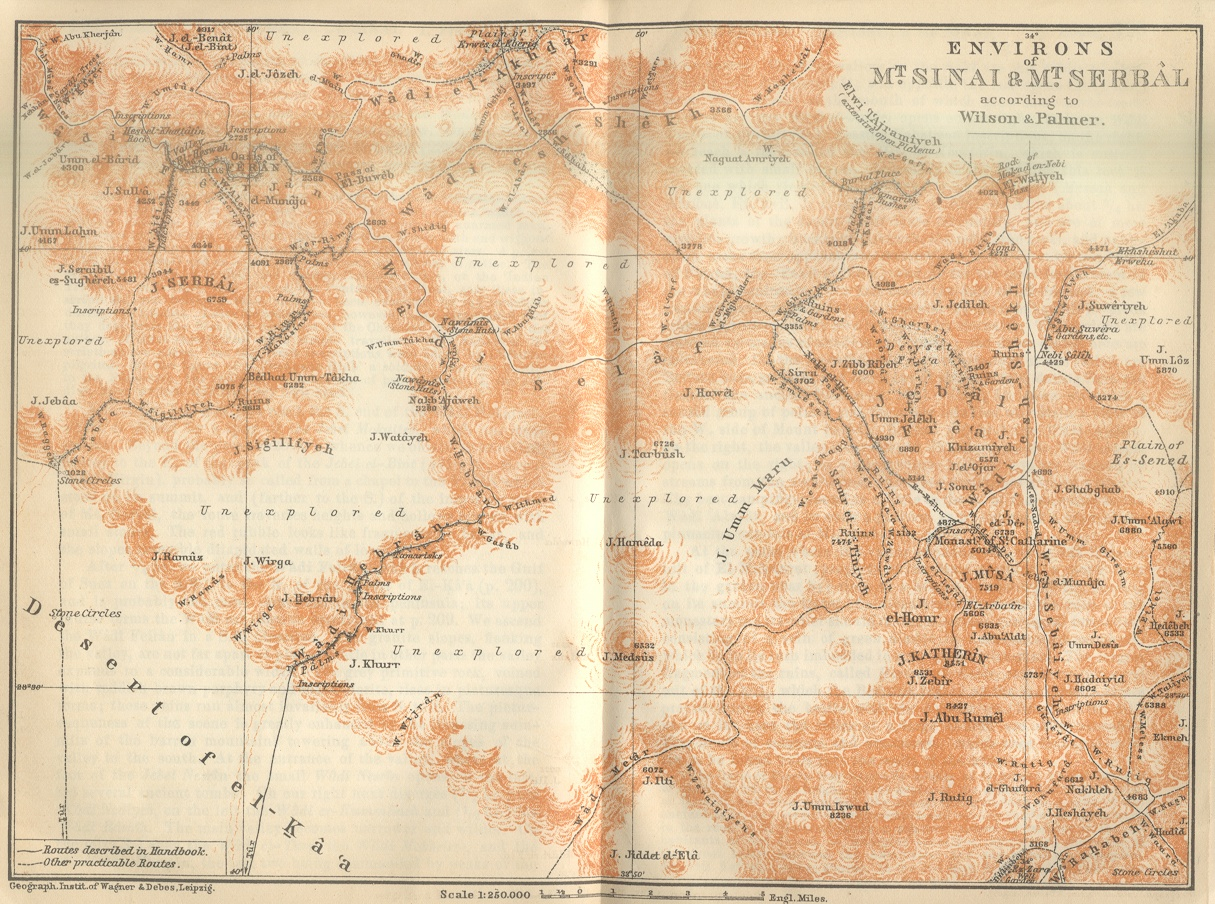
\includegraphics[clip,trim=5cm 2cm 9cm 1cm,width=\linewidth]{OldBookArt--MapImages-173.jpg}
\vfill
{\large \textit{This material is Open Game Content, and is licensed for public use under the terms of the Open Game License v1.0a.}\\
\today}
\end{center}

\pagebreak
\sffamily
\pagestyle{plain}
\raggedbottom

%%%%%%%%%%%%%%%%%%%%%%%%%%%%%%%%%%%%%%%%%%%%%%%%%%
%%%%%%%%%%%%%%%%%%%%%%%%%%%%%%%%%%%%%%%%%%%%%%%%%%
%%% Table of Contents
%%%%%%%%%%%%%%%%%%%%%%%%%%%%%%%%%%%%%%%%%%%%%%%%%%
%%%%%%%%%%%%%%%%%%%%%%%%%%%%%%%%%%%%%%%%%%%%%%%%%%
\renewcommand{\contentsname}{Table of Contents}
\setcounter{tocdepth}{1}
\tableofcontents

%%%%%%%%%%%%%%%%%%%%%%%%%%%%%%%%%%%%%%%%%%%%%%%%%%
%%%%%%%%%%%%%%%%%%%%%%%%%%%%%%%%%%%%%%%%%%%%%%%%%%
%%% Main Content %%%
%%%%%%%%%%%%%%%%%%%%%%%%%%%%%%%%%%%%%%%%%%%%%%%%%%
%%%%%%%%%%%%%%%%%%%%%%%%%%%%%%%%%%%%%%%%%%%%%%%%%%

%% Primary Chapters Here

\clearpage

\chapter{Introduction}
\section{What is a Role-playing Game?}
foo
\section{What You Need To Play}
foo
\section{The Core Mechanic}
foo
\section{Creating a Character}
foo
%%%%%%%%%%%%%%%%%%%%%%%%
%%Race Chapter Formatting
%%%%%%%%%%%%%%%%%%%%%%%%
\newcommand{\race}{placeholder}

\newcommand{\racedescription}[1]{\indent\ability{Physical Description}{#1}}
\newcommand{\racepersonality}[1]{\indent\ability{Personality}{#1}}
\newcommand{\racesociety}[1]{\indent\ability{Society}{#1}}
\newcommand{\racealignment}[1]{\indent\ability{Alignment}{#1}}

\newcommand{\type}[1]{\ability{Type}{#1}\\}
\newcommand{\size}[1]{\ability{Size}{#1}\\}
\newcommand{\speed}[1]{\ability{Speed}{#1 feet}\\}
\newcommand{\scores}[1]{\ability{Racial Ability Score Modifiers}{#1}\\}
\newcommand{\racialtraits}[1]{\ability{Unique Racial Traits}{#1}\\}
\newcommand{\racetrait}[2]{\newline\textbullet{ \ability{#1}{#2}}}
\newcommand{\senses}[1]{\ability{Senses}{#1}\\}
\newcommand{\autolanguages}[1]{\ability{Automatic Languages}{#1}\\}
\newcommand{\bonuslanguages}[1]{\ability{Bonus Languages}{#1}\\}
\newcommand{\favoredclasses}[1]{\ability{Favored Classes}{#1}\\}
\newcommand{\male}[4]{Male &#1 &#2 &#3 &#4\\}
\newcommand{\female}[4]{Female &#1 &#2 &#3 &#4\\}

\newenvironment{racetable}
{
\tabulinesep=1mm
\noindent
\begin{tabu} to \columnwidth {X}
\header\textbf{\race ~Racial Traits} \\ \hline
\end{tabu}
\vspace{-.1em}
\rowcolors{1}{colortwo}{colorone}
\begin{tabu} to \columnwidth {X [1, l]}
}{
\hline
\end{tabu}
}

\newcommand{\agetable}[4]{
\tabulinesep=1mm
\noindent
\begin{tabu} to \columnwidth {X}
\header\textbf{\race ~Starting Age} \\ \hline
\end{tabu}
\vspace{-.15em}
\rowcolors{1}{colortwo}{colorone}
\begin{tabu} to \columnwidth {X X X X}
\textbf{Adulthood:} &\textbf{Simple:} &\textbf{Moderate:} &\textbf{Complex:} \\
#1 Years &#2 &#3 &#4 \\ \hline
\end{tabu}
}

\newenvironment{heightweighttable}
{
\tabulinesep=1mm
\noindent
\begin{tabu} to \columnwidth {X}
\header\textbf{\race ~Height and Weight} \\ \hline
\end{tabu}
\vspace{-.5em}
\rowcolors{1}{colortwo}{colorone}
\begin{tabu} to \columnwidth {X X X X X}
\textbf{Gender} &\textbf{Base Height} &\textbf{Height Mod.} &\textbf{Base Weight} &\textbf{Weight Mod.} \\
}{
\hline
\end{tabu}
}

\newenvironment{raceleft}
{
\vspace{0pt}
\begin{minipage}[t]{0.5\linewidth}
}{
\end{minipage}
}

\newenvironment{raceright}
{\begin{minipage}[t]{0.5\linewidth}
\vspace{0pt}
}{
\end{minipage}
}

\newenvironment{racebox}
{
\vspace{0pt}
%\nointerlineskip
\begin{minipage}[t][0.49\textheight][t]{\textwidth}
}{
\end{minipage}
}


\chapter{Races}

\raceentry{Aasimar}{``My ancestors were more beautiful than you can imagine."}\\
\begin{multicols}{2}
Aasimar are humans that have a beautiful outsider, usually but not always a celestial, somewhere in their ancestry. \linebreak
\indent\textbf{Personality: }Though mostly human, an aasimar's immortal heritage influences their mental development. Aasimar tend toward more extreme personalities, being especially quiet and introspective or particularly loud and boisterous. Most aasimar are very opinionated, and have strongly held beleifs.\linebreak
\indent\textbf{Physical Description: }Aasimar look like especially beautiful humans, though they sometimes bear vestiges of their ancestry that denote them as being different (strangely colored eyes, silver-blonder or white hair, slightly `off' facial features).\linebreak
\indent\textbf{Society: }Aasimar are typically born and raised in human societies, and gain the same customs of that culture.\linebreak
\indent\textbf{Alignment: }Most aasimar are the descendants of celestials, and tend towards the good alignments. Rarely, an aasimar might instead have an infernal heritage, being the descendant of an erinyes or succubus. Such aasimar instead tend towards an evil alignment.\linebreak

\columnbreak

\racetable
\type{Outsider (Native and Human Subtype)}
\size{Medium}
\speed{30 foot}
\standardsenses
\scores{+2 Wisdom, +2 Charisma}
\racespecial{
\fakeitem{\spell{Light} \sla : An Aasimar with a Charisma of at least 10 may cast \spell{light} as a spell-like ability with a caster level equal to their character level once per day.} \linebreak
\fakeitem{+2 bonus to Spot, and Listen checks.}
}
\autolanguages{Common}
\bonuslanguages{Abyssal, Aquan, Auran, Celestial, Formian, Ignan, Slaad, Sylvan, Terran.}
\favoredclasses{Paladin and Sorcerer}
\end{tabu}

\vspace{\baselineskip}
\agetable{20}{+1d6}{+2d6}{+3d6}

\vspace{\baselineskip}
\male{4' 7"}{+2d8}{90 lb.}{x(2d4)}
\female{4' 5"}{+2d8}{80 lb.}{x(2d4)}
\heightweighttable
\end{multicols}

\begin{racebox}
\raceentry{Drow}{``Time to die for the Spider Queen."}
\begin{multicols}{2}

\begin{racetable}
\type{Humanoid (Elf Subtype)}
\size{Medium}
\scores{+2 Dexterity, -2 Constitution}
\speed{30}
\senses{Darkvision 120'}
\autolanguages{Elvish}
\bonuslanguages{Abyssal, Beholder, Common, Draconic, Drow Sign Language, Dwarvish, Gnome, Kuo-Toa, Terran, Undercommon}
\favoredclasses{Cleric and Wizard}
\end{racetable}

\vspace{\baselineskip}
\agetable{20}{+1d6}{+2d6}{+3d6}

\vspace{\baselineskip}
\begin{heightweighttable}
\male{4' 7"}{+2d8}{90 lb.}{x(2d4)}
\female{4' 5"}{+2d8}{80 lb.}{x(2d4)}
\end{heightweighttable}

\racialtraits{
\racetrait{Daylight Sensitivity}{While in brightly lit surroundings (such as a daylight spell), a Drow suffers a -2 penalty to attack rolls and precision-based skill checks.}
\racetrait{Innate Magic}{Drow with a Charisma of at least 10 may cast deeper darkness (duration 4 hours), and fairie fire as spell-like abilities with a caster level equal to their character level once per day each.}
\racetrait{Magic Resistant}{+2 bonus to saving throws against spells and spell-like abilities.}
\racetrait{Skill Bonus}{+2 bonus to Spot and Listen checks.}
\racetrait{Elven Trance}{Drow never sleep and are immune to sleep effects. Drow must still perform their 4 hour daily trance to stay coherent and rested.}
\racetrait{Interesting Times}{Drow live an exceedingly interesting life and every Drow has proficiency with the rapier and an exotic ranged weapon of their choice.}
}

\end{multicols}
\end{racebox}

\raceentry{Dwarf}
\quot{``I remember that...''}

\listone
		\item Medium Size
		\item 20' movement
		\item Humanoid Type (Dwarf Subtype)
		\item +2 Constitution, -2 Charisma
		\item Dwarves can move up to their full speed even when wearing medium or heavy armor or when carrying a medium or heavy load
		\item Darkvision: Dwarves can see up to 60 feet in the dark.
		\item Stonecunning: This ability grants a dwarf a +2 racial bonus on Search checks to notice unusual stonework, such as sliding walls, stonework traps, new construction (even when built to match the old), unsafe stone surfaces, shaky stone ceilings, and the like. Something that isn’t stone but that is disguised as stone also counts as unusual stonework. A dwarf who merely comes within 10 feet of unusual stonework can make a Search check as if he were actively searching, and a dwarf can use the Search skill to find stonework traps as a rogue can. A dwarf can also intuit depth, sensing his approximate depth underground as naturally as a human can sense which way is up.
		\item Weapon Familiarity: Dwarves may treat dwarven waraxes and dwarven urgroshes as martial weapons, rather than exotic weapons.
		\item Stability: A dwarf gains a +4 bonus on ability checks made to resist being bull rushed or tripped when standing on the ground (but not when climbing, flying, riding, or otherwise not standing firmly on the ground).
		\item +2 racial bonus on saving throws against poison.
		\item +2 racial bonus on saving throws against spells and spell-like effects.
		\item +1 racial bonus on attack rolls against orcs and goblinoids.
		\item +4 dodge bonus to Armor Class against monsters of the giant type. Any time a creature loses its Dexterity bonus (if any) to Armor Class, such as when it’s caught flat-footed, it loses its dodge bonus, too.
		\item +2 racial bonus on Appraise checks that are related to stone or metal items.
		\item +2 racial bonus on Craft checks that are related to stone or metal.
		\item Favored class: Fighter
		\item Automatic Languages: Common and Dwarven.
		\item Bonus Languages: Giant, Gnome, Goblin, Orc, Terran, and Undercommon.
\end{list}


\raceentry{Elf}
\quot{``You shall never harm my beautiful trees!''}

\listone
		\item Medium Size
		\item Humanoid Type (Elf Subtype)
		\item 30' movement
		\item +2 Dexterity, -2 Constitution
		\item Low Light Vision: Elves can see twice as far as a human in poor lighting.
		\item Weapon Proficiency: Elves are proficient with the longsword, rapier, longbow (including composite longbow), and shortbow (including composite shortbow).
		\item +2 racial bonus on Listen, Search, and Spot checks. An elf who merely passes within 5 feet of a secret or concealed door is entitled to a Search check to notice it as if she were actively looking for it.
		\item Favored Class: Wizard.
		\item Automatic Languages: Common and Elven. 
		\item Bonus Languages: Draconic, Gnoll, Gnome, Goblin, Orc, and Sylvan.
\end{list}

\raceentry{Feytouched}
\quot{``All my life, I have never fit in. Not in town, not in the forest. In some integral fashion I am unlike those around me, and I believe it is my fate to live and die alone."}

\listone
		\item Medium Size
    \item Fey Type
    \item 30' movement
    \item Low-Light Vision: Feytouched can twice as far as a human in poor lighting.
    \item +2 Dexterity, +2 Charisma, -2 Constitution. Feytouched are graceful and those which are not beautiful are terrifying, but they are fragile like flowers.
    \item Immunity to [Compulsion] Effects
    \item Magic Affinity: Every Feytouched is different, and marked by the signature magics of the fey in a different manner. Every Feytouched has one spell that can be used once per day as a spell-like ability. This spell is chosen at 1st level and cannot be changed. Any 1st level Illusion or Enchantment spell from the Sorcerer/Wizard list is fair game, and the save DC is Charisma-based.
    \item Favored Class: Bard
    \item Feytouched speak Common and Sylvan. Bonus Languages may be selected from the following list:
      Aquan, Auran, Elvish, Draconic, Dwarvish, Druidic, Goblin, Gnoll, Gnome, Halfling.
\end{list}

\begin{racebox}
\raceentry{Gnome}{``What's that you say little mole? Kobolds in the well!?"}
\begin{multicols}{2}

\begin{racetable}
\type{Humanoid (Gnome subtype)}
\size{Small}
\scores{+2 Constitution, --2 Strength}
\speed{20}
\senses{Low Light Vision}
\autolanguages{Common and Gnome}
\bonuslanguages{Draconic, Dwarven, Elven, Giant, Goblin, and Orc. In addition, a gnome can speak with a burrowing mammal (a badger, fox, rabbit, or the like).}
\favoredclasses{Bard}
\end{racetable}

Nothing until we find or write it.

\racedescription{NYW}

\racepersonality{NYW}

\racesociety{NYW}

\racealignment{NYW}

\racialtraits{
\racetrait{Weapon Familiarity}{Gnomes may treat gnome hooked hammers as martial weapons rather than exotic weapons.}
\racetrait{+2 racial bonus on saving throws against illusions.}
\racetrait{Add +1 to the Difficulty Class for all saving throws against illusion spells cast by gnomes. This adjustment stacks with those from similar effects.}
\racetrait{+1 racial bonus on attack rolls against kobolds and goblinoids.}
\racetrait{+4 dodge bonus to Armor Class against monsters of the giant type.}
\racetrait{+2 racial bonus on Listen checks.}
\racetrait{+2 racial bonus on Craft (alchemy) checks.}
\racetrait{Spell-Like Abilities: 1/day—speak with animals (burrowing mammal only, duration 1 minute). A gnome with a Charisma score of at least 10 also has the following spell-like abilities: 1/day—dancing lights, ghost sound, prestidigitation. Caster level 1st; save DC 10 + gnome’s Cha modifier + spell level.} % I'm pretty sure there's a much better way to format this, say by using the \sla used for aasimar. That Cha req goofs it up.
}


%\columnbreak

\vspace{\baselineskip}
\agetable{40}{+4d6}{+6d6}{+9d6}

\vspace{\baselineskip}
\begin{heightweighttable}
\male{3' 0"}{+2d4}{40 lb.}{x(1)}
\female{2' 10"}{+2d4}{35 lb.}{x(1)}
\end{heightweighttable}
\end{multicols}
\end{racebox}

\raceentry{Goblin}
\quot{``You weren't hired to think. You were hired because you have opposable thumbs."}

\listone
    \item Small Size
    \item 30' movement (despite small size).
    \item Humanoid Type (Goblinoid subtype)
    \item Darkvision: Goblins can see up to 60 feet in the dark.
    \item +2 Dexterity, -2 Strength, -2 Charisma
    \item +4 bonus to Move Silently and Ride checks.
    \item Bonus Feat: Mounted Combat
    \item Goblins benefit from an ancient pact with the Worgs, and every Goblin receives a +2 bonus to any Bluff, Diplomacy, Handle Animal, Sense Motive, or Survival check made with respect to a Worg.
    \item Favored Classes: Rogue and Wizard
    \item Automatic Languages: Common, Goblin
    \item Bonus Languages: Draconic, Elvish, Dwarvish, Giant, Gnoll, Infernal, Orcish, Undercommon, and Worg.
\end{list}
\raceentry{Half-Elf}
\quot{``I don't fit in anywhere, please, listen to me cry.''}

\listone
		\item Medium Size
		\item 30' Movement
		\item Humanoid Type
		\item Low-Light Vision: Half-Elves can see twice as humans in poor lighting.
		\item Immunity to sleep spells and similar magical effects, and a +2 racial bonus on saving throws against enchantment spells or effects.
		\item +1 racial bonus on Listen, Search, and Spot checks.
		\item +2 racial bonus on Diplomacy and Gather Information checks.
		\item Elven Blood: For all effects related to race, a half-elf is considered an elf.
		\item Favored Class: Any
		\item Automatic Languages: Common and Elven.
		\item Bonus Languages: Any (other than secret languages, such as Druidic).
\end{list}
\subsection{Halfling}
\quot{``Where are we going Mr. Frodo?''}

\listone
		\item Small Size
		\item 20' movement
		\item +2 Dexterity, -2 Strength
		\item +2 racial bonus on Climb, Jump, Listen, and Move Silently checks.
		\item +1 racial bonus on all saving throws.
		\item +2 morale bonus on saving throws against fear: This bonus stacks with the halfling’s +1 bonus on saving throws in general.
		\item +1 racial bonus on attack rolls with thrown weapons and slings.
		\item Favored Class: Rogue
		\item Automatic Languages: Common and Halfling.
		\item Bonus Languages: Dwarven, Elven, Gnome, Goblin, and Orc.
\end{list}		

\raceentry{Half-Orc}
\quot{``I don't fit in anywhere, but you may be surprised to know that this dagger fits all kinds of places."}

\listone
    \item Medium Size
    \item 30' movement
    \item Humanoid Type (Orc and Human subtype)
    \item Darkvision: Half-Orcs can see up to 60 feet in the dark.
    \item +2 Strength
    \item +2 to Intimidate, Gather Information, and Survival checks.
    \item Favored Classes: Assassin and Barbarian
    \item Automatic Languages: Orc, Common
    \item Bonus Languages: Any.
\end{list}
\raceentry{Hobgoblin}
\quot{``That's some tough talk from a man who wears a basket on his head."}

\listone
    \item Medium Size
    \item 30' movement.
    \item Humanoid Type (Goblinoid subtype)
    \item Darkvision: Hobgoblins can see up to 60 feet in the dark.
    \item +2 Dexterity, +2 Constitution
    \item +4 bonus to Move Silently checks.
    \item Favored Classes: Fighter and Samurai
    \item Automatic Languages: Common, Goblin
    \item Bonus Languages: Draconic, Elvish, Dwarvish, Giant, Gnoll, Ignan, Infernal, Orcish.
\end{list}
\raceentry{Human}
\quot{``Yeah, I'm pretty normal.''}

\listone
	\item Medium Size
	\item 30' movement.
	\item Humanoid Type (Human subtype)
	\item 1 extra feat at 1st level.
	\item 4 extra skill points at 1st level and 1 extra skill point at each additional level.
	\item Favored Class: Any. When determining whether a multiclass human takes an experience point penalty, his or her highest-level class does not count.
	\item Automatic Language: Common. 
	\item Bonus Languages: Any (other than secret languages, such as Druidic). See the Speak Language skill.
\end{list}
\raceentry{Kobold}
\quot{``Aieeeeeeeee!''}

\listone
		\item Small Size
		\item 30' movement (despite small size)
		\item Humanoid Type (Reptilian subtype)
		\item Darkvision: Kobolds can see up to 60 feet in the dark.
		\item -4 Strength, +2 Dexterity, -2 Constitution
		\item Racial Skills: A kobold character has a +2 racial bonus on Craft (trapmaking), Profession (miner), and Search checks.
		\item +1 natural armor bonus.
		\item Light sensitivity: Kobolds are dazzled in bright sunlight or within the radius of a daylight spell. 
		\item Favored Class: Sorcerer.
		\item Automatic Languages: Draconic.
		\item Bonus Languages: Common, Undercommon.
\end{list}
\raceentry{Orc}
\quot{``Waaarrrggghhhh!"}

\listone
    \item Medium Size
    \item 30' movement.
    \item Humanoid Type (Orc subtype)
    \item Darkvision: Orcs can see up to 60 feet in the dark.
    \item +4 Strength, -2 Intelligence, -2 Charisma, -2 Wisdom
    \item Daylight Sensitivity: While in brightly lit surroundings (such as a daylight spell), an Orc suffers the dazzled condition and is thus at a -1 penalty to attack rolls and precision-based skill checks.
    \item +2 bonus to saving throws vs. Poison and Disease.
    \item Immunity to ingested poisons.
    \item +2 to Jump and Survival checks.
    \item Favored Classes: Barbarian and Cleric
    \item Automatic Languages: Orc, Common
    \item Bonus Languages: Dwarvish, Elvish, Giant, Gnoll, Goblin, Sylvan, Undercommon.
\end{list}
\raceentry{Tiefling}
\quot{``My ancestors were more evil than you will ever know, but let's see how I compare.''}

\listone
    \item Medium Size
    \item 30' movement.
    \item Outsider Type (Native and Human subtype)
    \item Darkvision: Tieflings can see up to 60 feet in the dark.
    \item +2 Dexterity, +2 Intelligence, -2 Charisma
    \item Tieflings with a Charisma of at least 10 may cast darkness as a spell-like ability with a caster level equal to their character level once per day.
    \item +2 bonus to Bluff, Hide, and Move Silently checks.
    \item Favored Classes: Rogue and True Fiend
    \item Automatic Languages: Common
    \item Bonus Languages: Abyssal, Aquan, Auran, Celestial, Formian, Ignan, Slaad, Sylvan, Terran.
\end{list}
%%%%%%%%%%%%%%%%%%%%%%%%
%%Class Chapter Formatting
%%%%%%%%%%%%%%%%%%%%%%%%

\newcommand{\class}{placeholder}
%Holds the class's name, as defined by \classentry

\newenvironment{classpreamble}{
%\centering
%\rowcolors{1}{colorone}{colortwo}
%\begin{tabu} to \textwidth {X}
}{
%\end{tabu}
}

\newcommand{\desc}[1]{\noindent#1 \\}
\newcommand{\playingaclass}[1]{\indent\ability{Playing a \class : }{#1}\\}
\newcommand{\hitdie}[1]{\indent\ability{Hit Die: }{#1}\\}
\newcommand{\alignment}[1]{\indent\ability{Alignment: }{#1}\\}
\newcommand{\races}[1]{\indent\ability{Races: }{#1}\\}
\newcommand{\startinggold}[1]{\indent\ability{Starting Gold: }{#1}\\}
\newcommand{\startingage}[1]{\indent\ability{Starting Age: }{#1}\\}  
\newcommand{\skillpoints}[1]{\indent\ability{Skill Points per Level: }{#1 + Intelligence Bonus}\\}
\newcommand{\classskills}[1]{\newline\indent\ability{Class Skills: }{The {\class}'s class skills (and the key ability for each skill) are #1}\\}

%\newcommand{\desc}[1]{ #1 \\}
%\newcommand{\playingaclass}[1]{\selectfont\ability{Playing a \class : }{#1}\\}
%\newcommand{\hitdie}[1]{\ability{Hit Die: }{#1}\\}
%\newcommand{\alignment}[1]{\ability{Alignment: }{#1}\\}
%\newcommand{\races}[1]{\ability{Races: }{#1}\\}
%\newcommand{\startinggold}[1]{\ability{Starting Gold: }{#1}\\}
%\newcommand{\startingage}[1]{\ability{Starting Age: }{#1}\\}  
%\newcommand{\skillpoints}[1]{\ability{Skill Points per Level: }{#1 + Intelligence Bonus}\\}
%\newcommand{\classskills}[1]{\ability{Class Skills: }{The {\class}'s class skills (and the key ability for each skill) are #1}\\}


\newcommand{\startclassfeatures}{
 \smallskip\noindent All of the following are class features of the \class ~class.}
%place before actual class features entries.

\newcommand{\proficiencies}[1]{
 \ability{Weapon and Armor Proficiencies:}{The \class ~is proficient with #1}}
%Displays proficiencies with minimal input, implimentation looks like \proficiencies{the proficiencies}

\newcommand{\classfeature}[2]{
  \ability{#1}{#2}}
%No functional difference from \ability currently

%%%%Class Table Commands

\newcommand{\gbab}{\empty}
\newcommand{\mbab}{\empty}
\newcommand{\fort}{\empty}
\newcommand{\refl}{\empty}
\newcommand{\will}{\empty}
%Creates new commands for use in \ifx statements for formatting purposes.

\newcommand{\goodbab}{\renewcommand{\gbab}{\empty}\renewcommand{\mbab}{a}}
\newcommand{\modebab}{\renewcommand{\gbab}{a}\renewcommand{\mbab}{\empty}}
\newcommand{\poorbab}{\renewcommand{\gbab}{a}\renewcommand{\mbab}{a}}
%A set of commands to tell LaTeX what BAB progression the class has. Only one should be called per class.

\newcommand{\goodfor}{\renewcommand{\fort}{\empty}}
\newcommand{\poorfor}{\renewcommand{\fort}{a}}
%A set of commands to tell LaTeX what Fortitude progression the class has. Only one should be called per class.

\newcommand{\goodref}{\renewcommand{\refl}{\empty}}
\newcommand{\poorref}{\renewcommand{\refl}{a}}
%A set of commands to tell LaTeX what Reflex progression the class has. Only one should be called per class.

\newcommand{\goodwil}{\renewcommand{\will}{\empty}}
\newcommand{\poorwil}{\renewcommand{\will}{a}}
%A set of commands to tell LaTeX what Will progression the class has. Only one should be called per class.

\newenvironment{classtable}[1]
{
\centering
\rowcolors{1}{colorone}{colortwo}
\begin{tabu} to \textwidth {p{.275in} l p{0.275in} p{0.275in} p{0.275in} X l l l l} 
\rowcolor{headercolor} Level & Base Attack & Fort. & Ref. & Will & Special #1 \\
}{
\hline
\end{tabu}
}
%A a new environment that sets up the class tables. Include the \level commands between \begin{classtable}.

\newenvironment{minorcastingclasstable}
{
%\table[htb]
%\center
\centering
\rowcolors{1}{colorone}{colortwo}
\begin{tabu}to \textwidth{p{.275in}lp{0.275in}p{0.275in}p{0.275in}Xccccccc}
\rowcolor{headercolor} & & & & & &\multicolumn{7}{c}{Spells Per Day (By Level)} \\
\rowcolor{headercolor} Level & Base Attack & Fort. & Ref. & Will & Special &0&1&2&3&4&5&6\\
}{
\hline
\end{tabu}
%\endcenter
%\endtable
}
%A a new environment similar to classtable, but with columns for a minor (zero through six) spell slot progression.

\newenvironment{fullcastingclasstable}
{
\table[htb]
\center
\rowcolors{1}{colorone}{colortwo}
\begin{tabu}to \textwidth{p{.275in}lp{0.275in}p{0.275in}p{0.275in}Xcccccccccc}
\rowcolor{headercolor} & & & & & &\multicolumn{10}{c}{Spells Per Day (By Level)} \\
\rowcolor{headercolor} Level & Base Attack & Fort. & Ref. & Will & Special &0&1&2&3&4&5&6&7&8&9\\
}{
\hline
\end{tabu}
\endcenter
\endtable
}
%Another environment for class tables, this one for full (0 through 9) spell slot progression.

\newcommand{\levelone}[1]{
\hline
1st  & \ifx\gbab\isempty +1 \else\ifx\mbab\isempty +0 \else +0 \fi \fi
	 & \ifx\fort\isempty +2 \else +0 \fi
	 & \ifx\refl\isempty +2 \else +0 \fi
	 & \ifx\will\isempty +2 \else +0 \fi
	 & #1 \\}
%A command that declares a table row within the class feature table.

\newcommand{\leveltwo}[1]{
2nd  & \ifx\gbab\isempty +2 \else\ifx\mbab\isempty +1 \else +1 \fi \fi
	 & \ifx\fort\isempty +3 \else +0 \fi
	 & \ifx\refl\isempty +3 \else +0 \fi
	 & \ifx\will\isempty +3 \else +0 \fi
	 & #1 \\}
%A command that declares a table row within the class feature table.

\newcommand{\levelthree}[1]{
3rd  & \ifx\gbab\isempty +3 \else\ifx\mbab\isempty +2 \else +1 \fi \fi
	 & \ifx\fort\isempty +3 \else +1 \fi
	 & \ifx\refl\isempty +3 \else +1 \fi
	 & \ifx\will\isempty +3 \else +1 \fi
	 & #1 \\}
%A command that declares a table row within the class feature table.

\newcommand{\levelfour}[1]{
4th  & \ifx\gbab\isempty +4 \else\ifx\mbab\isempty +3 \else +2 \fi \fi
	 & \ifx\fort\isempty +4 \else +1 \fi
	 & \ifx\refl\isempty +4 \else +1 \fi
	 & \ifx\will\isempty +4 \else +1 \fi
	 & #1 \\}
%A command that declares a table row within the class feature table.

\newcommand{\levelfive}[1]{
5th  & \ifx\gbab\isempty +5 \else\ifx\mbab\isempty +3 \else +2 \fi \fi
	 & \ifx\fort\isempty +4 \else +1 \fi
	 & \ifx\refl\isempty +4 \else +1 \fi
	 & \ifx\will\isempty +4 \else +1 \fi
	 & #1 \\}
%A command that declares a table row within the class feature table.
	 
\newcommand{\levelsix}[1]{
6th  & \ifx\gbab\isempty +6/+1 \else\ifx\mbab\isempty +4 \else +3 \fi \fi
	 & \ifx\fort\isempty +5 \else +2 \fi
	 & \ifx\refl\isempty +5 \else +2 \fi
	 & \ifx\will\isempty +5 \else +2 \fi
	 & #1 \\}
%A command that declares a table row within the class feature table.

\newcommand{\levelseven}[1]{
7th  & \ifx\gbab\isempty +7/+2 \else\ifx\mbab\isempty +5 \else +3 \fi \fi
	 & \ifx\fort\isempty +5 \else +2 \fi
	 & \ifx\refl\isempty +5 \else +2 \fi
	 & \ifx\will\isempty +5 \else +2 \fi
	 & #1 \\}
%A command that declares a table row within the class feature table.
	 
\newcommand{\leveleight}[1]{
8th  & \ifx\gbab\isempty +8/+3 \else\ifx\mbab\isempty +6/+1 \else +4 \fi \fi
	 & \ifx\fort\isempty +6 \else +2 \fi
	 & \ifx\refl\isempty +6 \else +2 \fi
	 & \ifx\will\isempty +6 \else +2 \fi
	 & #1 \\}
%A command that declares a table row within the class feature table.
	 
\newcommand{\levelnine}[1]{
9th  & \ifx\gbab\isempty +9/+4 \else\ifx\mbab\isempty +6/+1 \else +4 \fi \fi
	 & \ifx\fort\isempty +6 \else +3 \fi
	 & \ifx\refl\isempty +6 \else +3 \fi
	 & \ifx\will\isempty +6 \else +3 \fi
	 & #1 \\}
%A command that declares a table row within the class feature table.
	 
\newcommand{\levelten}[1]{
10th & \ifx\gbab\isempty +10/+5 \else\ifx\mbab\isempty +7/+2 \else +5 \fi \fi
	 & \ifx\fort\isempty +7 \else +3 \fi
	 & \ifx\refl\isempty +7 \else +3 \fi
	 & \ifx\will\isempty +7 \else +3 \fi
	 & #1 \\}
%A command that declares a table row within the class feature table.
	 
\newcommand{\leveleleven}[1]{
11th & \ifx\gbab\isempty +11/+6/+6 \else\ifx\mbab\isempty +8/+3 \else +5 \fi \fi
	 & \ifx\fort\isempty +7 \else +3 \fi
	 & \ifx\refl\isempty +7 \else +3 \fi
	 & \ifx\will\isempty +7 \else +3 \fi
	 & #1 \\}
%A command that declares a table row within the class feature table.
	 
\newcommand{\leveltwelve}[1]{
12th & \ifx\gbab\isempty +12/+7/+7 \else\ifx\mbab\isempty +9/+4 \else +6/+1 \fi \fi
	 & \ifx\fort\isempty +8 \else +4 \fi
	 & \ifx\refl\isempty +8 \else +4 \fi
	 & \ifx\will\isempty +8 \else +4 \fi
	 & #1 \\}
%A command that declares a table row within the class feature table.
	 
\newcommand{\levelthirteen}[1]{
13th & \ifx\gbab\isempty +13/+8/+8 \else\ifx\mbab\isempty +9/+4 \else +6/+1 \fi \fi
	 & \ifx\fort\isempty +8 \else +4 \fi
	 & \ifx\refl\isempty +8 \else +4 \fi
	 & \ifx\will\isempty +8 \else +4 \fi
	 & #1 \\}
%A command that declares a table row within the class feature table.
	 
\newcommand{\levelfourteen}[1]{
14th & \ifx\gbab\isempty +14/+9/+9 \else\ifx\mbab\isempty +10/+5 \else +7/+2 \fi \fi
	 & \ifx\fort\isempty +9 \else +4 \fi
	 & \ifx\refl\isempty +9 \else +4 \fi
	 & \ifx\will\isempty +9 \else +4 \fi
	 & #1 \\}
%A command that declares a table row within the class feature table.
	 
\newcommand{\levelfifteen}[1]{
15th & \ifx\gbab\isempty +15/+10/+10 \else\ifx\mbab\isempty +11/+6/+6 \else +7/+2 \fi \fi
	 & \ifx\fort\isempty +9 \else +5 \fi
	 & \ifx\refl\isempty +9 \else +5 \fi
	 & \ifx\will\isempty +9 \else +5 \fi
	 & #1 \\}
%A command that declares a table row within the class feature table.
	 
\newcommand{\levelsixteen}[1]{
16th & \ifx\gbab\isempty +16/+11/+11/+11 \else\ifx\mbab\isempty +12/+7/+7 \else +8/+3 \fi \fi
	 & \ifx\fort\isempty +10 \else +5 \fi
	 & \ifx\refl\isempty +10 \else +5 \fi
	 & \ifx\will\isempty +10 \else +5 \fi
	 & #1 \\}
%A command that declares a table row within the class feature table.
	 
\newcommand{\levelseventeen}[1]{
17th & \ifx\gbab\isempty +17/+12/+12/+12 \else\ifx\mbab\isempty +12/+7/+7 \else +8/+3 \fi \fi
	 & \ifx\fort\isempty +10 \else +5 \fi
	 & \ifx\refl\isempty +10 \else +5 \fi
	 & \ifx\will\isempty +10 \else +5 \fi
	 & #1 \\}
%A command that declares a table row within the class feature table.
	 
\newcommand{\leveleighteen}[1]{
18th & \ifx\gbab\isempty +18/+13/+13/+13 \else\ifx\mbab\isempty +13/+8/+8 \else +9/+4 \fi \fi
	 & \ifx\fort\isempty +11 \else +6 \fi
	 & \ifx\refl\isempty +11 \else +6 \fi
	 & \ifx\will\isempty +11 \else +6 \fi
	 & #1 \\}
%A command that declares a table row within the class feature table.
	 
\newcommand{\levelnineteen}[1]{
19th & \ifx\gbab\isempty +19/+14/+14/+14 \else\ifx\mbab\isempty +14/+9/+9 \else +9/+4 \fi \fi
	 & \ifx\fort\isempty +11 \else +6 \fi
	 & \ifx\refl\isempty +11 \else +6 \fi
	 & \ifx\will\isempty +11 \else +6 \fi
	 & #1 \\}
%A command that declares a table row within the class feature table.
	 
\newcommand{\leveltwenty}[1]{
20th & \ifx\gbab\isempty +20/+15/+15/+15 \else\ifx\mbab\isempty +15/+10/+10 \else +10/+5 \fi \fi
	 & \ifx\fort\isempty +12 \else +6 \fi
	 & \ifx\refl\isempty +12 \else +6 \fi
	 & \ifx\will\isempty +12 \else +6 \fi
	 & #1 \\}
%A command that declares a table row within the class feature table.

\newmdenv[hidealllines=true,backgroundcolor=gray!20]{optionbox}

\newcommand{\option}[1]{
  \renewmdenv[hidealllines=true,backgroundcolor=colorone]{optionbox}
   \begin{optionbox}\noindent{#1}\end{optionbox}
   ~\\*
}

\newenvironment{optional}{
\colorlet{colortwo}{white}
\colorlet{colorone}{gray!15}
}

%%%%%%%%%%%%%%%%%%%%%%%%

\chapter{Classes}
\section{Class Basics}
foo
\section{Core Classes}

\classname{Assassin} \label{class:assassin}
\vspace{-8pt}
\quot{"I kill people. Individually, you are a person. Collectively, I think you count as people."}

\desc{An assassin is a master of the art of killing, a vicious weapon honed by experience and inclination to learn the myriad ways to end a life. Unlike common warriors or rogues, an Assassin does not study various fighting arts or muddle his training with martial dirty tricks, he instead studies the anatomy of the various creatures of wildly different anatomies and forms of existence, and he uses this knowledge to place his blows in areas vital for biological or mystical reasons. Stealth and sudden violence are his hallmarks, and various exotic tools and killing methods become his tools.}

\desc{While most societies consider assassination to be a vile art, or at best a dishonorable or unvalorous one, the reasons that drive these killers vary. Cold-hearted mercenaries share a skill set with dedicated demon-hunters, differing only in the application of their skills. Only the most na\"ive student of ethics believes that all killing is evil, or that nobility cannot be found in a mercifully quick death.}

\ability{Alignment:}{An Assassin may be of any alignment.}

\ability{Races:}{Any}

\ability{Starting Gold:}{6d4x10 gp (150 gold)}

\ability{Starting Age:}{As Rogue.}

\ability{Hit Die:}{d6}

\ability{Class Skills:}{The Assassin's skills (and the key ability for each skill) are Balance (Dex), Bluff (Cha), Climb (Str), Concentration (Con), Craft (Int), Diplomacy (Cha), Disable Device (Int), Disguise (Cha), Gather Information (Cha), Hide (Dex), Intimidate (Cha), Jump (Str), Knowledge (all) (Int), Listen (Wis), Move Silently (Dex), Perform (Cha), Profession (Wis), Search (Int), Sense Motive (Wis), Sleight of Hand (Dex), Spellcraft (Int), Spot (Wis), Swim (Str), Tumble (Dex), and Use Magic Device (Cha).}

\ability{Skills/Level:}{6 + Intelligence Bonus}

\begin{table}[htb]
\begin{small}
\begin{tabular}{lp{1.9cm}p{0.7cm}p{0.7cm}p{0.7cm}l}
Level  &Base Attack Bonus &Fort Save &Ref Save &Will Save &Special\\
1st &+0 &+2 &+2 &+0 &Poison Use, Death Attack +3d6, Personal Immunity, Spellcasting\\
2nd &+1 &+3 &+3 &+0 &Uncanny Dodge, Death Attack +4d6\\
3rd &+2 &+3 &+3 &+1 &Hide in Plain Sight, Death Attack +5d6\\
4th &+3 &+4 &+4 &+1 &Cloak of Discretion, Death Attack +6d6\\
5th &+3 &+4 &+4 &+1 &Traps, Trapmaking, Death Attack +7d6\\
6th &+4 &+5 &+5 &+2 &Palm Weapon, Death Attack +8d6\\
7th &+5 &+5 &+5 &+2 &Full Death Attack, Death Attack +9d6\\
8th &+6/+1 &+6 &+6 &+2 &Nerve of the Assassin, Death Attack +10d6\\
9th &+6/+1 &+6 &+6 &+3 &Improved Uncanny Dodge, Death Attack +11d6\\
10th &+7/+2 &+7 &+7 &+3 &Skill Mastery, Death Attack +12d6\\
11th &+8/+3 &+7 &+7 &+3 &Poisonmaster, Death Attack +13d6\\
12th &+8/+3 &+8 &+8 &+4 &Personal Immunity, Death Attack +14d6\\
13th &+9/+4 &+8 &+8 &+4 &Exotic Method, Death Attack +15d6\\
14th &+10/+5 &+9 &+9 &+4 &Personal Immunity, Death Attack +16d6\\
15th &+11/+6/+6 &+9 &+9 &+5 &Killer's Proof, Death Attack +17d6\\
16th &+12/+7/+7 &+10 &+10 &+5 &Exotic Method, Death Attack +18d6\\
17th &+12/+7/+7 &+10 &+10 &+5 &Death by a Thousand Cuts, Death Attack +19d6\\
18th &+13/+8/+8 &+11 &+11 &+6 &Mind Blank, Death Attack +20d6\\
19th &+14/+9/+9 &+11 &+11 &+6 &Exotic Method, Death Attack +21d6\\
20th &+15/+10/+10 &+12 &+12 &+6 &Killing Strike, Death Attack +22d6\\
\end{tabular}
\end{small}
\end{table}

\begin{floatingfigure}{3.9in}
\begin{small}
\noindent\begin{tabular}{lllllllllllllllll}
 & \multicolumn{7}{c}{Assassin Spells Per Day}  &   &\multicolumn{7}{c}{Assassin Spells Known}\\
  &0 &1 &2 &3 &4 &5 &6 &  &  &0 &1 &2 &3 &4 &5 &6\\
1 &2 &- &- &- &- &- &- &  &1 &4 &- &- &- &- &- &-\\
2 &3 &0 &- &- &- &- &- &  &2 &5 &2 &- &- &- &- &-\\
3 &3 &1 &- &- &- &- &- &  &3 &6 &3 &- &- &- &- &-\\
4 &3 &2 &0 &- &- &- &- &  &4 &6 &3 &2 &- &- &- &-\\
5 &3 &3 &1 &- &- &- &- &  &5 &6 &4 &3 &- &- &- &-\\
6 &3 &3 &2 &- &- &- &- &  &6 &6 &4 &3 &- &- &- &-\\
7 &3 &3 &2 &0 &- &- &- &  &7 &6 &4 &4 &2 &- &- &-\\
8 &3 &3 &3 &1 &- &- &- &  &8 &6 &4 &4 &3 &- &- &-\\
9 &3 &3 &3 &2 &- &- &- &  &9 &6 &4 &4 &3 &- &- &-\\
10 &3 &3 &3 &2 &0 &- &- &  &10 &6 &4 &4 &4 &2 &- &-\\
11 &3 &3 &3 &3 &1 &- &- &  &11 &6 &4 &4 &4 &3 &- &-\\
12 &3 &3 &3 &3 &2 &- &- &  &12 &6 &4 &4 &4 &3 &- &-\\
13 &3 &3 &3 &3 &2 &0 &- &  &13 &6 &4 &4 &4 &4 &2 &-\\
14 &3 &3 &3 &3 &3 &1 &- &  &14 &6 &4 &4 &4 &4 &3 &-\\
15 &3 &3 &3 &3 &3 &2 &- &  &15 &6 &4 &4 &4 &4 &3 &-\\
16 &3 &3 &3 &3 &3 &2 &0 &  &16 &6 &5 &4 &4 &4 &4 &2\\
17 &3 &3 &3 &3 &3 &3 &1 &  &17 &6 &5 &5 &4 &4 &4 &3\\
18 &3 &3 &3 &3 &3 &3 &2 &  &18 &6 &5 &5 &5 &4 &4 &3\\
19 &3 &3 &3 &3 &3 &3 &3 &  &19 &6 &5 &5 &5 &5 &4 &4\\
20 &3 &3 &3 &3 &3 &3 &3 &  &20 &6 &5 &5 &5 &5 &5 &4\\
\end{tabular}
\end{small}
\end{floatingfigure}

\smallskip\noindent All of the following are Class Features of the Assassin class.

\ability{Weapon and Armor Proficiency:}{Assassins are proficient with all Light Weapons, as well as simple weapons, repeating crossbows, and hand crossbows. At first level, an Assassin gains proficiency with one Exotic Weapon of her choice. Assassins are proficient with Light Armor but not with shields.}

\ability{Spellcasting:}{The Assassin is an Arcane Spellcaster with the same spells per day and spells known progression as a Bard, except that he gains no more than three spell slots per level. An Assassin's spells known may be chosen from the Sorcerer/Wizard list, and must be from the schools of Divination, Illusion, or Necromancy. To cast an Assassin spell, she must have an Intelligence at least equal to 10 + the Spell level. The DC of the Assassin's spells is Intelligence based and the bonus spells are Intelligence based.}

\ability{Poison Use (Ex):}{An Assassin may prepare, apply, and use poison without any chance of poisoning herself.}

\ability{Death Attack (Ex):}{An Assassin may spend a full-round action to study an opponent who would be denied their Dexterity bonus if she instead attacked that target. If she does so, her next attack is a Death Attack if she makes it within 1 round. A Death Attack inflicts a number of extra dice of damage equal to her Assassin level plus two dice, but only if the target is denied its Dexterity Bonus to AC against that attack. Special attacks such as a coup de grace may be a Death Attack. Assassins are well trained in eliminating magical or distant opponents, and do not have to meet the stringent requirements of a sneak attack, though if a character has both sneak attack and death attack, they stack if the character meets the requirements of both. As long as the victim is denied their dexterity against attacks from the assassin during the study action and the attack itself, it counts as a death attack. An Assassin may load a crossbow simultaneously with his action to study his target if he has a Base Attack Bonus of +1 or more.}

\ability{Personal Immunity (Ex):}{Choose four poisons, an Assassin is immune to all four of those poisons, even if they are made available in a stronger strength. At levels 5, 7, and 12 the Assassin may choose one more type of poison to become immune to. At level 14, an Assassin becomes immune to all poisons.}

\ability{Uncanny Dodge (Ex):}{Starting at 2nd level, an Assassin can react to danger before his senses would normally allow him to do so. He retains her Dexterity bonus to AC (if any) even if she is caught flat-footed or struck by an invisible attacker. However, he still loses her Dexterity bonus to AC if immobilized. If an Assassin already has uncanny dodge from a different class he automatically gains improved uncanny dodge (see below) instead.}

\ability{Hide in Plain Sight (Ex):}{A 3rd level Assassin can hide in unusual locations, and may hide in areas without cover or concealment without penalty. An Assassin may even hide while being observed. This ability does not remove the -10 penalty for moving at full speed, or the -20 penalty for running or fighting.}

\ability{Cloak of Discretion (Su):}{At 4th level, an Assassin is protected by a constant \emph{nondetection} effect, with a caster level equal to his character level.}

\ability{Trapfinding:}{At 5th level, Assassins can use the Search skill to locate traps when the task has a Difficulty Class higher than 20. Finding a nonmagical trap has a DC of at least 20, or higher if it is well hidden. Finding a magic trap has a DC of 25 + the level of the spell used to create it. Assassins can use the Disable Device skill to disarm magic traps. A magic trap generally has a DC of 25 + the level of the spell used to create it. An Assassin who beats a trap's DC by 10 or more with a Disable Device check can study a trap, figure out how it works, and bypass it (with her party) without disarming it.}

\ability{Trapmaking:}{At 5th level, the Assassin learns to build simple mechanical traps in out of common materials. As long as has access to ropes, flexible material like green wood, and weapon-grade materials like sharpened wooden sticks or steel weapons, he can build an improvised trap in 10 minutes. He can build any non-magical trap on the "CR 1" trap list that doesn't involve a pit. These traps have a Search DC equal to 20 + the Assassin's level, have a BAB equal to his own, and are always single-use traps. He may add poison to these traps, if he has access to it, but it will dry out in an hour.}

\ability{Palm Weapon (Su):}{At 6th level, the Assassin learns to conceal weapons with supernatural skill. Any weapon successfully concealed with Sleight of Hand cannot be found with divination magic.}

\ability{Full Death Attack:}{At 7th level, if the Assassin studies an opponent to perform a Death Attack, she can make a full attack during the next round where every attack inflicts Death Attack damage as long as the target was denied their Dexterity bonus to AC against the first attack in the full attack action.}

\ability{Nerve of the Killer:}{At 8th level, an Assassin gains a limited immunity to compulsion and charm effects. While studying a target for a Death Attack, and for one round afterward, he counts as if he were within a \spell{protection from evil} effect. This does not confer a deflection bonus to AC.}

\ability{Improved Uncanny Dodge (Ex):}{An Assassin of 9th level or higher can no longer be flanked. This defense denies another character the ability to sneak attack the character by flanking him, unless the attacker has at least four more levels in a class that provides sneak attack than the target. If a character already has uncanny dodge (see above) from a second class, the character automatically gains improved uncanny dodge instead, and the levels from the classes that grant uncanny dodge stack to determine the minimum level required to flank the character.}

\ability{Skill Mastery (Ex):}{At 10th level, an Assassin becomes so certain in the use of certain skills that she can use them reliably even under adverse conditions. When making a skill check with Climb, Disable Device, Hide, Move Silently, Search, Spellcraft, Use Magic Device, Use Rope, or Swim, she may take 10 even if stress and distractions would normally prevent her from doing so.}

\ability{Poisonmaster:}{At 11th level, the Assassin learns alchemic secrets for creating short-term poisons. By expending an entire healer's kit worth of materials and an hour of time, he can synthesize one dose of any poison in the DMG. This poison degrades to uselessness in one week.}

\ability{Exotic Method:}{At 13th, 16th, and 19th level the Assassin learns an exotic form of killing from the list below. Once chosen, this ability does not change:}
\listone

    \item \ability{Carrier:}{Three times per day, the Assassin can cast \spell{contagion} as a swift action spell-like ability.}
    \item \ability{Poison of the Cockatrice:}{Twice per day, the Assassin can cast \spell{flesh to stone} as a swift action spell-like ability.}
    \item \ability{Killer Faerie Arts:}{Twice per day, the Assassin can cast \spell{polymorph other} as a swift action spell-like ability.}
    \item \ability{Proxy Assassin:}{Twice per day, the Assassin can cast \spell{summon monster VII} as a spell-like ability. This effect lasts 10 minutes.}
    \item \ability{Death By Plane:}{Once per day, the Assassin can cast \spell{plane shift} as a spell-like ability.}
    \item \ability{Dimesional Rip:}{Once per day, the Assassin can cast \spell{implosion} as a spell-like ability. The duration of this effect is three rounds.}
    \item \ability{New School:}{The Assassin may now choose spells known from a new school.}
\end{list}
\vspace{8pt}

\ability{Killer's Proof (Su):}{At 15th level, the Assassin learns to steal the souls of those he kills. If he is holding an onyx worth at least 100 GP when he kills an enemy, he may place their soul within the gem as if he has cast \spell{soul bind} on them at the moment of their death.}

\ability{Death by a Thousand Cuts:}{At 17th level, the assassin has learned to kill even the hardiest of foes by reducing their physical form to shambles. Every successful Death attack inflicts a cumulative -2 Dexterity penalty to the Assassin's victim. These penalties last one day.}

\ability{Mind Blank (Su):}{At 18th level, the Assassin is protected by a constant \spell{mind blank} effect.}

\ability{Killing Strike (Su):}{At 20th level, the Assassin's Death Attacks bypass his victim's DR and hardness.}


\classname{Barbarian} \label{class:barbarian}
\vspace{-8pt}
\quot{''My name is Sharptooth of the Wolf Tribe. Your women, lands, and riches are mine.''}

\ability{Playing a Barbarian:}{Playing a Barbarian is actually very easy. In general, you hit things, and they fall down. A Barbarian's action in almost any circumstance can plausibly be ''I hit it with my great axe!" As such, a Barbarian character can be a good method to introduce a new player to the game or kill some orcs when you've had a few glasses of brew.}

\ability{Alignment:}{Every alignment has its share of Barbarians, however more Barbarians are of Chaotic alignment than of Lawful Alignment.}

\ability{Races:}{Anybody can become a barbarian, and in areas with little in the way of civilization, a lot of people do.}

\ability{Starting Gold:}{4d6x10 gp (140 gold)}

\ability{Starting Age:}{As Barbarian.}

\ability{Hit Die:}{d12}

\ability{Class Skills:}{The Barbarian's class skills (and the key ability for each skill) are Balance (Dex), Climb (Str), Hide (Dex), Intimidate (Cha), Jump (Str), Knowledge: Nature (Int), Listen (Wis), Move Silently (Dex), Sense Motive (Wis), Spot (Wis), Survival (Wis), and Swim (Str).}

\ability{Skills/Level:}{4 + Intelligence Bonus}

\begin{table}[htb]
\begin{small}
\begin{tabular}{lp{3cm}p{0.7cm}p{0.7cm}p{0.7cm}l}
Level  &Base Attack Bonus &Fort Save &Ref Save &Will Save &Special\\
1st &+1 &+2 &+0 &+0 &Rage, Fast Healing 1\\
2nd &+2 &+3 &+0 &+0 &Rage Dice +1d6, Combat Movement +5'\\
3rd &+3 &+3 &+1 &+1 &Battle Hardened\\
4th &+4 &+4 &+1 &+1 &Rage Dice +2d6, Combat Movement +10'\\
5th &+5 &+4 &+1 &+1 &Sidestep Hazards , Fast Healing 5\\
6th &+6/+1 &+5 &+2 &+2 &Rage Dice +3d6, Combat Movement +15'\\
7th &+7/+2 &+5 &+2 &+2 &Great Blows\\
8th &+8/+3 &+6 &+2 &+2 &Rage Dice +4d6, Combat Movement +20'\\
9th &+9/+4 &+6 &+3 &+3 &Great Life\\
10th &+10/+5 &+7 &+3 &+3 &Rage Dice +5d6, Combat Movement +25', Fast Healing 10\\
11th &+11/+6/+6 &+7 &+3 &+3 &Call the Horde\\
12th &+12/+7/+7 &+8 &+4 &+4 &Rage Dice +6d6, Combat Movement +30'\\
13th &+13/+8/+8 &+8 &+4 &+4 &Watched by Totems\\
14th &+14/+9/+9 &+9 &+4 &+4 &Rage Dice +7d6, Combat Movement +35'\\
15th &+15/+10/+10 &+9 &+5 &+5 &Primal Assault, Fast Healing 15\\
16th &+16/+11/+11/+11 &+10 &+5 &+5 &Rage Dice +8d6, Combat Movement +40'\\
17th &+17/+12/+12/+12 &+10 &+5 &+5 &Savagery\\
18th &+18/+13/+13/+13 &+11 &+6 &+6 &Rage Dice +9d6, Combat Movement +45'\\
19th &+19/+14/+14/+14 &+11 &+6 &+6 &One With The Beast\\
20th &+20/+15/+15/+15 &+12 &+6 &+6 &Rage Dice +10d6, Combat Movement +50', Fast Healing 20\\
\end{tabular}
\end{small}
\end{table}

\smallskip\noindent All of the following are Class Features of the Barbarian class.


\ability{Weapon and Armor Proficiency:}{Barbarians are proficient with simple weapons, martial weapons, light armor, medium armor and with shields.}

\ability{Rage (Ex):}{When doing melee damage to a foe or being struck by a foe, a Barbarian may choose to enter a Rage as an immediate action. While Raging, a Barbarian gains a +2 morale bonus to hit and damage in melee combat and may apply any Rage Dice he has to his melee damage rolls. He also gains a +2 to saves, a -2 to AC, and he gains DR X/-- with ''X" being equal to half his Barbarian level +2 (rounded down). For example, a 1st level Barbarian has DR 3/-- while Raging and a 10th level Barbarian has DR 7/-- while Raging. While Raging, a Barbarian may not cast spells, activate magic items, use spell-like abilities, or drop his weapons or shield. Rage lasts until he has neither struck an enemy for three consecutive rounds nor suffered damage from an enemy for three consecutive rounds. He may voluntarily end a Rage as a full-round action.}

\ability{Fast Healing:}{Barbarians shrug off wounds that would cripple a lesser man, and have learned to draw upon deep reserves of energy and stamina. At 1st level, they gain Fast Healing 1. At 5th level this becomes Fast Healing 5, Fast Healing 10 at 10th level, Fast Healing 15 at 15th level, and Fast Healing 20 at 20th level. This healing only applies while he is not raging. \smallskip

If a Barbarian ever multiclasses, he permanently loses this ability. A multiclass character does not gain this ability.  A character with 4 or more levels of Barbarian gains this ability even if multiclassed.}

\ability{Rage Dice:}{While Raging, a Barbarian may add these dice of damage to each of his melee attacks. These dice are not multiplied by damage multipliers, and are not applied to any bonus attacks beyond those granted by Base Attack Bonus. These dice are not sneak attack dice, and do not count as sneak attack dice for the prerequisites of prestige classes or feats.}

\ability{Combat Movement:}{While Raging, a Barbarian moves faster in combat, and may add his Combat Movement to his speed when he takes a move action to move.}

\ability{Battle Hardened:}{At 3th level, a Raging Barbarian's mind has been closed off from distractions by the depths of his bloodlust and battle fury. While Raging, he may use his Fortitude Save in place of his Will Save. If he is under the effects of a compulsion or fear effect, he may act normally while Raging as if he was inside a \spell{protection from evil} effect.}

\ability{Sidestep Hazards (Ex):}{At 5th level, a Raging Barbarian learns to sidestep hazards with an intuitive and primal danger sense. While Raging, he may use his Fortitude Save in place of his Reflex Save.}

\ability{Great Blows (Ex):}{At 7th level, a Raging Barbarian's melee attacks are Great Blows. Any enemy struck by the Barbarian's melee or thrown weapon attacks must make a Fort Save or be stunned for one round. No enemy can be targeted by this ability more than once a round, and the save DC for this ability is 10 + half the Barbarian's HD + his Constitution modifier.}

\ability{Great Life (Ex):}{While Raging, a 9th level Barbarian is immune to nonlethal damage, death effects, stunning, critical hits, negative levels, and ability damage (but not ability drain).}

\ability{Call the Horde (Ex):}{An 11th level Barbarian becomes a hero of his people. He gains the Command feat as a bonus feat, but his followers must be Barbarians. In campaigns that do not use Leadership feats, he instead gains a +2 unnamed bonus to all saves.}

\ability{Watched by Totems (Ex):}{At 13th level, a Barbarian may immediately reroll any failed save. He may do this no more than once per failed save.}

\ability{Primal Assault (Ex):}{At 15th level, a Raging Barbarian may choose to radiate an effect similar to an \spell{antimagic field} when he enters a Rage, with a caster level equal to his HD. Unlike a normal antimagic field, this effect does not suppress magic effects on him or the effects of magic items he is wearing or holding.}

\ability{Savagery (Ex):}{At 17th level, a Raging Barbarian may take a full round action to make a normal melee attack that has an additional effect similar to a \spell{mordenkainen's disjunction}. Unlike a normal \spell{mordenkainen's disjunction}, this effect only targets a single item or creature struck.}

\ability{One With The Beast:}{At 19th level, a Barbarian may no longer needs to be in a Rage to use any Barbarian ability.}

%\input{Bard}
\classname{Cleric} \label{class:cleric}
\vspace{-8pt}
\quot{``Fear my righteous shining holy beacon of... righteousness?''}

\desc{Clerics are the holy (or unholy) warriors, standing fast against the darkness (or light). They are also made of cheese, and thus a prime target for minmaxxers.}
% somebody seriously needs to write some better content.
%   - Ak

\ability{Alignment:}{A cleric�s alignment must be within one step of his deity's (that is, it may be one step away on either the lawful-chaotic axis or the good-evil axis, but not both). A cleric may not be neutral unless his deity's alignment is also neutral.}

\ability{Starting Gold:}{5d4x10	gp (125 Gold)}

\ability{Starting Age:}{As Cleric}

\ability{Hit Die:}{d8}

\ability{Class Skills:}{The cleric's class skills (and the key ability for each skill) are Concentration (Con), Craft (Int), Diplomacy (Cha), Heal (Wis), Knowledge (arcana) (Int), Knowledge (history) (Int), Knowledge (religion) (Int), Knowledge (the planes) (Int), Profession (Wis), and Spellcraft (Int).}

\ability{Domains and Class Skills:}{A cleric who chooses the Animal or Plant domain adds Knowledge (nature) (Int) to the cleric class skills listed above. A cleric who chooses the Knowledge domain adds all Knowledge (Int) skills to the list. A cleric who chooses the Travel domain adds Survival (Wis) to the list. A cleric who chooses the Trickery domain adds Bluff (Cha), Disguise (Cha), and Hide (Dex) to the list. See Deity, Domains, and Domain Spells, below, for more information.}

\ability{Skills/Level:}{2 + Intelligence Bonus}

\begin{table}[htb]
\begin{small}
\begin{tabular}{lp{2cm}p{0.7cm}p{0.7cm}p{0.7cm}l llllllllll}
Level  &Base Attack Bonus &Fort Save &Ref Save &Will Save &Special & \multicolumn{10}{c}{Spells Per Day}\\
       &                &    &    &    &                        &0 &1 &2 &3 &4 &5 &6 &7 &8 &9 \\
1st    &+0              &+2  &+0  &+2  & Turn or Rebuke Undead  &3 &1 &- &- &- &- &- &- &- &- \\
2nd    &+1              &+3  &+0  &+3  &                        &4 &2 &- &- &- &- &- &- &- &- \\
3rd    &+2              &+3  &+1  &+3  &                        &4 &2 &1 &- &- &- &- &- &- &- \\
4th    &+3              &+4  &+1  &+4  &                        &5 &3 &2 &- &- &- &- &- &- &- \\
5th    &+3              &+4  &+1  &+4  &                        &5 &3 &2 &1 &- &- &- &- &- &- \\
6th    &+4              &+5  &+2  &+5  &                        &5 &3 &3 &2 &- &- &- &- &- &- \\
7th    &+5              &+5  &+2  &+5  &                        &6 &4 &3 &2 &1 &- &- &- &- &- \\
8th    &+6/+1           &+6  &+2  &+6  &                        &6 &4 &3 &3 &2 &- &- &- &- &- \\
9th    &+6/+1           &+6  &+3  &+6  &                        &6 &4 &4 &3 &2 &1 &- &- &- &- \\
10th   &+7/+2           &+7  &+3  &+7  &                        &6 &4 &4 &3 &3 &2 &- &- &- &- \\
11th   &+8/+3           &+7  &+3  &+7  &                        &6 &5 &4 &4 &3 &2 &1 &- &- &- \\
12th   &+8/+3           &+8  &+4  &+8  &                        &6 &5 &4 &4 &3 &3 &2 &- &- &- \\
13th   &+9/+4           &+8  &+4  &+8  &                        &6 &5 &5 &4 &4 &3 &2 &1 &- &- \\
14th   &+10/+5          &+9  &+4  &+9  &                        &6 &5 &5 &4 &4 &3 &3 &2 &- &- \\
15th   &+11/+6/+6       &+9  &+5  &+9  &                        &6 &5 &5 &5 &4 &4 &3 &2 &1 &- \\
16th   &+12/+7/+7       &+10 &+5  &+10 &                        &6 &5 &5 &5 &4 &4 &3 &3 &2 &- \\
17th   &+12/+7/+7       &+10 &+5  &+10 &                        &6 &5 &5 &5 &5 &4 &4 &3 &2 &1 \\
18th   &+13/+8/+8       &+11 &+6  &+11 &                        &6 &5 &5 &5 &5 &4 &4 &3 &3 &2 \\
19th   &+14/+9/+9       &+11 &+6  &+11 &                        &6 &5 &5 &5 &5 &5 &4 &4 &3 &3 \\
20th   &+15/+10/+10     &+12 &+6  &+12 &                        &6 &5 &5 &5 &5 &5 &4 &4 &4 &4 \\
\end{tabular}
\end{small}
\end{table}

%Theres no way the table would fit with the '+1's in the spells per day section, so I took it out, the text is pretty clear that you get an extra spell slot for your domain.  Feel free to break it into two tables if you think its best.

\smallskip\noindent All of the following are class features of the cleric.

\ability{Weapon and Armor Proficiency:}{Clerics are proficient with all simple weapons, with all types of armor (light, medium, and heavy), and with shields (except tower shields).

\smallskip\noindent A cleric who chooses the War domain receives the Weapon Focus feat related to his deity�s weapon as a bonus feat. He also receives the appropriate Martial Weapon Proficiency feat as a bonus feat, if the weapon falls into that category.}

\ability{Aura (Ex):}{A cleric of a chaotic, evil, good, or lawful deity has a particularly powerful aura corresponding to the deity�s alignment (see the detect evil spell for details). Clerics who don�t worship a specific deity but choose the Chaotic, Evil, Good, or Lawful domain have a similarly powerful aura of the corresponding alignment.}

\ability{Spells:}{A cleric casts divine spells, which are drawn from the cleric spell list. However, his alignment may restrict him from casting certain spells opposed to his moral or ethical beliefs; see Chaotic, Evil, Good, and Lawful Spells, below. A cleric must choose and prepare his spells in advance (see below). To prepare or cast a spell, a cleric must have a Wisdom score equal to at least 10 + the spell level. The Difficulty Class for a saving throw against a cleric�s spell is 10 + the spell level + the cleric�s Wisdom modifier. Like other spellcasters, a cleric can cast only a certain number of spells of each spell level per day. His base daily spell allotment is given on Table: The Cleric. In addition, he receives bonus spells per day if he has a high Wisdom score. 

\smallskip\noindent A cleric also gets one domain spell of each spell level he can cast, starting at 1st level. When a cleric prepares a spell in a domain spell slot, it must come from one of his two domains (see Deities, Domains, and Domain Spells, below). Clerics meditate or pray for their spells. Each cleric must choose a time at which he must spend 1 hour each day in quiet contemplation or supplication to regain his daily allotment of spells. 

\smallskip\noindent Time spent resting has no effect on whether a cleric can prepare spells. A cleric may prepare and cast any spell on the cleric spell list, provided that he can cast spells of that level, but he must choose which spells to prepare during his daily meditation.}

\ability{Deity, Domains, and Domain Spells:}{A cleric�s deity influences his alignment, what magic he can perform, his values, and how others see him. A cleric chooses two domains from among those belonging to his deity. A cleric can select an alignment domain (Chaos, Evil, Good, or Law) only if his alignment matches that domain. If a cleric is not devoted to a particular deity, he still selects two domains to represent his spiritual inclinations and abilities. The restriction on alignment domains still applies. Each domain gives the cleric access to a domain spell at each spell level he can cast, from 1st on up, as well as a granted power. The cleric gets the granted powers of both the domains selected. With access to two domain spells at a given spell level, a cleric prepares one or the other each day in his domain spell slot. If a domain spell is not on the cleric spell list, a cleric can prepare it only in his domain spell slot.}

\ability{Spontaneous Casting:}{A good cleric (or a neutral cleric of a good deity) can channel stored spell energy into healing spells that the cleric did not prepare ahead of time. The cleric can ``lose'' any prepared spell that is not a domain spell in order to cast any cure spell of the same spell level or lower (a cure spell is any spell with ``cure'' in its name). An evil cleric (or a neutral cleric of an evil deity), can�t convert prepared spells to cure spells but can convert them to inflict spells (an inflict spell is one with ``inflict'' in its name). A cleric who is neither good nor evil and whose deity is neither good nor evil can convert spells to either cure spells or inflict spells (player�s choice). Once the player makes this choice, it cannot be reversed. This choice also determines whether the cleric turns or commands undead (see below).}

\ability{Chaotic, Evil, Good, and Lawful Spells:}{A cleric can�t cast spells of an alignment opposed to his own or his deity�s (if he has one). Spells associated with particular alignments are indicated by the chaos, evil, good, and law descriptors in their spell descriptions.}

\ability{Turn or Rebuke Undead (Su):}{Any cleric, regardless of alignment, has the power to affect undead creatures by channeling the power of his faith through his holy (or unholy) symbol (see Turn or Rebuke Undead). A good cleric (or a neutral cleric who worships a good deity) can turn or destroy undead creatures. An evil cleric (or a neutral cleric who worships an evil deity) instead rebukes or commands such creatures. A neutral cleric of a neutral deity must choose whether his turning ability functions as that of a good cleric or an evil cleric. Once this choice is made, it cannot be reversed. This decision also determines whether the cleric can cast spontaneous cure or inflict spells (see above). A cleric may attempt to turn undead a number of times per day equal to 3 + his Charisma modifier. A cleric with 5 or more ranks in Knowledge (religion) gets a +2 bonus on turning checks against undead.}

\ability{Bonus Languages:}{A cleric�s bonus language options include Celestial, Abyssal, and Infernal (the languages of good, chaotic evil, and lawful evil outsiders, respectively). These choices are in addition to the bonus languages available to the character because of his race.}

\ability{Ex-Clerics:}{A cleric who grossly violates the code of conduct required by his god loses all spells and class features, except for armor and shield proficiencies and proficiency with simple weapons. He cannot thereafter gain levels as a cleric of that god until he atones (see the atonement spell description).}

%\input{Druid}
\classname{Fighter} \label{class:fighter}
\vspace{-8pt}
\quot{``I've seen this kind of fire-breathing chicken-demon before. We're going to need more rope. Also a bigger cart.''}

\desc{The Fighter is a versatile combatant who is able to actively disrupt the activities of his enemies. Fighters represent plucky heroes and grizzled veterans, but they always appear to surmount impossible odds. Which means in retrospect that the odds weren't all that impossible. At least, not for someone with a Fighter's talents.}

\ability{Playing a Fighter:}{Fighters are often handed to beginning players in order to help them learn the ropes. This is a cruel practice that dates back to when the Fighter was explicitly a weak class that players were forced to play to the (quit proximate) death if for whatever reason they didn't roll well enough on their stats to play a real character. The Fighter described here is not the hazing ritual of old, but it is a more complicated character than many others, being the non-magical equivalent to the Wizard. Beginning characters should probably be given a Barbarian, Conduit, or Rogue character to introduce them to the game mechanics of D\&D.}

\desc{A Fighter has an answer for virtually any circumstance and a great deal of adaptability and flexibility, and benefits greatly from being played by a player who actually knows how far a Roper's strands or a Beholder's rays reach. The Fighter character is archetypically a character who uses her opponent's limitations against them, and it really slows down play if the player needs to have those limitations explained during combat. As such, a full classed Fighter is recommended for experienced players of the game.}

\desc{That being said, a level or two of Fighter can give some breadth and resilience to almost any martial build, and makes a good multiclassing dip even (sometimes especially) for inexperienced players.}

\ability{Alignment:}{Every alignment has its share of Fighters, however more Fighters are of Lawful alignment than of Chaotic Alignment.}

\ability{Races:}{Every humanoid race has warriors, but actual Fighters are rarer in societies that don't value logistics and planning. So while there are many Fighters among the Hobgoblins, Dwarves, and Fire Giants, a Fighter is rarely seen among the ranks of the Orcs, Gnomes, or Ogres.}

\ability{Starting Gold:}{6d6x10 gp (210 gold)}

\ability{Starting Age:}{As Fighter.}

\ability{Hit Die:}{d10}

\ability{Class Skills:}{The Fighter's class skills (and the key ability for each skill) are Balance (Dex), Bluff (Cha), Climb (Str), Craft (Int), Diplomacy (Cha), Escape Artist (Dex), Handle Animal (Cha), Intimidate (Cha), Jump (Str), Knowledge (all skills individually) (Int), Listen (Wis), Move Silently (Dex), Profession (Wis), Ride (Dex), Sense Motive (Wis), Spot (Wis), Survival (Wis), Swim (Str), Tumble (Dex), and Use Rope (Dex).}

\ability{Skills/Level:}{6 + Intelligence Bonus}

\begin{table}[tbh]
\begin{small}
\begin{tabular}{lp{3cm}p{0.7cm}p{0.7cm}p{0.7cm}l}
Level  &Base Attack Bonus &Fort Save &Ref Save &Will Save &Special\\
1st &+1 &+2 &+2 &+2 &Weapons Training, Combat Focus\\
2nd &+2 &+3 &+3 &+3 &Bonus Feat\\
3rd &+3 &+3 &+3 &+3 &Problem Solver, Pack Mule\\
4th &+4 &+4 &+4 &+4 &Bonus Feat\\
5th &+5 &+4 &+4 &+4 &Logistics Mastery, Active Assualt\\
6th &+6/+1 &+5 &+5 &+5 &Bonus Feat\\
7th &+7/+2 &+5 &+5 &+5 &Forge Lore, Improved Delay\\
8th &+8/+3 &+6 &+6 &+6 &Bonus Feat\\
9th &+9/+4 &+6 &+6 &+6 &Foil Action\\
10th &+10/+5 &+7 &+7 &+7 &Bonus Feat\\
11th &+11/+6/+6 &+7 &+7 &+7 &Lunging Attacks\\
12th &+12/+7/+7 &+8 &+8 &+8 &Bonus Feat\\
13th &+13/+8/+8 &+8 &+8 &+8 &Array of Stunts\\
14th &+14/+9/+9 &+9 &+9 &+9 &Bonus Feat\\
15th &+15/+10/+10 &+9 &+9 &+9 &Greater Combat Focus\\
16th &+16/+11/+11/+11 &+10 &+10 &+10 &Bonus Feat\\
17th &+17/+12/+12/+12 &+10 &+10 &+10 &Improved Foil Action\\
18th &+18/+13/+13/+13 &+11 &+11 &+11 &Bonus Feat\\
19th &+19/+14/+14/+14 &+11 &+11 &+11 &Intense Focus, Supreme Combat Focus\\
20th &+20/+15/+15/+15 &+12 &+12 &+12 &Bonus Feat\\
\end{tabular}
\end{small}
\end{table}


\smallskip\noindent All of the following are Class Features of the Fighter class.

\ability{Weapon and Armor Proficiency:}{Fighters are proficient with all simple and Martial Weapons. Fighters are proficient with Light, Medium, and Heavy Armor and with Shields and Great Shields.}

\ability{Weapons Training (Ex):}{Fighters train obsessively with armor and weapons of all kinds, and using a new weapon is easy and fun. By practicing with a weapon he is not proficient with for a day, a Fighter may permanently gain proficiency with that weapon by succeeding at an Intelligence check DC 10 (you may not take 10 on this check).}

\ability{Combat Focus (Ex):}{A Fighter is at his best when the chips are down and everything is going to Baator in a handbasket. When the world is on fire, a Fighter keeps his head better than anyone. If the Fighter is in a situation that is stressful and/or dangerous enough that he would normally be unable to ``take 10" on skill checks, he may spend a Swift Action to gain Combat Focus. A Fighter may end his Combat Focus at any time to reroll any die roll he makes, and if not used it ends on its own after a number of rounds equal to his Base Attack Bonus.}

\ability{Problem Solver (Ex):}{A Fighter of 3rd level can draw upon his intense and diverse training to respond to almost any situation. As a Swift action, he may choose any [Combat] feat he meets the prerequisites for and use it for a number of rounds equal to his base attack bonus. This ability may be used once per hour.}

\ability{Pack Mule (Ex):}{Fighters are used to long journeys with a heavy pack and the use of a wide variety of weaponry and equipment. A 3rd level Fighter suffers no penalties for carrying a medium load, and may retrieve stored items from his person without provoking an attack of opportunity.}

\ability{Logistics Mastery (Ex):}{Fighters are excellent and efficient logisticians. When a Fighter reaches 5th level, he gains a bonus to his Command Rating equal to one third his Fighter Level.}

\ability{Active Assault (Ex):}{A 5th level Fighter can flawlessly place himself where he is most needed in combat. He may take a 5 foot step as an immediate action. This is in addition to any other movement he takes during his turn, even another 5 foot step.}

\ability{Forge Lore:}{A 7th level Fighter can produce magical weapons and equipment as if he had a Caster Level equal to his ranks in Craft.}

\ability{Improved Delay (Ex):}{A Fighter of 7th level may delay his action in one round without compromising his Initiative in the next round. In addition, a Fighter may interrupt another action with his delayed action like it was a readied action (though he does not have to announce his intentions before hand).}

\ability{Foil Action (Ex):}{A 9th level Fighter may attempt to monkeywrench any action an opponent is taking. The Fighter may throw sand into a beholder's eye, bat aside a key spell component, or strike a weapon hand with a thrown object, but the result is the same: the opponent's action is wasted, and any spell slots, limited ability uses, or the like used to power it are expended. A Fighter must be within 30 feet of his opponent to use this ability, and must hit with a touch attack or ranged touch attack. Using Foil Action is an Immediate action. At 17th level, Foil Action may be used at up to 60 feet.}

\ability{Lunging Attacks (Ex):}{The battlefield is an extremely dangerous place, and 11th level Fighters are expected to hold off Elder Elementals, Hezrous, and Hamatulas. Fighters of this level may add 5 feet to the reach of any of their weapons.}

\ability{Array of Stunts (Ex):}{A 13th level Fighter may take one extra Immediate Action between his turns without sacrificing a Swift action during his next turn.}

\ability{Greater Combat Focus (Ex):}{At 15th level, a Fighter may voluntarily expend his Combat Focus as a non-action to suppress any status effect or ongoing spell effect on himself for his Base Attack Bonus in rounds.}

\ability{Intense Focus (Ex):}{A 19th level Fighter may take an extra Swift Action each round (in addition to the extra Immediate Action he can take from Array of Stunts).}

\ability{Supreme Combat Focus (Ex):}{A 19th level Fighter may expend his Combat Focus as a non-action to take 20 on any die roll. He must elect to use Supreme Combat Focus before rolling the die.}

\classentry{Knight}
\goodbab
\poorfor
\poorref
\goodwil
\quot{``Do you hear me you big lizard? You unhand that young man this instant!''}

\begin{classpreamble}
\desc{Knights are more than a social position; in fact many knights don't have any social standing at all. These knight errants uphold the values of honor, and make a name for themselves adventuring.}
\playingaclass{A Knight has the potential to dish out tremendous damage to a single opponent, and it is tempting to think of them as monster killers. However, it is best to realize in advance that the Knight does not often realize their tremendous damage output. The threat of the Knight's Designate Opponent ability is just that -- a threat. A Knight excels at defensive tasks, and attacking a Knight is often one of the least effective options an opponent might exercise.
\vspace{8pt}
\newline
So by making it be a logical combat action for your opponents to attack your party's defensive expert, you've really contributed a lot to the party. A Knight can take a lot of the heat off the rest of the party. So don't get frustrated if enemies constantly interrupt your Designate Opponent action -- that's the whole point. A Knight's role is to protect others, and the best way you can do that is to provide a legitimate threat to your opponents.}
\alignment{Many Knights are Lawful. But not all of them. You have to maintain your code of conduct, but plenty of Chaotic creatures can do that too.}
\races{Knights require a fairly social background to receive their training. After all, a solitary creature generally has little use for honor. As such, while Knights often spend tremendous amounts of time far from civilization, they are almost exclusively recruited from the ranks of races that are highly urban in nature.}
\startinggold{6d6x10 gp (210 gold)}
%\startingage{ <-starting age, often written as a class reference like "As Rogue."-> }
\hitdie{d12}
\classskills{ Climb (Str), Craft (Int), Diplomacy (Cha), Handle Animal (Cha), Intimidate (Cha), Jump (Str), Knowledge (History, Nobility, and Geography) (Int), Listen (Wis), Perform (Cha), Ride (Dex), Sense Motive (Wis), Spot (Wis), and Swim (Str).}
\skillpoints{4}
\end{classpreamble}

\begin{classtable}{}
\levelone{Designate Opponent, Mounted Combat, Code of Conduct}
\leveltwo{Damage Reduction}
\levelthree{Energy Resistance, Speak to Animals}
\levelfour{Immunity to Fear, Knightly Spirit}
\levelfive{Command}
\levelsix{Defend Others, Quick Recovery}
\levelseven{Bastion of Defense, Draw Fire}
\leveleight{Mettle, Spell Shield}
\levelnine{Sacrifice}
\levelten{Knightly Order}
\end{classtable}

\startclassfeatures

\proficiencies{simple weapons and Martial Weapons. Knights are proficient with Light, Medium, and Heavy Armor, Shields and Great Shields.}

\classfeature{Designate Opponent (Ex):}{As a Swift Action, a Knight may mark an opponent as their primary foe. This foe must be within medium range and be able to hear the Knight's challenge. If the target creature inflicts ay damage on the Knight before the Knight's next turn, the attempt fails. Otherwise, any attacks the Knight uses against the opponent during her next turn inflict an extra d6 of damage for each Knight level. This effect ends at the end of her next turn, or when she has struck her opponent a number of times equal to the number of attacks normally allotted her by her Base Attack Bonus. \smallskip

\emph{Example: Vayn is a 6th level Knight presently benefiting from a haste spell, granting her an extra attack during a Full Attack action. On her turn she designates an Ettin as her primary opponent, and the Ettin declines to attack her during the ensuing turn. When her next turn comes up, she uses a Full Attack and attacks 3 times. The first two hits inflict an extra 6d6 of damage, and then she designates the Ettin as her opponent again. It won't soon ignore her!}}

\classfeature{Mounted Combat:}{A Knight gains Mounted Combat as a bonus feat at 1st level. If she already has Mounted Combat, she may gain any Combat feat she meets the prerequisites for instead.}

\classfeature{Code of Conduct:}{A Knight must fight with honor even when her opponents do not. Indeed, a Knight subscribes to honor to a degree far more than that which is strictly considered necessary by other honorable characters. Actions which even hint at the appearance of impropriety are anathema to the Knight:

\begin{awesomelist}
    \item A Knight must not accept undue assistance from allies even in combat. A Knight must refuse bonuses from Aid Another actions.
    \item A Knight must refrain from the use poisons of any kind, even normally acceptable poisons such as blade toxins.
    \item A Knight may not voluntarily change shape, whether she is impersonating a specific creature or not.
    \item A Knight may not sell Magic Items.
\end{awesomelist}

A Knight who fails to abide by her code of conduct loses the ability to use any of her Knightly abilities which require actions until she atones.}

\classfeature{Damage Reduction (Ex):}{A Knight trains to suffer the unbearable with chivalry and grace. At 2nd level, she gains Damage Reduction of X/-, where X is half her Knight level, rounded down.}

\classfeature{Energy Resistance (Ex):}{A Knight may protect herself from energy types that she expects. As a Swift Action, a 3rd level Knight may grant herself Energy Resistance against any energy type she chooses equal to her Knight Level plus her Shield Bonus. This energy resistance lasts until she spends a Swift Action to choose another Energy type or her Shield bonus is reduced.}

\classfeature{Speak to Animals (Ex):}{A Knight can make herself understood by beasts. Her steed always seems to be able to catch the thrust of anything she says. A 3rd level Knight gains a bonus to any of her Ride and Handle Animal checks equal to half her Knight Level. In addition, there is no limit to how many tricks she can teach a creature, and her her Handle Animal checks are not penalized for attempting to get a creature to perform a trick it does not know.}

\classfeature{Immunity to Fear (Ex):}{At 4th level, a Knight becomes immune to [Fear] effects.}

\classfeature{Knightly Spirit (Ex):}{As a Move Equivalent Action, a 4th level Knight may restore any amount of attribute damage or drain that she has suffered.}

\classfeature{Command:}{A Knight gains Command as a bonus feat at level 5.}

\classfeature{Defend Others (Ex):}{A 6th level Knight may use her own body to defend others. Any ally adjacent to the Knight gains Evasion, though she does not.}

\classfeature{Quick Recovery (Ex):}{If a 6th level Knight is stunned or dazed during her turn, that condition ends at the end of that turn. \smallskip

\emph{Example: Vayn is hit by a mindblast and would be stunned for 7 turns. She misses her next action and then shakes off the condition ready to fight.}}

\classfeature{Bastion of Defense (Ex):}{A 7th level Knight can defend others with great facility. All adjacent allies except the Knight gain a +2 Dodge bonus to their Armor Class and Reflex Saves.}

\classfeature{Draw Fire (Ex):}{A 7th level Knight can exploit the weaknesses of unintelligent opponents. With a Swift Action, she may pique the interest of any mindless opponent within medium range. That creature must make a Willpower Save (DC 10 + \half\  Hit Dice + Constitution Modifier) or spend all of its actions moving towards or attacking the Knight. This effect ends after a number of rounds equal to the Knight's class level.}

\classfeature{Mettle (Ex):}{An 8th level Knight who succeeds at a Fortitude Partial or Willpower Partial save takes no effect as if she had immunity. \smallskip

\emph{For example, if Vayn was hit with an inflict wounds spell and made her saving throw, she would take no damage instead of the partial effect in the spell description (half damage in this case).}}

\classfeature{Spell Shield (Ex):}{An 8th level Knight gains Spell Resistance of 5 + her character level. This Spell Resistance is increased by her shield bonus to AC if she has one.}

\classfeature{Sacrifice (Ex):}{As an immediate action, a 9th level Knight may make herself the target of an attack or targeted effect that targets any creature within her reach.}

\classfeature{Knightly Order:}{What is a powerful Knight without a descriptive adjective? Upon reaching 10th level, a Knight must join or found a Knightly order. From this point on, she may ignore one of the prerequisites for joining a Knightly Order prestige class. In addition, becoming a member of an order has special meaning for a 10th level Knight, and she gains an ability related to the order she joins. Some sample orders are listed below:}

\begin{awesomelist}
    \item \ability{Angelic Knight:}{The Angelic Knights are a transformational order that attempts to live by the precepts of the upper planes. An Angelic Knight gains wings that allow her to fly at double her normal speed with perfect maneuverability. Also an Angelic Knight benefits from protection from evil at all times.}
    \item \ability{Bane Knight:}{The Bane Knights stand for running around burning the countryside with extreme burning. Bane Knights are immune to fire and do not have to breathe. In addition, a Bane Knight may set any unattended object on fire with a Swift Action at up to Medium Range.}
    \item \ability{Chaos Knight:}{Chaos Knights stand for madness and Giant Frog. With the powers of Giant Frog, they can Giant Frog. Also their natural armor bonus increases by +5 and they are immune to sleep effects.}
    \item \ability{Dragon Knight:}{Dedicated to the Platinum Dragon, the Dragon Knights serve love and justice in equal measure as dishes to those who need them. A Dragon Knight gains a +5 bonus to Sense Motive and any armor she wears has its enhancement bonus increased to +5 (it also gains a platinum sheen in the process, and as a side effect a Dragon Knight is never dirty for more than a few seconds).}
    \item \ability{Elemental Knight:}{The Elemental Knights may be dedicated to a particular element, or somehow dedicated to all of them. An Elemental Knight can planeshift at will to any Inner plane or the Prime Material plane. Also, she is immune to stunning and always benefits from attune form when on any Inner Plane.}
    \item \ability{Fey Knight:}{Using the powers of the Sprites, the Fey Knight has many fairy strengths. Firstly, she gains DR 10/Iron. Also, any of her attacks may do non-lethal damage at any time if this is desired. Also she never ages and does not need to drink.}
    \item \ability{Great Knight:}{Clad in opulent armor, the Great Knight cares only for her own power. The Great Knight gains a +4 bonus on Disarm or Sunder tests, and gains a +4 Profane bonus to her Strength.}
    \item \ability{Hell Knight:}{Forged in the sulphurous clouds of Baator, the Hell Knight is bathed in an evil radiance. In addition to being granted a ceremonial weapon made of green steel, a Hell Knight gains the coveted see in darkness ability of the Baatorians. Also, she has an inherent ability to know what every creature within 60' of finds most repugnant.}
    \item \ability{Imperial Knight:}{The great Empire needs champions able to unswervingly support its interests, and the Imperial Knight is one of the best. She may impose a zone of truth at will as a Supernatural ability, and all of her attacks are Lawfully aligned. Also, she continuously benefits from \spell{magic circle against chaos}.}
\end{awesomelist}
\classname{Monk} \label{class:monk}
\vspace{-8pt}
\quot{``I am a Grand Master of Flowers. You are not.''}

\desc{Fantasy literature's view of the ``martial artist'' has about as much to do with a real martial artist as its view of salamanders has to do with real salamanders. But let's face the facts: Monks are totally sweet. They flip out and kill people with their hands. A Monk does not practice any ``real" martial art, we call those people ``Fighters" -- a Monk practices an entirely magical martial art that only works in areas where badgers can talk and winged horses can fly.}

\desc{Every Monk follows a different martial path that involves jumping super high and having glowing things coming off of their hands when they perform their super moves. Some monks use weapons, but most just use their hands and feet to devastating effect. Some Monks shout the names of their techniques in battle to demoralize their opponents, others stay aloof and silent during even the toughest of challenges.}

\ability{Alignment:}{Monks may be of any alignment. Really. If a bar brawl breaks out, some Monks will try to break it up, other Monks will join in. Whatever.}

\ability{Races:}{Because the martial paths of a Monk embrace all manners of comportment, from Stoic Lawfulness to Boisterous Chaos, almost every sapient race has those who take up the monk's path. With its lack of emphasis on ranged weaponry, few of the slower races turn towards these magical combat styles, and halflings and dwarves rarely become monks. The discipline emphasizes physical strength as much as it emphasizes perceptiveness and inner strength, so orcs are as likely to become monks as Kuo-Toa are.}

\ability{Starting Gold:}{2d4x10 gp (50 gold)}

\ability{Starting Age:}{As Monk.}

\ability{Hit Die:}{d8}

\ability{Class Skills:}{The Monk's class skills (and the key ability for each skill) are Balance (Dex), Climb (Str), Concentration (Con), Craft (Int), Diplomacy (Cha), Escape Artist (Dex), Hide (Dex), Jump (Str), Knowledge (all skills individually) (Int), Listen (Wis), Move Silently (Dex), Perform (Cha), Profession (Wis), Sense Motive (Wis), Spot (Wis), Swim (Str), and Tumble (Dex).}

\ability{Skills/Level:}{4 + Intelligence Bonus}

\begin{table}[tbh]
\begin{small}
\begin{tabular}{lp{3cm}p{0.7cm}p{0.7cm}p{0.7cm}p{6.5cm}l}
Level  &Base Attack Bonus &Fort Save &Ref Save &Will Save &Special &AC Bonus\\
1st &+1 &+2 &+2 &+2 &Armored in Life, Fatal Strike, Willow Step, Fighting Style &+4\\
2nd &+2 &+3 &+3 &+3 &Rain of Flowers, Abundant Leap &+5\\
3rd &+3 &+3 &+3 &+3 &Fighting Style &+5\\
4th &+4 &+4 &+4 &+4 &Diamond Soul &+6\\
5th &+5 &+4 &+4 &+4 &Fighting Style &+6\\
6th &+6/+1 &+5 &+5 &+5 &Walk of a Thousand Steps &+7\\
7th &+7/+2 &+5 &+5 &+5 &Fighting Style &+7\\
8th &+8/+3 &+6 &+6 &+6 &Immaculate Diamond Soul &+8\\
9th &+9/+4 &+6 &+6 &+6 &Master Fighting Style &+8\\
10th &+10/+5 &+7 &+7 &+7 &Leap of the Clouds &+9\\
11th &+11/+6/+6 &+7 &+7 &+7 &Master Fighting Style &+9\\
12th &+12/+7/+7 &+8 &+8 &+8 &Master of the Four Winds &+10\\
13th &+13/+8/+8 &+8 &+8 &+8 &Master Fighting Style &+10\\
14th &+14/+9/+9 &+9 &+9 &+9 &Master of the Four Seasons &+11\\
15th &+15/+10/+10 &+9 &+9 &+9 &Grand Master Fighting Style &+11\\
16th &+16/+11/+11/+11 &+10 &+10 &+10 &Master of Diamond Soul &+12\\
17th &+17/+12/+12/+12 &+10 &+10 &+10 &Grand Master Fighting Style &+12\\
18th &+18/+13/+13/+13 &+11 &+11 &+11 &Perfect Mastery &+13\\
19th &+19/+14/+14/+14 &+11 &+11 &+11 &Grand Master Fighting Style &+13\\
20th &+20/+15/+15/+15 &+12 &+12 &+12 &Grand Master of Flowers &+14\\
\end{tabular}
\end{small}
\end{table}

\smallskip\noindent All of the following are Class Features of the Monk class.

\ability{Weapon and Armor Proficiency:}{Monks are proficient with all simple weapons, as well any weapon defined as a special monk weapon, such as the sai, the nunchuka, the kama, the shuriken, and the triple staff. Monks are not proficient with any armor or shields of any kind.}

\ability{Armored in Life (Su):}{A Monk has a special Armor bonus whenever they are not using armor or shields that he is not proficient in. This Armor Bonus applies against Touch Attacks and Incorporeal Touch Attacks, and has a value of +4. Every even numbered class level, the Armored in Life bonus increases by 1. If the Monk wears armor which he is proficient in (for example: normal clothing) that has an enhancement bonus, that enhancement bonus applies to his Armored in Life Armor Bonus.}

\ability{Wilow Step (Su):}{A true monk does not seek to outrun the fist, but to anticipate it. If a Monk would be allowed to add his Dexterity modifier to a Reflex Save or Armor Class, he may add his Wisdom bonus (if positive) instead.}

\ability{Fatal Strike (Su):}{A Monk has a natural weapon Slam in addition to whatever else he is capable of doing. As a natural slam attack, if he uses no other natural or manufactured weapons he adds his Strength and a half to damage and may make iterative attacks if he has sufficient BAB. If the slam is used with other weaponry, it becomes a secondary natural attack, suffers a -5 penalty to-hit, and adds only half his Strength modifier to damage. A monk's slam attack does a base of 1d8 damage for a medium sized monk and does more or less damage as appropriate if the Monk is larger or smaller than medium size.}

\ability{Fighting Style (Su):}{At levels 1, 3, 5, and 7, the Monk learns a Fighting Style. Each Fighting style requires a Swift Action to activate, lasts one round, and is usable at will. Each Fighting Style must have a name (see Naming Your Fighting Style below), and provides two bonuses from the Fighting Style Abilities:}

\begin{itemize}\itemspace\begin{small}
    \item{While Active, your Fighting Style provides a +4 Dodge Bonus to AC.}
    \item{While Active, your Fighting Style provides a +4 Dodge Bonus to Saving Throws.}
    \item{While Active, your Fighting Style forces any opponent struck by your slam attack to make a Fortitude Save (DC 10 + \half\  your character level + your Wisdom Modifier) or become stunned for one round.}
    \item{While Active, your Fighting Style allows you to make an attack of opportunity against any opponent who attacks you. This attack of opportunity must be a trip or disarm attempt.}
    \item{While Active, your Fighting Style provides you with concealment.}
    \item{While Active, your Fighting Style provides a +30' Insight Bonus to your movement rate.}
    \item{While Active, your Fighting Style allows your slam attacks to ignore hardness and DR.}
    \item{While Active, your Fighting Style provides any bonuses it gives to your slam attack to any attack you make with any weapon.}
    \item{While Active, your Fighting Style causes your slam attack to inflict piercing damage and to inflict 2 points of Constitution damage.}
    \item{While Active, your Fighting Style causes your slam attack to inflict slashing damage and to reduce your opponent's movement rate by 10' every time they suffer damage from it. This movement rate reduction can be healed like ability damage (treating 5' of movement as 1 point of ability damage).}
    \item{While Active, your Fighting Style allows you to move through occupied spaces as if they were unoccupied and you provoke no attacks of opportunity for your movement.}
\end{small}\end{itemize}

\ability{Rain of Flowers (Su):}{Any time a 2nd level Monk inflicts lethal damage, he may elect to inflict non-lethal damage instead. Any time a Monk inflicts non-lethal damage, he may elect to inflict lethal damage instead.}

\ability{Abundant Leap (Su):}{At 2nd level, a Monk's ability to jump is unbounded by his height. In addition, the DC for any jump check is divided by two.}

\ability{Diamond Soul (Su):}{At 4th level, the Monk gains Spell Resistance equal to 5 + his character level. At 8th level, his soul becomes immaculate and his Spell Resistance improves to 10 + character level, and at 16th level he masters his diamond soul and his spell resistance improves to 15 + character level.}

\ability{Walk of a Thousand Steps:}{Once per day, a Monk of sixth level or higher may activate a Fighting Style and extend its duration to 1 round/level rather than 1 round. Activating this Fighting Style is still a Swift Action. Other Fighting Styles may be activated during this period, though their duration is normally going to be only 1 round.}

\ability{Master Fighting Style (Su):}{At levels 9, 11, and 13, the Monk learns a Master Fighting Style. Each Master Fighting style requires a Swift Action to activate, lasts one round, and is usable at will. Each Master Fighting Style must have a name (see Naming Your Fighting Style below), and provides two bonuses from the Master Fighting Style Abilities. When a Monk gains a new Master Fighting Style, he may replace one of his Fighting Styles with a different Fighting Style.}



\begin{itemize}\itemspace\begin{small}
    \item{While Active, your Master Fighting Style allows you to \spell{teleport} yourself and everything you are physically carrying 60 feet in any direction as a free action usable once per round.}
    \item{While Active, your Master Fighting Style provides total concealment.}
    \item{While Active, your Master Fighting Style transforms your slam attacks into Force effects that inflict Force damage.}
    \item{While Active, your Master Fighting Style affects any creature struck with your slam attack with a \spell{banishment} effect that transports it back to its home plane unless it succeeds at a Will save (DC 10 + \half\  character level + Wisdom Modifier). Outsiders suffer a -4 penalty to their saving throw. A creature so banished, may not return to the plane it was banished from for a year.}
    \item{While Active, your Master Fighting Style forces any creature struck by your slam attack to make a Reflex Save (DC 10 + \half\  character level + Wisdom Modifier) or be helpless for one round.}
    \item{While Active, your Master Fighting Style provides you the effect of an \spell{air walk} spell, and gives you a +20' Competence bonus to your speed.}
    \item{While Active, your Master Fighting Style affects any opponent you successfully trip or bulrush with the violent thrust version of \spell{telekinesis}, with a caster level equal to your character level. There is no saving throw against this effect.}
    \item{While Active, your Master Fighting Style allows you to shoot fire out of your hands or mouth as a standard action. The fire can be shot out to medium range, requires a ranged touch attack, and inflicts 1d6 of fire damage per character level if it hits.}
    \item{While Active, your Master Fighting Style causes your slam attack to inflict vile damage.}
    \item{While Active, your Master Fighting Style forces every creature within 10 feet of you to make a Will save (DC 10 + \half\  character level + Wisdom Modifier) or become panicked for one minute.}
    \item{While Active, your Master Fighting Style affects any target you strike with your slam attack with a targeted version \spell{greater dispelling} with a caster level equal to your character level.}
    \item{While Active, your Master Fighting Style causes 5d6 of Sonic damage to everything within 30 feet of you when you inflict damage with your slam attack against any target. You are immune to Sonic damage while your Master Fighting Style is active.}
    \item{Instead of gaining a Master Fighting Style Ability, you may choose two regular Fighting Style Abilties.}
\end{small}\end{itemize}




\ability{Leap of the Clouds (Su):}{At 10th level, the DC for any jump check is divided by 5.}

\ability{Master of the Four Winds (Su):}{The Monk's breath of life is carried on the winds of fate. At 12th level, if the monk is restored to life, he doesn't lose a level for doing so.}

\ability{Master of the Four Seasons:}{Time passes relentlessly in the world, but for a monk of 14th level, the change of seasons is as no change at all. He no longer appears to age, never accumulates any additional penalties for growing older and will never die of old age.}

\ability{Grand Master Fighting Style (Su):}{At levels 15, 17, and 19, the Monk learns a Grand Master Fighting Style. Each Grand Master Fighting style requires a Swift Action to activate, lasts one round, and is usable at will. Each Grand Master Fighting Style must have a name (see Naming Your Fighting Style below), and provides two bonuses from the Grand Master Fighting Style Abilities. When a Monk gains a new Grand Master Fighting Style, he may replace one of his Fighting Styles or Master Fighting Style with a different Style of the same type. Grand Master Fighting Style Abilities:}

\begin{itemize}\itemspace \begin{small}
    \item{While Active, your Grand Master Fighting Style makes you and everything you are carrying incorporeal, your slam attacks are incorporeal touch attacks.}
    \item{While Active, your Grand Master Fighting Style slows down time to the point where you can act twice each round, you do not gain an extra Swift Action during your extra actions.}
    \item{While Active, your Grand Master Fighting Style allows you to punch a hole through space and time, allowing you to open a travel version of \spell{gate} with a slam attack.}
    \item{While Active, your Grand Master Fighting Style prevents all [Teleport] effects from entering or exiting within 1 mile of your location.}
    \item{While Active, your Grand Master Fighting Style causes your slam attacks to reduce the spell resistance of enemies by an equal amount to the damage the slam attack inflicts.}
    \item{While Active, your Grand Master Fighting Style forces every creature struck with your slam attack to make a Fortitude save (DC 10 + \half\  character level + Wisdom Modifier) or die.}
    \item{While Active, your Grand Master Fighting Style affects any target you strike with your slam attack with a \spell{disintegrate} effect, with a caster level equal to your character level (DC 10 + \half\  character level + Wisdom Modifier).}
    \item{While Active, your Grand Master Fighting Style causes you to regenerate. You recover a number of points of nonlethal damage each round equal to your character level. Unarmed or Slam attacks inflict regular damage.}
    \item{While Active, your Grand Master Fighting Style forces any opponent you strike with your slam attack to make a Willpower save (DC 10 + \half\  character level + Wisdom Modifier) or become \spell{feebleminded}.}
    \item{While Active, your Grand Master Fighting Style affects every target you strike with a slam attack with the violent thrust version of \spell{telekinesis}, with a caster level equal to your character level. There is no saving throw against this effect.}
    \item{Instead of gaining a Grand Master Fighting Style Ability, you may choose two Master Fighting Style Abilties.}
\end{small}\end{itemize}

\begin{table}[tbh]
\begin{small}
\begin{center}
\noindent \begin{tabular}{|ll||ll||ll|}
\multicolumn{6}{l}{Naming your Soulmelds: Roll a d20, or choose}\\
\multicolumn{6}{l}{an adjective, an animal, and a noun:} \\
\hline 1&Running&1&Ox&1&Fist\\
2&Hungry&2&Tiger&2&Stance\\
3&Angry&3&Dragon&3&Spinning Kick\\
4&Naked&4&Crane&4&Attack\\
5&Drunken&5&Monkey&5&Technique\\
6&Fortunate&6&Turtle&6&Style\\
7&Lazy&7&Manticore&7&Dance\\
8&Swift&8&Serpent&8&Movement\\
9&Powerful&9&Hummingbird&9&Touch\\
10&Enlightened&10&Demon&10&Fu\\ \hline
\multicolumn{6}{l}{Note from the authors: Feel free to add any adjectives, animals,}\\
\multicolumn{6}{l}{or nouns that you want.  There's no reason that your character's}\\
\multicolumn{6}{l}{fighting style has to be called ``Naked Tiger Stance" rather than}\\
\multicolumn{6}{l}{``Astonished Centaur Defense''.}\\
\end{tabular}
\end{center}
\end{small}
\end{table}


\ability{Perfect Mastery:}{Once per day, a Monk of 18th level or higher may activate a Fighting Style, Master Fighting Style, or Grand Master Fighting Style and extend its duration to 1 round/level rather than 1 round. Activating this style is still a Swift Action. Other styles may be activated during this period, though their duration is normally going to be only 1 round.}

\ability{Grand Master of Flowers:}{At 20th level, the Monk becomes an Outsider, and immortal of legend. He gains the augmented subtype of his previous type, and has Damage Reduction of 20/Epic.}

%\input{Paladin}
%\input{Ranger}
%\input{Rogue}
%\input{Samurai}
%\input{Sorcerer}
\classname{Wizard} \label{class:wizard}
%\vspace{-8pt}
%\quot{``Wizard quote goes here''}

\ability{Alignment:}{Any.}

\ability{Hit Die:}{d4.}

\ability{Class Skills:}{The wizard�s class skills (and the key ability for each skill) are Concentration (Con), Craft (Int), Decipher Script (Int), Knowledge (all skills, taken individually) (Int), Profession (Wis), and Spellcraft (Int). See Chapter 4: Skills for
skill descriptions.}

\ability{Skill Points at 1st Level:}{(2 + Int modifier) x4.}

\ability{Skill Points at Each Additional Level:}{2 + Int modifier.}
 
\begin{table}[htb]
\begin{small}\begin{tabular}{lp{1.2cm}p{0.7cm}p{0.7cm}p{0.7cm}p{4.7cm}llllllllll}
Level  &Base Attack Bonus &Fort Save &Ref Save &Will Save &Special & \multicolumn{10}{c}{Spells Per Day}\\
       &       &   &   &    &                                &0 &1 &2 &3 &4 &5 &6 &7 &8 &9 \\
1st    &+0     &+0 &+0 &+2  & Summon familiar, Scribe Scroll &3 &1 &- &- &- &- &- &- &- &- \\
2nd    &+1     &+0 &+0 &+3  &                                &4 &2 &- &- &- &- &- &- &- &- \\
3rd    &+1     &+1 &+1 &+3  &                                &4 &2 &1 &- &- &- &- &- &- &- \\
4th    &+2     &+1 &+1 &+4  &                                &4 &3 &2 &- &- &- &- &- &- &- \\
5th    &+2     &+1 &+1 &+4  & Bonus Feat                     &4 &3 &2 &1 &- &- &- &- &- &- \\
6th    &+3     &+2 &+2 &+5  &                                &4 &3 &3 &2 &- &- &- &- &- &- \\
7th    &+3     &+2 &+2 &+5  &                                &4 &4 &3 &2 &1 &- &- &- &- &- \\
8th    &+4     &+2 &+2 &+6  &                                &4 &4 &3 &3 &2 &- &- &- &- &- \\
9th    &+4     &+3 &+3 &+6  &                                &4 &4 &4 &3 &2 &1 &- &- &- &- \\
10th   &+5     &+3 &+3 &+7  & Bonus Feat                     &4 &4 &4 &3 &3 &2 &- &- &- &- \\
11th   &+5     &+3 &+3 &+7  &                                &4 &4 &4 &4 &3 &2 &1 &- &- &- \\
12th   &+6/+1  &+4 &+4 &+8  &                                &4 &4 &4 &4 &3 &3 &2 &- &- &- \\
13th   &+6/+1  &+4 &+4 &+8  &                                &4 &4 &4 &4 &4 &3 &2 &1 &- &- \\
14th   &+7/+2  &+4 &+4 &+9  &                                &4 &4 &4 &4 &4 &3 &3 &2 &- &- \\
15th   &+7/+2  &+5 &+5 &+9  & Bonus Feat                     &4 &4 &4 &4 &4 &4 &3 &2 &1 &- \\
16th   &+8/+3  &+5 &+5 &+10 &                                &4 &4 &4 &4 &4 &4 &3 &3 &2 &- \\
17th   &+8/+3  &+5 &+5 &+10 &                                &4 &4 &4 &4 &4 &4 &4 &3 &2 &1 \\
18th   &+9/+4  &+6 &+6 &+11 &                                &4 &4 &4 &4 &4 &4 &4 &3 &3 &2 \\
19th   &+9/+4  &+6 &+6 &+11 &                                &4 &4 &4 &4 &4 &4 &4 &4 &3 &3 \\
20th   &+10/+5 &+6 &+6 &+12 & Bonus Feat                     &4 &4 &4 &4 &4 &4 &4 &4 &4 &4 \\
\end{tabular}
\end{small}
\end{table}

\smallskip\noindent All of the following are class features of the wizard.

\ability{Weapon and Armor Proficiency:}{Wizards are proficient with the club, dagger, heavy crossbow, light crossbow, and quarterstaff, but not with any type of armor or shield. Armor of any type interferes with a wizard�s movements, which can cause her spells with somatic components to fail.}

\ability{Spells:}{A wizard casts arcane spells which are drawn from the sorcerer/ wizard spell list. A wizard must choose and prepare her spells ahead of time (see below).
To learn, prepare, or cast a spell, the wizard must have an Intelligence score equal to at least 10 + the spell level. The Difficulty Class for a saving throw against a wizard�s spell is 10 + the spell level + the wizard�s Intelligence modifier.

\smallskip\noindent Like other spellcasters, a wizard can cast only a certain number of spells of each spell level per day. Her base daily spell allotment is given on Table: The Wizard. In addition, she receives bonus spells per day if she has a high Intelligence score.

\smallskip\noindent Unlike a bard or sorcerer, a wizard may know any number of spells. She must choose and prepare her spells ahead of time by getting a good night�s sleep and spending 1 hour studying her spellbook. While studying, the wizard decides which spells to prepare.
Bonus Languages: A wizard may substitute Draconic for one of the bonus languages available to the character because of her race.}

\ability{Familiar:}{A wizard can obtain a familiar in exactly the same manner as a sorcerer can. See the sorcerer description and the information on Familiars below for details.}

\ability{Scribe Scroll:}{At 1st level, a wizard gains Scribe Scroll as a bonus feat.}

\ability{Bonus Feats:}{At 5th, 10th, 15th, and 20th level, a wizard gains a bonus feat. At each such opportunity, she can choose a metamagic feat, an item creation feat, or Spell Mastery. The wizard must still meet all prerequisites for a bonus feat, including caster level minimums.

\smallskip\noindent These bonus feats are in addition to the feat that a character of any class gets from advancing levels. The wizard is not limited to the categories of item creation feats, metamagic feats, or Spell Mastery when choosing these feats.}

\ability{Spellbooks:}{A wizard must study her spellbook each day to prepare her spells. She cannot prepare any spell not recorded in her spellbook, except for read magic, which all wizards can prepare from memory.

\smallskip\noindent A wizard begins play with a spellbook containing all 0-level wizard spells (except those from her prohibited school or schools, if any; see School Specialization, below) plus three 1st-level spells of your choice. For each point of Intelligence bonus the wizard has, the spellbook holds one additional 1st-level spell of your choice. At each new wizard level, she gains two new spells of any spell level or levels that she can cast (based on her new wizard level) for her spellbook. At any time, a wizard can also add spells found in other wizards� spellbooks to her own.}

\subsubsection{School Specialization}

\smallskip\noindent A school is one of eight groupings of spells, each defined by a common theme. If desired, a wizard may specialize in one school of magic (see below). Specialization allows a wizard to cast extra spells from her chosen school, but she then never learns to cast spells from some other schools.

\smallskip\noindent A specialist wizard can prepare one additional spell of her specialty school per spell level each day. She also gains a +2 bonus on Spellcraft checks to learn the spells of her chosen school.

\smallskip\noindent The wizard must choose whether to specialize and, if she does so, choose her specialty at 1st level. At this time, she must also give up two other schools of magic (unless she chooses to specialize in divination; see below), which become her prohibited schools.

\smallskip\noindent A wizard can never give up divination to fulfill this requirement.

\smallskip\noindent Spells of the prohibited school or schools are not available to the wizard, and she can�t even cast such spells from scrolls or fire them from wands. She may not change either her specialization or her prohibited schools later.

\smallskip\noindent The eight schools of arcane magic are abjuration, conjuration, divination, enchantment, evocation, illusion, necromancy, and transmutation.

\smallskip\noindent Spells that do not fall into any of these schools are called universal spells.

\ability{Abjuration:}{Spells that protect, block, or banish. An abjuration specialist is called an abjurer.}
\ability{Conjuration:}{Spells that bring creatures or materials to the caster. A conjuration specialist is called a conjurer.}
\ability{Divination:}{Spells that reveal information. A divination specialist is called a diviner. Unlike the other specialists, a diviner must give up only one other school.}
\ability{Enchantment:}{Spells that imbue the recipient with some property or grant the caster power over another being. An enchantment specialist is called an enchanter.}
\ability{Evocation:}{Spells that manipulate energy or create something from nothing. An evocation specialist is called an evoker.}
\ability{Illusion:}{Spells that alter perception or create false images. An illusion specialist is called an illusionist.}
\ability{Necromancy:}{Spells that manipulate, create, or destroy life or life force. A necromancy specialist is called a necromancer.}
\ability{Transmutation:}{Spells that transform the recipient physically or change its properties in a more subtle way. A transmutation specialist is called a transmuter.}
\ability{Universal:}{Not a school, but a category for spells that all wizards can learn. A wizard cannot select universal as a specialty school or as a prohibited school. Only a limited number of spells fall into this category.}

\subsubsection{Familiars}

\smallskip\noindent A familiar is a normal animal that gains new powers and becomes a magical beast when summoned to service by a sorcerer or wizard. It retains the appearance, Hit Dice, base attack bonus, base save bonuses, skills, and feats of the normal animal it once was, but it is treated as a magical beast instead of an animal for the purpose of any effect that depends on its type. Only a normal, unmodified animal may become a familiar. An animal companion cannot also function as a familiar.

\smallskip\noindent A familiar also grants special abilities to its master (a sorcerer or wizard), as given on the table below. These special abilities apply only when the master and familiar are within 1 mile of each other.

\smallskip\noindent Levels of different classes that are entitled to familiars stack for the purpose of determining any familiar abilities that depend on the master�s level.

\begin{tabular}[h!]{l|l}
Familiar & Special \\ \hline
Bat & Master gains a +3 bonus on Listen checks \\
Cat & Master gains a +3 bonus on Move Silently checks \\
Hawk & Master gains a +3 bonus on Spot checks in bright light \\
Lizard & Master gains a +3 bonus on Climb checks \\
Owl & Master gains a +3 bonus on Spot checks in shadows \\
Rat & Master gains a +2 bonus on Fortitude saves \\
Raven\textsuperscript{1} & Master gains a +3 bonus on Appraise checks	\\
Snake\textsuperscript{2} & Master gains a +3 bonus on Bluff checks \\
Toad & Master gains +3 hit points \\
Weasel & Master gains a +2 bonus on Reflex saves \\
\multicolumn{2}{l}{\textsuperscript{1} A raven familiar can speak one language of its master�s choice as a supernatural ability.} \\
\multicolumn{2}{l}{\textsuperscript{2} Tiny viper.} \\
\end{tabular}

\smallskip\noindent Use the basic statistics for a creature of the familiar�s kind, but make the following changes.

\ability{Hit Dice:}{For the purpose of effects related to number of Hit Dice, use the master�s character level or the familiar�s normal HD total, whichever is higher.}

\ability{Hit Points:}{The familiar has one-half the master�s total hit points (not including temporary hit points), rounded down, regardless of its actual Hit Dice.}

\ability{Attacks:}{Use the master�s base attack bonus, as calculated from all his classes. Use the familiar�s Dexterity or Strength modifier, whichever is greater, to get the familiar�s melee attack bonus with natural weapons. Damage equals that of a normal creature of the familiar�s kind.}

\ability{Saving Throws:}{For each saving throw, use either the familiar�s base save bonus (Fortitude +2, Reflex +2, Will +0) or the master�s (as calculated from all his classes), whichever is better. The familiar uses its own ability modifiers to saves, and it doesn�t share any of the other bonuses that the master might have on saves.}

\ability{Skills:}{For each skill in which either the master or the familiar has ranks, use either the normal skill ranks for an animal of that type or the master�s skill ranks, whichever are better. In either case, the familiar uses its own ability modifiers. Regardless of a familiar�s total skill modifiers, some skills may remain beyond the familiar�s ability to use.}

\ability{Familiar Ability Descriptions:}{All familiars have special abilities (or impart abilities to their masters) depending on the master�s combined level in classes that grant familiars, as shown on the table below. The abilities given on the table are cumulative.

\listone
  \item \ability{Natural Armor Adj.:}{The number noted here is an improvement to the familiar�s existing natural armor bonus.}
  \item \ability{Int:}{The familiar�s Intelligence score.}
  \item \ability{Alertness (Ex):}{While a familiar is within arm�s reach, the master gains the Alertness feat.}
  \item \ability{Improved Evasion (Ex):}{When subjected to an attack that normally allows a Reflex saving throw for half damage, a familiar takes no damage if it makes a successful saving throw and half damage even if the saving throw fails.}
  \item \ability{Share Spells:}{At the master�s option, he may have any spell (but not any spell-like ability) he casts on himself also affect his familiar. The familiar must be within 5 feet at the time of casting to receive the benefit. If the spell or effect has a duration other than instantaneous, it stops affecting the familiar if it moves farther than 5 feet away and will not affect the familiar again even if it returns to the master before the duration expires. Additionally, the master may cast a spell with a target of ``You'' on his familiar (as a touch range spell) instead of on himself. A master and his familiar can share spells even if the spells normally do not affect creatures of the familiar�s type (magical beast).}
  \item \ability{Empathic Link (Su):}{The master has an empathic link with his familiar out to a distance of up to 1 mile. The master cannot see through the familiar�s eyes, but they can communicate empathically. Because of the limited nature of the link, only general emotional content can be communicated. Because of this empathic link, the master has the same connection to an item or place that his familiar does.}
  \item \ability{Deliver Touch Spells (Su):}{If the master is 3rd level or higher, a familiar can deliver touch spells for him. If the master and the familiar are in contact at the time the master casts a touch spell, he can designate his familiar as the �toucher.� The familiar can then deliver the touch spell just as the master could. As usual, if the master casts another spell before the touch is delivered, the touch spell dissipates.}
  \item \ability{Speak with Master (Ex):}{If the master is 5th level or higher, a familiar and the master can communicate verbally as if they were using a common language. Other creatures do not understand the communication without magical help.}
  \item \ability{Speak with Animals of Its Kind (Ex):}{If the master is 7th level or higher, a familiar can communicate with animals of approximately the same kind as itself (including dire varieties): bats with bats, rats with rodents, cats with felines, hawks and owls and ravens with birds, lizards and snakes with reptiles, toads with amphibians, weasels with similar creatures (weasels, minks, polecats, ermines, skunks, wolverines, and badgers). Such communication is limited by the intelligence of the conversing creatures.}
  \item \ability{Spell Resistance (Ex):}{If the master is 11th level or higher, a familiar gains spell resistance equal to the master�s level + 5. To affect the familiar with a spell, another spellcaster must get a result on a caster level check (1d20 + caster level) that equals or exceeds the familiar�s spell resistance.}
  \item \ability{Scry on Familiar (Sp):}{If the master is 13th level or higher, he may scry on his familiar (as if casting the scrying spell) once per day.}
\end{list}}

\begin{tabular}[h!]{l|lll}
Master Class Level & Natural Armor Adj. & Int & Special \\ \hline
1st�2nd & +1 & 6 & Alertness, improved evasion, share spells, empathic link \\
3rd�4th & +2 & 7 & Deliver touch spells \\
5th�6th & +3 & 8 & Speak with master \\
7th�8th & +4 & 9 & Speak with animals of its kind \\
9th�10th & +5 & 10 & � \\
11th�12th & +6 & 11 & Spell resistance \\
13th�14th & +7 & 12 & Scry on familiar \\
15th�16th & +8 & 13 & �	\\
17th�18th & +9 & 14 & �	\\
19th�20th & +10 & 15 & � \\
\end{tabular}

\subsubsection{Arcane Spells and Armor}

\smallskip\noindent Wizards and sorcerers do not know how to wear armor effectively.

\smallskip\noindent If desired, they can wear armor anyway (though they�ll be clumsy in it), or they can gain training in the proper use of armor (with the various Armor Proficiency feats�light, medium, and heavy�and the Shield Proficiency feat), or they can multiclass to add a class that grants them armor proficiency. Even if a wizard or sorcerer is wearing armor with which he or she is proficient, however, it might still interfere with spellcasting.

\smallskip\noindent Armor restricts the complicated gestures that a wizards or sorcerer must make while casting any spell that has a somatic component (most do). The armor and shield descriptions list the arcane spell failure chance for different armors and shields.

\smallskip\noindent By contrast, bards not only know how to wear light armor effectively, but they can also ignore the arcane spell failure chance for such armor. A bard wearing armor heavier than light or using any type of shield incurs the normal arcane spell failure chance, even if he becomes proficient with that armor.

\smallskip\noindent If a spell doesn�t have a somatic component, an arcane spellcaster can cast it with no problem while wearing armor. Such spells can also be cast even if the caster�s hands are bound or if he or she is grappling (although Concentration checks still apply normally). Also, the metamagic feat Still Spell allows a spellcaster to prepare or cast a spell at one spell level higher than normal without the somatic component. This also provides a way to cast a spell while wearing armor without risking arcane spell failure. 
%\section{Additional Classes}
\classentry{Templar}

\newcommand{\vow}[6]{
\option{Vow of #1}{
\textit{``#2''}
\listone \item \ability{First: }{#3} \item \ability{Second: }{#4} \item \ability{Third: }{#5} \end{list}
\ability{Roleplaying Ideas: }{#6}
}}

\newcommand{\specialvow}[7]{
\option{Vow of #1}{
\textit{``#2''}
\listone \item \ability{First: }{#3} \item \ability{Second: }{#4} \item \ability{Third: }{#5} \end{list}
\ability{Special: }{#7}
\ability{Roleplaying Ideas: }{#6}
}}

\newcommand{\faith}[7]{
\option{#1
}{
#2
\listnum
	\item #3
	\item #4
	\item #5
	\item #6
	\item #7
\end{list}
\vspace{8pt}
}}

\goodbab
\goodfor
\poorref
\goodwil
\quot{``Nobody is more dangerous than he who imagines himself pure in heart, for his purity, by definition, is unassailable.''}

\begin{classpreamble}
\desc{Every religion has clerics, those tasked with performing the duties of the religion. Many also have faithful members who leave their homes to travel distant lands, spreading the word of their god or pantheon. Templars are ordained warriors tasked with spreading the faith and defending the faithful, while also beating down the foes of a deity.
\newline
Templars are the militant arm of their church and/or cause. They are often guards of sacred places, dispatched away from the temples as agents of higher powers, or simply wander to share the virtues of their philosophy and ideal with others. Initially able and zealous warriors combining martial abilities with the power of their deity, they eventually become an active sword or shield for their deity, with high levels of offensive prowess and devastating crowd control. Whether as a bodyguard or a support character, they often find themselves in the ranks of adventuring parties who can make use of the talents.
\newline
A templar generally exemplifies a particular ideology of life, and associated nomenclature may depend on the side with which he aligns himself. A good templar, for instance, might assume the title of paladin while those who embrace evil are often known as blackguards and those who serve neutrality are called gray wardens. What truly differentiates these characters are the vows that they swear to uphold.}
\playingaclass{Templars value Charisma greatly, as it allows them to better convince those they encounter of the importance of their deity and provides force to their spells. They also value Strength as it allows them to beat up those who steadfastly refuse to believe and get in the way of the templar's work. Constitution is often the third most important ability for a templar, as it allows them to stand longer in the fray.}
\alignment{Any, though a templar may only select a deity who allows worshipers of the templar's alignment. Conversely, a templar of a specific deity is limited to only those alignments which would be allowed by the deity for a follower. Templars without a patron deity may select any alignment they like.}
\races{Any. Every race that has deities has templars to spread their teachings.}
\startinggold{3d10x10 gp (165 gp).}
%\startingage{Moderate}
\hitdie{d10}
\classskills{Appraise (Int), Climb (Str), Concentration (Con), Craft (Int), Heal (Wis), Intimidate (Cha), Jump (Str), Knowledge (nobility and royalty) (religion) (Int), Listen (Wis), Ride (Dex), Sense Motive (Wis), Speak Language (None), Spellcraft (Int), Swim (Str).}
\skillpoints{4}
\end{classpreamble}

\afterpage{
\begin{minorcastingclasstable}
\levelone{Divine Vow (Once Vowed), Vow of Piety (Once Vowed)& 						2&-&-&-&-&-&-}
\leveltwo{Avenger of the Faith (Primary)& 															3&-&-&-&-&-&-}
\levelthree{Divine Vow (Once Vowed)& 																3&2&-&-&-&-&-}
\levelfour{Avenger of the Faith (Secondary)& 														3&2&-&-&-&-&-}
\levelfive{Divine Vow (Once Vowed)& 																	3&3&2&-&-&-&-}
\levelsix{Avenger of the Faith (Primary), Arms of the Faithful& 							3&3&2&-&-&-&-}
\levelseven{Divine Vow (Twice Vowed), Vow of Piety (Twice Vowed)& 				3&3&3&2&-&-&-}
\leveleight{Avenger of the Faith (Secondary), Inquisitor& 									3&3&3&2&-&-&-}
\levelnine{Divine Vow (Twice Vowed)& 																3&3&3&2&-&-&-}
\levelten{Avenger of the Faith (Primary)& 															3&3&3&3&2&-&-}
\leveleleven{Divine Vow (Twice Vowed)& 															3&3&3&3&2&-&-}
\leveltwelve{Avenger of the Faith (Secondary), Sustained by Faith& 					3&3&3&3&2&-&-}
\levelthirteen{Divine Vow (Thrice Vowed)& 															3&3&3&3&3&2&-}
\levelfourteen{Avenger of the Faith (Primary)& 													4&3&3&3&3&2&-}
\levelfifteen{Divine Vow (Thrice Vowed), Undying Faith (as raise dead)& 			4&4&3&3&3&2&-}
\levelsixteen{Avenger of the Faith (Secondary)& 													4&4&4&3&3&3&2}
\levelseventeen{Divine Vow (Thrice Vowed)& 														4&4&4&4&3&3&2}
\leveleighteen{Avenger of the Faith (Primary), Undying Faith (as resurrection)&	4&4&4&4&4&3&3}
\levelnineteen{Divine Vow (Thrice Vowed)& 														4&4&4&4&4&4&3}
\leveltwenty{Avenger of the Faith (Secondary), All Things Are Possible& 			4&4&4&4&4&4&4}
\end{minorcastingclasstable}}

\startclassfeatures

\proficiencies{simple and martial weapons, all forms of armor, and all shields.}

\classfeature{Spells:}{A templar cast divine spells, which are drawn from the list below and supplemented by their deity's domains (see Vow of Piety). His caster level for these spells is equal to his class level. The save DCs for these spells are equal to 10 + the spell's level + his Charisma modifier. A templar must have a charisma score of at least 10 + the spell's level in order to cast the spell.
\newline
A Templar know all of the spells on his class list, and may cast any of them without preparation so long as he has an appropriate spell slot available and an charisma score of at least 10 + the spell's level. His maximum available slots per day are determined by his class level (as seen on Table: The Templar), and he gains bonus slots from his charisma score.
\newline
In order to receive their spell slots, the templar must pray for 1 hour without interruption in a place free from distractions or noise. At the end of this time, he receives his spell slots. After praying, the templar cannot pray again until one whole day (24 hours) has passed.
A templar’s spells are more for utility than combat efficacy, either allowing him to better solve problems through non-violent means or enhancing his combat abilities past even their already formidable limits.}

\classfeature{Code of Conduct (Ex):}{Like any other character, a templar does what he must to uphold the duties given to him by an organization of which he is a part, even if that organization is as loose as his alignment group. But let’s face it; sometimes even the good and honorable knight may want to lie about his identity or consort with unscrupulous characters in order to root out the evil, demonic cult. And evil knights can be obsessed with battle, honor, and battling with honor. A templar is not specifically prohibited from acts that lie outside of their alignment or run counter to their deity's wishes. Many aspire to these things and most follow them, but not all do so and no templar is punished for being found slightly wanting. Templars who actively displease or betray their deity may still be stripped of their powers and dismissed, however.}

\classfeature{Divine Vow (Su):}{A templar’s code is somewhat variable; different deities and philosophies extol different virtues that a templar must try to uphold. But more than that, each templar is permitted to extol these virtues in slightly different ways. The vows a templar makes are a representation of his personal or religious code, and determine which aspects he attempts to uphold most strongly. These vows grant him extraordinary powers (the nature of which vary based on the vows he takes). These are detailed in the section on divine vows below.
\listone
	\item At 1st level the templar gains the Vow of Piety and one other rank 1 vow of their choice. At every odd-numbered class level thereafter the templar may take a new vow, but he may not advance one of his existing vows beyond rank 1 at this time.
	\item At 7th level, he reaffirms his Vow of Piety and gains a second domain. He may also reaffirm any other vow which he already possesses to gain the rank 2 ability. A vow that has been reaffirmed in this way is known as "twice vowed." Instead of reaffirming a rank 1 vow, he may instead select two new vows at rank 1. He may not advance a vow beyond rank 2 at this time.
	\item At 13th level, he may reaffirm any other vow in which he already possesses the rank 2 ability to gain the rank 3 ability. A vow that has been reaffirmed in this way is known as "thrice vowed." Instead of reaffirming a rank 2 vow, he may instead select two rank 1 vows at advance to rank 2, or may select a new vow to gain both the rank 1 and rank 2 benefits.
\end{list}}

\classfeature{Avenger of the Faith:}{A templar trains himself in multiple forms of combat, so as to serve as both the weapon and shield of their church or ideals. Starting at second level, he chooses a primary combat form (see Avenger of the Faith Styles) for which he gains the corresponding abilities at 2nd level and every four class levels thereafter. At 4th level, he chooses his secondary style, and gains the benefits thereof at each 4 class levels.}

\classfeature{Arms of the Faithful (Ex):}{At sixth level a templar gains Craft Magic Arms and Armor as a bonus feat. When crafting any magic items with this feat, they are treated as having access to the spells of the war domain in addition to those on their class list. If they already possess Craft Magic Arms and Armor, they may select another item creation feat for which they qualify.}

\classfeature{Inquisitor (Su):}{An eigth level templar can detect the alignments of any creature that he can see as a swift action. He instantly gains all information about their alignment as if he had spent three rounds concentrating on them with the appropriate spells. If the creature is warded, the templar may make a caster level check against the warding spell to gain the information if such a check is allowed by the ward. In addition, all the templar’s attacks are automatically considered aligned (good or evil, lawful or chaotic, etc. based on his alignment) for the purposes of overcoming damage reduction.}

\classfeature{Sustained by Faith (Ex):}{An eleventh level templar gains everything they need to live from their relationship with their deity. They no longer need to eat, drink, breathe, or sleep. They can still do these things if they want to of course.}

\classfeature{Undying Faith (Su):}{Fifteenth level templars are extremely difficult to kill. The templar may elect to gain the benefit of a raise dead spell at any time within 1 minute of being killed. If they do, their return is announced by a powerful flash of light (as a daylight spell) for 1 round. Instead of the normal level loss, they instead suffer 2 points of Charisma burn. Once used, they may not return from the dead in this way for 24 hours; a templar who dies twice in a day will need someone else to bring them back to continue their work. At eighteenth level, this ability improves to offer the benefit of a resurrection spell instead, though the templar only returns with half of their maximum hit points.}

\classfeature{All Things Are Possible (Sp):}{The prayers of a twentieth level templar are taken very seriously. Once per day they may cast miracle as a spell-like ability, though they must still spend experience points if the effect would require them from a spellcaster casting it.}

\classfeature{Ex-Templars}{A templar who wishes to pursue other classes is welcome to do so. There are no multiclssing restrictions against the templar.
A templar who willingly leaves his faith or who is cast out loses all spells, spell-like, and supernatural abilities, as well as any ability stemming from one of their vows. They may return to the faith if a ranking member casts an atonement for them. They may also pursue a new faith entirely. They must still find a member of the faith to atone them, however. When joining a new faith in this way, the templar loses all of their old vows. They may swear a new one each day until they have reached the level allotted them based on their level.}
\vspace{8pt}

\begin{optional}{Vows}{\textit{``So many vows, they make you swear and swear. Defend the King, obey the King. Obey your father. Protect the innocent. Defend the weak. What if your father despises the King? What if the King massacres the innocent? It's too much. No matter what you do, you're forsaking one vow or another.''}}

\vow{Charity
}{A bone to the dog is not charity. Charity is the bone shared with the dog, when you are just as hungry as the dog.
}{Once per round on your turn you may aid another as a free action.
}{Once per round when you are targeted by a spell with an effect beneficial to you, you may allow another creature within Close Range to also gain the benefits of that spell. The spell must also be beneficial to the creature you wish to share it with (interpreted at the DM's discretion), or the sharing fails.
}{An ally within Close range of you may use your spell slots to cast a spell of an equivalent or lower spell level, so long as you possess the minimum charisma score to use the slot yourself. Your ally may use this slot to cast any spell that they have prepared or that they know (in the case of spontaneous casters), using your slot instead of their own. Your ally may also cast spells from your spell list, even if they would not normally be capable of casting divine spells. Anyone casting a spell in this fashion uses their own attributes, feats, and character level to determine the effects and DC of the spell. They do not need to meet the minimum charisma score requirement for a particular spell level cast from your list, but they must be of a sufficient level that they would be able to use the spell slot were they a templar of the same level.
}{Perhaps your church decrees that its members must give aid to others, or maybe you give out of the goodness of your heart. You are the quintessential selfless knight, giving to others without necessarily thinking of your own gains. There are times when you may give up more important things than money; the truest sacrifice a templar can make is to offer their own life in the service of their cause.}

\vow{Clemency
}{An eye for an eye makes the whole world blind.
}{Whenever you deal lethal damage with a weapon or spell, you may freely opt to deal nonlethal damage instead without suffering a penalty to attack or damage rolls.
}{You may automatically stabilize any creature within Close range of yourself. Additionally, you may keep them from being killed outright through hit point or ability damage. If a creature within Close range would reach -10 hit points or 0 in an attribute, you may instead set them to -9 hit point or 1 in the attribute, whichever is more appropriate. Creatures who are saved from reaching 0 in an ability score are rendered unconscious for 24 hours, though you may rouse them as a standard action at any time before that. You must be aware of a creature to use this ability.
}{You may administer healing or other status restoration effects to creatures who have been dead for less than 1 hour as if they were still alive. If you would heal a creature in such a way that they would not be dead, they recover from that condition without penalty.
}{A good templar may see legitimacy in the concept of defeating enemies in a non-fatal fashion, but it's just as possible that you may simply need to capture them so as to transport them to a more grisly fate.}

\vow{Confrontation
}{In the name of the church, I declare your life forfeit.	
}{When you deal damage to a creature with an alignment component opposed to your own, you add your templar level to the damage. A lawful good templar, for example, would add this damage to chaotic or evil creatures. Neutral creatures are considered opposed to creatures with no neutral portion of their alignment. You may suppress this bonus damage at-will.
}{Any weapon you wield gains the benefits of an alignment related weapon ability. Chaotic templars grant the anarchic property, lawful templars grant the axiomatic property, good templars grant then holy property, and evil templars grant the unholy weapon property. If you would qualify for multiple properties, you gain them both. If you qualify for only 1 property, you may gain that one or select one from your neutral alignment axis. If you do not qualify for any property, you may select one.
}{Any foe who suffers additional damage from your alignment related weapon properties must also succeed on a Fortitude save or die. You may suppress this effect at will, and may not combine this with any other strike that would inflict a status condition. A creature that makes their save suffers normal damage from the strike and is immune to this effect until the start of your next turn. If the creature would only suffer additional damage from one weapon property, they gain a +4 bonus to this save. If you are a Neutral templar, the target gains an additional +2 on their save. This is a [Death] effect.
}{You don't back down in the face of your enemy, don't stomach the foes of your faith, and do what you can to quickly remove them from the world. It doesn't really matter what the rest of the world thinks about the plan.}

\vow{Diligence
}{My path to success is simple. I worked hard and I didn't stop until I was finished.
}{You no longer need to sleep 8 hours or trance for 4 hours in a night, instead being sufficiently rested after a single hour. You have no sense of the outside world during this time and are treated as unconscious, though you can be roused in the same way as any sleeper would be. This does not affect the schedule on which you regain spells, and any other classes you possess must still meet any other rest requirement, but it does allow them to craft things twice as quickly (if they have sufficient spells available in the case of magical items) or perform other downtime tasks in half as much time. Further, you gain immunity to any natural or magical effect that would cause you to lose consciousness, aside from the dying condition.
}{You do not suffer the [[SRD:Fatigued|fatigued]] or [[SRD:Exhausted|exhausted]] conditions directly. An effect that would normally cause you to be fatigued is reduced to having no effect, while an effect that would normally cause you to become exhausted is instead reduced to fatigued. Should you be exhausted again while suffering fatigue from a previous exhaustion, that still stacks to exhausted as normal.
}{Once per round, you can elect to not be affected by an attack, ability, or other effect that would cause you to die or be transformed into an inanimate form. You may do so even if you have already failed a save against the ability or been successfully hit by the attack. You ignore all parts of it when you ignore it in this fashion.
}{A good templar may work tirelessly for the advancement of a city or group, while an evil one might work tirelessly for their own.  He can sleep when he wants to, or when he's dead.}

\vow{Greed
}{I did it for the hoard of dragon gold. Your village needing help was just a coincidence.
}{As a standard action, you may detect metals and minerals as a [[SRD:Rod of Metal and Mineral Detection|Rod of Metal and Mineral Detection]] for 1 round. After this time you must wait 5 minutes before acting in this fashion again.
}{You can steal the health from those you harm, and recover hit points equal to the damage you deal to a living creature in melee or your class level, whichever is less. This healing cannot restore you beyond your normal hit point total.
}{Once per round when a spell is targeted on another creature within Close range of you, you may also gain the effects of that spell. A spell leeched in this fashion has the same duration (if applicable) for you as it does for the other recipient, but if it ends prematurely for the recipient it does not end for you. This ability is only useable at the moment the spell is cast, but does not grant you any particular knowledge of what spell is being cast. You must be a valid target for the spell; if you are not this ability is not considered expended. You can even use this ability to teleport along with a caster; if you do so you appear in the space next to them instead of in the same space.
}{While many religions place Greed among their sins, being selfish and simply taking your due is seen as a virtue in many eyes. The church also loves money and various assorted shiny things, and has its knights seek to recover either wherever possible (by scrupulous methods as often as not). Or perhaps covetousness and greed is more specific to you, and the church merely puts up with it because they like having badasses who do good things for them.}

\vow{Loyalty
}{If by my life or death I can protect you, I will.
}{Once per round you may intercept an attack, spell, or supernatural effect that specifically targets a creature adjacent to you. When you do this, you become treated as the intended recipient of the attack or effect. You must declare this before an attack roll is made against the target and before the target has made any saves against the effect.
}{Once per round as a free action, you may teleport to a space adjacent to any ally within Close Range (25 feet + 5 ft./2 levels) of you. This provokes attacks of opportunity.
}{You may designate one creature adjacent to you as protected as a free action on your turn. So long as you remain adjacent to them and don't designate a different creature, you grant them full cover and block line of effect from anyone other than yoruself. You may still intercept attacks for other adjacent allies as normal, however, and if you use your ability to teleport to a nearby ally you bring the protected creature with you as well.
}{Whether it's guarding a cleric of the church or some other less individually capable VIP, you protect them with your body and your life.}

\specialvow{Piety
}{I can hear the lord's voice in my ear; such communion is the mark of the truly faithful.
}{You gain one of the domains of your patron deity. If your deity offers more than 5 domains, you must also select which 5 you will have access to. The domain spells are added to your list of spells know, and you use your templar level to determine the strength of the domain power. If you wish, you may select a different domain (subject to the same restrictions) when you pray to restore your spells, losing access to the old domain spells and powers in favor of the new ones.
}{You gain a second domain of your patron deity, and access to its domain power. This domain is subject to all of the use and selection limitations as your first domain.
}{You gain a third domain of your patron deity, and access to its domain power. This domain is subject to all of the use and selection limitations as your first domain.
}{You have a talent for spellcasting that has never measured up to the clerics in the faith, but one that you can pursue should you choose.
}{A templar may have, at most, a total of 5 domains to choose from for the purposes of this vow. If a deity offers more than 5 domains, you must select which 5 you will have access to while you are in their service. If a deity offers less than 5 domains, you may supplement your options with an alignment domain (Chaos, Evil, Good, or Law) provided it matches a component of your own alignment.}

\vow{Perfidity
}{You didn't take my advice. Didn't I tell you not to trust anyone?
}{You gain Bluff as a class skill, and any effect that would interfere with your ability to lie has a 50\% chance to not affect you at all. This is rolled before spell resistance and saving throws.
}{You are shielded by a constant ''[[SRD:Nondetection|nondetection]]'' effect with a caster level equal to your class level. If you successfully block a ''detect'' spell, you may provide instead provide a false reading for the caster of the divination if you wish.
}{You are able to mimic other templars, down to gaining the benefits of vows that they receive. You gain the once vowed and twice vowed ability of one vow that you do not already possess; by meditating without interruption for 8 hours, you may change which vow you possess the abilities of.
}{Deceitful churches employ deceitful templars, able to disguise themselves and assume the mantles of other churches and knightly orders. In order to protect the secrets of your faith, you have sworn to become such a templar.}

\vow{Perseverance
}{Yes, our comrades have fallen. But we still stand, and we shall remember them.
}{You become immune to the shaken and frightened conditions, and only suffer the penalties of the shaken condition if you happen to become panicked. Against [Fear] effects that do not result in one of the above conditions, you gain a +4 bonus on your saves.
}{You can prevent yourself from losing consciousness or dying as a result of hit point loss for 1 round, no matter how low your hit point total falls. You may gain this protection as a swift or immediate action, and it automatically activates in any round you use an ability from your Avenger of the Faith styles.
}{Once per round as a free action you may revive a dead ally within Medium range in order to allow them to keep fighting. This ability lasts until the ally takes damage again, suffers a condition that would kill them, or until the beginning of your next turn. You may revive an ally multiple times with this ability, but may not return them to life permanently without suitable magic.
}{Open to cliches galore. You are the sole survivor of a group of knights slaughtered by some great opponent. Your experience in the horrors of war has seen you lose many comrades, but hardened your body and soul in the face of imminent danger.}

\vow{Purity
}{Cleanliness is next to godliness.
}{You gain immunity to all poisons and diseases (even those of magical nature
}{You gain immunity to [Mind-Affecting] effects cast by those whose alignments are oppose yours. Neutral creatures are considered opposed to creatures with no neutral portion of their alignment. 
}{As a move action useable at will, you may purge your system of any negative condition affecting you including: ability penalties (such as from ray of enfeeblement, touch of idiocy, etc.), ability burn, ability damage, ability drain, blindness, confusion, dazing, dazzling, deafness, entanglement, exhaustion, fatigue, fascination, fright, level drain, shaken, panicked, cowering, nausea, paralysis, sickness, stunning, uncenteredness and any other condition that this list does not include but the DM deems permissible.. If you are unable to take a move action but are still conscious, you may purge yourself of one negative effect as a 1-round interruptable action.
}{You keep a clean body, and a clean soul. And maybe you force everyone to try to live that way as well...}

\vow{Taint
}{Watch yourself. You might catch something.
}{If an ally within Close range is afflicted by a harmful condition listed below (death and dying do not count) that could also affect you, you may take a move action to take that condition from them and instead apply it to yourself: ability penalties (such as from ray of enfeeblement, touch of idiocy, etc.), ability burn, ability damage, ability drain, blindness, confusion, dazing, dazzling, deafness, entanglement, exhaustion, fatigue, fascination, fright, level drain, shaken, panicked, cowering, nausea, paralysis, sickness, stunning, uncenteredness and any other condition that this list does not include but the DM deems permissible.
}{You may suppress the effects of one of the above negative status effects currently imposed on yourself. While suppressing it in this fashion, you suffer no penalties for it. You may suppress an effect or select a new effect to suppress once per round as a free action on your turn.<br />Additionally, you may spread your suppressed condition to an enemy struck with a melee attack, forcing them to make saving throws as needed to avoid contracting the same ailment. If they make their save, they are immune to this effect until the start of your next turn. You may not apply this effect when your attack would deliver another status effect. If the ailment stacks, such as negative levels, you may apply it to a target additional times in later rounds.
}{Taint oozes off of you, even when you're otherwise clean. On a successful attack, you may force the target to make a save or become Nauseated for 1 round. If they make their save, you may not attempt to nauseate them again until the start of your next turn. You may not apply this effect when your attack would deliver another status effect, either with the above ability or another spell, feat, or similar feature.
}{Evil power can only be contained by the body and will of good's greatest servants, or harnessed by the most ambitious and ruthless of tyrants.}

\vow{Truth
}{Whoever is careless with the truth in small matters cannot be trusted with important matters.
}{You may radiate a [[SRD:Zone of Truth|Zone of Truth]] for 1 round by concentrating as a standard action. This is a supernatural ability useable at will.
}{You may not be compelled to lie or be untruthful to your faith. If a spell would cause you to act against a known adherent to your faith or philosophy (including alignment), break a vow, or lie you may instead state that you are unable to commit such an act and perform no actions for the round. If the effect would end following the completion of the compulsion, as in ''suggestion'', it is automatically discharged and ended at the start of your next turn. Otherwise you gain a new save against the effect, with a +4 bonus.
}{You are constantly under the effects of a ''[[SRD:True Seeing|true seeing]]'' spell. This is a supernatural ability. 
}{Dishonesty really sticks in your craw, and you like to rattle the saber against those who would use treachery and subterfuge. For without truth, how can anything ever be accomplished in the world?}

\vow{Valor
}{Cowards die a thousand times before their deaths, whilst the brave man dies but once.
}{You respond quickly to the threat of a charge. If a charge attack is ever declared against you, you may declare a charge against the opponent charging you as an immediate action. You gain all normal charge benefits on this action. You and the opponent charging meet at the midpoint of your charges, regardless of your respective speeds.
}{Your valor allows you to stand in the face of adversity when others can not. As a swift or immediate action (or as a free-action in any round you use an ability from your Avenger of the Faith styles) you can become rooted to a space unless you elect to move from it. If you are falling or sinking, you immediately cease at your current elevation. Should you allow yourself to fall in later rounds, you suffer falling damage from your new position. Your position can be changed, however, but it requires substantial effort. You gain a bonus equal to twice your templar level on any check or save to resist falling, losing your footing, or being forcibly moved to another space. This protection lasts until the beginning of your next turn. You may take move actions normally while this effect is active.
}{Your fearlessness is terrifying in its own right. On a successful attack, you may force the target to make a save or become Frightened for 1 round. If they make their save, they are immune to this effect until the start of your next turn. You may not apply this effect when your attack would deliver another status effect.
}{You are one of those hardcore zealots who throw themselves at the enemy, striking fear deep into their hearts. It's hard for enemies to fight someone who doesn't fear death.}
\end{optional}

\begin{optional}
{Avenger of the Faith Styles}
{As there are many different vows that a templar can swear, so to are there different combat styles that they may practice. A templar selects one of these styles as their primary style and another as a secondary. They are both then advanced as the templar gains levels.}

\faith{Charger
}{A charger is a very straightforward templar. They see their foes, and they run or ride out to meet them. This generally leads to the defeat of their foes.
}{\ability{Knight Errant (Ex):}{A charger needs to work around the limitations of the bulky armor that is so often part of his attire. You no longer suffer penalties to your base speed from wearing medium or heavy armor. You also gain additional benefits while charging. You may make 1 turn up to 90 degrees as part of your charge action, though you must still travel at least 10 feet in a straight line immediately before you attack a target. Additionally, you are not required to move to the closest space to your opponent during a charge, and may make your charge attack when your opponent is in any of your threatened spaces. This would allow you to take a charge attack while running past an opponent, but this movement would provoke attacks of opportunity as normal.}
}{\ability{Cataphract (Ex):}{When charging you gain a +4 bonus to your attack roll instead of the normal +2 and you may make a full attack on a charge. You also may charge up to three times your normal base speed when you make a charge as a full-round action. If you would only be limited to a partial charge, you may move twice your base speed as part of that action. You may not make a full-attack when you perform a partial charge, however. This benefit also applies while you are mounted.}
}{\ability{Charge of Necessity (Su):}{While charging or running, you gain the benefit or air walk for the round, until the start of your next turn. If you do not continue running or charging at the start of the next round, you instead fall to the ground under the effect of feather fall. If you begin a fall from other circumstances you do not benefit from this effect. This benefit also applies while you are mounted.}
}{\ability{Charge of Glory (Ex):}{You can trample over those who fall before your charge, continuing to seek more blood. If you destroy an effect in your path, render a charged opponent unconscious or dead, or otherwise clear the way forward while charging you may continue the charge along the same path (following all normal restrictions as they apply) up to your full allowed distance. You may make additional attacks against those in your way along this additional distance as if they were your intended charge target. This benefit also applies while you are mounted.}
}{\ability{Charge of Destruction (Su):}{When a foe is struck with your charge attack and killed, they are destroyed utterly as if they had been immolated or disintegrated. Further, while charging or running you may leave behind a blade barrier as you leaves each space. The wall need not be continuous, and may have as many or as few breaks in it as you desire. This wall deals 15d6 points of damage, has a save DC of 16 + the templar's Charisma modifer, and dissipates at the start of your next turn. This benefit also applies while you are mounted.}
}

\faith{Herald
}{A herald is a shining beacon of the strength of their patron or philosophy. While they generally do so with protective and restorative auras, they are eventually capable of showing the terrible might of their beliefs as well.
}{\ability{Aura of Vitality (Su): }{As a swift or move action, you may radiate a protective divine aura. All designated creatures within Close range (25 ft, +5 feet per 2 class levels) of you when you activate the aura gain its benefits until the start of your next turn. You must have line-of-effect to a creature to designate them, however. You may also exclude yourself from the effect if you prefer. There is no limit to the number of times per day that a herald may create a dine aura. <br />Creatures benefiting from your protective aura gain temporary hit points equal to your class level or your charisma modifier, whichever is higher. These temporary hit points last until used or 1 day has passed, and they do not stack with additional exposure to the aura or with any other source of temporary hit points.}
}{\ability{Aura of Sanctuary (Su): }{Creatures benefiting from your protective aura also gain the effects of the \spell{Sanctuary} spell. If a warded creature takes an offensive action, the sanctuary effect is only broken for them. The effect may be restored next round as long as they remain within range of you when your aura is renewed, however. If a creature attacks any warded creature and successfully saves against the sanctuary effect, they are considered to have saved against it for all creatures protected by your aura. Further, they need not make any additional saves against the sanctuary effect of your aura for 24 hours, and ignore it even if you continue to renew it during that time.}
}{\ability{Aura of Protection (Su): }{Creatures benefiting from your protective aura are protected by a ''protection from X'' spell, where X is any alignment descriptor opposed to your own. Characters with a Neutral alignment may select an opposed alignment. You may change the alignment protected against whenever your aura is renewed.}
}{\ability{Aura of Assistance (Su):}{You may add the benefits of one personal or touch range spell of level 2 or less that you currently benefit from to your protective aura. A creature who is not a legal target for the spell may not gain the benefit of it from your aura, however.}
}{\ability{Otherworldly Aura (Su): }{As a standard action, you can project an otherworldly aura of divine might. You may project this aura in addition to your protective aura, but you must spend both actions to do so. When you project this aura, every creature within close range must make a will save or cower for 1 round. Creatures that are immune to fear are instead dazed for 1 round on a failed save.}
}

\faith{Hoplite
}{Templars who follow the hoplite path are those who feel that a combination of offense and defense is often the most appropriate one to bring against your foes. These templars can wait behind the increased protection of their shield, and then strike with an unexpectedly strong blow.
}{\ability{Vanguard (Ex): }{When wielding a shield in your off hand, you may wield a spear in one hand. When you do so, you still deal damage with the spear as though it is wielded in two hands.}
}{\ability{Resolute Strike (Ex): }{You pour your passion and devotion into your strikes, and your foes can tell. While wielding a shield in your off hand, you may add your Charisma modifier to your damage rolls. If you wield a tower shield, you may also add your Charisma modifier to your attack rolls. Additionally, you may set your spear against a charge as an immediate action.}
}{\ability{Divine Thrust (Ex): }{Your spear thrusts are so strong that you need not even strike a foe with the tip to pierce them. This increases the area you threaten while wielding a spear by 5', and movement through this expanded area provokes attacks of opportunity as normal. If your wielded spear is a reach weapon, this ability does not allow you to attack adjacent targets though you can strike even farther away.}
}{\ability{Warding Strike (Su): }{You spear strikes hurl back the targets you hit. Targets are moved away from you a distance equal to the half the damage dealt (rounded down to the nearest 5 foot increment), with a minimum of 10 feet. If they can not move the full distance, they take 1d6 points of damage for every 2 squares they are unable to move. They land in their destination square prone. A successful reflex save negates the hurling effect.}
}{\ability{Resounding Strike (Su): }{When you strike a foe with your warding strike, you may expand the effect to include all others in a 30' cone which expands away from you with your struck target in the middle. The creature hit by your strike suffers damage normally and makes their save against the effect as above. Other targets within this cone are entitled to a reflex save against the same DC. On a successful save they suffer only half the damage of your strike and are not moved. On a failed save they suffer the full damage of your strike and are hurled as above.}
}

\faith{Protector
}{Protectors understand a simple truth about the world and faith: when faced with throngs of unbelievers or the enemies of your deity, it's important to stand your ground. Which they do quite admirably.
}{\ability{Hardline Stance (Ex): }{You may enter a hardline stance as a move action, and may maintain it additional rounds as either a move or swift action. While holding a hardline stance you are treated as if you had readied an attack against any foe's movement within the spaces you threaten. There is no limit to the number of attacks you can make against moving opponents in this way, and you may make an attack against a foe for each space moved. These attacks are not attacks of opportunity and occur in place of them. You may use an attack of opportunity instead of these bonus attacks if you wish. Your movement rate is reduced to 5' in all movement forms, however, regardless of bonuses or their values before you entered the stance. There is no limit to the number of times in a day when a protector can enter a hardline stance.}
}{\ability{Emenating Stance (Su): }{You visibly radiate a tangible divine energy that can be used to harm foes as well as deflect blows. This grants you reach as if they were one size larger (small and medium are considered to be the same size category for these purposes). Additionally, if you are carrying a shield, the emanations provide you with [[SRD:Cover|cover]]. Your threatened spaces may deflect attacks passing through them, if you wish it, granting cover to creatures targeted by any attack or spell that passes through a space you threaten.}
}{\ability{Hold the Line (Su): }{While holding a hardline stance you may, you may break line of effect across your threatened spaces as a free action on your turn. This break must be a straight line that passes from one side of your threatened area to the opposite side and passes through yourself. It can be maintained for as long as you maintains your hardline stance, but it may only be changed on your turn.}
}{\ability{Persistant Stance (Su): }{Rounds spent in a hardline stance do not count against the duration of any spell that you have cast on yourself.}
}{\ability{Sacred Space (Su): }{When you take on their hardline stance, you may also choose to radiate an effect similar to forbiddance in a 60' radius. You may activate or deactivate this effect as a free action on your turn, but it must remain activated or deactivated for 1 round before you may change it. This effect otherwise lasts as long as you maintains the stance, and it travels with you.\newline
Additionally, you may block any attempt to teleport by a creature that you can see if the shortest distance between their start and end points would pass through this effect. Your own travel powers, those granted by class feature and by spells, are not blocked by this effect. Any creatures who enter on their own suffer the appropriate damage, but creatures within the area of effect when the effect begins, or who find themselves in it because of your movement, do not suffer damage from the effect. Similarly, summoned creatures in the area when the effect is activated are not dispelled, nor are those who wind up in the area of effect as a result of your movement.}
}

\end{optional}

%%%%%%%%%%%%%%%%%%%%%%%%%%%%%%%%%%%%%%%%%%%%%%%%%%
%%%%%%%%%%%%%%%%%%%%%%%%%%%%%%%%%%%%%%%%%%%%%%%%%%
\chapter{Skills}\label{chapter:Skills}
%%%%%%%%%%%%%%%%%%%%%%%%%%%%%%%%%%%%%%%%%%%%%%%%%%
%%%%%%%%%%%%%%%%%%%%%%%%%%%%%%%%%%%%%%%%%%%%%%%%%%

%%%%%%%%%%%%%%%%%%%%%%%%%%%%%%%%%%%%%%%%%%%%%%%%%%
\section{Skills Summary}
%%%%%%%%%%%%%%%%%%%%%%%%%%%%%%%%%%%%%%%%%%%%%%%%%%

If you buy a class skill, your character gets 1 rank (equal to a +1 bonus on checks 
with that skill) for each skill point. If you buy other classes' skills (cross-class 
skills), you get 1/2 rank per skill point.

Your maximum rank in a class skill is your character level + 3.

Your maximum rank in a cross-class skill is one-half of this number (do not round 
up or down).

\textbf{Using Skills:} To make a skill check, roll: 1d20 + skill modifier (Skill 
modifier = skill rank + ability modifier + miscellaneous modifiers)

This roll works just like an attack roll or a saving throw -- the higher the roll, 
the better. Either you're trying to match or exceed a certain Difficulty Class 
(DC), or you're trying to beat another character's check result.

\textbf{Skill Ranks:} A character's number of ranks in a skill is based on how 
many skill points a character has invested in a skill. Many skills can be used 
even if the character has no ranks in them; doing this is called making an untrained 
skill check.

\textbf{Ability Modifier:} The ability modifier used in a skill check is the modifier 
for the skill's key ability (the ability associated with the skill's use). The 
key ability of each skill is noted in its description.

\textbf{Miscellaneous Modifiers:} Miscellaneous modifiers include racial bonuses, 
armor check penalties, and bonuses provided by feats, among others.

Each skill point you spend on a class skill gets you 1 rank in that skill. Class 
skills are the skills found on your character's class skill list. Each skill point 
you spend on a cross-class skill gets your character 1/2 rank in that skill. Cross-class 
skills are skills not found on your character's class skill list. (Half ranks do 
not improve your skill check, but two 1/2 ranks make 1 rank.) You can't save skill 
points to spend later.

The maximum rank in a class skill is the character's level + 3. If it's a cross-class 
skill, the maximum rank is half of that number (do not round up or down).

Regardless of whether a skill is purchased as a class skill or a cross-class skill, 
if it is a class skill for any of your classes, your maximum rank equals your total 
character level + 3.

%%%%%%%%%%%%%%%%%%%%%%%%%%%%%%%%%%%%%%%%%%%%%%%%%%
\section{Using Skills}
%%%%%%%%%%%%%%%%%%%%%%%%%%%%%%%%%%%%%%%%%%%%%%%%%%

When your character uses a skill, you make a skill check to see how well he or 
she does. The higher the result of the skill check, the better. Based on the circumstances, 
your result must match or beat a particular number (a DC or the result of an opposed 
skill check) for the check to be successful. The harder the task, the higher the 
number you need to roll.

Circumstances can affect your check. A character who is free to work without distractions 
can make a careful attempt and avoid simple mistakes. A character who has lots 
of time can try over and over again, thereby assuring the best outcome. If others 
help, the character may succeed where otherwise he or she would fail.

%%%%%%%%%%%%%%%%%%%%%%%%%
\subsection{Skill Checks}
%%%%%%%%%%%%%%%%%%%%%%%%%

A skill check takes into account a character's training (skill rank), natural talent 
(ability modifier), and luck (the die roll). It may also take into account his 
or her race's knack for doing certain things (racial bonus) or what armor he or 
she is wearing (armor check penalty), or a certain feat the character possesses, 
among other things. 

To make a skill check, roll 1d20 and add your character's skill modifier for that 
skill. The skill modifier incorporates the character's ranks in that skill and 
the ability modifier for that skill's key ability, plus any other miscellaneous 
modifiers that may apply, including racial bonuses and armor check penalties. The 
higher the result, the better. Unlike with attack rolls and saving throws, a natural 
roll of 20 on the d20 is not an automatic success, and a natural roll of 1 is not 
an automatic failure.

%%%
\subsubsection{Difficulty Class}
%%%

Some checks are made against a Difficulty Class (DC). The DC is a number (set using 
the skill rules as a guideline) that you must score as a result on your skill check 
in order to succeed.

\begin{table}[htb]
\rowcolors{1}{white}{offyellow}
\caption{Difficulty Class Examples}
\centering
\begin{tabular}{l l}
\textbf{Difficulty (DC)} & \textbf{Example (Skill Used)}\\
Very Easy (0) & Notice Something large in plain sight (\linkskill{Spot})\\
Easy (5) & Climb a knotted rope (\linkskill{Climb})\\
Average (10) & Hear an approaching guard (\linkskill{Listen})\\
Tough (15) & Rig a wagon wheel to fall off (\linkskill{Disable Device})\\
Challenging (20) & Swim in stormy water (\linkskill{Swim})\\
Formidable (25) & Open an average lock (\linkskill{Open Lock})\\
Heroic (30) & Leap across a 30-foot chasm (\linkskill{Jump})\\
Nearly Impossible (40) & Track a squad of orcs across hard ground acter 24 hours of rainfall (\linkskill{Survival})\\
\end{tabular}
\end{table}

%%%
\subsubsection{Opposed Checks}
%%%

An opposed check is a check whose success or failure is determined by comparing 
the check result to another character's check result. In an opposed check, the 
higher result succeeds, while the lower result fails. In case of a tie, the higher 
skill modifier wins. If these scores are the same, roll again to break the tie.

\begin{table}[htb]
\rowcolors{1}{white}{offyellow}
\caption{Example Opposed Checks}
\centering
\begin{tabular}{l l l}
\textbf{Task} & \textbf{Skills (Key Ability)} & \textbf{Opposing Skill (Key Ability)}\\
Con someone & \linkskill{Bluff} (Cha) & \linkskill{Sense Motive} (Wis)\\
Pretend to be someone else & \linkskill{Disguise} (Cha) & \linkskill{Spot} (Wis)\\
Create a false map & \linkskill{Forgery} (Int) & \linkskill{Forgery} (Int)\\
Hide form someone & \linkskill{Hide} (Dex) & \linkskill{Spot} (Wis)\\
Make a bully back down & \linkskill{Intimidate} (Cha) & Special\textsuperscript{1}\\
Sneak up on someone & \linkskill{Move Silently} (Dex) & \linkskill{Listen} (Wis)\\
Steal a coin pouch & \linkskill{Sleight of Hand} (Dex) & \linkskill{Spot} (Wis)\\
Tie a prisoner securely & \linkskill{Use Rope} (Dex) & \linkskill{Escape Artist} (Dex)\\
\multicolumn{3}{p{11cm}}{\textsuperscript{1} An Intimidate check is opposed by the target's level check, not a skill check. See the Intimidate skill description for ore information.}\\
\end{tabular}
\end{table}

%%%
\subsubsection{Trying Again}
%%%

In general, you can try a skill check again if you fail, and you can keep trying 
indefinitely. Some skills, however, have consequences of failure that must be taken 
into account. A few skills are virtually useless once a check has failed on an 
attempt to accomplish a particular task. For most skills, when a character has 
succeeded once at a given task, additional successes are meaningless.

%%%
\subsubsection{Untrained Skill Checks}
%%%

Generally, if your character attempts to use a skill he or she does not possess, 
you make a skill check as normal. The skill modifier doesn't have a skill rank 
added in because the character has no ranks in the skill. Any other applicable 
modifiers, such as the modifier for the skill's key ability, are applied to the 
check.

Many skills can be used only by someone who is trained in them.

%%%
\subsubsection{Favorable and Unfavorable Conditions}
%%%

Some situations may make a skill easier or harder to use, resulting in a bonus 
or penalty to the skill modifier for a skill check or a change to the DC of the 
skill check.

The chance of success can be altered in four ways to take into account exceptional 
circumstances.

\begin{enumerate*}
\item Give the skill user a +2 circumstance bonus to represent conditions that improve 
performance, such as having the perfect tool for the job, getting help from another 
character (see \linksec{Combining Skill Attempts}), or possessing unusually accurate information. 

\item Give the skill user a -2 circumstance penalty to represent conditions that hamper 
performance, such as being forced to use improvised tools or having misleading 
information.

\item Reduce the DC by 2 to represent circumstances that make the task easier, such 
as having a friendly audience or doing work that can be subpar.

\item Increase the DC by 2 to represent circumstances that make the task harder, such 
as having an uncooperative audience or doing work that must be flawless.
\end{enumerate*}

Conditions that affect your character's ability to perform the skill change the 
skill modifier. Conditions that modify how well the character has to perform the 
skill to succeed change the DC. A bonus to the skill modifier and a reduction in 
the check's DC have the same result: They create a better chance of success. But 
they represent different circumstances, and sometimes that difference is important.



Using a skill might take a round, take no time, or take several rounds or even 
longer. Most skill uses are standard actions, move actions, or full-round actions. 
Types of actions define how long activities take to perform within the framework 
of a combat round (6 seconds) and how movement is treated with respect to the activity. 
Some skill checks are instant and represent reactions to an event, or are included 
as part of an action.

These skill checks are not actions. Other skill checks represent part of movement.

%%%
\subsubsection{Checks without Rolls}
%%%

A skill check represents an attempt to accomplish some goal, usually while under 
some sort of time pressure or distraction. Sometimes, though, a character can use 
a skill under more favorable conditions and eliminate the luck factor.

\textbf{Taking 10:} When your character is not being threatened or distracted, 
you may choose to take 10. Instead of rolling 1d20 for the skill check, calculate 
your result as if you had rolled a 10. For many routine tasks, taking 10 makes 
them automatically successful. Distractions or threats (such as combat) make it 
impossible for a character to take 10. In most cases, taking 10 is purely a safety 
measure -- you know (or expect) that an average roll will succeed but fear that 
a poor roll might fail, so you elect to settle for the average roll (a 10). Taking 
10 is especially useful in situations where a particularly high roll wouldn't help.

\textbf{Taking 20:} When you have plenty of time (generally 2 minutes for a skill 
that can normally be checked in 1 round, one full-round action, or one standard 
action), you are faced with no threats or distractions, and the skill being attempted 
carries no penalties for failure, you can take 20. In other words, eventually you 
will get a 20 on 1d20 if you roll enough times. Instead of rolling 1d20 for the 
skill check, just calculate your result as if you had rolled a 20.

Taking 20 means you are trying until you get it right, and it assumes that you 
fail many times before succeeding. Taking 20 takes twenty times as long as making 
a single check would take.

Since taking 20 assumes that the character will fail many times before succeeding, 
if you did attempt to take 20 on a skill that carries penalties for failure, your 
character would automatically incur those penalties before he or she could complete 
the task. Common "take 20" skills include Escape Artist, Open Lock, and Search.

\textbf{Ability Checks and Caster Level Checks:} The normal take 10 and take 20 
rules apply for ability checks. Neither rule applies to caster level checks.

%%%%%%%%%%%%%%%%%%%%%%%%%
\subsection{Combining Skill Attempts}
%%%%%%%%%%%%%%%%%%%%%%%%%

When more than one character tries the same skill at the same time and for the 
same purpose, their efforts may overlap.

%%%
\subsubsection{Individual Events}
%%%

Often, several characters attempt some action and each succeeds or fails independently. 
 The result of one character's Climb check does not influence the results of other 
characters Climb check.

%%%
\subsubsection{Aid Another and Skills}
%%%

You can help another character achieve success on his or her skill check by making 
the same kind of skill check in a cooperative effort. If you roll a 10 or higher 
on your check, the character you are helping gets a +2 bonus to his or her check, 
as per the rule for favorable conditions. (You can't take 10 on a skill check to 
aid another.) In many cases, a character's help won't be beneficial, or only a 
limited number of characters can help at once. 

In cases where the skill restricts who can achieve certain results you can't aid 
another to grant a bonus to a task that your character couldn't achieve alone.

%%%
\subsubsection{Skill Synergy}
%%%

It's possible for a character to have two skills that work well together. In general, 
having 5 or more ranks in one skill gives the character a +2 bonus on skill checks 
with each of its synergistic skills, as noted in the skill description. In some 
cases, this bonus applies only to specific uses of the skill in question, and not 
to all checks. Some skills provide benefits on other checks made by a character, 
such as those checks required to use certain class features.

%%%%%%%%%%%%%%%%%%%%%%%%%
\subsection{Ability Checks}
%%%%%%%%%%%%%%%%%%%%%%%%%

Sometimes a character tries to do something to which no specific skill really applies. 
In these cases, you make an ability check. An ability check is a roll of 1d20 plus 
the appropriate ability modifier. Essentially, you're making an untrained skill 
check. 

In some cases, an action is a straight test of one's ability with no luck involved. 
Just as you wouldn't make a height check to see who is taller, you don't make a 
Strength check to see who is stronger.

%%%%%%%%%%%%%%%%%%%%%%%%%%%%%%%%%%%%%%%%%%%%%%%%%%
\section{Skill Descriptions}
%%%%%%%%%%%%%%%%%%%%%%%%%%%%%%%%%%%%%%%%%%%%%%%%%%

This section describes each skill, including common uses and typical modifiers. 
Characters can sometimes use skills for purposes other than those noted here.

Here is the format for skill descriptions.

%%%%%%%%%%%%%%%%%%%%%%%%%
\subsection{Skill Name}
%%%%%%%%%%%%%%%%%%%%%%%%%

The skill name line includes (in addition to the name of the skill) the following 
information.

\textbf{Key Ability:} The abbreviation of the ability whose modifier applies to 
the skill check. \textit{Exception:} Speak Language has "None" as its key ability 
because the use of this skill does not require a check.

\textbf{Trained Only:} If this notation is included in the skill name line, you 
must have at least 1 rank in the skill to use it. If it is omitted, the skill can 
be used untrained (with a rank of 0). If any special notes apply to trained or 
untrained use, they are covered in the Untrained section (see below).

\textbf{Armor Check Penalty:} If this notation is included in the skill name line, 
an armor check penalty applies (when appropriate) to checks using this skill. If 
this entry is absent, an armor check penalty does not apply.

\vspace{12pt}
The skill name line is followed by a general description of what using the skill 
represents. After the description are a few other types of information:

\textbf{Check:} What a character ("you" in the skill description) can do with 
a successful skill check and the check's DC.

\textbf{Action:} The type of action using the skill requires, or the amount of 
time required for a check.

\textbf{Try Again:} Any conditions that apply to successive attempts to use the 
skill successfully. If the skill doesn't allow you to attempt the same task more 
than once, or if failure carries an inherent penalty (such as with the Climb skill), 
you can't take 20. If this paragraph is omitted, the skill can be retried without 
any inherent penalty, other than the additional time required.

\textbf{Special:} Any extra facts that apply to the skill, such as special effects 
deriving from its use or bonuses that certain characters receive because of class, 
feat choices, or race.

\textbf{Synergy:} Some skills grant a bonus to the use of one or more other skills 
because of a synergistic effect. This entry, when present, indicates what bonuses 
this skill may grant or receive because of such synergies. See Table 4-5 for a 
complete list of bonuses granted by synergy between skills (or between a skill 
and a class feature).

\textbf{Restriction:} The full utility of certain skills is restricted to characters 
of certain classes or characters who possess certain feats. This entry indicates 
whether any such restrictions exist for the skill.

\textbf{Untrained:} This entry indicates what a character without at least 1 rank 
in the skill can do with it. If this entry doesn't appear, it means that the skill 
functions normally for untrained characters (if it can be used untrained) or that 
an untrained character can't attempt checks with this skill (for skills that are 
designated as "Trained Only").

%%%%%%%%%%%%%%%%%%%%%%%%%
\skillentry{Appraise}{(Int)}
%%%%%%%%%%%%%%%%%%%%%%%%%

\textbf{Check:} You can appraise common or well-known objects with a DC 12 Appraise 
check. Failure means that you estimate the value at 50\% to 150\% (2d6+3 times 
10\%,) of its actual value.

Appraising a rare or exotic item requires a successful check against DC 15, 20, 
or higher. If the check is successful, you estimate the value correctly; failure 
means you cannot estimate the item's value.

A magnifying glass gives you a +2 circumstance bonus on Appraise checks involving 
any item that is small or highly detailed, such as a gem. A merchant's scale gives 
you a +2 circumstance bonus on Appraise checks involving any items that are valued 
by weight, including anything made of precious metals.

These bonuses stack.

\textbf{Action:} Appraising an item takes 1 minute (ten consecutive full-round 
actions).

\textbf{Try Again:} No. You cannot try again on the same object, regardless of 
success.

\textbf{Special:} A \linkrace{Dwarf} gets a +2 racial bonus on Appraise checks that are related 
to stone or metal items because dwarves are familiar with valuable items of all 
kinds (especially those made of stone or metal).

The master of a raven familiar gains a +3 bonus on Appraise checks.

A character with the \linkfeat{Diligent} feat gets a +2 bonus on Appraise checks.

\textbf{Synergy:} If you have 5 ranks in any \linkskill{Craft} skill, you gain a +2 bonus on 
Appraise checks related to items made with that Craft skill.

\textbf{Untrained:} For common items, failure on an untrained check means no estimate. 
For rare items, success means an estimate of 50\% to 150\% (2d6+3 times 10\%).

%%%%%%%%%%%%%%%%%%%%%%%%%
\skillentry{Balance}{(Dex; Armor Check Penalty)}
%%%%%%%%%%%%%%%%%%%%%%%%%

\textbf{Check:} You can walk on a precarious surface. A successful check lets you 
move at half your speed along the surface for 1 round. A failure by 4 or less means 
you can't move for 1 round. A failure by 5 or more means you fall. The difficulty 
varies with the surface, as follows:

\begin{table}[htb]
\rowcolors{1}{white}{offyellow}
\caption{Balance DCs}
\centering
\begin{tabular}{l c l c}
\textbf{Narrow Surface} & \textbf{Balance DC\textsuperscript{1}} & \textbf{Difficult Surface} & \textbf{Balance DC}\\
7-12 inches wide & 10 & Uneven Flagstone & 10\textsuperscript{2}\\
2-6 inches wide & 15 & Hewn Stone Floor & 10\textsuperscript{2}\\
Less than 2 inches wide & 20 & Sloped or Angled Floor & 10\textsuperscript{2}\\
\multicolumn{4}{p{11cm}}{\textsuperscript{1} Add modifiers from Narrow Surface Modifiers, below, as appropriate.}\\
\multicolumn{4}{p{11cm}}{\textsuperscript{2} Only if running or charging. Failure by 4 or less means the character can't run or charge, but my otherwise act normally.}\\
\end{tabular}
\end{table}

\begin{table}[htb]
\rowcolors{1}{white}{offyellow}
\caption{Narrow Surface Modifiers}
\centering
\begin{tabular}{l c}
\textbf{Surface} & \textbf{DC Modifer\textsuperscript{1}}\\
Lightly Obsctructed & +2\\
Severely Obstructed & +5\\
Lightly Slippery & +2\\
Severly Slipper & +5\\
Sloped or Angled & +2\\
\multicolumn{2}{p{7cm}}{\textsuperscript{1} Add the appropriate modifier to the Balance DC of a narrow surface. These modifiers stack.}\\
\end{tabular}
\end{table}

\textit{Being Attacked while Balancing:} You are considered flat-footed while balancing, 
since you can't move to avoid a blow, and thus you lose your Dexterity bonus to 
AC (if any). If you have 5 or more ranks in Balance, you aren't considered flat-footed 
while balancing. If you take damage while balancing, you must make another Balance 
check against the same DC to remain standing.

\textit{Accelerated Movement:} You can try to walk across a precarious surface 
more quickly than normal. If you accept a -5 penalty, you can move your full speed 
as a move action. (Moving twice your speed in a round requires two Balance checks, 
one for each move action used.) You may also accept this penalty in order to charge 
across a precarious surface; charging requires one Balance check for each multiple 
of your speed (or fraction thereof) that you charge.

\textbf{Action:} None. A Balance check doesn't require an action; it is made as 
part of another action or as a reaction to a situation.

\textbf{Special:} If you have the \linkfeat{Agile} feat, you get a +2 bonus on Balance checks.

\textbf{Synergy:} If you have 5 or more ranks in \linkskill{Tumble}, you get a +2 bonus on 
Balance checks.

%%%%%%%%%%%%%%%%%%%%%%%%%
\skillentry{Bluff}{(Cha)}
%%%%%%%%%%%%%%%%%%%%%%%%%

\textbf{Check:} A Bluff check is opposed by the target's \linkskill{Sense Motive} check. See 
the accompanying table for examples of different kinds of bluffs and the modifier 
to the target's Sense Motive check for each one.

Favorable and unfavorable circumstances weigh heavily on the outcome of a bluff. 
Two circumstances can weigh against you: The bluff is hard to believe, or the action 
that the target is asked to take goes against its self-interest, nature, personality, 
orders, or the like. If it's important, you can distinguish between a bluff that 
fails because the target doesn't believe it and one that fails because it just 
asks too much of the target. For instance, if the target gets a +10 bonus on its 
Sense Motive check because the bluff demands something risky, and the Sense Motive 
check succeeds by 10 or less, then the target didn't so much see through the bluff 
as prove reluctant to go along with it. A target that succeeds by 11 or more has 
seen through the bluff.

A successful Bluff check indicates that the target reacts as you wish, at least 
for a short time (usually 1 round or less) or believes something that you want 
it to believe. Bluff, however, is not a \linkspell{Suggestion} spell. 

A bluff requires interaction between you and the target. Creatures unaware of you 
cannot be bluffed.

\textit{Feinting in Combat:} You can also use Bluff to mislead an opponent in melee 
combat (so that it can't dodge your next attack effectively). To feint, make a 
Bluff check opposed by your target's Sense Motive check, but in this case, the 
target may add its base attack bonus to the roll along with any other applicable 
modifiers.

If your Bluff check result exceeds this special Sense Motive check result, your 
target is denied its Dexterity bonus to AC (if any) for the next melee attack you 
make against it. This attack must be made on or before your next turn.

Feinting in this way against a nonhumanoid is difficult because it's harder to 
read a strange creature's body language; you take a -4 penalty on your Bluff check. 
Against a creature of animal Intelligence (1 or 2) it's even harder; you take a 
-8 penalty. Against a nonintelligent creature, it's impossible.

Feinting in combat does not provoke an attack of opportunity.

\textit{Creating a Diversion to Hide:} You can use the Bluff skill to help you 
hide. A successful Bluff check gives you the momentary diversion you need to attempt 
a Hide check while people are aware of you. This usage does not provoke an attack 
of opportunity.

\textit{Delivering a Secret Message:} You can use Bluff to get a message across 
to another character without others understanding it. The DC is 15 for simple messages, 
or 20 for complex messages, especially those that rely on getting across new information. 
Failure by 4 or less means you can't get the message across. Failure by 5 or more 
means that some false information has been implied or inferred. Anyone listening 
to the exchange can make a Sense Motive check opposed by the Bluff check you made 
to transmit in order to intercept your message (see Sense Motive).

\textbf{Action:} Varies. A Bluff check made as part of general interaction always 
takes at least 1 round (and is at least a full-round action), but it can take much 
longer if you try something elaborate. A Bluff check made to feint in combat or 
create a diversion to hide is a standard action. A Bluff check made to deliver 
a secret message doesn't take an action; it is part of normal communication.

\textbf{Try Again:} Varies. Generally, a failed Bluff check in social interaction 
makes the target too suspicious for you to try again in the same circumstances, 
but you may retry freely on Bluff checks made to feint in combat. Retries are also 
allowed when you are trying to send a message, but you may attempt such a retry 
only once per round.

Each retry carries the same chance of miscommunication.

\textbf{Special:} A \linkclass{Ranger} gains a bonus on Bluff checks when using this skill 
against a favored enemy.

The master of a snake familiar gains a +3 bonus on Bluff checks.

If you have the \linkfeat{Persuasive} feat, you get a +2 bonus on Bluff checks.

\textbf{Synergy:} If you have 5 or more ranks in Bluff, you get a +2 bonus on \linkskill{Diplomacy}, 
\linkskill{Intimidate}, and \linkskill{Sleight of Hand} checks, as well as on \linkskill{Disguise} checks made when 
you know you're being observed and you try to act in character.

\begin{table}[htb]
\rowcolors{1}{white}{offyellow}
\caption{Bluff Examples}
\centering
\begin{tabular}{l c l c}
\textbf{Example Circumstances} & \textbf{Sense Motive Modifier}\\
The target wants to believe you. & -5\\
The bluff is believable and doesn't affect the target much. & +0\\
The bluff is a little hard to believe or puts the target at some risk. & +5\\
The bluff is hard to believe or puts the target as significant risk. & +10\\
The bluff is way tout there, almost too incredible to consider. & +20\\
\end{tabular}
\end{table}
%%%%%%%%%%%%%%%%%%%%%%%%%
\skillentry{Climb}{(Str; Armor Check Penalty)}
%%%%%%%%%%%%%%%%%%%%%%%%%

\textbf{Check:} With a successful Climb check, you can advance up, down, or across 
a slope, a wall, or some other steep incline (or even a ceiling with handholds) 
at one-quarter your normal speed. A slope is considered to be any incline at an 
angle measuring less than 60 degrees; a wall is any incline at an angle measuring 
60 degrees or more.

A Climb check that fails by 4 or less means that you make no progress, and one 
that fails by 5 or more means that you fall from whatever height you have already 
attained.

A climber's kit gives you a +2 circumstance bonus on Climb checks.

The DC of the check depends on the conditions of the climb. Compare the task with 
those on the following table to determine an appropriate DC.

\begin{table}[htb]
\rowcolors{1}{white}{offyellow}
\caption{Example Climb DCs}
\centering
\begin{tabular}{c p{12cm}}
\textbf{Climb DC} & \textbf{Example Surface or Activity}\\
0 & A slope too steep to walk up, or a knotted rope with a wall to brace against.\\
5 & A rope with a wall to brace against, or a knotted rope, or a rope affected by the \linkspell{Rope Trick} spell.\\
10 & A surface with ledges to hold on to and stand on, such as a very rough wall or a ship's rigging.\\
15 & Any surface with adequate handholds and footholds (natural or artificial), such as a very rough natural rock surface or a tree, or an unknotted rope, or pulling yourself up when dangling by your hands. \\
20 & An uneven surface with some narrow handholds and footholds, such as a typical wall in a dungeon or ruins. \\
25 & A rough surface, such as a natural rock wall or a brick wall. \\
25 & An overhang or ceiling with handholds but no footholds. \\
-- & A perfectly smooth, flat, vertical surface cannot be climbed.\\
\end{tabular}
\end{table}

\begin{table}[htb]
\rowcolors{1}{white}{offyellow}
\caption{Example Climb DCs Modifiers}
\centering
\begin{tabular}{c p{12.5cm}}
\textbf{Climb DC Modifier\textsuperscript{1}} & \textbf{Example Surface or Activity}\\
-10 & Climbing a chimney (artificial or natural) or other location where you can brace against two opposite walls (reduces DC by 10).\\
-5 & Climbing a corner where you can brace against perpendicular walls (reduces DC by 5).\\
+5 & Surface is slippery (increases DC by 5).\\
\multicolumn{2}{l}{\textsuperscript{1}These modifiers are cumulative; use any that apply.}
\end{tabular}
\end{table}

You need both hands free to climb, but you may cling to a wall with one hand while 
you cast a spell or take some other action that requires only one hand. While climbing, 
you can't move to avoid a blow, so you lose your Dexterity bonus to AC (if any). 
You also can't use a shield while climbing.

Any time you take damage while climbing, make a Climb check against the DC of the 
slope or wall. Failure means you fall from your current height and sustain the 
appropriate falling damage.

\textit{Accelerated Climbing:} You try to climb more quickly than normal. By accepting 
a -5 penalty, you can move half your speed (instead of one-quarter your speed).

\textit{Making Your Own Handholds and Footholds:} You can make your own handholds 
and footholds by pounding pitons into a wall. Doing so takes 1 minute per piton, 
and one piton is needed per 3 feet of distance. As with any surface that offers 
handholds and footholds, a wall with pitons in it has a DC of 15. In the same way, 
a climber with a handaxe or similar implement can cut handholds in an ice wall.

\textit{Catching Yourself When Falling:} It's practically impossible to catch yourself 
on a wall while falling. Make a Climb check (DC = wall's DC + 20) to do so. It's 
much easier to catch yourself on a slope (DC = slope's DC + 10).

\textit{Catching a Falling Character While Climbing:} If someone climbing above 
you or adjacent to you falls, you can attempt to catch the falling character if 
he or she is within your reach. Doing so requires a successful melee touch attack 
against the falling character (though he or she can voluntarily forego any Dexterity 
bonus to AC if desired). If you hit, you must immediately attempt a Climb check 
(DC = wall's DC + 10). Success indicates that you catch the falling character, 
but his or her total weight, including equipment, cannot exceed your heavy load 
limit or you automatically fall. If you fail your Climb check by 4 or less, you 
fail to stop the character's fall but don't lose your grip on the wall. If you 
fail by 5 or more, you fail to stop the character's fall and begin falling as well.

\textbf{Action:} Climbing is part of movement, so it's generally part of a move 
action (and may be combined with other types of movement in a move action). Each 
move action that includes any climbing requires a separate Climb check. Catching 
yourself or another falling character doesn't take an action.

\textbf{Special:} You can use a rope to haul a character upward (or lower a character) 
through sheer strength. You can lift double your maximum load in this manner.

A \linkrace{Halfling} has a +2 racial bonus on Climb checks because halflings are agile and 
surefooted.

The master of a lizard familiar gains a +3 bonus on Climb checks.

If you have the \linkfeat{Athletic} feat, you get a +2 bonus on Climb checks.

A creature with a climb speed has a +8 racial bonus on all Climb checks. The creature 
must make a Climb check to climb any wall or slope with a DC higher than 0, but 
it always can choose to take 10, even if rushed or threatened while climbing. If 
a creature with a climb speed chooses an accelerated climb (see above), it moves 
at double its climb speed (or at its land speed, whichever is slower) and makes 
a single Climb check at a -5 penalty. Such a creature retains its Dexterity bonus 
to Armor Class (if any) while climbing, and opponents get no special bonus to their 
attacks against it. It cannot, however, use the run action while climbing.

\textbf{Synergy:} If you have 5 or more ranks in \linkskill{Use Rope}, you get a +2 bonus on 
Climb checks made to climb a rope, a knotted rope, or a rope-and-wall combination.

%%%%%%%%%%%%%%%%%%%%%%%%%
\skillentry{Concentration}{(Con)}
%%%%%%%%%%%%%%%%%%%%%%%%%

\textbf{Check:} You must make a Concentration check whenever you might potentially 
be distracted (by taking damage, by harsh weather, and so on) while engaged in 
some action that requires your full attention. Such actions include casting a spell, 
concentrating on an active spell, directing a spell, using a spell-like ability, 
or using a skill that would provoke an attack of opportunity. In general, if an 
action wouldn't normally provoke an attack of opportunity, you need not make a 
Concentration check to avoid being distracted.

If the Concentration check succeeds, you may continue with the action as normal. 
If the check fails, the action automatically fails and is wasted. If you were in 
the process of casting a spell, the spell is lost. If you were concentrating on 
an active spell, the spell ends as if you had ceased concentrating on it. If you 
were directing a spell, the direction fails but the spell remains active. If you 
were using a spell-like ability, that use of the ability is lost. A skill use also 
fails, and in some cases a failed skill check may have other ramifications as well.

The table below summarizes various types of distractions that cause you to make 
a Concentration check. If the distraction occurs while you are trying to cast a 
spell, you must add the level of the spell you are trying to cast to the appropriate 
Concentration DC. If more than one type of distraction is present, make a check 
for each one; any failed Concentration check indicates that the task is not completed.

\begin{table}[htb]
\rowcolors{1}{white}{offyellow}
\caption{Concentration DCs}
\centering
\begin{tabular}{l p{12cm}}
\textbf{Concentration DC} & \textbf{Distraction}\\
10 + damage dealt & Damaged during the action.\textsuperscript{2}\\
10 + half of continuous & Taking continuous damage during the damage last dealt action.\textsuperscript{3}\\
Distracting spell's save DC & Distracted by nondamaging spell.\textsuperscript{4}\\
10 & Vigorous motion (on a moving mount, taking a bouncy wagon ride, in a small boat in rough water, belowdecks in a stormtossed ship).\\
15 & Violent motion (on a galloping horse, taking a very rough wagon ride, in a small boat in rapids, on the deck of a storm-tossed ship).\\
20 & Extraordinarily violent motion (earthquake).\\
15 & Entangled.\\
20 & Grappling or pinned. (You can cast only spells without somatic components for which you have any required material component in hand.)\\
5 & Weather is a high wind carrying blinding rain or sleet.\\
10 & Weather is wind-driven hail, dust, or debris.\\
Distracting spell's save DC & Weather caused by a spell, such as \linkspell{Storm of Vengeance}.\textsuperscript{4}\\
\multicolumn{2}{p{\linewidth}}{\textsuperscript{1} If you are trying to cast, concentrate on, or direct a spell when the distraction occurs, add the level of the spell to the indicated DC.}\\
\multicolumn{2}{p{\linewidth}}{\textsuperscript{2} Such as during the casting of a spell with a casting time of 1 round or more, or the execution of an activity that takes more than a single full-round action (such as Disable Device). Also, damage stemming from an attack of opportunity or readied attack made in response to the spell being cast (for spells with a casting time of 1 action) or the action being taken (for activities requiring no more than a full-round action).}\\
\multicolumn{2}{p{\linewidth}}{\textsuperscript{3} Such as from \linkspell{Acid Arrow}.}\\
\multicolumn{2}{p{\linewidth}}{\textsuperscript{4} If the spell allows no save, use the save DC it would have if it did allow a save.}\\
\end{tabular}
\end{table}

\textbf{Action:} None. Making a Concentration check doesn't take an action; it 
is either a free action (when attempted reactively) or part of another action (when 
attempted actively).

\textbf{Try Again:} Yes, though a success doesn't cancel the effect of a previous 
failure, such as the loss of a spell you were casting or the disruption of a spell 
you were concentrating on.

\textbf{Special:} You can use Concentration to cast a spell, use a spell-like ability, 
or use a skill defensively, so as to avoid attacks of opportunity altogether. This 
doesn't apply to other actions that might provoke attacks of opportunity.

The DC of the check is 15 (plus the spell's level, if casting a spell or using 
a spell-like ability defensively). If the Concentration check succeeds, you may 
attempt the action normally without provoking any attacks of opportunity. A successful 
Concentration check still doesn't allow you to take 10 on another check if you 
are in a stressful situation; you must make the check normally. If the Concentration 
check fails, the related action also automatically fails (with any appropriate 
ramifications), and the action is wasted, just as if your concentration had been 
disrupted by a distraction. 

A character with the \linkfeat{Combat Casting} feat gets a +4 bonus on Concentration checks 
made to cast a spell or use a spell-like ability while on the defensive or while 
grappling or pinned.

%%%%%%%%%%%%%%%%%%%%%%%%%
\skillentry{Craft}{(Int)}
%%%%%%%%%%%%%%%%%%%%%%%%%

Like \linkskill{Knowledge}, \linkskill{Perform}, and \linkskill{Profession}, Craft is actually a number of separate 
skills. You could have several Craft skills, each with its own ranks, each purchased 
as a separate skill.

A Craft skill is specifically focused on creating something. If nothing is created 
by the endeavor, it probably falls under the heading of a \linkskill{Profession} skill.

\textbf{Check:} You can practice your trade and make a decent living, earning about 
half your check result in gold pieces per week of dedicated work. You know how 
to use the tools of your trade, how to perform the craft's daily tasks, how to 
supervise untrained helpers, and how to handle common problems. (Untrained laborers 
and assistants earn an average of 1 silver piece per day.)

The basic function of the Craft skill, however, is to allow you to make an item 
of the appropriate type. The DC depends on the complexity of the item to be created. 
The DC, your check results, and the price of the item determine how long it takes 
to make a particular item. The item's finished price also determines the cost of 
raw materials.

In some cases, the \linkspell{Fabricate} spell can be used to achieve the results 
of a Craft check with no actual check involved. However, you must make an appropriate 
Craft check when using the spell to make articles requiring a high degree of craftsmanship.

A successful Craft check related to woodworking in conjunction with the casting 
of the \linkspell{Ironwood} spell enables you to make wooden items that have the strength 
of steel.

When casting the spell \linkspell{Minor Creation}, you must succeed on an appropriate 
Craft check to make a complex item.

All crafts require artisan's tools to give the best chance of success. If improvised 
tools are used, the check is made with a -2 circumstance penalty. On the other 
hand, masterwork artisan's tools provide a +2 circumstance bonus on the check.

To determine how much time and money it takes to make an item, follow these steps.

\begin{enumerate}
\item Find the item's price. Put the price in silver pieces (1 gp = 10 sp).
\item Find the DC from the table below.
\item Pay one-third of the item's price for the cost of raw materials.
\item Make an appropriate Craft check representing one week's work. If the check succeeds, 
multiply your check result by the DC. If the result x the DC 
equals the price of the item in sp, then you have completed the item. (If the result 
x the DC equals double or triple the price of the item in silver 
pieces, then you've completed the task in one-half or one-third of the time. Other 
multiples of the DC reduce the time in the same manner.) If the result x 
the DC doesn't equal the price, then it represents the progress you've made this 
week. Record the result and make a new Craft check for the next week. Each week, 
you make more progress until your total reaches the price of the item in silver 
pieces.
\end{enumerate}

If you fail a check by 4 or less, you make no progress this week.

If you fail by 5 or more, you ruin half the raw materials and have to pay half 
the original raw material cost again.

\textit{Progress by the Day:} You can make checks by the day instead of by the 
week. In this case your progress (check result x DC) is in copper 
pieces instead of silver pieces.

\textit{Creating Masterwork Items:} You can make a masterwork item---a weapon, 
suit of armor, shield, or tool that conveys a bonus on its use through its exceptional 
craftsmanship, not through being magical. To create a masterwork item, you create 
the masterwork component as if it were a separate item in addition to the standard 
item. The masterwork component has its own price (300 gp for a weapon or 150 gp 
for a suit of armor or a shield) and a Craft DC of 20. Once both the standard component 
and the masterwork component are completed, the masterwork item is finished. \textit{Note:} The cost you pay for the masterwork component is one-third of the given amount, 
just as it is for the cost in raw materials.

\textit{Repairing Items:} Generally, you can repair an item by making checks against 
the same DC that it took to make the item in the first place. The cost of repairing 
an item is one-fifth of the item's price. 

When you use the Craft skill to make a particular sort of item, the DC for checks 
involving the creation of that item are typically as given on the following table.

\begin{table}[htb]
\rowcolors{1}{white}{offyellow}
\caption{Craft DCs}
\centering
\begin{tabular}{l l c}
\textbf{Item} & \textbf{Craft Skill} & \textbf{Craft DC}\\
Acid & Alchemy\textsuperscript{1} & 15	\\
Alchemist's fire, smokestick, or tindertwig & Alchemy\textsuperscript{1} & 20\\
Antitoxin, sunrod, tanglefoot bag, or thunderstone & Alchemy\textsuperscript{1} & 25\\
Armor or shield  & Armorsmithing & 10 + AC bonus\\
Longbow or shortbow & Bowmaking & 12\\
Composite longbow or composite shortbow & Bowmaking & 15\\
Composite longbow or composite shortbow with high strength rating & Bowmaking & 15 + (2 x rating)\\
Crossbow & Weaponsmithing & 15\\
Simple melee or thrown weapon & Weaponsmithing & 12\\
Martial melee or thrown weapon & Weaponsmithing & 15\\
Exotic melee or thrown weapon & Weaponsmithing & 18\\
Mechanical trap & 	Trapmaking & Varies\textsuperscript{2}\\
Very simple item (wooden spoon) & Varies & 5\\
Typical item (iron pot) & Varies & 10\\
High-quality item (bell) & Varies & 15\\
Complex or superior item (lock) & Varies & 20\\
\multicolumn{3}{l}{\textsuperscript{1} You must be a spellcaster to craft any of these items.}\\
\multicolumn{3}{l}{\textsuperscript{2} Traps have their own rules for construction.}\\
\end{tabular}
\end{table}

\textbf{Action:} Does not apply. Craft checks are made by the day or week (see 
above).

\textbf{Try Again:} Yes, but each time you miss by 5 or more, you ruin half the 
raw materials and have to pay half the original raw material cost again.

\textbf{Special:} A \linkrace{Dwarf} has a +2 racial bonus on Craft checks that are related 
to stone or metal, because dwarves are especially capable with stonework and metalwork.

A \linkrace{Gnome} has a +2 racial bonus on Craft (alchemy) checks because gnomes have sensitive 
noses.

You may voluntarily add +10 to the indicated DC to craft an item. This allows you 
to create the item more quickly (since you'll be multiplying this higher DC by 
your Craft check result to determine progress). You must decide whether to increase 
the DC before you make each weekly or daily check.

To make an item using Craft (alchemy), you must have alchemical equipment and be 
a spellcaster. If you are working in a city, you can buy what you need as part 
of the raw materials cost to make the item, but alchemical equipment is difficult 
or impossible to come by in some places. Purchasing and maintaining an alchemist's 
lab grants a +2 circumstance bonus on Craft (alchemy) checks because you have the 
perfect tools for the job, but it does not affect the cost of any items made using 
the skill.

\textbf{Synergy:} If you have 5 ranks in a Craft skill, you get a +2 bonus on \linkskill{Appraise} 
checks related to items made with that Craft skill.

%%%%%%%%%%%%%%%%%%%%%%%%%
\skillentry{Decipher Script}{(Int; Trained Only)}
%%%%%%%%%%%%%%%%%%%%%%%%%

\textbf{Check:} You can decipher writing in an unfamiliar language or a message 
written in an incomplete or archaic form. The base DC is 20 for the simplest messages, 
25 for standard texts, and 30 or higher for intricate, exotic, or very old writing.

If the check succeeds, you understand the general content of a piece of writing 
about one page long (or the equivalent). If the check fails, make a DC 5 Wisdom 
check to see if you avoid drawing a false conclusion about the text. (Success means 
that you do not draw a false conclusion; failure means that you do.)

Both the Decipher Script check and (if necessary) the Wisdom check are made secretly, 
so that you can't tell whether the conclusion you draw is true or false.

\textbf{Action:} Deciphering the equivalent of a single page of script takes 1 
minute (ten consecutive full-round actions).

\textbf{Try Again:} No.

\textbf{Special:} A character with the \linkfeat{Diligent} feat gets a +2 bonus on Decipher 
Script checks.

\textbf{Synergy:} If you have 5 or more ranks in Decipher Script, you get a +2 
bonus on \linkskill{Use Magic Device} checks involving scrolls.

%%%%%%%%%%%%%%%%%%%%%%%%%
\skillentry{Diplomacy}{(Cha)}
%%%%%%%%%%%%%%%%%%%%%%%%%

\textbf{Check:} You can change the attitudes of others (nonplayer characters) with 
a successful Diplomacy check; see the Influencing NPC Attitudes sidebar, below, 
for basic DCs. In negotiations, participants roll opposed Diplomacy checks, and 
the winner gains the advantage. Opposed checks also resolve situations when two 
advocates or diplomats plead opposite cases in a hearing before a third party.

\textbf{Action:} Changing others' attitudes with Diplomacy generally takes at least 
1 full minute (10 consecutive full-round actions). In some situations, this time 
requirement may greatly increase. A rushed Diplomacy check can be made as a full-round 
action, but you take a -10 penalty on the check.

\textbf{Try Again:} Optional, but not recommended because retries usually do not 
work. Even if the initial Diplomacy check succeeds, the other character can be 
persuaded only so far, and a retry may do more harm than good. If the initial check 
fails, the other character has probably become more firmly committed to his position, 
and a retry is futile.

\textbf{Special:} A \linkrace{Half-Elf} has a +2 racial bonus on Diplomacy checks.

If you have the \linkfeat{Negotiator} feat, you get a +2 bonus on Diplomacy checks.

\textbf{Synergy:} If you have 5 or more ranks in \linkskill{Bluff}, \linkskill{Knowledge} (nobility and 
royalty), or \linkskill{Sense Motive}, you get a +2 bonus on Diplomacy checks.

%%%
\subsubsection{Influencing NPC Attitudes}
%%%

Use the table below to determine the effectiveness of Diplomacy checks (or Charisma 
checks) made to influence the attitude of a nonplayer character, or wild empathy 
checks made to influence the attitude of an animal or magical beast.

\begin{table}[htb]
\rowcolors{1}{white}{offyellow}
\caption{New Attitude DCs}
\centering
\begin{tabular}{l *{5}{c}}
\textbf{Initial Attitude} & \textbf{Hostile} & \textbf{Unfriendly} & \textbf{Indifferent} & \textbf{Friendly} & \textbf{Hlepful}\\
Hostile & Less than 20 & 20 & 25 & 35 & 50\\
Unfriendly & Less than 5 & 5 & 15 & 25 & 40\\
Indifferent & -- & Less than 1 & 1 & 15 & 30\\
Hostile & -- & -- & Less than 1 & 1 & 20\\
Hostile & -- & -- & -- & Less than 1 & 1\\
\end{tabular}
\end{table}

\begin{table}[htb]
\rowcolors{1}{white}{offyellow}
\caption{NPC Attitude Explanations}
\centering
\begin{tabular}{l l l}
\textbf{Attitude} & \textbf{Means} & \textbf{Possible Actions}\\
Hostile & Will take risks to hurt you & Attack, interfere, berate, flee\\
Unfriendly & Wishes you ill & Mislead, gossip, avoid, watch suspiciously, insult\\
Indifferent & Doesn't much care & Socially expected interaction\\
Friendly & Wishes you well & Chat, advise, offer limited help, advocate\\
Helpful & Will take risks to help you & Protect, back up, heal, aid\\
\end{tabular}
\end{table}
%%%%%%%%%%%%%%%%%%%%%%%%%
\skillentry{Disable Device}{(Int; Trained Only)}
%%%%%%%%%%%%%%%%%%%%%%%%%

\textbf{Check:} The Disable Device check is made secretly, so that you don't necessarily 
know whether you've succeeded.

The DC depends on how tricky the device is. Disabling (or rigging or jamming) a 
fairly simple device has a DC of 10; more intricate and complex devices have higher 
DCs.

If the check succeeds, you disable the device. If it fails by 4 or less, you have 
failed but can try again. If you fail by 5 or more, something goes wrong. If the 
device is a trap, you spring it. If you're attempting some sort of sabotage, you 
think the device is disabled, but it still works normally.

You also can rig simple devices such as saddles or wagon wheels to work normally 
for a while and then fail or fall off some time later (usually after 1d4 rounds 
or minutes of use).

\begin{table}[htb]
\rowcolors{1}{white}{offyellow}
\caption{NPC Attitude Explanations}
\centering
\begin{tabular}{l l c l}
\textbf{Device} & \textbf{Time} & \textbf{Disable Device DC\textsuperscript{1}} & \textbf{Example}\\
Simple & 1 round & 10 & Jam a lock\\
Tricky & 1d4 rounds & 15 & Sabotage a wagon wheel\\
Difficult & 2d4 rounds & 20 & Disarm a trap, reset a trap\\
Wicked & 2d4 rounds & 25 & Disarm a complex trap, cleverly sabotage a clockwork device\\
\multicolumn{4}{l}{\textsuperscript{1}If you attempt to leave behind no trace of your tampering, add 5 to the DC.}\\
\end{tabular}
\end{table}

\textbf{Action:} The amount of time needed to make a Disable Device check depends 
on the task, as noted above. Disabling a simple device takes 1 round and is a full-round 
action. An intricate or complex device requires 1d4 or 2d4 rounds.

\textbf{Try Again:} Varies. You can retry if you have missed the check by 4 or 
less, though you must be aware that you have failed in order to try again.

\textbf{Special:} If you have the \linkfeat{Nimble Fingers} feat, you get a +2 bonus on Disable 
Device checks.

A \linkclass{Rogue} who beats a trap's DC by 10 or more can study the trap, figure out how 
it works, and bypass it (along with her companions) without disarming it.

\textbf{Restriction:} Rogues (and other characters with the Trapfinding class feature) 
can disarm magic traps. A magic trap generally has a DC of 25 + the spell level 
of the magic used to create it.

The spells \linkspell{Fire Trap}, \linkspell{Glyph of Warding}, \linkspell{Symbol of Death}{Symbol} (all of them), and \linkspell{Teleportation Circle} also create traps that a rogue can disarm with a successful Disable Device 
check. \linkspell{Spike Growth} and \linkspell{Spike Stones}, however, create magic traps 
against which Disable Device checks do not succeed. See the individual spell descriptions 
for details.

%%%
\subsubsection{Other Ways To Beat A Trap}
%%%

It's possible to ruin many traps without making a Disable Device check.

\textbf{Ranged Attack Traps:} Once a trap's location is known, the obvious way 
to ruin it is to smash the mechanism -- assuming the mechanism can be accessed. 
Failing that, it's possible to plug up the holes from which the projectiles emerge. 
Doing this prevents the trap from firing unless its ammunition does enough damage 
to break through the plugs.

\textbf{Melee Attack Traps:} These devices can be thwarted by smashing the mechanism 
or blocking the weapons, as noted above. Alternatively, if a character studies 
the trap as it triggers, he might be able to time his dodges just right to avoid 
damage. A character who is doing nothing but studying a trap when it first goes 
off gains a +4 dodge bonus against its attacks if it is triggered again within 
the next minute.

\textbf{Pits:} Disabling a pit trap generally ruins only the trapdoor, making it 
an uncovered pit. Filling in the pit or building a makeshift bridge across it is 
an application of manual labor, not the Disable Device skill. Characters could 
neutralize any spikes at the bottom of a pit by attacking them---they break just 
as daggers do.

\textbf{Magic Traps:} \linkspell{Dispel Magic} helps here. Someone who succeeds on 
a caster level check against the level of the trap's creator suppresses the trap 
for 1d4 rounds. This works only with a targeted \textit{dispel magic}, not the 
area version (see the spell description).

%%%%%%%%%%%%%%%%%%%%%%%%%
\skillentry{Disguise}{(Cha)}
%%%%%%%%%%%%%%%%%%%%%%%%%

\textbf{Check:} Your Disguise check result determines how good the disguise is, 
and it is opposed by others' \linkskill{Spot} check results. If you don't draw any attention 
to yourself, others do not get to make Spot checks. If you come to the attention 
of people who are suspicious (such as a guard who is watching commoners walking 
through a city gate), it can be assumed that such observers are taking 10 on their 
Spot checks.

You get only one Disguise check per use of the skill, even if several people are 
making Spot checks against it. The Disguise check is made secretly, so that you 
can't be sure how good the result is.

The effectiveness of your disguise depends in part on how much you're attempting 
to change your appearance.

\begin{table}[htb]
\rowcolors{1}{white}{offyellow}
\caption{Disguise Modifiers}
\centering
\begin{tabular}{l c}
\textbf{Disguise} & \textbf{Disguise Check Modifier} \\
Minor details only & +5\\
Disguised as different gender\textsuperscript{1} & -2\\
Disguised as different race\textsuperscript{1} & -2\\
Disguised as different age category\textsuperscript{1} & -2\textsuperscript{2}\\
\multicolumn{2}{l}{\textsuperscript{1}These modifiers are cumulative; use any that apply.}\\
\multicolumn{2}{p{9cm}}{\textsuperscript{2}Per step of difference between your actual age category and your disguised age category. The steps are: young (younger than adulthood), adulthood, middle age, old, and venerable.}\\
\end{tabular}
\end{table}

If you are impersonating a particular individual, those who know what that person 
looks like get a bonus on their Spot checks according to the table below. Furthermore, 
they are automatically considered to be suspicious of you, so opposed checks are 
always called for.

\begin{table}[htb]
\rowcolors{1}{white}{offyellow}
\caption{Impersonation Modifiers}
\centering
\begin{tabular}{l c}
\textbf{Familiarity} & \textbf{Viewer's Spot Check Bonus}\\
Recognizes on sight & +4\\
Friends or accociates & +6\\
Close friends & +8\\
Intimiate & +10\\
\end{tabular}
\end{table}

Usually, an individual makes a Spot check to see through your disguise immediately 
upon meeting you and each hour thereafter. If you casually meet many different 
creatures, each for a short time, check once per day or hour, using an average 
Spot modifier for the group. 

\textbf{Action:} Creating a disguise requires 1d3x10 minutes 
of work.

\textbf{Try Again:} Yes. You may try to redo a failed disguise, but once others 
know that a disguise was attempted, they'll be more suspicious.

\textbf{Special:} Magic that alters your form, such as \linkspell{Alter Self}, \linkspell{Disguise Self}, \linkspell{Polymorph}, or \linkspell{Shapechange}, grants you a +10 bonus on Disguise checks 
(see the individual spell descriptions). You must succeed on a Disguise check with 
a +10 bonus to duplicate the appearance of a specific individual using the \linkspell{Veil} spell. Divination magic that allows people to see through illusions (such as \linkspell{True Seeing}) does not penetrate a mundane disguise, but it can negate the magical component 
of a magically enhanced one.

You must make a Disguise check when you cast a \linkspell{Simulacrum} spell to determine 
how good the likeness is.

If you have the \linkfeat{Deceitful} feat, you get a +2 bonus on Disguise checks.

\textbf{Synergy:} If you have 5 or more ranks in \linkskill{Bluff}, you get a +2 bonus on Disguise 
checks when you know that you're being observed and you try to act in character.

%%%%%%%%%%%%%%%%%%%%%%%%%
\skillentry{Escape Artist}{(Dex; Armor Check Penalty)}
%%%%%%%%%%%%%%%%%%%%%%%%%

\textbf{Check:} The table below gives the DCs to escape various forms of restraints.

\textit{Ropes:} Your Escape Artist check is opposed by the binder's Use Rope check. 
Since it's easier to tie someone up than to escape from being tied up, the binder 
gets a +10 bonus on his or her check.

\textit{Manacles and Masterwork Manacles:} The DC for manacles is set by their 
construction.

\textit{Tight Space:} The DC noted on the table is for getting through a space 
where your head fits but your shoulders don't. If the space is long you may need 
to make multiple checks. You can't get through a space that your head does not 
fit through.

\textit{Grappler:} You can make an Escape Artist check opposed by your enemy's 
grapple check to get out of a grapple or out of a pinned condition (so that you're 
only grappling).

\begin{table}[htb]
\rowcolors{1}{white}{offyellow}
\caption{Escape Artist DCs}
\centering
\begin{tabular}{p{7cm} c}
\textbf{Restraint} & \textbf{Escape Artist DC}\\
Ropes & Binder's Use Rope check at +10\\
Net, \linkspell{Animate Rope} spell, \linkspell{Command Plants} spell, \linkspell{Control Plants} spell, or \linkspell{Entangle} spell & 20\\
\linkspell{Snare} spell & 23\\
Manacles & 30\\
Tight space & 30\\
Masterwork manacles & 35\\
Grappler & Grappler's grapple check result\\
\end{tabular}
\end{table}

\textbf{Action:} Making an Escape Artist check to escape from rope bindings, manacles, 
or other restraints (except a grappler) requires 1 minute of work. Escaping from 
a net or an \linkspell{Animate Rope}, \linkspell{Command Plants}, \linkspell{Control Plants}, or \linkspell{Entangle} spell is a full-round action. Escaping from a grapple or pin is a standard action. 
Squeezing through a tight space takes at least 1 minute, maybe longer, depending 
on how long the space is.

\textbf{Try Again:} Varies. You can make another check after a failed check if 
you're squeezing your way through a tight space, making multiple checks. If the 
situation permits, you can make additional checks, or even take 20, as long as 
you're not being actively opposed.

\textbf{Special:} If you have the \linkfeat{Agile} feat, you get a +2 bonus on Escape Artist 
checks.

\textbf{Synergy:} If you have 5 or more ranks in Escape Artist, you get a +2 bonus 
on \linkskill{Use Rope} checks to bind someone.

If you have 5 or more ranks in Use Rope, you get a +2 bonus on Escape Artist checks 
when escaping from rope bonds.

%%%%%%%%%%%%%%%%%%%%%%%%%
\skillentry{Forgery}{(Int)}
%%%%%%%%%%%%%%%%%%%%%%%%%

\textbf{Check:} Forgery requires writing materials appropriate to the document 
being forged, enough light or sufficient visual acuity to see the details of what 
you're writing, wax for seals (if appropriate), and some time. To forge a document 
on which the handwriting is not specific to a person (military orders, a government 
decree, a business ledger, or the like), you need only to have seen a similar document 
before, and you gain a +8 bonus on your check. To forge a signature, you need an 
autograph of that person to copy, and you gain a +4 bonus on the check. To forge 
a longer document written in the hand of some particular person, a large sample 
of that person's handwriting is needed.

The Forgery check is made secretly, so that you're not sure how good your forgery 
is. As with Disguise, you don't even need to make a check until someone examines 
the work. Your Forgery check is opposed by the Forgery check of the person who 
examines the document to check its authenticity. The examiner gains modifiers on 
his or her check if any of the conditions on the table below exist.

\begin{table}[htb]
\rowcolors{1}{white}{offyellow}
\caption{Forgery Situation Modifiers}
\centering
\begin{tabular}{l p{2.7cm}}
\textbf{Condition} & \textbf{Reader's Forgery Check Modifier}\\
Type of document unknown to reader & -2\\
Type of document somewhat known to reader & +0\\
Type of document well known to reader & +2\\
Handwriting not known to reader & -2\\
Handwriting somewhat known to reader & +0\\
Handwriting intimately known to reader & +2\\
Reader only casually reviews the document & -2\\
\end{tabular}
\end{table}

A document that contradicts procedure, orders, or previous knowledge, or one that 
requires sacrifice on the part of the person checking the document can increase 
that character's suspicion (and thus create favorable circumstances for the checker's 
opposing Forgery check).

\textbf{Action:} Forging a very short and simple document takes about 1 minute. 
A longer or more complex document takes 1d4 minutes per page.

\textbf{Try Again:} Usually, no. A retry is never possible after a particular reader 
detects a particular forgery. But the document created by the forger might still 
fool someone else. The result of a Forgery check for a particular document must 
be used for every instance of a different reader examining the document. No reader 
can attempt to detect a particular forgery more than once; if that one opposed 
check goes in favor of the forger, then the reader can't try using his own skill 
again, even if he's suspicious about the document.

\textbf{Special:} If you have the \linkfeat{Deceitful} feat, you get a +2 bonus on Forgery 
checks.

\textbf{Restriction:} Forgery is language-dependent; thus, to forge documents and 
detect forgeries, you must be able to read and write the language in question. 
A barbarian can't learn the Forgery skill unless he has learned to read and write.

%%%%%%%%%%%%%%%%%%%%%%%%%
\skillentry{Gather Information}{(Cha)}
%%%%%%%%%%%%%%%%%%%%%%%%%

\textbf{Check:} An evening's time, a few gold pieces for buying drinks and making 
friends, and a DC 10 Gather Information check get you a general idea of a city's 
major news items, assuming there are no obvious reasons why the information would 
be withheld. The higher your check result, the better the information.

If you want to find out about a specific rumor, or a specific item, or obtain a 
map, or do something else along those lines, the DC for the check is 15 to 25, 
or even higher.

\textbf{Action:} A typical Gather Information check takes 1d4+1 hours.

\textbf{Try Again:} Yes, but it takes time for each check. Furthermore, you may 
draw attention to yourself if you repeatedly pursue a certain type of information.

\textbf{Special:} A \linkrace{Half-Elf} has a +2 racial bonus on Gather Information checks.

If you have the \linkfeat{Investigator} feat, you get a +2 bonus on Gather Information checks.

\textbf{Synergy:} If you have 5 or more ranks in \linkskill{Knowledge} (local), you get a +2 
bonus on Gather Information checks.

%%%%%%%%%%%%%%%%%%%%%%%%%
\skillentry{Handle Animal}{(Cha; Trained Only)}
%%%%%%%%%%%%%%%%%%%%%%%%%

\textbf{Check:} The DC depends on what you are trying to do.

\begin{table}[htb]
\rowcolors{1}{white}{offyellow}
\caption{Handle Animal Tasks}
\centering
\begin{tabular}{l c}
\textbf{Task} & \textbf{Handle Animal DC}\\
Handle an animal & 10\\
"Push" and animal & 25\\
Teach an animal a trick & 15 or 20\textsuperscript{1}\\
Train an animal for a general purpose & 15 or 20\textsuperscript{1}\\
Rear a wild animal & 15 + HD of animal\\
\multicolumn{2}{l}{\textsuperscript{1}See the specific trick or purpose below.}\\
\end{tabular}
\end{table}

\begin{table}[htb]
\rowcolors{1}{white}{offyellow}
\caption{Handle Animal General Purposes}
\centering
\begin{tabular}{l c l c}
\textbf{General Purpose} & \textbf{DC} & \textbf{General Purpose} & \textbf{DC}\\
Combat Riding & 20 & Hunting & 20\\
Fighting & 20 & Performance & 15\\
Guarding & 20 & Riding & 15\\
Heavy Labor & 15 & &\\
\end{tabular}
\end{table}

\textit{Handle an Animal:} This task involves commanding an animal to perform a 
task or trick that it knows. If the animal is wounded or has taken any nonlethal 
damage or ability score damage, the DC increases by 2. If your check succeeds, 
the animal performs the task or trick on its next action.

\textit{"Push" an Animal:} To push an animal means to get it to perform a task 
or trick that it doesn't know but is physically capable of performing. This category 
also covers making an animal perform a forced march or forcing it to hustle for 
more than 1 hour between sleep cycles. If the animal is wounded or has taken any 
nonlethal damage or ability score damage, the DC increases by 2. If your check 
succeeds, the animal performs the task or trick on its next action.

\textit{Teach an Animal a Trick:} You can teach an animal a specific trick with 
one week of work and a successful Handle Animal check against the indicated DC. 
An animal with an Intelligence score of 1 can learn a maximum of three tricks, 
while an animal with an Intelligence score of 2 can learn a maximum of six tricks. 
Possible tricks (and their associated DCs) include, but are not necessarily limited 
to, the following.

Attack (DC 20): The animal attacks apparent enemies. You may point to a particular 
creature that you wish the animal to attack, and it will comply if able. Normally, 
an animal will attack only humanoids, monstrous humanoids, giants, or other animals. 
Teaching an animal to attack all creatures (including such unnatural creatures 
as undead and aberrations) counts as two tricks.

Come (DC 15): The animal comes to you, even if it normally would not do so.

Defend (DC 20): The animal defends you (or is ready to defend you if no threat 
is present), even without any command being given. Alternatively, you can command 
the animal to defend a specific other character.

Down (DC 15): The animal breaks off from combat or otherwise backs down. An animal 
that doesn't know this trick continues to fight until it must flee (due to injury, 
a fear effect, or the like) or its opponent is defeated.

Fetch (DC 15): The animal goes and gets something. If you do not point out a specific 
item, the animal fetches some random object.

Guard (DC 20): The animal stays in place and prevents others from approaching.

Heel (DC 15): The animal follows you closely, even to places where it normally 
wouldn't go.

Perform (DC 15): The animal performs a variety of simple tricks, such as sitting 
up, rolling over, roaring or barking, and so on.

Seek (DC 15): The animal moves into an area and looks around for anything that 
is obviously alive or animate.

Stay (DC 15): The animal stays in place, waiting for you to return. It does not 
challenge other creatures that come by,

though it still defends itself if it needs to.

Track (DC 20): The animal tracks the scent presented to it. (This requires the 
animal to have the scent ability)

Work (DC 15): The animal pulls or pushes a medium or heavy load.

\vspace{12pt}
\textit{Train an Animal for a Purpose:} Rather than teaching an animal individual 
tricks, you can simply train it for a general purpose. Essentially, an animal's 
purpose represents a preselected set of known tricks that fit into a common scheme, 
such as guarding or heavy labor. The animal must meet all the normal prerequisites 
for all tricks included in the training package. If the package includes more than 
three tricks, the animal must have an Intelligence score of 2.

An animal can be trained for only one general purpose, though if the creature is 
capable of learning additional tricks (above and beyond those included in its general 
purpose), it may do so. Training an animal for a purpose requires fewer checks 
than teaching individual tricks does, but no less time. 

Combat Riding (DC 20): An animal trained to bear a rider into combat knows the 
tricks attack, come, defend, down, guard, and heel. Training an animal for combat 
riding takes six weeks. You may also "upgrade" an animal trained for riding to 
one trained for combat riding by spending three weeks and making a successful DC 
20 Handle Animal check. The new general purpose and tricks completely replace the 
animal's previous purpose and any tricks it once knew. Warhorses and riding dogs 
are already trained to bear riders into combat, and they don't require any additional 
training for this purpose.

Fighting (DC 20): An animal trained to engage in combat knows the tricks attack, 
down, and stay. Training an animal for fighting takes three weeks.

Guarding (DC 20): An animal trained to guard knows the tricks attack, defend, down, 
and guard. Training an animal for guarding takes four weeks.

Heavy Labor (DC 15): An animal trained for heavy labor knows the tricks come and 
work. Training an animal for heavy labor takes two weeks.

Hunting (DC 20): An animal trained for hunting knows the tricks attack, down, fetch, 
heel, seek, and track. Training an animal for hunting takes six weeks.

Performance (DC 15): An animal trained for performance knows the tricks come, fetch, 
heel, perform, and stay. Training an animal for performance takes five weeks.

Riding (DC 15): An animal trained to bear a rider knows the tricks come, heel, 
and stay. Training an animal for riding takes three weeks.

\vspace{12pt}
\textit{Rear a Wild Animal:} To rear an animal means to raise a wild creature from 
infancy so that it becomes domesticated. A handler can rear as many as three creatures 
of the same kind at once.

A successfully domesticated animal can be taught tricks at the same time it's being 
raised, or it can be taught as a domesticated animal later.

\textbf{Action:} Varies. Handling an animal is a move action, while pushing an 
animal is a full-round action. (A druid or ranger can handle her animal companion 
as a free action or push it as a move action.) For tasks with specific time frames 
noted above, you must spend half this time (at the rate of 3 hours per day per 
animal being handled) working toward completion of the task before you attempt 
the Handle Animal check. If the check fails, your attempt to teach, rear, or train 
the animal fails and you need not complete the teaching, rearing, or training time. 
If the check succeeds, you must invest the remainder of the time to complete the 
teaching, rearing, or training. If the time is interrupted or the task is not followed 
through to completion, the attempt to teach, rear, or train the animal automatically 
fails.

\textbf{Try Again:} Yes, except for rearing an animal.

\textbf{Special:} You can use this skill on a creature with an Intelligence score 
of 1 or 2 that is not an animal, but the DC of any such check increases by 5. Such 
creatures have the same limit on tricks known as animals do.

A \linkclass{Druid} or \linkclass{Ranger} gains a +4 circumstance bonus on Handle Animal checks involving 
her animal companion.

In addition, a druid's or ranger's animal companion knows one or more bonus tricks, 
which don't count against the normal limit on tricks known and don't require any 
training time or Handle Animal checks to teach.

If you have the \linkfeat{Animal Affinity} feat, you get a +2 bonus on Handle Animal checks.

\textbf{Synergy:} If you have 5 or more ranks in Handle Animal, you get a +2 bonus 
on \linkskill{Ride} checks and wild empathy checks.

\textbf{Untrained:} If you have no ranks in Handle Animal, you can use a Charisma 
check to handle and push domestic animals, but you can't teach, rear, or train 
animals. A druid or ranger with no ranks in Handle Animal can use a Charisma check 
to handle and push her animal companion, but she can't teach, rear, or train other 
nondomestic animals.

%%%%%%%%%%%%%%%%%%%%%%%%%
\skillentry{Heal}{(Wis)}
%%%%%%%%%%%%%%%%%%%%%%%%%

\textbf{Check:} The DC and effect depend on the task you attempt.

\begin{table}[htb]
\rowcolors{1}{white}{offyellow}
\caption{Heal Tasks}
\centering
\begin{tabular}{p{4.5cm} c}
\textbf{Task} & \textbf{Heal DC} \\
First Aid & 15\\
Long-term care & 15\\
\raggedright{}Treat wound from caltrop, \linkspell{Spike Growth}, or \linkspell{Spike Stones} & 15\\
Treat Poison & Poison's save DC\\
Treat Disease & Disease's save DC\\
\end{tabular}
\end{table}

\textit{First Aid:} You usually use first aid to save a dying character. If a character 
has negative hit points and is losing hit points (at the rate of 1 per round, 1 
per hour, or 1 per day), you can make him or her stable. A stable character regains 
no hit points but stops losing them.

\textit{Long-Term Care:} Providing long-term care means treating a wounded person 
for a day or more. If your Heal check is successful, the patient recovers hit points 
or ability score points (lost to ability damage) at twice the normal rate: 2 hit 
points per level for a full 8 hours of rest in a day, or 4 hit points per level 
for each full day of complete rest; 2 ability score points for a full 8 hours of 
rest in a day, or 4 ability score points for each full day of complete rest.

You can tend as many as six patients at a time. You need a few items and supplies 
(bandages, salves, and so on) that are easy to come by in settled lands. Giving 
long-term care counts as light activity for the healer. You cannot give long-term 
care to yourself.

\textit{Treat Wound from Caltrop, Spike Growth, or Spike Stones:} A creature wounded 
by stepping on a caltrop moves at one-half normal speed. A successful Heal check 
removes this movement penalty.

A creature wounded by a \linkspell{Spike Growth} or \linkspell{Spike Stones} spell must 
succeed on a Reflex save or take injuries that reduce his speed by one-third. Another 
character can remove this penalty by taking 10 minutes to dress the victim's injuries 
and succeeding on a Heal check against the spell's save DC.

\textit{Treat Poison:} To treat poison means to tend a single character who has 
been poisoned and who is going to take more damage from the poison (or suffer some 
other effect). Every time the poisoned character makes a saving throw against the 
poison, you make a Heal check. The poisoned character uses your check result or 
his or her saving throw, whichever is higher.

\textit{Treat Disease:} To treat a disease means to tend a single diseased character. 
Every time he or she makes a saving throw against disease effects, you make a Heal 
check. The diseased character uses your check result or his or her saving throw, 
whichever is higher.

\textbf{Action:} Providing first aid, treating a wound, or treating poison is a 
standard action. Treating a disease or tending a creature wounded by a \textit{Spike 
Growth} or \textit{Spike Stones} spell takes 10 minutes of work. Providing long-term 
care requires 8 hours of light activity.

\textbf{Try Again:} Varies. Generally speaking, you can't try a Heal check again 
without proof of the original check's failure. You can always retry a check to 
provide first aid, assuming the target of the previous attempt is still alive.

\textbf{Special:} A character with the \linkfeat{Self-Sufficient} feat gets a +2 bonus on 
Heal checks.

A healer's kit gives you a +2 circumstance bonus on Heal checks.

%%%%%%%%%%%%%%%%%%%%%%%%%
\skillentry{Hide}{(Dex; Armor Check Penalty)}
%%%%%%%%%%%%%%%%%%%%%%%%%

\textbf{Check:} Your Hide check is opposed by the \linkskill{Spot} check of anyone who might 
see you. You can move up to one-half your normal speed and hide at no penalty. 
When moving at a speed greater than one-half but less than your normal speed, you 
take a -5 penalty. It's practically impossible (-20 penalty) to hide while attacking, 
running, or charging.

A creature larger or smaller than Medium takes a size bonus or penalty on Hide 
checks depending on its size category: Fine +16, Diminutive +12, Tiny +8, Small 
+4, Large -4, Huge -8, Gargantuan -12, Colossal -16.

You need cover or concealment in order to attempt a Hide check. Total cover or 
total concealment usually (but not always; see Special, below) obviates the need 
for a Hide check, since nothing can see you anyway.

If people are observing you, even casually, you can't hide. You can run around 
a corner or behind cover so that you're out of sight and then hide, but the others 
then know at least where you went.

If your observers are momentarily distracted (such as by a \linkskill{Bluff} check; see below), 
though, you can attempt to hide. While the others turn their attention from you, 
you can attempt a Hide check if you can get to a hiding place of some kind. (As 
a general guideline, the hiding place has to be within 1 foot per rank you have 
in Hide.) This check, however, is made at a -10 penalty because you have to move 
fast.

\textit{Sniping:} If you've already successfully hidden at least 10 feet from your 
target, you can make one ranged attack, then immediately hide again. You take a 
-20 penalty on your Hide check to conceal yourself after the shot.

\textit{Creating a Diversion to Hide:} You can use Bluff to help you hide. A successful 
Bluff check can give you the momentary diversion you need to attempt a Hide check 
while people are aware of you.

\textbf{Action:} Usually none. Normally, you make a Hide check as part of movement, 
so it doesn't take a separate action. However, hiding immediately after a ranged 
attack (see Sniping, above) is a move action.

\textbf{Special:} If you are invisible, you gain a +40 bonus on Hide checks if 
you are immobile, or a +20 bonus on Hide checks if you're moving.

If you have the \linkfeat{Stealthy} feat, you get a +2 bonus on Hide checks.

A 13th-level \linkclass{Ranger} can attempt a Hide check in any sort of natural terrain, even 
if it doesn't grant cover or concealment. A 17th-level ranger can do this even while 
being observed.

%%%%%%%%%%%%%%%%%%%%%%%%%
\skillentry{Intimidate}{(Cha)}
%%%%%%%%%%%%%%%%%%%%%%%%%

\textbf{Check:} You can change another's behavior with a successful check. Your 
Intimidate check is opposed by the target's modified level check (1d20 + character 
level or Hit Dice + target's Wisdom bonus [if any] + target's modifiers on saves 
against fear). If you beat your target's check result, you may treat the target 
as friendly, but only for the purpose of actions taken while it remains intimidated. 
(That is, the target retains its normal attitude, but will chat, advise, offer 
limited help, or advocate on your behalf while intimidated. See the Diplomacy skill, 
above, for additional details.) The effect lasts as long as the target remains 
in your presence, and for 1d6x10 minutes afterward. After this 
time, the target's default attitude toward you shifts to unfriendly (or, if normally 
unfriendly, to hostile).

If you fail the check by 5 or more, the target provides you with incorrect or useless 
information, or otherwise frustrates your efforts.

\textit{Demoralize Opponent:} You can also use Intimidate to weaken an opponent's 
resolve in combat. To do so, make an Intimidate check opposed by the target's modified 
level check (see above). If you win, the target becomes shaken for 1 round. A shaken 
character takes a -2 penalty on attack rolls, ability checks, and saving throws. 
You can intimidate only an opponent that you threaten in melee combat and that 
can see you.

\textbf{Action:} Varies. Changing another's behavior requires 1 minute of interaction. 
Intimidating an opponent in combat is a standard action.

\textbf{Try Again:} Optional, but not recommended because retries usually do not 
work. Even if the initial check succeeds, the other character can be intimidated 
only so far, and a retry doesn't help. If the initial check fails, the other character 
has probably become more firmly resolved to resist the intimidator, and a retry 
is futile.

\textbf{Special:} You gain a +4 bonus on your Intimidate check for every size category 
that you are larger than your target. Conversely, you take a -4 penalty on your 
Intimidate check for every size category that you are smaller than your target.

A character immune to fear can't be intimidated, nor can nonintelligent creatures.

If you have the \linkfeat{Persuasive} feat, you get a +2 bonus on Intimidate checks.

\textbf{Synergy:} If you have 5 or more ranks in \linkskill{Bluff}, you get a +2 bonus on Intimidate 
checks.

\spellentry{Jump}

Transmutation

\textbf{Level:} Drd 1, Rgr 1, Sor/Wiz 1

\textbf{Components:} V, S, M

\textbf{Casting Time:} 1 standard action

\textbf{Range:} Touch

\textbf{Target:} Creature touched

\textbf{Duration:} 1 min./level (D)

\textbf{Saving Throw:} Will negates (harmless)

\textbf{Spell Resistance:} Yes

The subject gets a +10 enhancement bonus on Jump checks. The enhancement bonus 
increases to +20 at caster level 5th, and to +30 (the maximum) at caster level 
9th.

\textit{Material Component:} A grasshopper's hind leg, which you break when the 
spell is cast.


%%%%%%%%%%%%%%%%%%%%%%%%%
\skillentry{Knowledge}{(Int; Trained Only)}
%%%%%%%%%%%%%%%%%%%%%%%%%

Like the Craft and Profession skills, Knowledge actually encompasses a number of 
unrelated skills. Knowledge represents a study of some body of lore, possibly an 
academic or even scientific discipline.

Below are listed typical fields of study.

\begin{itemize*}
\item Arcana (ancient mysteries, magic traditions, arcane symbols, cryptic phrases, constructs, dragons, magical beasts)
\item Architecture and engineering (buildings, aqueducts, bridges, fortifications)
\item Dungeoneering (aberrations, caverns, oozes, spelunking)
\item Geography (lands, terrain, climate, people)
\item History (royalty, wars, colonies, migrations, founding of cities)
\item Local (legends, personalities, inhabitants, laws, customs, traditions, humanoids)
\item Nature (animals, fey, giants, monstrous humanoids, plants, seasons and cycles, weather, vermin)
\item Nobility and royalty (lineages, heraldry, family trees, mottoes, personalities)
\item Religion (gods and goddesses, mythic history, ecclesiastic tradition, holy symbols, undead)
\end{itemize*}

The planes (the Inner Planes, the Outer Planes, the Astral Plane, the Ethereal 
Plane, outsiders, elementals, magic related to the planes)

\textbf{Check:} Answering a question within your field of study has a DC of 10 
(for really easy questions), 15 (for basic questions), or 20 to 30 (for really 
tough questions).

In many cases, you can use this skill to identify monsters and their special powers 
or vulnerabilities. In general, the DC of such a check equals 10 + the monster's 
HD. A successful check allows you to remember a bit of useful information about 
that monster.

For every 5 points by which your check result exceeds the DC, you recall another 
piece of useful information.

\textbf{Action:} Usually none. In most cases, making a Knowledge check doesn't 
take an action -- you simply know the answer or you don't.

\textbf{Try Again:} No. The check represents what you know, and thinking about 
a topic a second time doesn't let you know something that you never learned in 
the first place.

\textbf{Synergy:} If you have 5 or more ranks in Knowledge (arcana), you get a 
+2 bonus on \linkskill{Spellcraft} checks.

If you have 5 or more ranks in Knowledge (architecture and engineering), you get 
a +2 bonus on \linkskill{Search} checks made to find secret doors or hidden compartments.

If you have 5 or more ranks in Knowledge (geography), you get a +2 bonus on \linkskill{Survival} 
checks made to keep from getting lost or to avoid natural hazards.

If you have 5 or more ranks in Knowledge (history), you get a +2 bonus on bardic 
knowledge checks.

If you have 5 or more ranks in Knowledge (local), you get a +2 bonus on \linkskill{Gather Information} checks.

If you have 5 or more ranks in Knowledge (nature), you get a +2 bonus on \linkskill{Survival} 
checks made in aboveground natural environments (aquatic, desert, forest, hill, 
marsh, mountains, or plains).

If you have 5 or more ranks in Knowledge (nobility and royalty), you get a +2 bonus 
on \linkskill{Diplomacy} checks.

If you have 5 or more ranks in Knowledge (religion), you get a +2 bonus on turning 
checks against undead.

If you have 5 or more ranks in Knowledge (the planes), you get a +2 bonus on \linkskill{Survival} 
checks made while on other planes.

If you have 5 or more ranks in Knowledge (dungeoneering), you get a +2 bonus on 
\linkskill{Survival} checks made while underground.

If you have 5 or more ranks in \linkskill{Survival}, you get a +2 bonus on Knowledge (nature) 
checks.

\textbf{Untrained:} An untrained Knowledge check is simply an Intelligence check. 
Without actual training, you know only common knowledge (DC 10 or lower).

%%%%%%%%%%%%%%%%%%%%%%%%%
\skillentry{Listen}{(Wis)}
%%%%%%%%%%%%%%%%%%%%%%%%%

\textbf{Check:} Your Listen check is either made against a DC that reflects how 
quiet the noise is that you might hear, or it is opposed by your target's Move 
Silently check.

\begin{table}[htb]
\rowcolors{1}{white}{offyellow}
\caption{Example Listen DCs}
\centering
\begin{tabular}{c l}
\textbf{Listen DC} & \textbf{Sound}\\
-10 & A battle\\
0 & People talking\textsuperscript{1}\\
5 & A person in medium armor walking at a slow pace (10 ft./round) trying not to make any noise\\
10 & An unarmored person walking at a slow pace (15 ft./round) trying not to make any noise\\
15 & A 1st-level rogue using Move Silently to sneak past the listener\\
15 & People whispering\textsuperscript{1}\\
19 & A cat stalking\\
30 & An owl gliding in for a kill\\
\multicolumn{2}{p{11cm}}{\textsuperscript{1} If you beat the DC by 10 or more, you can make out what's being said, assuming that you understand the language.}\\
\end{tabular}
\end{table}

\begin{table}[htb]
\rowcolors{1}{white}{offyellow}
\caption{Listen DC Modifiers}
\centering
\begin{tabular}{c l}
\textbf{Listen DC Modifier} & \textbf{Condition}\\
+5 & Through a door\\
+15 & Through a stone wall\\
+1 & Per 10ft of distance\\
+5 & Listener distracted\\
\end{tabular}
\end{table}

In the case of people trying to be quiet, the DCs given on the table could be replaced 
by Move Silently checks, in which case the indicated DC would be their average 
check result. 

\textbf{Action:} Varies. Every time you have a chance to hear something in a reactive 
manner (such as when someone makes a noise or you move into a new area), you can 
make a Listen check without using an action. Trying to hear something you failed 
to hear previously is a move action.

\textbf{Try Again:} Yes. You can try to hear something that you failed to hear 
previously with no penalty.

\textbf{Special:} When several characters are listening to the same thing, a single 
1d20 roll can be used for all the individuals' Listen checks.

A \linksec{Fascinated} creature takes a -4 penalty on Listen checks made as reactions.

If you have the \linkfeat{Alertness} feat, you get a +2 bonus on Listen checks.

A \linkclass{Ranger} gains a bonus on Listen checks when using this skill against a favored 
enemy.

An \linkrace{Elf}, \linkrace{Gnome}, or \linkrace{Halfling} has a +2 racial bonus on Listen checks. 

A \linkrace{Half-Elf} has a +1 racial bonus on Listen checks..

A sleeping character may make Listen checks at a -10 penalty. A successful check 
awakens the sleeper.

%%%%%%%%%%%%%%%%%%%%%%%%%
\skillentry{Move Silently}{(Dex; Armor Check Penalty)}
%%%%%%%%%%%%%%%%%%%%%%%%%

\textbf{Check:} Your Move Silently check is opposed by the Listen check of anyone 
who might hear you. You can move up to one-half your normal speed at no penalty. 
When moving at a speed greater than one-half but less than your full speed, you 
take a -5 penalty. It's practically impossible (-20 penalty) to move silently while 
running or charging.

Noisy surfaces, such as bogs or undergrowth, are tough to move silently across. 
When you try to sneak across such a surface, you take a penalty on your Move Silently 
check as indicated below.

\begin{table}[htb]
\rowcolors{1}{white}{offyellow}
\caption{Move Silently Surface Modifiers}
\centering
\begin{tabular}{lc}
\textbf{Surface} & \textbf{Check Modifier}\\
Noisy (scree, shallow or deep bog, undergrowth, dense rubble) & -2 \\
Very noisy (dense undergrowth, deep snow) & -5 \\
\end{tabular}
\end{table}

\textbf{Action:}None. A Move Silently check is included in your movement or other 
activity, so it is part of another action.

\textbf{Special:} The master of a cat familiar gains a +3 bonus on Move Silently 
checks.

A halfling has a +2 racial bonus on Move Silently checks.

If you have the \linkfeat{Stealthy} feat, you get a +2 bonus on Move Silently checks.

%%%%%%%%%%%%%%%%%%%%%%%%%
\skillentry{Open Lock}{(Dex; Trained Only)}
%%%%%%%%%%%%%%%%%%%%%%%%%

Attempting an Open Lock check without a set of thieves' tools imposes a -2 circumstance 
penalty on the check, even if a simple tool is employed. If you use masterwork 
thieves' tools, you gain a +2 circumstance bonus on the check.

\textbf{Check:} The DC for opening a lock varies from 20 to 40, depending on the 
quality of the lock, as given on the table below.

\begin{table}[htb]
\rowcolors{1}{white}{offyellow}
\caption{Open Lock DCs}
\centering
\begin{tabular}{l c l c}
\textbf{Lock} & \textbf{DC} & \textbf{Lock} & \textbf{DC}\\
Very Simple Lock & 20 & Good Lock & 30\\
Average Lock & 25 & Amazing Lock & 40\\
\end{tabular}
\end{table}

\textbf{Action:} Opening a lock is a full-round action.

\textbf{Special:} If you have the Nimble Fingers feat, you get a +2 bonus on Open 
Lock checks.

\textbf{Untrained:} You cannot pick locks untrained, but you might successfully 
force them open.

%%%%%%%%%%%%%%%%%%%%%%%%%
\skillentry{Perform}{(Cha)}
%%%%%%%%%%%%%%%%%%%%%%%%%

Like Craft, Knowledge, and Profession, Perform is actually a number of separate 
skills.

You could have several Perform skills, each with its own ranks, each purchased 
as a separate skill.

Each of the nine categories of the Perform skill includes a variety of methods, 
instruments, or techniques, a small list of which is provided for each category 
below.

\begin{itemize*}
\item Act (comedy, drama, mime)
\item Comedy (buffoonery, limericks, joke-telling)
\item Dance (ballet, waltz, jig)
\item Keyboard instruments (harpsichord, piano, pipe organ)
\item Oratory (epic, ode, storytelling)
\item Percussion instruments (bells, chimes, drums, gong)
\item String instruments (fiddle, harp, lute, mandolin)
\item Wind instruments (flute, pan pipes, recorder, shawm, trumpet)
\item Sing (ballad, chant, melody)
\end{itemize*}

\textbf{Check:} You can impress audiences with your talent and skill.

\begin{table}[htb]
\rowcolors{1}{white}{offyellow}
\caption{Performance Results}
\centering
\begin{tabular}{c p{12cm}}
\textbf{Perform DC} & \textbf{Performance}\\
10 & Routine performance. Trying to earn money by playing in public is essentially begging. You can earn 1d10 cp/day.\\
15 & Enjoyable performance. In a prosperous city, you can earn 1d10 sp/day.\\
20 & Great performance. In a prosperous city, you can earn 3d10 sp/day. In time, you may be invited to join a professional troupe and may develop a regional reputation.\\
25 & Memorable performance. In a prosperous city, you can earn 1d6 gp/day. In time, you may come to the attention of noble patrons and develop a national reputation.\\
30 & Extraordinary performance. In a prosperous city, you can earn 3d6 gp/day. In time, you may draw attention from distant potential patrons, or even from extraplanar beings.\\
\end{tabular}
\end{table}

A masterwork musical instrument gives you a +2 circumstance bonus on Perform checks 
that involve its use.

\textbf{Action:} Varies. Trying to earn money by playing in public requires anywhere 
from an evening's work to a full day's performance. The bard's special Perform-based 
abilities are described in that class's description.

\textbf{Try Again:} Yes. Retries are allowed, but they don't negate previous failures, 
and an audience that has been unimpressed in the past is likely to be prejudiced 
against future performances. (Increase the DC by 2 for each previous failure.)

\textbf{Special:} A bard must have at least 3 ranks in a Perform skill to inspire 
courage in his allies, or to use his countersong or his \textit{fascinate }ability. 
A bard needs 6 ranks in a Perform skill to inspire competence, 9 ranks to use his 
\textit{suggestion }ability, 12 ranks to inspire greatness, 15 ranks to use his 
\textit{song of freedom }ability, 18 ranks to inspire heroics, and 21 ranks to 
use his \textit{mass suggestion }ability. See Bardic Music in the bard class description.

In addition to using the Perform skill, you can entertain people with \linkskill{Sleight of Hand}, \linkskill{Tumble}{Tumbling}, \linkskill{Balance}{Tightrope walking}, and spells (especially illusions).

%%%%%%%%%%%%%%%%%%%%%%%%%
\skillentry{Profession}{(Wis; Trained Only)}
%%%%%%%%%%%%%%%%%%%%%%%%%

Like \linkskill{Craft}, \linkskill{Knowledge}, and \linkskill{Perform}, Profession is actually a number of separate 
skills. You could have several Profession skills, each with its own ranks, each 
purchased as a separate skill. While a Craft skill represents ability in creating 
or making an item, a Profession skill represents an aptitude in a vocation requiring 
a broader range of less specific knowledge. 

\textbf{Check:} You can practice your trade and make a decent living, earning about 
half your Profession check result in gold pieces per week of dedicated work. You 
know how to use the tools of your trade, how to perform the profession's daily 
tasks, how to supervise helpers, and how to handle common problems.

\textbf{Action:} Not applicable. A single check generally represents a week of 
work.

\textbf{Try Again:} Varies. An attempt to use a Profession skill to earn an income 
cannot be retried. You are stuck with whatever weekly wage your check result brought 
you. Another check may be made after a week to determine a new income for the next 
period of time. An attempt to accomplish some specific task can usually be retried.

\textbf{Untrained:} Untrained laborers and assistants (that is, characters without 
any ranks in Profession) earn an average of 1 silver piece per day.

%%%%%%%%%%%%%%%%%%%%%%%%%
\skillentry{Ride}{(Dex)}
%%%%%%%%%%%%%%%%%%%%%%%%%

If you attempt to ride a creature that is ill suited as a mount, you take a -5 
penalty on your Ride checks.

\textbf{Check:} Typical riding actions don't require checks. You can saddle, mount, 
ride, and dismount from a mount without a problem.

The following tasks do require checks.

\begin{table}[htb]
\rowcolors{1}{white}{offyellow}
\caption{Riding DCs}
\centering
\begin{tabular}{l c l c}
\textbf{Task} & \textbf{DC} & \textbf{Task} & \textbf{DC}\\
Guide with knees & 5 & Leap & 15\\
Stay in saddle & 5 & Spur mount & 15\\
Fight with warhorse & 10 & Fast mount or dismount & 20\textsuperscript{1}\\
Soft fall & 15 & & \\
\multicolumn{4}{l}{\textsuperscript{1} Armor check penalty applies.}\\
\end{tabular}
\end{table}

\textit{Guide with Knees:} You can react instantly to guide your mount with your 
knees so that you can use both hands in combat. Make your Ride check at the start 
of your turn. If you fail, you can use only one hand this round because you need 
to use the other to control your mount.

\textit{Stay in Saddle:} You can react instantly to try to avoid falling when your 
mount rears or bolts unexpectedly or when you take damage. This usage does not 
take an action.

\textit{Fight with Warhorse:} If you direct your war-trained mount to attack in 
battle, you can still make your own attack or attacks normally. This usage is a 
free action.

\textit{Cover:} You can react instantly to drop down and hang alongside your mount, 
using it as cover. You can't attack or cast spells while using your mount as cover. 
If you fail your Ride check, you don't get the cover benefit. This usage does not 
take an action.

\textit{Soft Fall:} You can react instantly to try to take no damage when you fall 
off a mount---when it is killed or when it falls, for example. If you fail your 
Ride check, you take 1d6 points of falling damage. This usage does not take an 
action.

\textit{Leap:} You can get your mount to leap obstacles as part of its movement. 
Use your Ride modifier or the mount's Jump modifier, whichever is lower, to see 
how far the creature can jump. If you fail your Ride check, you fall off the mount 
when it leaps and take the appropriate falling damage (at least 1d6 points). This 
usage does not take an action, but is part of the mount's movement.

\textit{Spur Mount:} You can spur your mount to greater speed with a move action. 
A successful Ride check increases the mount's speed by 10 feet for 1 round but 
deals 1 point of damage to the creature. You can use this ability every round, 
but each consecutive round of additional speed deals twice as much damage to the 
mount as the previous round (2 points, 4 points, 8 points, and so on).

\textit{Control Mount in Battle:} As a move action, you can attempt to control 
a light horse, pony, heavy horse, or other mount not trained for combat riding 
while in battle. If you fail the Ride check, you can do nothing else in that round. 
You do not need to roll for warhorses or warponies.

\textit{Fast Mount or Dismount:} You can attempt to mount or dismount from a mount 
of up to one size category larger than yourself as a free action, provided that 
you still have a move action available that round. If you fail the Ride check, 
mounting or dismounting is a move action. You can't use fast mount or dismount 
on a mount more than one size category larger than yourself.

\textbf{Action:} Varies. Mounting or dismounting normally is a move action. Other 
checks are a move action, a free action, or no action at all, as noted above.

\textbf{Special:} If you are riding bareback, you take a -5 penalty on Ride checks.

If your mount has a military saddle you get a +2 circumstance bonus on Ride checks 
related to staying in the saddle.

The Ride skill is a prerequisite for the feats \linkfeat{Mounted Archery}, \linkfeat{Mounted Combat}, 
\linkfeat{Ride-by Attack}, \linkfeat{Spirited Charge}, and \linkfeat{Trample}.

If you have the \linkfeat{Animal Affinity} feat, you get a +2 bonus on Ride checks.

\textbf{Synergy:} If you have 5 or more ranks in \linkskill{Handle Animal}, you get a +2 bonus 
on Ride checks.

%%%%%%%%%%%%%%%%%%%%%%%%%
\skillentry{Search}{(Int)}
%%%%%%%%%%%%%%%%%%%%%%%%%

\textbf{Check:} You generally must be within 10 feet of the object or surface to 
be searched. The table below gives DCs for typical tasks involving the Search skill.

\begin{table}[htb]
\rowcolors{1}{white}{offyellow}
\caption{Search DCs}
\centering
\begin{tabular}{l l}
\textbf{Task} & \textbf{Search DC}\\
Ransack a chest full of junk to find a certain item & 10\\
Notice a typical secret door or a simple trap & 20\\
Find a difficult nonmagical trap (rogue only)\textsuperscript{1} & 21 or higher\\
Find a magic trap (rogue only)\textsuperscript{1} & 25 + level of spell used to create trap\\
Notice a well-hidden secret door & 30\\
Find a footprint & Varies\textsuperscript{2}\\
\multicolumn{2}{l}{\textsuperscript{1}Dwarves (even if they are not rogues) can use Search to find traps built into or out of stone.}\\
\multicolumn{2}{p{14cm}}{\textsuperscript{2}A successful Search check can find a footprint or similar sign of a creature's passage, but it won't let you find or follow a trail. See the Track feat for the appropriate DC.}\\
\end{tabular}
\end{table}

\textbf{Action:} It takes a full-round action to search a 5-foot-by-5-foot area 
or a volume of goods 5 feet on a side.

\textbf{Special:} An \linkrace{Elf} has a +2 racial bonus on Search checks, and a \linkrace{Half-Elf} 
has a +1 racial bonus. An elf (but not a half-elf) who simply passes within 5 feet 
of a secret or concealed door can make a Search check to find that door.

If you have the \linkfeat{Investigator} feat, you get a +2 bonus on Search checks.

The spells \linkspell{Explosive Runes}, \linkspell{Fire Trap}, \linkspell{Glyph of Warding}, \linkspell{Symbol of Death}{Symbol} (all of them), and \linkspell{Teleportation Circle} create magic traps that a rogue can find by making a successful Search 
check and then can attempt to disarm by using Disable Device. Identifying the location 
of a \linkspell{Snare} spell has a DC of 23. \linkspell{Spike Growth} and \linkspell{Spike Stones} create magic traps that can be found using Search, but against which \linkskill{Disable Device} checks do not succeed. See the individual spell descriptions for details.

Active abjuration spells within 10 feet of each other for 24 hours or more create 
barely visible energy fluctuations. These fluctuations give you a +4 bonus on Search 
checks to locate such abjuration spells.

\textbf{Synergy:} If you have 5 or more ranks in Search, you get a +2 bonus on 
\linkskill{Survival} checks to find or follow tracks.

If you have 5 or more ranks in \linkskill{Knowledge} (architecture and engineering), you get 
a +2 bonus on Search checks to find secret doors or hidden compartments.

\textbf{Restriction:} While anyone can use Search to find a trap whose DC is 20 
or lower, only a \linkclass{Rogue} can use Search to locate traps with higher DCs. (\textit{Exception:} The spell \linkspell{Find Traps} temporarily enables a \linkclass{Cleric} to use the Search skill 
as if he were a rogue.)

A \linkrace{Dwarf}, even one who is not a rogue, can use the Search skill to find a difficult 
trap (one with a DC higher than 20) if the trap is built into or out of stone. 
He gains a +2 racial bonus on the Search check from his stonecunning ability.

%%%%%%%%%%%%%%%%%%%%%%%%%
\skillentry{Sense Motive}{(Wis)}
%%%%%%%%%%%%%%%%%%%%%%%%%

\textbf{Check:} A successful check lets you avoid being bluffed (see the \linkskill{Bluff} 
skill). You can also use this skill to determine when "something is up" (that 
is, something odd is going on) or to assess someone's trustworthiness. 

\begin{table}[htb]
\rowcolors{1}{white}{offyellow}
\caption{Sense Motive DCs}
\centering
\begin{tabular}{c l}
\textbf{Task} & \textbf{Sense Motive DC}\\
Hunch & 20 \\
Sense enchantment & 25 or 15\\
Discern secret message & Varies\\
\end{tabular}
\end{table}

\textit{Hunch:} This use of the skill involves making a gut assessment of the social 
situation. You can get the feeling from another's behavior that something is wrong, 
such as when you're talking to an impostor. Alternatively, you can get the feeling 
that someone is trustworthy.

\textit{Sense Enchantment:} You can tell that someone's behavior is being influenced 
by an enchantment effect (by definition, a mind-affecting effect), even 
if that person isn't aware of it. The usual DC is 25, but if the target is dominated 
(see \linkspell{Dominate Person}), the DC is only 15 because of the limited range 
of the target's activities.

\textit{Discern Secret Message:} You may use \linkskill{Sense Motive} to detect that a hidden 
message is being transmitted via the Bluff skill. In this case, your Sense Motive 
check is opposed by the Bluff check of the character transmitting the message. 
For each piece of information relating to the message that you are missing, you 
take a -2 penalty on your Sense Motive check. If you succeed by 4 or less, you 
know that something hidden is being communicated, but you can't learn anything 
specific about its content. If you beat the DC by 5 or more, you intercept and 
understand the message. If you fail by 4 or less, you don't detect any hidden communication. 
If you fail by 5 or more, you infer some false information.

\textbf{Action:} Trying to gain information with Sense Motive generally takes at 
least 1 minute, and you could spend a whole evening trying to get a sense of the 
people around you.

\textbf{Try Again:} No, though you may make a Sense Motive check for each Bluff 
check made against you.

\textbf{Special:} A ranger gains a bonus on Sense Motive checks when using this 
skill against a favored enemy.

If you have the \linkfeat{Negotiator} feat, you get a +2 bonus on Sense Motive checks.

\textbf{Synergy:} If you have 5 or more ranks in Sense Motive, you get a +2 bonus 
on Diplomacy checks.

%%%%%%%%%%%%%%%%%%%%%%%%%
\skillentry{Sleight of Hand}{(Dex; Trained Only; Armor Check Penalty)}\label{skill:Sleight Of Hand}
%%%%%%%%%%%%%%%%%%%%%%%%%

\textbf{Check:} A DC 10 Sleight of Hand check lets you palm a coin-sized, unattended 
object. Performing a minor feat of legerdemain, such as making a coin disappear, 
also has a DC of 10 unless an observer is determined to note where the item went.

When you use this skill under close observation, your skill check is opposed by 
the observer's Spot check. The observer's success doesn't prevent you from performing 
the action, just from doing it unnoticed.

You can hide a small object (including a light weapon or an easily concealed ranged 
weapon, such as a dart, sling, or hand crossbow) on your body. Your Sleight of 
Hand check is opposed by the Spot check of anyone observing you or the Search check 
of anyone frisking you. In the latter case, the searcher gains a +4 bonus on the 
Search check, since it's generally easier to find such an object than to hide it. 
A dagger is easier to hide than most light weapons, and grants you a +2 bonus on 
your Sleight of Hand check to conceal it. An extraordinarily small object, such 
as a coin, shuriken, or ring, grants you a +4 bonus on your Sleight of Hand check 
to conceal it, and heavy or baggy clothing (such as a cloak) grants you a +2 bonus 
on the check.

Drawing a hidden weapon is a standard action and doesn't provoke an attack of opportunity.

If you try to take something from another creature, you must make a DC 20 Sleight 
of Hand check to obtain it. The opponent makes a Spot check to detect the attempt, 
opposed by the same Sleight of Hand check result you achieved when you tried to 
grab the item. An opponent who succeeds on this check notices the attempt, regardless 
of whether you got the item.

You can also use Sleight of Hand to entertain an audience as though you were using 
the Perform skill. In such a case, your "act" encompasses elements of legerdemain, 
juggling, and the like.

\begin{table}[htb]
\rowcolors{1}{white}{offyellow}
\caption{Sleight of Hand DCs}
\centering
\begin{tabular}{c l}
\textbf{Sleight of Hand DC} & \textbf{Task}\\
10 & Palm a coin-sized object, make a coin disappear\\
20 & Lift a small object from a person\\
\end{tabular}
\end{table}

\textbf{Action:} Any Sleight of Hand check normally is a standard action. However, 
you may perform a Sleight of Hand check as a free action by taking a -20 penalty 
on the check.

\textbf{Try Again:} Yes, but after an initial failure, a second Sleight of Hand 
attempt against the same target (or while you are being watched by the same observer 
who noticed your previous attempt) increases the DC for the task by 10.

\textbf{Special:} If you have the \linkfeat{Deft Hands} feat, you get a +2 bonus on Sleight 
of Hand checks.

\textbf{Synergy:} If you have 5 or more ranks in \linkskill{Bluff}, you get a +2 bonus on Sleight 
of Hand checks.

\textbf{Untrained:} An untrained Sleight of Hand check is simply a Dexterity check. 
Without actual training, you can't succeed on any Sleight of Hand check with a 
DC higher than 10, except for hiding an object on your body.

%%%%%%%%%%%%%%%%%%%%%%%%%
\skillentry{Speak Language}{(None; Trained Only)}
%%%%%%%%%%%%%%%%%%%%%%%%%

\begin{table}[htb]
\rowcolors{1}{white}{offyellow}
\caption{Common Languages and Their Alphabets}
\centering
\begin{tabular}{l l l}
\textbf{Language} & \textbf{Typical Speakers} & \textbf{Alphabet}\\
Abyssal & Demons, chaotic evil outsiders & Infernal\\
Aquan & Water-based creatures & Elven\\
Auran & Air-based creatures & Draconic\\
Celestial & Good outsiders & Celestial\\
Common & Humans, halflings, half-elves, half-orcs & Common\\
Draconic & Kobolds, troglodytes, lizardfolk, dragons & Draconic\\
Druidic & Druids (only) & Druidic\\
Dwarven & Dwarves & Dwarven\\
Elven & Elves & Elven\\
Giant & Ogres, giants & Dwarven\\
Gnome & Gnomes & Dwarven\\
Goblin & Goblins, hobgoblins, bugbears & Dwarven\\
Gnoll & Gnolls & Common\\
Halfling & Halflings & Common\\
Ignan & Fire-based creatures & Draconic\\
Infernal & Devils, lawful evil outsiders & Infernal\\
Orc & Orcs & Dwarven\\
Sylvan & Dryads, brownies, leprechauns & Elven\\
Terran & Xorns and other earth-based creatures & Dwarven\\
Undercommon & Drow & Elven\\
\end{tabular}
\end{table}

\textbf{Action:} Not applicable.

\textbf{Try Again:} Not applicable. There are no Speak Language checks to fail.

The Speak Language skill doesn't work like other skills. Languages work as follows.

\begin{itemize*}
\item You start at 1st level knowing one or two languages (based on your race), plus 
an additional number of languages equal to your starting Intelligence bonus.
\item You can purchase Speak Language just like any other skill, but instead of buying 
a rank in it, you choose a new language that you can speak.
\item You don't make Speak Language checks. You either know a language or you don't.
\end{itemize*}

A literate character (anyone but a \linkclass{Barbarian} who has not spent skill points to 
become literate) can read and write any language she speaks. Each language has 
an alphabet, though sometimes several spoken languages share a single alphabet.

%%%%%%%%%%%%%%%%%%%%%%%%%
\skillentry{Spellcraft}{(Int; Trained Only)}
%%%%%%%%%%%%%%%%%%%%%%%%%

Use this skill to identify spells as they are cast or spells already in place.

\begin{table}[htb]
\rowcolors{1}{white}{offyellow}
\caption{Spellcraft DCs}
\centering
\begin{tabular}{l p{13cm}}
\textbf{Spellcraft DC} & \textbf{Task}\\
13 & When using \linkspell{Read Magic}, identify a \linkspell{Glyph of Warding}. No action required.\\
15 + spell level & Identify a spell being cast. (You must see or hear the spell's verbal or somatic components.) No action required. No retry.\\
15 + spell level & Learn a spell from a spellbook or scroll (wizard only). No retry for that spell until you gain at least 1 rank in Spellcraft (even if you find another source to try to learn the spell from). Requires 8 hours.\\
15 + spell level & Prepare a spell from a borrowed spellbook (wizard only). One try per day. No extra time required.\\
15 + spell level & When casting \linkspell{Detect Magic}, determine the school of magic involved in the aura of a single item or creature you can see. (If the aura is not a spell effect, the DC is 15 + one-half caster level.) No action required.\\
19 & When using \linkspell{Read Magic}, identify a \textit{Symbol}. No action required.\\
20 + spell level & Identify a spell that's already in place and in effect. You must be able to see or detect the effects of the spell. No action required. No retry.\\
20 + spell level & Identify materials created or shaped by magic, such as noting that an iron wall is the result of a \linkspell{Wall of Iron} spell. No action required. No retry.\\
20 + spell level & Decipher a written spell (such as a scroll) without using \linkspell{Read Magic}. One try per day. Requires a full-round action.\\
25 + spell level & After rolling a saving throw against a spell targeted on you, determine what that spell was. No action required. No retry.\\
25 & Identify a potion. Requires 1 minute. No retry.\\
20 & Draw a diagram to allow \linkspell{Dimensional Anchor} to be cast on a \textit{Magic Circle} spell. Requires 10 minutes. No retry. This check is made secretly so you do not know the result.\\
30 or higher & Understand a strange or unique magical effect, such as the effects of a magic stream. Time required varies. No retry.\\
\end{tabular}
\end{table}

\textbf{Check:} You can identify spells and magic effects. The DCs for Spellcraft 
checks relating to various tasks are summarized on the table above.

\textbf{Action:} Varies, as noted above.

\textbf{Try Again:} See above.

\textbf{Special:} If you are a specialist \linkclass{Wizard}, you get a +2 bonus on Spellcraft 
checks when dealing with a spell or effect from your specialty school. You take 
a -5 penalty when dealing with a spell or effect from a prohibited school (and 
some tasks, such as learning a prohibited spell, are just impossible).

If you have the \linkfeat{Magical Aptitude} feat, you get a +2 bonus on Spellcraft checks.

\textbf{Synergy:} If you have 5 or more ranks in \linkskill{Knowledge} (arcana), you get a 
+2 bonus on Spellcraft checks.

If you have 5 or more ranks in \linkskill{Use Magic Device}, you get a +2 bonus on Spellcraft 
checks to decipher spells on scrolls.

If you have 5 or more ranks in Spellcraft, you get a +2 bonus on Use Magic Device 
checks related to scrolls.

Additionally, certain spells allow you to gain information about magic, provided 
that you make a successful Spellcraft check as detailed in the spell description.

%%%%%%%%%%%%%%%%%%%%%%%%%
\skillentry{Spot}{(Wis)}
%%%%%%%%%%%%%%%%%%%%%%%%%

\textbf{Check:} The Spot skill is used primarily to detect characters or creatures 
who are hiding. Typically, your Spot check is opposed by the \linkskill{Hide} check of the 
creature trying not to be seen. Sometimes a creature isn't intentionally hiding 
but is still difficult to see, so a successful Spot check is necessary to notice 
it.

A Spot check result higher than 20 generally lets you become aware of an invisible 
creature near you, though you can't actually see it.

Spot is also used to detect someone in \linkskill{Disguise} (see the Disguise skill), and to 
read lips when you can't hear or understand what someone is saying.

Spot checks may be called for to determine the distance at which an encounter begins. 
A penalty applies on such checks, depending on the distance between the two individuals 
or groups, and an additional penalty may apply if the character making the Spot 
check is distracted (not concentrating on being observant).

\begin{table}[htb]
\rowcolors{1}{white}{offyellow}
\caption{Spot Modifiers}
\centering
\begin{tabular}{lc}
\textbf{Condition} & \textbf{Penalty}\\
Per 10 feet of distance & -1\\
Spotter distracted & -5\\
\end{tabular}
\end{table}

\textit{Read Lips:} To understand what someone is saying by reading lips, you must 
be within 30 feet of the speaker, be able to see him or her speak, and understand 
the speaker's language. (This use of the skill is language-dependent.) The base 
DC is 15, but it increases for complex speech or an inarticulate speaker. You must 
maintain a line of sight to the lips being read.

If your Spot check succeeds, you can understand the general content of a minute's 
worth of speaking, but you usually still miss certain details. If the check fails 
by 4 or less, you can't read the speaker's lips. If the check fails by 5 or more, 
you draw some incorrect conclusion about the speech. The check is rolled secretly 
in this case, so that you don't know whether you succeeded or missed by 5.

\textbf{Action:} Varies. Every time you have a chance to spot something in a reactive 
manner you can make a Spot check without using an action. Trying to spot something 
you failed to see previously is a move action. To read lips, you must concentrate 
for a full minute before making a Spot check, and you can't perform any other action 
(other than moving at up to half speed) during this minute.

\textbf{Try Again:} Yes. You can try to spot something that you failed to see previously 
at no penalty. You can attempt to read lips once per minute.

\textbf{Special:} A \linksec{Fascinated} creature takes a -4 penalty on Spot checks made 
as reactions.

If you have the \linkfeat{Alertness} feat, you get a +2 bonus on Spot checks.

A \linkclass{Ranger} gains a bonus on Spot checks when using this skill against a favored enemy.

An \linkrace{Elf} has a +2 racial bonus on Spot checks.

A \linkrace{Half-Elf} has a +1 racial bonus on Spot checks.

The master of a hawk familiar gains a +3 bonus on Spot checks in daylight or other 
lighted areas.

The master of an owl familiar gains a +3 bonus on Spot checks in shadowy or other 
darkened areas.

%%%%%%%%%%%%%%%%%%%%%%%%%
\skillentry{Survival}{(Wis)}
%%%%%%%%%%%%%%%%%%%%%%%%%

\textbf{Check:} You can keep yourself and others safe and fed in the wild. The 
table below gives the DCs for various tasks that require Survival checks.

Survival does not allow you to follow difficult tracks unless you are a \linkclass{Ranger} 
or have the \linkfeat{Track} feat (see the Restriction section below).

\begin{table}[htb]
\rowcolors{1}{white}{offyellow}
\caption{Survival DCs}
\centering
\begin{tabular}{l p{14cm}}
\textbf{Survival DC} & \textbf{Task}\\
10 & Get along in the wild. Move up to one-half your overland speed while hunting and foraging (no food or water supplies needed). You can provide food and water for one other person for every 2 points by which your check result exceeds 10.\\
15 & Gain a +2 bonus on all Fortitude saves against severe weather while moving up to one-half your overland speed, or gain a +4 bonus if you remain stationary. You may grant the same bonus to one other character for every 1 point by which your Survival check result exceeds 15.\\
15 & Keep from getting lost or avoid natural hazards, such as quicksand.\\
15 & Predict the weather up to 24 hours in advance. For every 5 points by which your Survival check result exceeds 15, you can predict the weather for one additional day in advance.\\
Varies & Follow tracks (see the \linkfeat{Track} feat).\\
\end{tabular}
\end{table}

\textbf{Action:} Varies. A single Survival check may represent activity over the 
course of hours or a full day. A Survival check made to find tracks is at least 
a full-round action, and it may take even longer.

\textbf{Try Again:} Varies. For getting along in the wild or for gaining the Fortitude 
save bonus noted in the table above, you make a Survival check once every 24 hours. 
The result of that check applies until the next check is made. To avoid getting 
lost or avoid natural hazards, you make a Survival check whenever the situation 
calls for one. Retries to avoid getting lost in a specific situation or to avoid 
a specific natural hazard are not allowed. For finding tracks, you can retry a 
failed check after 1 hour (outdoors) or 10 minutes(indoors) of searching.

\textbf{Restriction:} While anyone can use Survival to find tracks (regardless 
of the DC), or to follow tracks when the DC for the task is 10 or lower, only a 
ranger (or a character with the Track feat) can use Survival to follow tracks when 
the task has a higher DC.

\textbf{Special:} If you have 5 or more ranks in Survival, you can automatically 
determine where true north lies in relation to yourself.

A \linkclass{Ranger} gains a bonus on Survival checks when using this skill to find or follow 
the tracks of a favored enemy.

If you have the \linkfeat{Self-Sufficient} feat, you get a +2 bonus on Survival checks.

\textbf{Synergy:} If you have 5 or more ranks in Survival, you get a +2 bonus on 
\linkskill{Knowledge} (nature) checks.

If you have 5 or more ranks in Knowledge (dungeoneering), you get a +2 bonus on 
Survival checks made while underground.

If you have 5 or more ranks in Knowledge (nature), you get a +2 bonus on Survival 
checks in aboveground natural environments (aquatic, desert, forest, hill, marsh, 
mountains, and plains).

If you have 5 or more ranks in Knowledge (geography), you get a +2 bonus on Survival 
checks made to keep from getting lost or to avoid natural hazards.

If you have 5 or more ranks in Knowledge (the planes), you get a +2 bonus on Survival 
checks made while on other planes.

If you have 5 or more ranks in \linkskill{Search}, you get a +2 bonus on Survival checks to 
find or follow tracks.

%%%%%%%%%%%%%%%%%%%%%%%%%
\skillentry{Swim}{(Str; Armor Check Penalty)}
%%%%%%%%%%%%%%%%%%%%%%%%%

\textbf{Check:} Make a Swim check once per round while you are in the water. Success 
means you may swim at up to one-half your speed (as a full-round action) or at 
one-quarter your speed (as a move action). If you fail by 4 or less, you make no 
progress through the water. If you fail by 5 or more, you go underwater.

If you are underwater, either because you failed a Swim check or because you are 
swimming underwater intentionally, you must hold your breath. You can hold your 
breath for a number of rounds equal to your Constitution score, but only if you 
do nothing other than take move actions or free actions. If you take a standard 
action or a full-round action (such as making an attack), the remainder of the 
duration for which you can hold your breath is reduced by 1 round. (Effectively, 
a character in combat can hold his or her breath only half as long as normal.) 
After that period of time, you must make a DC 10 Constitution check every round 
to continue holding your breath. Each round, the DC for that check increases by 
1. If you fail the Constitution check, you begin to drown.

The DC for the Swim check depends on the water, as given on the table below.

\begin{table}[htb]
\rowcolors{1}{white}{offyellow}
\caption{Swim DCs}
\centering
\begin{tabular}{l l}
\textbf{Task} & \textbf{Swim DC}\\
Calm water & 10\\
Rough water & 15\\
Stormy water & 20\textsuperscript{1}\\
\multicolumn{2}{p{6cm}}{\textsuperscript{1} You can't take 10 on a Swim check in stormy water, even if you aren't otherwise being threatened or distracted.}\\
\end{tabular}
\end{table}

Each hour that you swim, you must make a DC 20 Swim check or take 1d6 points of 
nonlethal damage from fatigue.

\textbf{Action:} A successful Swim check allows you to swim one-quarter of your 
speed as a move action or one-half your speed as a full-round action.

\textbf{Special:} Swim checks are subject to double the normal armor check penalty 
and encumbrance penalty.

If you have the \linkfeat{Athletic} feat, you get a +2 bonus on Swim checks.

If you have the \linkfeat{Endurance} feat, you get a +4 bonus on Swim checks made to avoid 
taking nonlethal damage from fatigue.

A creature with a swim speed can move through water at its indicated speed without 
making Swim checks. It gains a +8 racial bonus on any Swim check to perform a special 
action or avoid a hazard. The creature always can choose to take 10 on a Swim check, 
even if distracted or endangered when swimming. Such a creature can use the run 
action while swimming, provided that it swims in a straight line.

%%%%%%%%%%%%%%%%%%%%%%%%%
\skillentry{Tumble}{(Dex; Trained Only; Armor Check Penalty)}
%%%%%%%%%%%%%%%%%%%%%%%%%

You can't use this skill if your speed has been reduced by armor, excess equipment, 
or loot.

\textbf{Check:} You can land softly when you fall or tumble past opponents. You 
can also tumble to entertain an audience (as though using the Perform skill). The 
DCs for various tasks involving the Tumble skill are given on the table below.

\begin{table}[htb]
\rowcolors{1}{white}{offyellow}
\caption{Tumble DCs}
\centering
\begin{tabular}{l p{14cm}}
\textbf{Tumble DC} & \textbf{Task}\\
15 & Treat a fall as if it were 10 feet shorter than it really is when determining damage.\\
15 & Tumble at one-half speed as part of normal movement, provoking no attacks of opportunity while doing so. Failure means you provoke attacks of opportunity normally. Check separately for each opponent you move past, in the order in which you pass them (player’s choice of order in case of a tie). Each additional enemy after the first adds +2 to the Tumble DC.\\
25 & Tumble at one-half speed through an area occupied by an enemy (over, under, or around the opponent) as part of normal movement, provoking no attacks of opportunity while doing so. Failure means you stop before entering the enemy-occupied area and provoke an attack of opportunity from that enemy. Check separately for each opponent. Each additional enemy after the first adds +2 to the Tumble DC.\\
\end{tabular}
\end{table}

Obstructed or otherwise treacherous surfaces, such as natural cavern floors or 
undergrowth, are tough to tumble through. The DC for any Tumble check made to tumble 
into such a square is modified as indicated below.

\begin{table}[htb]
\rowcolors{1}{white}{offyellow}
\caption{Tumble Surface Modifiers}
\centering
\begin{tabular}{l c}
\textbf{Surface Is \ldots{}} & \textbf{DC Modifier}\\
Lightly obstructed (scree, light rubble, shallow bog\textsuperscript{1}, undergrowth) & +2\\
Severely obstructed (natural cavern floor, dense rubble, dense undergrowth) & +5\\
Lightly slippery (wet floor) & +2\\
Severely slippery (ice sheet) & +5\\
Sloped or angled & +2\\
\multicolumn{2}{p{6cm}}{\textsuperscript{1} Tumbling is impossible in a deep bog.}\\
\end{tabular}
\end{table}

\textit{Accelerated Tumbling:} You try to tumble past or through enemies more quickly 
than normal. By accepting a -10 penalty on your Tumble checks, you can move at 
your full speed instead of one-half your speed.

\textbf{Action:} Not applicable. Tumbling is part of movement, so a Tumble check 
is part of a move action.

\textbf{Try Again:} Usually no. An audience, once it has judged a tumbler as an 
uninteresting performer, is not receptive to repeat performances.

You can try to reduce damage from a fall as an instant reaction only once per fall.

\textbf{Special:} If you have 5 or more ranks in Tumble, you gain a +3 dodge bonus 
to AC when fighting defensively instead of the usual +2 dodge bonus to AC.

If you have 5 or more ranks in Tumble, you gain a +6 dodge bonus to AC when executing 
the total defense standard action instead of the usual +4 dodge bonus to AC.

If you have the \linkfeat{Acrobatic} feat, you get a +2 bonus on Tumble checks.

\textbf{Synergy:} If you have 5 or more ranks in Tumble, you get a +2 bonus on 
\linkskill{Balance} and \linkskill{Jump} checks.

If you have 5 or more ranks in Jump, you get a +2 bonus on Tumble checks.

%%%%%%%%%%%%%%%%%%%%%%%%%
\skillentry{Use Magic Device}{(Cha; Trained Only)}
%%%%%%%%%%%%%%%%%%%%%%%%%

Use this skill to activate magic

\textbf{Check:} You can use this skill to read a spell or to activate a magic item. 
Use Magic Device lets you use a magic item as if you had the spell ability or class 
features of another class, as if you were a different race, or as if you were of 
a different alignment.

You make a Use Magic Device check each time you activate a device such as a wand. 
If you are using the check to emulate an alignment or some other quality in an 
ongoing manner, you need to make the relevant Use Magic Device check once per hour.

You must consciously choose which requirement to emulate. That is, you must know 
what you are trying to emulate when you make a Use Magic Device check for that 
purpose. The DCs for various tasks involving Use Magic Device checks are summarized 
on the table below.

\begin{table}[htb]
\rowcolors{1}{white}{offyellow}
\caption{Use Magic Device DCs}
\centering
\begin{tabular}{l c}
\textbf{Task} & \textbf{Use Magic Device DC}\\
Activate Blindly & 25\\
Decipher a written spell & 25 + spell level\\
Use a scroll & 20 + caster level\\
Use a wand & 20\\
Emulate a class feature & 20\\
Emulate an ability score & See Text\\
Emulate a race & 25\\
Emulate an alignment & 30\\
\end{tabular}
\end{table}

\textit{Activate Blindly:} Some magic items are activated by special words, thoughts, 
or actions. You can activate such an item as if you were using the activation word, 
thought, or action, even when you're not and even if you don't know it. You do 
have to perform some equivalent activity in order to make the check. That is, you 
must speak, wave the item around, or otherwise attempt to get it to activate. You 
get a special +2 bonus on your Use Magic Device check if you've activated the item 
in question at least once before. If you fail by 9 or less, you can't activate 
the device. If you fail by 10 or more, you suffer a mishap. A mishap means that 
magical energy gets released but it doesn't do what you wanted it to do. The default 
mishaps are that the item affects the wrong target or that uncontrolled magical 
energy is released, dealing 2d6 points of damage to you. This mishap is in addition 
to the chance for a mishap that you normally run when you cast a spell from a scroll 
that you could not otherwise cast yourself.

\textit{Decipher a Written Spell:} This usage works just like deciphering a written 
spell with the Spellcraft skill, except that the DC is 5 points higher. Deciphering 
a written spell requires 1 minute of concentration.

\textit{Emulate an Ability Score:} To cast a spell from a scroll, you need a high 
score in the appropriate ability (Intelligence for wizard spells, Wisdom for divine 
spells, or Charisma for sorcerer or bard spells). Your effective ability score 
(appropriate to the class you're emulating when you try to cast the spell from 
the scroll) is your Use Magic Device check result minus 15. If you already have 
a high enough score in the appropriate ability, you don't need to make this check.

\textit{Emulate an Alignment:} Some magic items have positive or negative effects 
based on the user's alignment. Use Magic Device lets you use these items as if 
you were of an alignment of your choice. You can emulate only one alignment at 
a time.

\textit{Emulate a Class Feature:} Sometimes you need to use a class feature to 
activate a magic item. In this case, your effective level in the emulated class 
equals your Use Magic Device check result minus 20.  This skill does not let you 
actually use the class feature of another class. It just lets you activate items 
as if you had that class feature. If the class whose feature you are emulating 
has an alignment requirement, you must meet it, either honestly or by emulating 
an appropriate alignment with a separate Use Magic Device check (see above).

\textit{Emulate a Race:} Some magic items work only for members of certain races, 
or work better for members of those races. You can use such an item as if you were 
a race of your choice. You can emulate only one race at a time.

\textit{Use a Scroll:} If you are casting a spell from a scroll, you have to decipher 
it first. Normally, to cast a spell from a scroll, you must have the scroll's spell 
on your class spell list. Use Magic Device allows you to use a scroll as if you 
had a particular spell on your class spell list. The DC is equal to 20 + the caster 
level of the spell you are trying to cast from the scroll. In addition, casting 
a spell from a scroll requires a minimum score (10 + spell level) in the appropriate 
ability. If you don't have a sufficient score in that ability, you must emulate 
the ability score with a separate Use Magic Device check (see above).

This use of the skill also applies to other spell completion magic items.

\textit{Use a Wand:} Normally, to use a wand, you must have the wand's spell on 
your class spell list. This use of the skill allows you to use a wand as if you 
had a particular spell on your class spell list. This use of the skill also applies 
to other spell trigger magic items, such as staffs.

\textbf{Action:} None. The Use Magic Device check is made as part of the action 
(if any) required to activate the magic item.

\textbf{Try Again:} Yes, but if you ever roll a natural 1 while attempting to activate 
an item and you fail, then you can't try to activate that item again for 24 hours.

\textbf{Special:} You cannot take 10 with this skill.

You can't aid another on Use Magic Device checks. Only the user of the item may 
attempt such a check.

If you have the \linkfeat{Magical Aptitude} feat, you get a +2 bonus on Use Magic Device checks.

\textbf{Synergy:} If you have 5 or more ranks in \linkskill{Spellcraft}, you get a +2 bonus 
on Use Magic Device checks related to scrolls.

If you have 5 or more ranks in \linkskill{Decipher Script}, you get a +2 bonus on Use Magic 
Device checks related to scrolls.

If you have 5 or more ranks in Use Magic Device, you get a +2 bonus to Spellcraft 
checks made to decipher spells on scrolls.

%%%%%%%%%%%%%%%%%%%%%%%%%
\skillentry{Use Rope}{(Dex)}
%%%%%%%%%%%%%%%%%%%%%%%%%

\textbf{Check:} Most tasks with a rope are relatively simple. The DCs for various 
tasks utilizing this skill are summarized on the table below.

\begin{table}[htb]
\rowcolors{1}{white}{offyellow}
\caption{Tumble Surface Modifiers}
\centering
\begin{tabular}{c l}
\textbf{Use Rope DC} & \textbf{Task}\\
10 & Tie a firm knot\\
10\textsuperscript{1} & Secure a grappling hook\\
15 & Tie a special knot, such as one that slips, slides slowly, or loosens with a tug\\
15 & Tie a rope around yourself one-handed\\
15 & Splice two ropes together\\
Varies & Bind a character\\
\multicolumn{2}{l}{\textsuperscript{1} Add 2 to the DC for every 10 feet the hook is thrown; see below.}\\
\end{tabular}
\end{table}

\textit{Secure a Grappling Hook:} Securing a grappling hook requires a Use Rope 
check (DC 10, +2 for every 10 feet of distance the grappling hook is thrown, to 
a maximum DC of 20 at 50 feet). Failure by 4 or less indicates that the hook fails 
to catch and falls, allowing you to try again. Failure by 5 or more indicates that 
the grappling hook initially holds, but comes loose after 1d4 rounds of supporting 
weight. This check is made secretly, so that you don't know whether the rope will 
hold your weight.

\textit{Bind a Character:} When you bind another character with a rope, any Escape 
Artist check that the bound character makes is opposed by your Use Rope check.

You get a +10 bonus on this check because it is easier to bind someone than to 
escape from bonds. You don't even make your Use Rope check until someone tries 
to escape.

\textbf{Action:} Varies. Throwing a grappling hook is a standard action that provokes 
an attack of opportunity. Tying a knot, tying a special knot, or tying a rope around 
yourself one-handed is a full-round action that provokes an attack of opportunity. 
Splicing two ropes together takes 5 minutes. Binding a character takes 1 minute.

\textbf{Special:} A silk rope gives you a +2 circumstance bonus on Use Rope checks. 
If you cast an \linkspell{Animate Rope} spell on a rope, you get a +2 circumstance 
bonus on any Use Rope checks you make when using that rope.

These bonuses stack.

If you have the \linkfeat{Deft Hands} feat, you get a +2 bonus on Use Rope checks.

\textbf{Synergy:} If you have 5 or more ranks in Use Rope, you get a +2 bonus on 
\linkskill{Climb} checks made to climb a rope, a knotted rope, or a rope-and-wall combination.

If you have 5 or more ranks in Use Rope, you get a +2 bonus on \linkskill{Escape Artist} checks 
when escaping from rope bonds.

If you have 5 or more ranks in Escape Artist, you get a +2 bonus on checks made 
to bind someone.


%%%%%%%%%%%%%%%%%%%%%%%%%%%%%%%%%%%%%%%%%%%%%%%%%%
%%%%%%%%%%%%%%%%%%%%%%%%%%%%%%%%%%%%%%%%%%%%%%%%%%
\chapter{Feats}\label{chapter:Feats}
%%%%%%%%%%%%%%%%%%%%%%%%%%%%%%%%%%%%%%%%%%%%%%%%%%
%%%%%%%%%%%%%%%%%%%%%%%%%%%%%%%%%%%%%%%%%%%%%%%%%%

%%%%%%%%%%%%%%%%%%%%%%%%%%%%%%%%%%%%%%%%%%%%%%%%%%
\section{Prerequisites}
%%%%%%%%%%%%%%%%%%%%%%%%%%%%%%%%%%%%%%%%%%%%%%%%%%

Some feats have prerequisites. Your character must have the indicated ability score, 
class feature, feat, skill, base attack bonus, or other quality designated in order 
to select or use that feat. A character can gain a feat at the same level at which 
he or she gains the prerequisite.

A character can't use a feat if he or she has lost a prerequisite.

%%%%%%%%%%%%%%%%%%%%%%%%%%%%%%%%%%%%%%%%%%%%%%%%%%
\section{Types of Feats}
%%%%%%%%%%%%%%%%%%%%%%%%%%%%%%%%%%%%%%%%%%%%%%%%%%

Some feats are general, meaning that no special rules govern them as a group. Others 
are item creation feats, which allow spellcasters to create magic items of all 
sorts. A metamagic feat lets a spellcaster prepare and cast a spell with greater 
effect, albeit as if the spell were a higher spell level than it actually is.

%%%%%%%%%%%%%%%%%%%%%%%%%
\subsection{Fighter Bonus Feats}
%%%%%%%%%%%%%%%%%%%%%%%%%

Any feat designated as a fighter feat can be selected as a fighter's bonus feat. 
This designation does not restrict characters of other classes from selecting these 
feats, assuming that they meet any prerequisites.

%%%%%%%%%%%%%%%%%%%%%%%%%
\subsection{Item Creation Feats}
%%%%%%%%%%%%%%%%%%%%%%%%%

An item creation feat lets a spellcaster create a magic item of a certain type. 
Regardless of the type of items they involve, the various item creation feats all 
have certain features in common.

\textbf{XP Cost:} Experience that the spellcaster would normally keep is expended 
when making a magic item. The XP cost equals 1/25 of the cost of the item in gold 
pieces. A character cannot spend so much XP on an item that he or she loses a level. 
However, upon gaining enough XP to attain a new level, he or she can immediately 
expend XP on creating an item rather than keeping the XP to advance a level.

\textbf{Raw Materials Cost:} The cost of creating a magic item equals one-half 
the sale cost of the item.

Using an item creation feat also requires access to a laboratory or magical workshop, 
special tools, and so on. A character generally has access to what he or she needs 
unless unusual circumstances apply.

\textbf{Time:} The time to create a magic item depends on the feat and the cost 
of the item. The minimum time is one day.

\textbf{Item Cost:} Brew Potion, Craft Wand, and Scribe Scroll create items that 
directly reproduce spell effects, and the power of these items depends on their 
caster level -- that is, a spell from such an item has the power it would have if 
cast by a spellcaster of that level. The price of these items (and thus the XP 
cost and the cost of the raw materials) also depends on the caster level. The caster 
level must be high enough that the spellcaster creating the item can cast the spell 
at that level. To find the final price in each case, multiply the caster level 
by the spell level, then multiply the result by a constant, as shown below:

\textit{Scrolls:} Base price = spell level x caster level x 25 gp.

\textit{Potions:} Base price = spell level x caster level x 50 gp.

\textit{Wands:} Base price = spell level x caster level x 750 gp.

A 0-level spell is considered to have a spell level of \sfrac{1}{2} for the purpose of this 
calculation.

\textbf{Extra Costs:} Any potion, scroll, or wand that stores a spell with a costly 
material component or an XP cost also carries a commensurate cost. For potions 
and scrolls, the creator must expend the material component or pay the XP cost 
when creating the item.

For a wand, the creator must expend fifty copies of the material component or pay 
fifty times the XP cost.

Some magic items similarly incur extra costs in material components or XP, as noted 
in their descriptions.

%%%%%%%%%%%%%%%%%%%%%%%%%
\subsection{Metamagic Feats}
%%%%%%%%%%%%%%%%%%%%%%%%%

As a spellcaster's knowledge of magic grows, she can learn to cast spells in ways 
slightly different from the ways in which the spells were originally designed or 
learned. Preparing and casting a spell in such a way is harder than normal but, 
thanks to metamagic feats, at least it is possible.  Spells modified by a metamagic 
feat use a spell slot higher than normal. This does not change the level of the 
spell, so the DC for saving throws against it does not go up.

\textbf{Wizards and Divine Spellcasters:} Wizards and divine spellcasters must 
prepare their spells in advance. During preparation, the character chooses which 
spells to prepare with metamagic feats (and thus which ones take up higher-level 
spell slots than normal).

\textbf{Sorcerers and Bards:} Sorcerers and bards choose spells as they cast them. 
They can choose when they cast their spells whether to apply their metamagic feats 
to improve them. As with other spellcasters, the improved spell uses up a higher-level 
spell slot. But because the sorcerer or bard has not prepared the spell in a metamagic 
form in advance, he must apply the metamagic feat on the spot. Therefore, such 
a character must also take more time to cast a metamagic spell (one enhanced by 
a metamagic feat) than he does to cast a regular spell. If the spell's normal casting 
time is 1 action, casting a metamagic version is a full-round action for a sorcerer 
or bard. (This isn't the same as a 1-round casting time.)

For a spell with a longer casting time, it takes an extra full-round action to 
cast the spell.

\textbf{Spontaneous Casting and Metamagic Feats:} A cleric spontaneously casting 
a \textit{cure} or \textit{inflict} spell can cast a metamagic version of it instead. 
Extra time is also required in this case. Casting a 1-action metamagic spell spontaneously 
is a full-round action, and a spell with a longer casting time takes an extra full-round 
action to cast.

\textbf{Effects of Metamagic Feats on a Spell:} In all ways, a metamagic spell 
operates at its original spell level, even though it is prepared and cast as a 
higher-level spell. Saving throw modifications are not changed unless stated otherwise 
in the feat description.

The modifications made by these feats only apply to spells cast directly by the 
feat user. A spellcaster can't use a metamagic feat to alter a spell being cast 
from a wand, scroll, or other device.

Metamagic feats that eliminate components of a spell don't eliminate the attack 
of opportunity provoked by casting a spell while threatened. However, casting a 
spell modified by Quicken Spell does not provoke an attack of opportunity.

Metamagic feats cannot be used with all spells. See the specific feat descriptions 
for the spells that a particular feat can't modify.

\textbf{Multiple Metamagic Feats on a Spell:} A spellcaster can apply multiple 
metamagic feats to a single spell. Changes to its level are cumulative. You can't 
apply the same metamagic feat more than once to a single spell.

\textbf{Magic Items and Metamagic Spells:} With the right item creation feat, you 
can store a metamagic version of a spell in a scroll, potion, or wand. Level limits 
for potions and wands apply to the spell's higher spell level (after the application 
of the metamagic feat). A character doesn't need the metamagic feat to activate 
an item storing a metamagic version of a spell.

\textbf{Counterspelling Metamagic Spells:} Whether or not a spell has been enhanced 
by a metamagic feat does not affect its vulnerability to counterspelling or its 
ability to counterspell another spell.

%%%%%%%%%%%%%%%%%%%%%%%%%%%%%%%%%%%%%%%%%%%%%%%%%%
\section{Feat Descriptions}
%%%%%%%%%%%%%%%%%%%%%%%%%%%%%%%%%%%%%%%%%%%%%%%%%%

Here is the format for feat descriptions.

%%%
\subsubsection{Feat Name [Type]}
%%%

\textbf{Prerequisite:} A minimum ability score, another feat or feats, a minimum 
base attack bonus, a minimum number of ranks in one or more skills, or a class 
level that a character must have in order to acquire this feat. This entry is absent 
if a feat has no prerequisite. A feat may have more than one prerequisite.

\textbf{Benefit:} What the feat enables the character ("you" in the feat description) 
to do. If a character has the same feat more than once, its benefits do not stack 
unless indicated otherwise in the description.

In general, having a feat twice is the same as having it once.

\textbf{Normal:} What a character who does not have this feat is limited to or 
restricted from doing. If not having the feat causes no particular drawback, this 
entry is absent.

\textbf{Special:} Additional facts about the feat that may be helpful when you 
decide whether to acquire the feat.


%%%
\featentry{Ability Focus}
%%%

Choose one of the creature's special attacks.

\textbf{Prerequisite:} Special attack.

\textbf{Benefit:} Add +2 to the DC for all saving throws against the special attack 
on which the creature focuses.

\textbf{Special:} A creature can gain this feat multiple times. Its effects do 
not stack. Each time the creature takes the feat it applies to a different special 
attack.

%%%
\featentry{Acrobatic}
%%%

\textbf{Benefit:} You get a +2 bonus on all \linkskill{Jump} checks and \linkskill{Tumble} checks.

%%%
\featentry{Agile}
%%%

\textbf{Benefit:} You get a +2 bonus on all \linkskill{Balance} checks and \linkskill{Escape Artist} checks.

%%%
\featentry{Alertness}
%%%

\textbf{Benefit:} You get a +2 bonus on all \linkskill{Listen} checks and \linkskill{Spot} checks.

\textbf{Special:} The master of a familiar gains the benefit of the Alertness feat 
whenever the familiar is within arm's reach.

%%%
\featentry{Animal Affinity}
%%%

\textbf{Benefit:} You get a +2 bonus on all \linkskill{Handle Animal} checks and \linkskill{Ride} checks.

%%%
\featentry{Armor Proficiency (Heavy)}
%%%

\textbf{Prerequisites:} \linkfeat{Armor Proficiency (Light)}, \linkfeat{Armor Proficiency (Medium)}.

\textbf{Benefit:} See Armor Proficiency (Light).

\textbf{Normal:} See Armor Proficiency (Light).

\textbf{Special:} \linkclass{Fighter}{Fighters}, \linkclass{Paladin}{Paladins}, and \linkclass{Cleric}{Clerics} automatically have Armor Proficiency 
(heavy) as a bonus feat. They need not select it.

%%%
\featentry{Armor Proficiency (Light)}
%%%

\textbf{Benefit:} When you wear a type of armor with which you are proficient, 
the armor check penalty for that armor applies only to \linkskill{Balance}, \linkskill{Climb}, \linkskill{Escape Artist}, 
\linkskill{Hide}, \linkskill{Jump}, \linkskill{Move Silently}, \linkskill{Sleight of Hand}, and \linkskill{Tumble} checks.

\textbf{Normal:} A character who is wearing armor with which she is not proficient 
applies its armor check penalty to attack rolls and to all skill checks that involve 
moving, including \linkskill{Ride}.

\textbf{Special:} All characters except \linkclass{Wizard}{Wizards}, \linkclass{Sorcerer}{Sorcerers}, and \linkclass{Monk}{Monks} automatically 
have Armor Proficiency (light) as a bonus feat. They need not select it.

%%%
\featentry{Armor Proficiency (Medium)}
%%%

\textbf{Prerequisite:} \linkfeat{Armor Proficiency (Light)}.

\textbf{Benefit:} See Armor Proficiency (Light).

\textbf{Normal:} See Armor Proficiency (Light).

\textbf{Special:} \linkclass{Fighter}{Fighters}, \linkclass{Barbarian}{Barbarians}, \linkclass{Paladin}{Paladins}, \linkclass{Cleric}{Clerics}, \linkclass{Druid}{Druids}, and \linkclass{Bard}{Bards} automatically 
have Armor Proficiency (medium) as a bonus feat. They need not select it.

%%%
\featentry{Athletic}
%%%

\textbf{Benefit:} You get a +2 bonus on all \linkskill{Climb} checks and \linkskill{Swim} checks.

%%%
\featentry{Augment Summoning}
%%%

\textbf{Prerequisite:} \linkfeat{Spell Focus} (conjuration).

\textbf{Benefit:} Each creature you conjure with any \textit{summon} spell gains 
a +4 enhancement bonus to Strength and Constitution for the duration of the spell 
that summoned it.

%%%
\featentry{Awesome Blow}{General, Fighter}
%%%

\textbf{Prerequisites:} Str 25, \linkfeat{Power Attack}, \linkfeat{Improved Bull Rush}, size Large or 
larger.

\textbf{Benefit:} As a standard action, the creature may choose to subtract 4 from 
its melee attack roll and deliver an awesome blow. If the creature hits a corporeal 
opponent smaller than itself with an awesome blow, its opponent must succeed on 
a Reflex save (DC = damage dealt) or be knocked flying 10 feet in a direction of 
the attacking creature's choice and fall prone. The attacking creature can only 
push the opponent in a straight line, and the opponent can't move closer to the 
attacking creature than the square it started in. If an obstacle prevents the completion 
of the opponent's move, the opponent and the obstacle each take 1d6 points of damage, 
and the opponent stops in the space adjacent to the obstacle.

%%%
\featentry{Blind-Fight}{General, Fighter}
%%%

\textbf{Benefit:} In melee, every time you miss because of concealment, you can 
reroll your miss chance percentile roll one time to see if you actually hit.

An invisible attacker gets no advantages related to hitting you in melee. That 
is, you don't lose your Dexterity bonus to Armor Class, and the attacker doesn't 
get the usual +2 bonus for being invisible. The invisible attacker's bonuses do 
still apply for ranged attacks, however.

You take only half the usual penalty to speed for being unable to see. Darkness 
and poor visibility in general reduces your speed to three-quarters normal, instead 
of one-half.

\textbf{Normal:} Regular attack roll modifiers for invisible attackers trying to 
hit you apply, and you lose your Dexterity bonus to AC. The speed reduction for 
darkness and poor visibility also applies.

\textbf{Special:} The Blind-Fight feat is of no use against a character who is 
the subject of a \linkspell{Blink} spell.

%%%
\featentry{Blindsight, 5ft Radius}
%%%

\textbf{Prerequisites:} Base attack bonus +4, \linkfeat{Blind-Fight}, Wisdom 19.

\textbf{Benefit:} Using senses such as acute hearing and sensitivity to vibrations, you 
detect the location of opponents who are no more than 5 feet away from you.
\linkspell{Invisibility} and \linksec{Darkness} are irrelevant, though it you fail to
discern incorporeal beings.

%%%
\featentry{Brew Potion}{Item Creation}
%%%

\textbf{Prerequisite:} Caster level 3rd.

\textbf{Benefit:} You can create a potion of any 3rd-level or lower spell that 
you know and that targets one or more creatures. Brewing a potion takes one day. 
When you create a potion, you set the caster level, which must be sufficient to 
cast the spell in question and no higher than your own level. The base price of 
a potion is its spell level x its caster level x 50 gp. To brew a potion, 
you must spend 1/25 of this base price in XP and use up raw materials costing one 
half this base price.

When you create a potion, you make any choices that you would normally make when 
casting the spell. Whoever drinks the potion is the target of the spell.

Any potion that stores a spell with a costly material component or an XP cost also 
carries a commensurate cost. In addition to the costs derived from the base price, 
you must expend the material component or pay the XP when creating the potion.

%%%
\featentry{Cleave}{General, Fighter}
%%%

\textbf{Prerequisites:} Str 13, \linkfeat{Power Attack}.

\textbf{Benefit:} If you deal a creature enough damage to make it drop (typically 
by dropping it to below 0 hit points or killing it), you get an immediate, extra 
melee attack against another creature within reach. You cannot take a 5-foot step 
before making this extra attack. The extra attack is with the same weapon and at 
the same bonus as the attack that dropped the previous creature. You can use this 
ability once per round.

%%%
\featentry{Cloak Dance}
%%%

You are skilled at using optical tricks to make yourself seem to be where you are 
not.

\textbf{Prerequisites:} \linkskill{Hide} 10 ranks, \linkskill{Perform} (dance) 2 ranks.

\textbf{Benefit:} You can take a move action to obscure your exact position. Until 
your next turn, you have concealment. Alternatively, you can take a full-round 
action to entirely obscure your exact position. Until your next action, you have 
total concealment.

%%%
\featentry{Combat Casting}
%%%

\textbf{Benefit:} You get a +4 bonus on \linkskill{Concentration} checks made to cast a spell 
or use a spell-like ability while on the defensive or while you are grappling or 
pinned.

%%%
\featentry{Combat Expertise}{General, Fighter}
%%%

\textbf{Prerequisite:} Int 13.

\textbf{Benefit:} When you use the attack action or the full attack action in melee, 
you can take a penalty of as much as -5 on your attack roll and add the same number 
(+5 or less) as a dodge bonus to your Armor Class. This number may not exceed your 
base attack bonus. The changes to attack rolls and Armor Class last until your 
next action.

\textbf{Normal:} A character without the Combat Expertise feat can fight defensively 
while using the attack or full attack action to take a -4 penalty on attack rolls 
and gain a +2 dodge bonus to Armor Class.

%%%
\featentry{Combat Reflexes}{General, Fighter}
%%%

\textbf{Benefit:} You may make a number of additional attacks of opportunity equal 
to your Dexterity bonus.

With this feat, you may also make attacks of opportunity while flat-footed.

\textbf{Normal:} A character without this feat can make only one attack of opportunity 
per round and can't make attacks of opportunity while flat-footed.

\textbf{Special:} The Combat Reflexes feat does not allow a rogue to use her opportunist 
ability more than once per round.

A \linkclass{Monk} may select Combat Reflexes as a bonus feat at 2nd level.

%%%
\featentry{Craft Construct}{Item Creation}
%%%

\textbf{Prerequisites:} \linkfeat{Craft Magic Arms and Armor}, \linkfeat{Craft Wondrous Item}.

\textbf{Benefit:} A creature with this feat can create any construct whose prerequisites 
it meets. Enchanting a construct takes one day for each 1,000 gp in its market 
price. To enchant a construct, a spellcaster must spend 1/25 the item's price in 
XP and use up raw materials costing half of this price (see individual construct 
monster entries for details).

A creature with this feat can repair constructs that have taken damage. In one 
day of work, the creature can repair up to 20 points of damage by expending 50 
gp per point of damage repaired.

A newly created construct has average hit points for its Hit Dice.

%%%
\featentry{Craft Magic Arms and Armor}{Item Creation}
%%%

\textbf{Prerequisite:} Caster level 5th.

\textbf{Benefit:} You can create any magic weapon, armor, or shield whose prerequisites 
you meet. Enhancing a weapon, suit of armor, or shield takes one day for each 1,000 
gp in the price of its magical features. To enhance a weapon, suit of armor, or 
shield, you must spend 1/25 of its features' total price in XP and use up raw materials 
costing one-half of this total price.

The weapon, armor, or shield to be enhanced must be a masterwork item that you 
provide. Its cost is not included in the above cost.

You can also mend a broken magic weapon, suit of armor, or shield if it is one 
that you could make. Doing so costs half the XP, half the raw materials, and half 
the time it would take to craft that item in the first place.

%%%
\featentry{Craft Rod}{Item Creation}
%%%

\textbf{Prerequisite:} Caster level 9th.

\textbf{Benefit:} You can create any rod whose prerequisites you meet. Crafting 
a rod takes one day for each 1,000 gp in its base price. To craft a rod, you must 
spend 1/25 of its base price in XP and use up raw materials costing one-half of 
its base price.

Some rods incur extra costs in material components or XP, as noted in their descriptions. 
These costs are in addition to those derived from the rod's base price.

%%%
\featentry{Craft Staff}{Item Creation}
%%%

\textbf{Prerequisite:} Caster level 12th.

\textbf{Benefit:} You can create any staff whose prerequisites you meet.

Crafting a staff takes one day for each 1,000 gp in its base price. To craft a 
staff, you must spend 1/25 of its base price in XP and use up raw materials costing 
one-half of its base price. A newly created staff has 50 charges.

Some staffs incur extra costs in material components or XP, as noted in their descriptions. 
These costs are in addition to those derived from the staff 's base price.

%%%
\featentry{Craft Wand}{Item Creation}
%%%

\textbf{Prerequisite:} Caster level 5th.

\textbf{Benefit:} You can create a wand of any 4th-level or lower spell that you 
know. Crafting a wand takes one day for each 1,000 gp in its base price. The base 
price of a wand is its caster level x the spell level x 750 gp. To craft a wand, 
you must spend 1/25 of this base price in XP and use up raw materials costing one-half 
of this base price. A newly created wand has 50 charges.

Any wand that stores a spell with a costly material component or an XP cost also 
carries a commensurate cost. In addition to the cost derived from the base price, 
you must expend fifty copies of the material component or pay fifty times the XP 
cost.

%%%
\featentry{Craft Wondrous Item}{Item Creation}
%%%

\textbf{Prerequisite:} Caster level 3rd.

\textbf{Benefit:} You can create any wondrous item whose prerequisites you meet. 
Enchanting a wondrous item takes one day for each 1,000 gp in its price. To enchant 
a wondrous item, you must spend 1/25 of the item's price in XP and use up raw materials 
costing half of this price.

You can also mend a broken wondrous item if it is one that you could make. Doing 
so costs half the XP, half the raw materials, and half the time it would take to 
craft that item in the first place.

Some wondrous items incur extra costs in material components or XP, as noted in 
their descriptions. These costs are in addition to those derived from the item's 
base price. You must pay such a cost to create an item or to mend a broken one.

%%%
\featentry{Deadly Precision}
%%%

You empty your mind of all distracting emotion, becoming an instrument of deadly 
precision.

\textbf{Prerequisite:} Dex 15, base attack bonus +5.

\textbf{Benefit:} You have deadly accuracy with your sneak attacks. You can reroll 
any result of 1 on your sneak attack's extra damage dice. You must keep the result 
of the reroll, even if it is another 1.

%%%
\featentry{Deceitful}
%%%

\textbf{Benefit:} You get a +2 bonus on all \linkskill{Disguise} checks and \linkskill{Forgery} checks.

%%%
\featentry{Deflect Arrows}{General, Fighter}
%%%

\textbf{Prerequisites:} Dex 13, \linkfeat{Improved Unarmed Strike}.

\textbf{Benefit:} You must have at least one hand free (holding nothing) to use 
this feat. Once per round when you would normally be hit with a ranged weapon, 
you may deflect it so that you take no damage from it. You must be aware of the 
attack and not flatfooted.

Attempting to deflect a ranged weapon doesn't count as an action. Unusually massive 
ranged weapons and ranged attacks generated by spell effects can't be deflected.

\textbf{Special:} A \linkclass{Monk} may select Deflect Arrows as a bonus feat at 2nd level, 
even if she does not meet the prerequisites.

%%%
\featentry{Deft Hands}
%%%

\textbf{Benefit:} You get a +2 bonus on all \linkskill{Sleight of Hand} checks and \linkskill{Use Rope} 
checks.

%%%
\featentry{Diehard}
%%%

\textbf{Prerequisite:} \linkfeat{Endurance}.

\textbf{Benefit:} When reduced to between -1 and -9 hit points, you automatically 
become stable. You don't have to roll d\% to see if you lose 1 hit point each round.

When reduced to negative hit points, you may choose to act as if you were disabled, 
rather than dying. You must make this decision as soon as you are reduced to negative 
hit points (even if it isn't your turn). If you do not choose to act as if you 
were disabled, you immediately fall unconscious.

When using this feat, you can take either a single move or standard action each 
turn, but not both, and you cannot take a full round action. You can take a move 
action without further injuring yourself, but if you perform any standard action 
(or any other action deemed as strenuous, including some free and swift actions, such as 
casting a quickened spell) you take 1 point of damage after completing the act. 
If you reach -10 hit points, you immediately die.

\textbf{Normal:} A character without this feat who is reduced to between -1 and 
-9 hit points is unconscious and dying.

%%%
\featentry{Diligent}
%%%

\textbf{Benefit:} You get a +2 bonus on all \linkskill{Appraise} checks and \linkskill{Decipher Script} 
checks.

%%%
\featentry{Disguise Spell}{Metamagic}
%%%

\textbf{Prerequisites:} Bardic music, \linkskill{Perform} 12 ranks.

\textbf{Benefit:} You have mastered the art of casting spells unobtrusively, mingling 
verbal and somatic components into its music and performances so that others rarely 
catch you in the act of casting a spell. Like a silent, stilled spell, a disguised 
spell can't be identified through \linkskill{Spellcraft}. Your performance is obvious to everyone 
in the vicinity, but the fact that you are casting a spell isn't. Unless the spell 
visibly emanates from you or observers have some other means of determining its 
source, they don't know where the effect came from. A disguised spell uses up a 
spell slot one level higher than the spell's actual level.

%%%
\featentry{Divine Might}{Divine}
%%%

\textbf{Prerequisites:} Str 13, turn or rebuke undead ability, \linkfeat{Power Attack}.

\textbf{Benefit:} As a free action, spend one of your turn or rebuke undead attempts 
to add your Charisma bonus to your weapon damage for 1 full round.

%%%
\featentry{Divine Vengeance}{Divine}
%%%

\textbf{Prerequisites:} Ability to turn undead, \linkfeat{Extra Turning}.

\textbf{Benefit:} You can spend one of your turn undead attempts to add 2d6 points 
of sacred energy damage to all your successful melee attacks against undead until 
the end of your next action. This is a supernatural ability.

%%%
\featentry{Dodge}{General, Fighter}
%%%

\textbf{Prerequisite:} Dex 13.

\textbf{Benefit:} During your action, you designate an opponent and receive a +1 
dodge bonus to Armor Class against attacks from that opponent. You can select a 
new opponent on any action.

A condition that makes you lose your Dexterity bonus to Armor Class (if any) also 
makes you lose dodge bonuses. Also, dodge bonuses stack with each other, unlike 
most other types of bonuses.

%%%
\featentry{Empower Spell}{Metamagic}
%%%

\textbf{Benefit:} All variable, numeric effects of an empowered spell are increased 
by one-half.

Saving throws and opposed rolls are not affected, nor are spells without random 
variables. An empowered spell uses up a spell slot two levels higher than the spell's 
actual level.

%%%
\featentry{Empower Spell-Like Ability}
%%%

\textbf{Prerequisite:} Spell-like ability at caster level 6th or higher.

\textbf{Benefit:} Choose one of the creature's spell-like abilities, subject to 
the restrictions below. The creature can use that ability as an empowered spell-like 
ability three times per day (or less, if the ability is normally usable only once 
or twice per day).

When a creature uses an empowered spell-like ability, all variable, numeric effects 
of the spell-like ability are increased by one half. Saving throws and opposed 
rolls are not affected. Spell-like abilities without random variables are not affected.

The creature can only select a spell-like ability duplicating a spell with a level 
less than or equal to half its caster level (round down) -2. For a summary, see 
the table in the description of the \linkfeat{Quicken Spell-Like Ability} feat. 

\textbf{Special:} This feat can be taken multiple times. Each time it is taken, 
the creature can apply it to a different one of its spell-like abilities.

%%%
\featentry{Endurance}
%%%

\textbf{Benefit:} You gain a +4 bonus on the following checks and saves: Swim checks 
made to resist nonlethal damage, Constitution checks made to continue running, 
Constitution checks made to avoid nonlethal damage from a forced march, Constitution 
checks made to hold your breath, Constitution checks made to avoid nonlethal damage 
from starvation or thirst, Fortitude saves made to avoid nonlethal damage from 
hot or cold environments, and Fortitude saves made to resist damage from suffocation. 
Also, you may sleep in light or medium armor without becoming fatigued.

\textbf{Normal:} A character without this feat who sleeps in medium or heavier 
armor is automatically fatigued the next day.

\textbf{Special:} A \linkclass{Ranger} automatically gains Endurance as a bonus feat at 3rd 
level. He need not select it.

%%%
\featentry{Energy Substitution}{Metamagic}
%%%

\textbf{Prerequisites:} Any other metamagic feat, \linkskill{Knowledge} (arcana) 5 ranks.

\textbf{Benefit:} You choose one type of energy: acid, cold, electricity, fire, 
or sonic. When employing a spell with the acid, cold, electricity, fire, or sonic 
designator, you can modify the spell to use your chosen type of energy instead. 
The altered spell uses a spell slot of the spell's normal level.

The altered spell works normally in all respects except the type of damage dealt. 

\textbf{Special:} You can gain this feat multiple times. Each time the feat applies 
to a different type of energy.

%%%
\featentry{Enlarge Spell}{Metamagic}
%%%

\textbf{Benefit:} You can alter a spell with a range of close, medium, or long 
to increase its range by 100\%. An enlarged spell with a range of close now has 
a range of 50 ft. + 5 ft./level, while medium-range spells have a range of 200 
ft. + 20 ft./level and long-range spells have a range of 800 ft. + 80 ft./level. 
An enlarged spell uses up a spell slot one level higher than the spell's actual 
level.

Spells whose ranges are not defined by distance, as well as spells whose ranges 
are not close, medium, or long, do not have increased ranges.

%%%
\featentry{Eschew Materials}
%%%

\textbf{Benefit:} You can cast any spell that has a material component costing 
1 gp or less without needing that component. (The casting of the spell still provokes 
attacks of opportunity as normal.) If the spell requires a material component that 
costs more than 1 gp, you must have the material component at hand to cast the 
spell, just as normal.

%%%
\featentry{Exotic Weapon Proficiency}{General, Fighter}
%%%

Choose a type of exotic weapon. You understand how to use that type of exotic weapon 
in combat.

\textbf{Prerequisite:} Base attack bonus +1 (plus Str 13 for bastard sword or dwarven 
waraxe).

\textbf{Benefit:} You make attack rolls with the weapon normally.

\textbf{Normal:} A character who uses a weapon with which he or she is not proficient 
takes a -4 penalty on attack rolls.

\textbf{Special:} You can gain Exotic Weapon Proficiency multiple times. Each time 
you take the feat, it applies to a new type of exotic weapon. Proficiency with 
the bastard sword or the dwarven waraxe has an additional prerequisite of Str 13.

%%%
\featentry{Extend Spell}{Metamagic}
%%%

\textbf{Benefit:} An extended spell lasts twice as long as normal. A spell with 
a duration of concentration, instantaneous, or permanent is not affected by this 
feat. An extended spell uses up a spell slot one level higher than the spell's 
actual level.

%%%
\featentry{Extra Music}
%%%

\textbf{Prerequisite:} Bardic music.

\textbf{Benefit:} You can use your bardic music four extra times per day.

\textbf{Normal:} Bards without the Extra Music feat can use bardic music once per 
day per level.

\textbf{Special:} You can gain this feat multiple times, adding another four uses 
of bardic music each time.

%%%
\featentry{Extra Turning}
%%%

\textbf{Prerequisite:} Ability to turn or rebuke creatures.

\textbf{Benefit:} Each time you take this feat, you can use your ability to turn 
or rebuke creatures four more times per day than normal.

If you have the ability to turn or rebuke more than one kind of creature each of 
your turning or rebuking abilities gains four additional uses per day.

\textbf{Normal:} Without this feat, a character can typically turn or rebuke undead 
(or other creatures) a number of times per day equal to 3 + his or her Charisma 
modifier.

\textbf{Special:} You can gain Extra Turning multiple times. Its effects stack. 
Each time you take the feat, you can use each of your turning or rebuking abilities 
four additional times per day.

%%%
\featentry{Eyes In The Back Of Your Head}
%%%

\textbf{Prerequisites:} Base attack bonus +3, Wis 19.

\textbf{Benefit:} Attackers do not gain the usual +2 attack bonus when flanking 
you. This feat grants no effect whenever you are attacked without benefit of your 
Dexterity modifier to AC, such as when you are flat-footed or when you are the 
target of a rogue's sneak attack.

%%%
\featentry{Far Shot}{General, Fighter}
%%%

\textbf{Prerequisite:} \linkfeat{Point Blank Shot}.

\textbf{Benefit:} When you use a projectile weapon, such as a bow, its range increment 
increases by one-half (multiply by 1.5). When you use a thrown weapon, its range 
increment is doubled.

%%%
\featentry{Fleet of Foot}
%%%

\textbf{Prerequisites:} Dex 15, \linkfeat{Run}.

\textbf{Benefit:} When running or charging, you can make a single direction change 
of 90 degrees or less. You can't use this feat while wearing medium or heavy armor, 
or when carrying a medium or heavy load.  If you are charging, you must move in 
a straight line for 10 feet after the turn to maintain the charge.

\textbf{Normal:} Without this feat, you can run or charge only in a straight line.


%%%
\featentry{Flyby Attack}
%%%

\textbf{Prerequisite:} Fly speed.

\textbf{Benefit:} When flying, the creature can take a move action (including a 
dive) and another standard action at any point during the move. The creature cannot 
take a second move action during a round when it makes a flyby attack.

\textbf{Normal:} Without this feat, the creature takes a standard action either 
before or after its move.

%%%
\featentry{Forge Ring}{Item Creation}
%%%

\textbf{Prerequisite:} Caster level 12th.

\textbf{Benefit:} You can create any ring whose prerequisites you meet. Crafting 
a ring takes one day for each 1,000 gp in its base price. To craft a ring, you 
must spend 1/25 of its base price in XP and use up raw materials costing one-half 
of its base price.

You can also mend a broken ring if it is one that you could make. Doing so costs 
half the XP, half the raw materials, and half the time it would take to forge that 
ring in the first place.

Some magic rings incur extra costs in material components or XP, as noted in their 
descriptions. You must pay such a cost to forge such a ring or to mend a broken 
one.

%%%
\featentry{Great Cleave}{General, Fighter}
%%%

\textbf{Prerequisites:} Str 13, \linkfeat{Cleave}, \linkfeat{Power Attack}, base attack bonus +4.

\textbf{Benefit:} This feat works like Cleave, except that there is no limit to 
the number of times you can use it per round.

%%%
\featentry{Great Fortitude}
%%%

\textbf{Benefit:} You get a +2 bonus on all Fortitude saving throws.

%%%
\featentry{Greater Manyshot}{General, Fighter}
%%%

You are skilled at firing many arrows at once, even at different opponents.

\textbf{Prerequisites:} Dex 17, \linkfeat{Manyshot}, \linkfeat{Point Blank Shot}, \linkfeat{Rapid Shot}, base attack 
bonus +6.

\textbf{Benefit:} When you use the Manyshot feat, you can fire each arrow at a 
different target instead of firing all of them at the same target. You make a separate 
attack roll for each arrow, regardless of whether you fire them at separate targets 
or the same target. Your precision-based damage applies to each arrow fired, and, 
if you score a critical hit with more than one of the arrows, each critical hit 
deals critical damage.

%%%
\featentry{Greater Multiweapon Fighting}
%%%

\textbf{Prerequisites:} Dex 19, three or more arms, \linkfeat{Improved Multiweapon Fighting}, 
\linkfeat{Multiweapon Fighting}, base attack bonus +15.

\textbf{Benefit:} The creature may make up to three extra attacks with each extra 
offhand weapon it wields, albeit at a -10 penalty on the third attack with each 
weapon.

\textbf{Special:} This feat replaces the Greater Two-Weapon Fighting feat for creatures 
with more than two arms.

%%%
\featentry{Greater Spell Focus}
%%%

Choose a school of magic to which you already have applied the Spell Focus feat.

\textbf{Benefit:} Add +1 to the Difficulty Class for all saving throws against 
spells from the school of magic you select. This bonus stacks with the bonus from 
Spell Focus.

\textbf{Special:} You can gain this feat multiple times. Its effects do not stack. 
Each time you take the feat, it applies to a new school of magic to which you already 
have applied the Spell Focus feat.

%%%
\featentry{Greater Spell Penetration}
%%%

\textbf{Prerequisite:} \linkfeat{Spell Penetration}.

\textbf{Benefit:} You get a +2 bonus on caster level checks (1d20 + caster level) 
made to overcome a creature's spell resistance. This bonus stacks with the one 
from Spell Penetration.

%%%
\featentry{Greater Two-Weapon Fighting}{General, Fighter}
%%%

\textbf{Prerequisites:} Dex 19, \linkfeat{Improved Two-Weapon Fighting}, \linkfeat{Two-Weapon Fighting}, 
base attack bonus +11.

\textbf{Benefit:} You get a third attack with your off-hand weapon, albeit at a 
-10 penalty.

An 11th-level ranger who has chosen the two-weapon combat style is treated as having 
Greater Two-Weapon Fighting, even if he does not have the prerequisites for it, 
but only when he is wearing light or no armor.

%%%
\featentry{Greater Weapon Focus}{General, Fighter}
%%%

Choose one type of weapon for which you have already selected Weapon Focus. You 
can also choose unarmed strike or grapple as your weapon for purposes of this feat.

\textbf{Prerequisites:} Proficiency with selected weapon, \linkfeat{Weapon Focus} with selected 
weapon, \linkclass{Fighter} level 8th.

\textbf{Benefit:} You gain a +1 bonus on all attack rolls you make using the selected 
weapon. This bonus stacks with other bonuses on attack rolls, including the one 
from Weapon Focus (see below).

\textbf{Special:} You can gain Greater Weapon Focus multiple times. Its effects 
do not stack. Each time you take the feat, it applies to a new type of weapon.

A fighter must have Greater Weapon Focus with a given weapon to gain the \linkfeat{Greater Weapon Specialization} feat for that weapon. 

%%%
\featentry{Greater Weapon Specialization}{General, Fighter}
%%%

Choose one type of weapon for which you have already selected Weapon Specialization. 
You can also choose unarmed strike or grapple as your weapon for purposes of this 
feat.

\textbf{Prerequisites:} Proficiency with selected weapon, \linkfeat{Greater Weapon Focus} 
with selected weapon, \linkfeat{Weapon Focus} with selected weapon, \linkfeat{Weapon Specialization} 
with selected weapon, \linkclass{Fighter} level 12th.

\textbf{Benefit:} You gain a +2 bonus on all damage rolls you make using the selected 
weapon. This bonus stacks with other bonuses on damage rolls, including the one 
from Weapon Specialization (see below).

\textbf{Special:} You can gain Greater Weapon Specialization multiple times. Its 
effects do not stack. Each time you take the feat, it applies to a new type of 
weapon.

%%%
\featentry{Heighten Spell}{Metamagic}
%%%

\textbf{Benefit:} A heightened spell has a higher spell level than normal (up to 
a maximum of 9th level). Unlike other metamagic feats, Heighten Spell actually 
increases the effective level of the spell that it modifies. All effects dependent 
on spell level (such as saving throw DCs and ability to penetrate a \linkspell{Lesser Globe of Invulnerability})
are calculated according to the heightened level. The 
heightened spell is as difficult to prepare and cast as a spell of its effective 
level.

%%%
\featentry{Hold The Line}
%%%

\textbf{Prerequisites:} \linkfeat{Combat Reflexes}, base attack bonus +2.

\textbf{Benefit:} You may make an attack of opportunity against a chaging opponent 
who enters an atea you threaten.  Your attack of opportunity happens immediately 
before the charge attack is resolved.

\textbf{Normal:} You only get an attack of opportunity against a character that 
exits a square you threaten.

%%%
\featentry{Hover}
%%%

\textbf{Prerequisite:} Fly speed.

\textbf{Benefit:} When flying, the creature can halt its forward motion and hover 
in place as a move action. It can then fly in any direction, including straight 
down or straight up, at half speed, regardless of its maneuverability.

If a creature begins its turn hovering, it can hover in place for the turn and 
take a full-round action. A hovering creature cannot make wing attacks, but it 
can attack with all other limbs and appendages it could use in a full attack. The 
creature can instead use a breath weapon or cast a spell instead of making physical 
attacks, if it could normally do so.

If a creature of Large size or larger hovers within 20 feet of the ground in an 
area with lots of loose debris, the draft from its wings creates a hemispherical 
cloud with a radius of 60 feet. The winds so generated can snuff torches, small 
campfires, exposed lanterns, and other small, open flames of non-magical origin. 
Clear vision within the cloud is limited to 10 feet. Creatures have concealment 
at 15 to 20 feet (20\% miss chance). At 25 feet or more, creatures have total concealment 
(50\% miss chance, and opponents cannot use sight to locate the creature).

Those caught in the cloud must succeed on a Concentration check (DC 10 + 1/2 creature's 
HD) to cast a spell.

\textbf{Normal:} Without this feat, a creature must keep moving while flying unless 
it has perfect maneuverability.

%%%
\featentry{Improved Bull Rush}{General, Fighter}
%%%

\textbf{Prerequisites:} Str 13, \linkfeat{Power Attack}.

\textbf{Benefit:} When you perform a bull rush you do not provoke an attack of 
opportunity from the defender. You also gain a +4 bonus on the opposed Strength 
check you make to push back the defender.

%%%
\featentry{Improved Counterspell}
%%%

\textbf{Benefit:} When counterspelling, you may use a spell of the same school 
that is one or more spell levels higher than the target spell.

\textbf{Normal:} Without this feat, you may counter a spell only with the same 
spell or with a spell specifically designated as countering the target spell.

%%%
\featentry{Improved Critical}{General, Fighter}
%%%

Choose one type of weapon.

\textbf{Prerequisite:} Proficient with weapon, base attack bonus +8.

\textbf{Benefit:} When using the weapon you selected, your threat range is doubled.

\textbf{Special:} You can gain Improved Critical multiple times. The effects do 
not stack. Each time you take the feat, it applies to a new type of weapon.

This effect doesn't stack with any other effect that expands the threat range of 
a weapon.

%%%
\featentry{Improved Disarm}{General, Fighter}
%%%

\textbf{Prerequisites:} Int 13, \linkfeat{Combat Expertise}.

\textbf{Benefit:} You do not provoke an attack of opportunity when you attempt 
to disarm an opponent, nor does the opponent have a chance to disarm you. You also 
gain a +4 bonus on the opposed attack roll you make to disarm your opponent.

\textbf{Normal:} See the normal disarm rules.

\textbf{Special:} A \linkclass{Monk} may select Improved Disarm as a bonus feat at 6th level, even if she does 
not meet the prerequisites.

%%%
\featentry{Improved Familiar}
%%%

This feat allows spellcasters to acquire a new familiar from a nonstandard list, 
but only when they could normally acquire a new familiar.

\textbf{Prerequisites:} Ability to acquire a new familiar, compatible alignment, 
sufficiently high level (see below).

\textbf{Benefit:} When choosing a familiar, the creatures listed below are also 
available to the spellcaster. The spellcaster may choose a familiar with an alignment 
up to one step away on each of the alignment axes (lawful through chaotic, good 
through evil).

\begin{table}[htb]
\rowcolors{1}{white}{offyellow}
\caption{Aligned Improved Familiar}
\centering
\begin{tabular}{l l l}
\textbf{Familiar} & \textbf{Alignment} & \textbf{Arcane Spellcaster Level}\\
Shocker Lizard & Neutral & 5th\\
Stirge & Neutral & 5th\\
Formian Worker & Lawful Neutal & 7th\\
Imp & Lawful Evil & 7th\\
Pseudodragon & Neutral Good & 7th\\
Quasit & Chaotic Evil & 7th\\
\end{tabular}
\end{table}

Improved familiars otherwise use the rules for regular familiars\textit{, }with 
two exceptions: If the creature's type is something other than animal, its type 
does not change; and improved familiars do not gain the ability to speak with other 
creatures of their kind (although many of them already have the ability to communicate).

The list in the table above presents only a few possible improved familiars. Almost 
any creature of the same general size and power as those on the list makes a suitable 
familiar. Nor is the master's alignment the only possible categorization. For instance, 
improved familiars could be assigned by the master's creature type or subtype, 
as shown below.

\begin{table}[htb]
\rowcolors{1}{white}{offyellow}
\caption{Type Based Improved Familiars}
\centering
\begin{tabular}{l c c c}
\textbf{Familiar} & \textbf{Type/Subtype} & \textbf{Arcane Spellcaster Level}\\
Celestial Hawk\textsuperscript{1} & Good & 3rd\\
Fiendish Tiny Viper Snake\textsuperscript{2} & Evil & 3rd\\
Small Air Elemental & Air & 5th\\
Small Earth Elemental & Earth & 5th\\
Small Fire Elemental & Fire & 5th\\
Shocker Lizard & Electricity & 5th\\
Small Water Elemental & Water & 5th\\
Homonculus\textsuperscript{3} & Undead & 7th\\
Ice Mephit & Cold & 7th\\
\multicolumn{3}{l}{\textsuperscript{1} Or other celestial animal from the standard familiar list.}\\
\multicolumn{3}{l}{\textsuperscript{2} Or other fiendish animal from the standard familiar list.}\\
\multicolumn{3}{p{9cm}}{\textsuperscript{3} The master must first create the homonculus, substituting ichor or another part of the master's body for blood if necessay.}\\
\end{tabular}
\end{table}

%%%
\featentry{Improved Flyby Attack}
%%%

\textbf{Prerequisite:} Fly speed, \linkfeat{Dodge}, \linkfeat{Flyby Attack}, \linkfeat{Mobility}. 

\textbf{Benefit:} If the standard action taken by a creature during a round in 
which it uses Flyby Attack is a melee attack, the creature provokes no attacks 
of opportunity from moving out of squares threatened by its target.

\textbf{Normal:} Without this feat, a creature making an attack as part of a Flyby 
Attack maneuver provokes attacks of opportunity as normal from moving out of squares 
threatened by its target.

%%%
\featentry{Improved Feint}{General, Fighter}
%%%

\textbf{Prerequisites:} Int 13, \linkfeat{Combat Expertise}.

\textbf{Benefit:} You can make a \linkskill{Bluff} check to feint in combat as a move action.

\textbf{Normal:} Feinting in combat is a standard action.

%%%
\featentry{Improved Grapple}{General, Fighter}
%%%

\textbf{Prerequisites:} Dex 13, \linkfeat{Improved Unarmed Strike}.

\textbf{Benefit:} You do not provoke an attack of opportunity when you make a touch 
attack to start a grapple. You also gain a +4 bonus on all grapple checks, regardless 
of whether you started the grapple.

\textbf{Normal:} Without this feat, you provoke an attack of opportunity when you 
make a touch attack to start a grapple.

\textbf{Special:} A \linkclass{Monk} may select Improved Grapple as a bonus feat at 1st level, even if she does 
not meet the prerequisites.

%%%
\featentry{Improved Initiative}{General, Fighter}
%%%

\textbf{Benefit:} You get a +4 bonus on initiative checks.

%%%
\featentry{Improved Multiattack}{General}
%%%

\textbf{Prerequisite:} Three or more natural weapons, \linkfeat{Multiattack}

\textbf{Benefit:} The creature's secondary attacks with natural weapons have no 
penalty. They still add only one-half the creature's Strength bonus, if any, to 
damage dealt.

\textbf{Normal:} Without this feat, the creature's secondary natural attacks have 
a -5 penalty (or a -2 penalty if it has the Multiattack feat).

%%%
\featentry{Improved Multiweapon Fighting}{General}
%%%

\textbf{Prerequisites}: Dex 15, three or more arms, \linkfeat{Multiweapon Fighting}, base 
attack bonus +9.

\textbf{Benefit:} In addition to the single extra attack a creature gets with each 
extra weapon from Multiweapon Fighting, it gets a second attack with each extra 
weapon, albeit at a -5 penalty.

\textbf{Normal:} With only Multiweapon Fighting, a creater can only get a single 
attack with each extra weapon. 

\textbf{Special:} This feat replaces the Improved Two-Weapon Fighting feat for 
creatures with more than two arms.

%%%
\featentry{Improved Natural Armor}
%%%

\textbf{Prerequisites:} Natural armor, Con 13.

\textbf{Benefit:} Your natural armor bonus increases by 1.

\textbf{Special:} You can gain this feat multiple times. Each time you
take the feat your natural armor bonus increases by another point.

%%%
\featentry{Improved Natural Attack}
%%%

\textbf{Prerequisite:} Natural weapon, base attack bonus +4.

\textbf{Benefit:} Choose one of your natural attack forms. The damage 
for this natural weapon increases by one step, as if the creature's size had increased 
by one category: 1d2, 1d3, 1d4, 1d6, 1d8, 2d6, 3d6, 4d6, 6d6, 8d6, 12d6. 

A weapon or attack that deals 1d10 points of damage increases as follows: 1d10, 
2d8, 3d8, 4d8, 6d8, 8d8, 12d8.

%%%
\featentry{Improved Overrun}{General, Fighter}
%%%

\textbf{Prerequisites:} Str 13, \linkfeat{Power Attack}.

\textbf{Benefit:} When you attempt to overrun an opponent, the target may not choose 
to avoid you. You also gain a +4 bonus on your Strength check to knock down your 
opponent.

\textbf{Normal:} Without this feat, the target of an overrun can choose to avoid 
you or to block you.

%%%
\featentry{Improved Precise Shot}{General, Fighter}
%%%

\textbf{Prerequisites:} Dex 19, \linkfeat{Point Blank Shot}, \linkfeat{Precise Shot}, base attack bonus 
+11.

\textbf{Benefit:} Your ranged attacks ignore the AC bonus granted to targets by 
anything less than total cover, and the miss chance granted to targets by anything 
less than total concealment. Total cover and total concealment provide their normal 
benefits against your ranged attacks.

In addition, when you shoot or throw ranged weapons at a grappling opponent, you 
automatically strike at the opponent you have chosen.

\textbf{Normal:} See the normal rules on the effects of cover and concealment. 
Without this feat, a character who shoots or throws a ranged weapon at a target 
involved in a grapple must roll randomly to see which grappling combatant the attack 
strikes.

\textbf{Special:} An 11th-level \linkclass{Ranger} who has chosen the archery combat style is treated as having 
Improved Precise Shot, even if he does not have the prerequisites for it, but only 
when he is wearing light or no armor.

%%%
\featentry{Improved Shield Bash}{General, Fighter}
%%%

\textbf{Prerequisite:} \linkfeat{Shield Proficiency}.

\textbf{Benefit:} When you perform a shield bash, you may still apply the shield's 
shield bonus to your AC.

\textbf{Normal:} Without this feat, a character who performs a shield bash loses 
the shield's shield bonus to AC until his or her next turn.

%%%
\featentry{Improved Sunder}{General, Fighter}
%%%

\textbf{Prerequisites:} Str 13, \linkfeat{Power Attack}.

\textbf{Benefit:} When you strike at an object held or carried by an opponent (such 
as a weapon or shield), you do not provoke an attack of opportunity.

You also gain a +4 bonus on any attack roll made to attack an object held or carried 
by another character.

\textbf{Normal:} Without this feat, you provoke an attack of opportunity when you 
strike at an object held or carried by another character.

%%%
\featentry{Improved Trip}{General, Fighter}
%%%

\textbf{Prerequisites:} Int 13, \linkfeat{Combat Expertise}.

\textbf{Benefit:} You do not provoke an attack of opportunity when you attempt 
to trip an opponent while you are unarmed. You also gain a +4 bonus on your Strength 
check to trip your opponent.

If you trip an opponent in melee combat, you immediately get a melee attack against 
that opponent as if you hadn't used your attack for the trip attempt. 

\textbf{Normal:} Without this feat, you provoke an attack of opportunity when you 
attempt to trip an opponent while you are unarmed.

\textbf{Special:} At 6th level, a \linkclass{Monk} may select Improved Trip as a bonus feat, 
even if she does not have the prerequisites.

%%%
\featentry{Improved Turning}
%%

\textbf{Prerequisite:} Ability to turn or rebuke creatures.

\textbf{Benefit:} You turn or rebuke creatures as if you were one level higher 
than you are in the class that grants you the ability.

%%%
\featentry{Improved Two-Weapon Fighting}{General, Fighter}

\textbf{Prerequisites:} Dex 17, \linkfeat{Two-Weapon Fighting}, base attack bonus +6.

\textbf{Benefit:} In addition to the standard single extra attack you get with 
an off-hand weapon, you get a second attack with it, albeit at a -5 penalty.

\textbf{Normal:} Without this feat, you can only get a single extra attack with 
an off-hand weapon.

\textbf{Special:} A 6th-level \linkclass{Ranger} who has chosen the two-weapon combat style is treated as having 
Improved Two-Weapon Fighting, even if he does not have the prerequisites for it, 
but only when he is wearing light or no armor.

%%%
\featentry{Improved Unarmed Strike}{General, Fighter}
%%%

\textbf{Benefit:} You are considered to be armed even when unarmed  -- that is, 
you do not provoke attacks or opportunity from armed opponents when you attack 
them while unarmed. However, you still get an attack of opportunity against any 
opponent who makes an unarmed attack on you.

In addition, your unarmed strikes can deal lethal or nonlethal damage, at your 
option.

\textbf{Normal:} Without this feat, you are considered unarmed when attacking with 
an unarmed strike, and you can deal only nonlethal damage with such an attack.

\textbf{Special:} A \linkclass{Monk} automatically gains Improved Unarmed Strike as a bonus 
feat at 1st level. She need not select it.

%%%
\featentry{Investigator}
%%%

\textbf{Benefit:} You get a +2 bonus on all \linkskill{Gather Information} checks and \linkskill{Search} 
checks.

%%%
\featentry{Iron Will}
%%%

\textbf{Benefit:} You get a +2 bonus on all Will saving throws.

%%%
\featentry{Jack Of All Trades}
%%%

\textbf{Prerequisite:} You must be at least 6th level.

\textbf{Benefit:} You can use any skill untrained, even those that normally require 
training.

%%%
\featentry{Knockdown}
%%%

\textbf{Prerequisites:} Base attack bonus +2, \linkfeat{Improved Trip}, Str 15.

\textbf{Benefit:} Whenever you deal 10 or more points of damage to your opponent 
in melee, you make a trip attack as a free action against the same target.

%%%
\featentry{Leadership}
%%%

\textbf{Prerequisite:} Character level 6th.

\textbf{Benefits:} Having this feat enables the character to attract loyal companions 
and devoted followers, subordinates who assist her. See the table below for what 
sort of cohort and how many followers the character can recruit.

\textbf{Leadership Modifiers:} Several factors can affect a character's Leadership 
score, causing it to vary from the base score (character level + Cha modifier). 
A character's reputation (from the point of view of the cohort or follower he is 
trying to attract) raises or lowers his Leadership score:

\begin{table}[htb]
\rowcolors{1}{white}{offyellow}
\caption{Leadership Reputation Modifiers}
\centering
\begin{tabular}{l c c c}
\textbf{Leader's Reputation} & \textbf{Modifier}\\
Great renown & +2\\
Fairness and generosity & +1\\
Special Power & +1\\
Failure & -1 \\
Aloofness & -1\\
Cruelty & -2\\
\end{tabular}
\end{table}

Other modifiers may apply when the character tries to attract a cohort:

\begin{table}[htb]
\rowcolors{1}{white}{offyellow}
\caption{Cohort Modifiers}
\centering
\begin{tabular}{l c}
\textbf{The Leader\ldots{}} & \textbf{Modifier}\\
Has a familiar, special mount, or animal companion & -2\\
Recruits a cohort of a different alignment & -1\\
Caused the death of a cohort & -2\textsuperscript{1}\\
\multicolumn{2}{l}{\textsuperscript{1} Cumulative per cohort killed.}\\
\end{tabular}
\end{table}

Followers have different priorities from cohorts. When the character tries to attract 
a new follower, use any of the following modifiers that apply.

\begin{table}[htb]
\rowcolors{1}{white}{offyellow}
\caption{Follower Modifiers}
\centering
\begin{tabular}{l c}
\textbf{The Leader\ldots{}} & \textbf{Modifier}\\
Has a stronghold, base of operations, guildhouse, or the like & +2\\
Moves around a lot & -1\\
Caused the death of other followes & -1\\
\end{tabular}
\end{table}

\begin{table}[htb]
\rowcolors{1}{white}{offyellow}
\caption{Effects of Leadership}
\centering
\begin{tabular}{l c *{6}{c}}
\textbf{Leadership Score} & \textbf{Cohort Level} & \textbf{1st} & \textbf{2nd} & \textbf{3rd} & \textbf{4th} & \textbf{5th} & \textbf{6th}\\
1 or lower & -- & -- & -- & -- & -- & -- & --\\
2 & 1st & -- & -- & -- & -- & -- & --\\
3 & 2nd & -- & -- & -- & -- & -- & --\\
4 & 3rd & -- & -- & -- & -- & -- & --\\
5 & 3rd & -- & -- & -- & -- & -- & --\\
6 & 4th & -- & -- & -- & -- & -- & --\\
7 & 5th & -- & -- & -- & -- & -- & --\\
8 & 5th & -- & -- & -- & -- & -- & --\\
9 & 6th & -- & -- & -- & -- & -- & --\\
10 & 7th & 5 & -- & -- & -- & -- & --\\
11 & 7th & 6 & -- & -- & -- & -- & --\\
12 & 8th & 8 & -- & -- & -- & -- & --\\
13 & 9th & 10 & 1 & -- & -- & -- & --\\
14 & 10th & 15 & 1 & -- & -- & -- & --\\
15 & 10th & 20 & 2 & 1 & -- & -- & --\\
16 & 11th & 25 & 2 & 1 & -- & -- & --\\
17 & 12th & 30 & 3 & 1 & 1 & -- & --\\
18 & 12th & 35 & 3 & 1 & 1 & -- & --\\
19 & 13th & 40 & 4 & 2 & 1 & 1 & --\\
20 & 14th & 50 & 5 & 3 & 2 & 1 & --\\
21 & 15th & 60 & 6 & 3 & 2 & 1 & 1\\
22 & 15th & 75 & 7 & 4 & 2 & 2 & 1\\
23 & 16th & 90 & 9 & 5 & 3 & 2 & 1\\
24 & 17th & 110 & 11 & 6 & 3 & 2 & 1\\
25 & 17th & 135 & 13 & 7 & 4 & 2 & 2\\
\end{tabular}
\end{table}

\textit{Leadership Score:} A character's base Leadership score equals his level 
plus any Charisma modifier. In order to take into account negative Charisma modifiers, 
this table allows for very low Leadership scores, but the character must still 
be 6th level or higher in order to gain the Leadership feat. Outside factors can 
affect a character's Leadership score, as detailed above.

\textit{Cohort Level:} The character can attract a cohort of up to this level. 
Regardless of a character's Leadership score, he can only recruit a cohort who 
is two or more levels lower than himself. The cohort should be equipped with gear 
appropriate for its level. A character can try to attract a cohort of a particular 
race, class, and alignment. The cohort's alignment may not be opposed to the leader's 
alignment on either the law-vs-chaos or good-vs-evil axis, and the leader takes 
a Leadership penalty if he recruits a cohort of an alignment different from his 
own.

Cohorts earn XP as follows:

\begin{itemize*}
\item The cohort does not count as a party member when determining the party's XP.
\item Divide the cohort's level by the level of the PC with whom he or she is associated 
(the character with the Leadership feat who attracted the cohort).
\item Multiply this result by the total XP awarded to the PC and add that number of experience 
points to the cohort's total.
\item If a cohort gains enough XP to bring it to a level one lower than the associated 
PC's character level, the cohort does not gain the new level -- its new XP total 
is 1 less than the amount needed attain the next level. 
\end{itemize*}

\textit{Number of Followers by Level:} The character can lead up to the indicated 
number of characters of each level. Followers are similar to cohorts, except they're 
generally low-level NPCs. Because they're generally five or more levels behind 
the character they follow, they're rarely effective in combat.

Followers don't earn experience and thus don't gain levels. However, when a character 
with Leadership attains a new level, the player consults the table above to determine 
if she has acquired more followers, some of which may be higher level than the 
existing followers. (You don't consult the table to see if your cohort gains levels, 
however, because cohorts earn experience on their own.)

%%%
\featentry{Lightning Reflexes}
%%%

\textbf{Benefit:} You get a +2 bonus on all Reflex saving throws.

%%%
\featentry{Magical Aptitude}
%%%

\textbf{Benefit:} You get a +2 bonus on all \linkskill{Spellcraft} checks and \linkskill{Use Magic Device} 
checks.

%%%
\featentry{Manyshot}{General, Fighter}
%%%

\textbf{Prerequisites:} Dex 17, \linkfeat{Point Blank Shot}, \linkfeat{Rapid Shot}, base attack bonus 
+6

\textbf{Benefit:} As a standard action, you may fire two arrows at a single opponent 
within 30 feet. Both arrows use the same attack roll (with a -4 penalty) to determine 
success and deal damage normally (but see Special).

For every five points of base attack bonus you have above +6, you may add one additional 
arrow to this attack, to a maximum of four arrows at a base attack bonus of +16. 
However, each arrow after the second adds a cumulative -2 penalty on the attack 
roll (for a total penalty of -6 for three arrows and -8 for four).

Damage reduction and other resistances apply separately against each arrow fired.

\textbf{Special:} Regardless of the number of arrows you fire, you apply precision-based 
damage only once. If you score a critical hit, only the first arrow fired deals 
critical damage; all others deal regular damage.

A 6th-level \linkclass{Ranger} who has chosen the archery combat style is treated as having 
Manyshot even if he does not have the prerequisites for it, but only when he is 
wearing light or no armor.

%%%
\featentry{Martial Weapon Proficiency}
%%%

Choose a type of martial weapon. You understand how to use that type of martial 
weapon in combat.

\textbf{Benefit:} You make attack rolls with the selected weapon normally.

\textbf{Normal:} When using a weapon with which you are not proficient, you take 
a -4 penalty on attack rolls.

\textbf{Special:} \linkclass{Barbarian}{Barbarians}, \linkclass{Fighter}{Fighters}, \linkclass{Paladin}{Paladins}, and \linkclass{Ranger}{Rangers} are proficient with 
all martial weapons. They need not select this feat.

You can gain Martial Weapon Proficiency multiple times. Each time you take the 
feat, it applies to a new type of weapon. 

A \linkclass{Cleric} who chooses the War domain automatically gains the Martial Weapon Proficiency 
feat related to his deity's favored weapon as a bonus feat, if the weapon is a 
martial one. He need not select it.

%%%
\featentry{Maximize Spell}{Metamagic}
%%%

\textbf{Benefit:} All variable, numeric effects of a spell modified by this feat 
are maximized. Saving throws and opposed rolls are not affected, nor are spells 
without random variables. A maximized spell uses up a spell slot three levels higher 
than the spell's actual level.

An empowered, maximized spell gains the separate benefits of each feat: the maximum 
result plus one-half the normally rolled result.

%%%
\featentry{Mobility}{General, Fighter}
%%%

\textbf{Prerequisites:} Dex 13, \linkfeat{Dodge}.

\textbf{Benefit:} You get a +4 dodge bonus to Armor Class against attacks of opportunity 
caused when you move out of or within a threatened area. A condition that makes 
you lose your Dexterity bonus to Armor Class (if any) also makes you lose dodge 
bonuses.

Dodge bonuses stack with each other, unlike most types of bonuses.

%%%
\featentry{Mounted Archery}{General, Fighter}
%%%

\textbf{Prerequisites:} \linkskill{Ride} 1 rank, \linkfeat{Mounted Combat}.

\textbf{Benefit:} The penalty you take when using a ranged weapon while mounted 
is halved: -2 instead of -4 if your mount is taking a double move, and -4 instead 
of -8 if your mount is running.

%%%
\featentry{Mounted Combat}{General, Fighter}

\textbf{Prerequisite:} \linkskill{Ride} 1 rank.

\textbf{Benefit:} Once per round when your mount is hit in combat, you may attempt 
a Ride check (as a reaction) to negate the hit. The hit is negated if your Ride 
check result is greater than the opponent's attack roll. (Essentially, the Ride 
check result becomes the mount's Armor Class if it's higher than the mount's regular 
AC.)

%%%
\featentry{Multiattack}
%%%

\textbf{Prerequisite:} Three or more natural attacks.

\textbf{Benefit:} The creature's secondary attacks with natural weapons take only 
a -2 penalty.

\textbf{Normal:} Without this feat, the creature's secondary attacks with natural 
weapons take a -5 penalty.

%%%
\featentry{Multiweapon Fighting}
%%%

\textbf{Prerequisites:} Dex 13, three or more hands.

\textbf{Benefit:} Penalties for fighting with multiple weapons are reduced by 2 
with the primary hand and reduced by 6 with off hands.

\textbf{Normal:} A creature without this feat takes a -6 penalty on attacks made 
with its primary hand and a -10 penalty on attacks made with its off hands. (It 
has one primary hand, and all the others are off hands.) See the Two-Weapon Fighting section.

\textbf{Special:} This feat replaces the \linkfeat{Two-Weapon Fighting} feat for creatures 
with more than two arms.

%%%
\featentry{Natural Spell}
%%%

\textbf{Prerequisites:} Wis 13, wild shape ability.

\textbf{Benefit:} You can complete the verbal and somatic components of spells 
while in a wild shape. You substitute various noises and gestures for the normal 
verbal and somatic components of a spell.

You can also use any material components or focuses you possess, even if such items 
are melded within your current form. This feat does not permit the use of magic 
items while you are in a form that could not ordinarily use them, and you do not 
gain the ability to speak while in a wild shape.

%%%
\featentry{Negotiator}
%%%

\textbf{Benefit:} You get a +2 bonus on all \linkskill{Diplomacy} checks and \linkskill{Sense Motive} checks.

%%%
\featentry{Nimble Fingers}
%%%

\textbf{Benefit:} You get a +2 bonus on all \linkskill{Disable Device} checks and \linkskill{Open Lock} 
checks.

%%%
\featentry{Open Minded}
%%%

You are naturally able to reroute your memory, mind, and skill expertise.

\textbf{Benefit:} You immediately gain an extra 5 skill points. You spend these 
skill points as normal. If you spend them on a cross-class skills they count as 
\sfrac{1}{2} ranks. You cannot exceed the normal maximum ranks for your level in any skill. 

\textbf{Special:} You can gain this feat multiple times. Each time, you immediately 
gain another 5 skill points.

%%%
\featentry{Persistant Spell}{Metamagic}
%%%

\textbf{Prerequisite:} \linkfeat{Extend Spell}.

\textbf{Benefit:} A persistent spell has a duration of 24 hours. The persistent 
spell must have a personal range or a fixed range. Spells of instantaneous duration 
cannot be affected by this feat, nor can spells whose effects are discharged.  
You need not concentrate on spells such as \textit{detect magic} or\textit{ detect 
thoughts} to be aware of the mere presence of absence of the things detected, but 
you must still concentrate to gain additional information as normal.  Concentration 
on such a spell is a standard action that does not provoke an attack of opportunity. 

A persistent spell uses up a spell slot six levels higher than the spell's actual 
level.

%%%
\featentry{Persuasive}
%%%

\textbf{Benefit:} You get a +2 bonus on all \linkskill{Bluff} checks and \linkskill{Intimidate} checks.

%%%
\featentry{Plant Control}
%%%

\textbf{Prerequisites:} \linkfeat{Plant Defiance}, ability to cast \linkspell{Speak with Plants}.

\textbf{Benefit:} You can rebuke or command plant creatures as an evil cleric rebukes 
undead. To command a plant, you must be able to speak with it via a \linkspell{Speak with Plants}
effect, though it may reply mentally if desired. This ability is usable 
a total number of times per day equal to 3 + your Charisma modifier. You use your 
highest caster level to determine the level at which you rebuke plants.

%%%
\featentry{Plant Defiance}
%%%

\textbf{Prerequisite:} Ability to cast \linkspell{Detect Animals or Plants}.

\textbf{Benefit:} You can turn (but not destroy) plant creatures as a good cleric 
turns undead. When determining the result of a turning attempt, treat all destruction 
results as normal turning. Treat immobile plant creatures as creatures unable to 
flee. This ability is usable a total number of times per day equal to 3 + your 
Charisma modifier. You use your highest caster level to determine the level at 
which you turn plants.

%%%
\featentry{Point Blank Shot}{General, Fighter}
%%%

\textbf{Benefit:} You get a +1 bonus on attack and damage rolls with ranged weapons 
at ranges of up to 30 feet.

%%%
\featentry{Power Attack}{General, Fighter}
%%%

\textbf{Prerequisite:} Str 13.

\textbf{Benefit:} On your action, before making attack rolls for a round, you may 
choose to subtract a number from all melee attack rolls and add the same number 
to all melee damage rolls. This number may not exceed your base attack bonus. The 
penalty on attacks and bonus on damage apply until your next turn.

\textbf{Special:} If you attack with a two-handed weapon, or with a one-handed 
weapon wielded in two hands, instead add twice the number subtracted from your 
attack rolls. You can't add the bonus from Power Attack to the damage dealt with 
a light weapon (except with unarmed strikes or natural weapon attacks), even though 
the penalty on attack rolls still applies. (Normally, you treat a double weapon 
as a one-handed weapon and a light weapon. If you choose to use a double weapon 
like a two-handed weapon, attacking with only one end of it in a round, you treat 
it as a two-handed weapon.)

%%%
\featentry{Power Critical}{General, Fighter}
%%%

\textbf{Prerequisites:} \linkfeat{Weapon Focus} (chosen weapon), base attack bonus +4

\textbf{Benefit:} When using the weapon you selected, you gain a +4 bonus on the 
roll to confirm a threat.

\textbf{Special:} You can gain Power Critical multiple times. Each time you take the feat, it may 
be with a different weapon or the same weapon.  If you take it with the same weapon, 
the effects of the feats stack.

%%%
\featentry{Precise Shot}{General, Fighter}
%%%

\textbf{Prerequisite:} \linkfeat{Point Blank Shot}.

\textbf{Benefit:} You can shoot or throw ranged weapons at an opponent engaged 
in melee without taking the standard -4 penalty on your attack roll.

%%%
\featentry{Quick Draw}{General, Fighter}

\textbf{Prerequisite:} Base attack bonus +1.

\textbf{Benefit:} You can draw a weapon as a free action instead of as a move action. 
You can draw a hidden weapon (see the \linkskill{Sleight of Hand} skill) as a move action.

A character who has selected this feat may throw weapons at his full normal rate 
of attacks (much like a character with a bow).

\textbf{Normal:} Without this feat, you may draw a weapon as a move action, or 
(if your base attack bonus is +1 or higher) as a free action as part of movement. 
Without this feat, you can draw a hidden weapon as a standard action.

%%%
\featentry{Quicken Spell}{Metamagic}
%%%

\textbf{Benefit:} Casting a quickened spell is a swift action. You can perform another 
action, even casting another spell, in the same round as you cast a quickened spell. 
You may cast only one quickened spell per round. A spell whose casting time is 
more than 1 full round action cannot be quickened. A quickened spell uses up a 
spell slot four levels higher than the spell's actual level. Casting a quickened 
spell doesn't provoke an attack of opportunity.

\textbf{Special:} This feat can't be applied to any spell cast spontaneously (including 
\linkclass{Sorcerer} spells, \linkclass{Bard} spells, and \linkclass{Cleric} or \linkclass{Druid} spells cast spontaneously), since 
applying a metamagic feat to a spontaneously cast spell automatically increases 
the casting time to a full-round action.

%%%
\featentry{Quicken Spell-Like Ability}
%%%

\textbf{Prerequisite:} Spell-like ability at caster level 10th or higher.

\textbf{Benefit:} Choose one of the creature's spell-like abilities, subject to 
the restrictions described below. The creature can use that ability as a quickened 
spell-like ability three times per day (or less, if the ability is normally usable 
only once or twice per day).

Using a quickened spell-like ability is a swift action that does not provoke an 
attack of opportunity. The creature can perform another action -- including the 
use of another spell-like ability -- in the same round that it uses a quickened 
spell-like ability. The creature may use only one quickened spell-like ability 
per round.

The creature can only select a spell-like ability duplicating a spell with a level 
less than or equal to half its caster level (round down) -4. For a summary, see 
the table below.

In addition, a spell-like ability that duplicates a spell with a casting time greater 
than 1 full round cannot be quickened.

\textbf{Normal:} Normally the use of a spell-like ability requires a standard action 
and provokes an attack of opportunity unless noted otherwise.

\textbf{Special:} This feat can be taken multiple times. Each time it is taken, 
the creature can apply it to a different one of its spell-like abilities.

\begin{table}[htb]
\rowcolors{1}{white}{offyellow}
\caption{Empower and Quicken Spell-Like Ability}
\centering
\begin{tabular}{c c c}
\textbf{Spell Level} & \textbf{Caster Level to Empower} & \textbf{Caster Level to Quicken}\\
0th & 4th & 8th\\
1st & 6th & 10th\\
2nd & 8th & 12th\\
3rd & 10th & 14th\\
4th & 12th & 16th\\
5th & 14th & 18th\\
6th & 16th & 20th\\
7th & 18th & --\\
8th & 20th & --\\
9th & -- & --\\
\end{tabular}
\end{table}

%%%
\featentry{Rapid Metabolism}
%%%

Your wounds heal rapidly.

\textbf{Prerequisite:} Con 13.

\textbf{Benefit:} You naturally heal a number of hit points per day equal to the 
standard healing rate + double your Constitution  bonus. You heal even if you do 
not rest. This healing replaces your normal natural healing. If you are tended 
successfully by someone with the Heal skill, you instead regain double the normal 
amount of hit points + double your Constitution bonus.

%%%
\featentry{Rapid Reload}{General, Fighter}
%%%

Choose a type of crossbow (hand, light, or heavy).

\textbf{Prerequisite:} Weapon Proficiency (crossbow type chosen).

\textbf{Benefit:} The time required for you to reload your chosen type of crossbow 
is reduced to a free action (for a hand or light crossbow) or a move action (for 
a heavy crossbow). Reloading a crossbow still provokes an attack of opportunity.

If you have selected this feat for hand crossbow or light crossbow, you may fire 
that weapon as many times in a full attack action as you could attack if you were 
using a bow.

\textbf{Normal:} A character without this feat needs a move action to reload a 
hand or light crossbow, or a full-round action to reload a heavy crossbow. 

\textbf{Special:} You can gain Rapid Reload multiple times. Each time you take 
the feat, it applies to a new type of crossbow.

%%%
\featentry{Rapid Shot}{General, Fighter}
%%%

\textbf{Prerequisites:} Dex 13, \linkfeat{Point Blank Shot}.

\textbf{Benefit:} You can get one extra attack per round with a ranged weapon. 
The attack is at your highest base attack bonus, but each attack you make in that 
round (the extra one and the normal ones) takes a -2 penalty. You must use the 
full attack action to use this feat.

\textbf{Special:} A 2nd-level \linkclass{Ranger} who has chosen the archery combat style is treated as having 
Rapid Shot, even if he does not have the prerequisites for it, but only when he 
is wearing light or no armor.

%%%
\featentry{Ride-by Attack}{General, Fighter}
%%%

\textbf{Prerequisites:} \linkskill{Ride} 1 rank, \linkfeat{Mounted Combat}.

\textbf{Benefit:} When you are mounted and use the charge action, you may move 
and attack as if with a standard charge and then move again (continuing the straight 
line of the charge). Your total movement for the round can't exceed double your 
mounted speed. You and your mount do not provoke an attack of opportunity from 
the opponent that you attack.

%%%
\featentry{Reach Spell}{Metamagic}
%%%

\textbf{Benefit:} You may cast a spell that normally has a range of touch at any 
distance up to 30 feet. The spell effectively becomes a ray, so you must succeed 
at a ranged touch attack to bestow the spell upon the recipient. A reach spell 
uses up a spell slot two levels higher than the spell's actual level.

%%%
\featentry{Repeat Spell}{Metamagic}
%%%

\textbf{Prerequisites:} Any other metamagic feat.

\textbf{Benefit:} A repeated spell is automatically cast again at the beginning 
of your next round of actions. No matter where you are, the secondary spell originates 
from the same location and affects the same area as the primary spell. If the repeated 
spell designates a target, the secondary spell retargets the same target if the target 
is within 30 feet of its original position; otherwise the secondary spell fails 
to go off. A repeated spell uses up a spell slot three levels higher than the spell's 
actual level. Repeat Spell cannot be used on spells with a range of touch.


%%%
\featentry{Run}
%%%

\textbf{Benefit:} When running, you move five times your normal speed (if wearing 
medium, light, or no armor and carrying no more than a medium load) or four times 
your speed (if wearing heavy armor or carrying a heavy load). If you make a jump 
after a running start (see the \linkskill{Jump} skill description), you gain a +4 bonus on 
your Jump check. While running, you retain your Dexterity bonus to AC.

\textbf{Normal:} You move four times your speed while running (if wearing medium, 
light, or no armor and carrying no more than a medium load) or three times your 
speed (if wearing heavy armor or carrying a heavy load), and you lose your Dexterity 
bonus to AC.

%%%
\featentry{Sacred Spell}{Metamagic}
%%%

\textbf{Benefit:} Half of the damage dealt by a sacred spell results directly from 
divine power and is therefore not subject to being reduced by protection from elements 
or similar magic. The other half of the damage dealt by the spell is as normal. 
A sacred spell uses up a spell slot two levels higher than the spell's actual level. 
Only divine spells can be cast as sacred spells.

%%%
\featentry{Scribe Scroll}{Item Creation}
%%%

\textbf{Prerequisite:} Caster level 1st.

\textbf{Benefit:} You can create a scroll of any spell that you know. Scribing 
a scroll takes one day for each 1,000 gp in its base price. The base price of a 
scroll is its spell level x its caster level x 25 gp. To scribe a scroll, 
you must spend 1/25 of this base price in XP and use up raw materials costing one-half 
of this base price.

Any scroll that stores a spell with a costly material component or an XP cost also 
carries a commensurate cost. In addition to the costs derived from the base price, 
you must expend the material component or pay the XP when scribing the scroll.

%%%
\featentry{Self-Sufficient}
%%%

\textbf{Benefit:} You get a +2 bonus on all \linkskill{Heal} checks and \linkskill{Survival} checks.

%%%
\featentry{Shield Proficiency}
%%%

\textbf{Benefit:} You can use a shield and take only the standard penalties.

\textbf{Normal:} When you are using a shield with which you are not proficient, 
you take the shield's armor check penalty on attack rolls and on all skill checks 
that involve moving, including Ride checks.

\textbf{Special:} \linkclass{Barbarian}{Barbarians}, \linkclass{Bard}{Bards}, \linkclass{Cleric}{Clerics}, \linkclass{Druid}{Druids}, \linkclass{Fighter}{Fighters}, \linkclass{Paladin}{Paladins}, and \linkclass{Ranger}{Rangers} 
automatically have Shield Proficiency as a bonus feat. They need not select it.

%%%
\featentry{Sharp-Shooting}{General, Fighter}
%%%

\textbf{Prerequisites:} \linkfeat{Point Blank Shot}, \linkfeat{Precise Shot}, base attack bonus +3.

\textbf{Benefit:} Your targets only receive a +2 bonus to Armor class due to cover. 
 This feat has no effect against foes with no cover or total cover.

\textbf{Normal:} Cover normally gives a +4 bonus to AC.

%%%
\featentry{Shot On The Run}{General, Fighter}
%%%

\textbf{Prerequisites:} Dex 13, \linkfeat{Dodge}, \linkfeat{Mobility}, \linkfeat{Point Blank Shot}, base attack 
bonus +4.

\textbf{Benefit:} When using the attack action with a ranged weapon, you can move 
both before and after the attack, provided that your total distance moved is not 
greater than your speed.

%%%
\featentry{Silent Spell}{Metamagic}

\textbf{Benefit:} A silent spell can be cast with no verbal components. Spells 
without verbal components are not affected. A silent spell uses up a spell slot 
one level higher than the spell's actual level.

\textbf{Special:} \linkclass{Bard} spells cannot be enhanced by this metamagic feat.

%%%
\featentry{Simple Weapon Proficiency}
%%%

\textbf{Benefit:} You make attack rolls with simple weapons normally.

\textbf{Normal:} When using a weapon with which you are not proficient, you take 
a -4 penalty on attack rolls.

\textbf{Special:} All characters except for \linkclass{Druid}{Druids}, \linkclass{Monk}{Monks}, and \linkclass{Wizard}{Wizards} are automatically 
proficient with all simple weapons. They need not select this feat.

%%%
\featentry{Skill Focus}
%%%

Choose a skill.

\textbf{Benefit:} You get a +3 bonus on all checks involving that skill.

\textbf{Special:} You can gain this feat multiple times. Its effects do not stack. 
Each time you take the feat, it applies to a new skill.

%%%
\featentry{Snatch}
%%%

\textbf{Prerequisite:} Size Huge or larger.

\textbf{Benefits:} The creature can choose to start a grapple when it hits with 
a claw or bite attack, as though it had the improved grab special attack. If the 
creature gets a hold on a creature three or more sizes smaller, it squeezes each 
round for automatic bite or claw damage. A snatched opponent held in the creature's 
mouth is not allowed a Reflex save against the creature's breath weapon, if it 
has one.

The creature can drop a creature it has snatched as a free action or use a standard 
action to fling it aside. A flung creature travels 1d6 x 10 feet, and takes 1d6 
points of damage per 10 feet traveled. If the creature flings a snatched opponent 
while flying, the opponent takes this amount or falling damage, whichever is greater.

%%%
\featentry{Snatch Arrows}{General, Fighter}
%%%

\textbf{Prerequisites:} Dex 15, \linkfeat{Deflect Arrows}, \linkfeat{Improved Unarmed Strike}.

\textbf{Benefit:} When using the Deflect Arrows feat you may catch the weapon instead 
of just deflecting it. Thrown weapons can immediately be thrown back at the original 
attacker (even though it isn't your turn) or kept for later use.

You must have at least one hand free (holding nothing) to use this feat.

%%%
\featentry{Spell Focus}
%%%

Choose a school of magic.

\textbf{Benefit:} Add +1 to the Difficulty Class for all saving throws against 
spells from the school of magic you select.

\textbf{Special:} You can gain this feat multiple times. Its effects do not stack. 
Each time you take the feat, it applies to a new school of magic.

%%%
\featentry{Spell Mastery}{Special}
%%%

\textbf{Prerequisite:} \linkclass{Wizard} level 1st.

\textbf{Benefit:} Each time you take this feat, choose a number of spells equal 
to your Intelligence modifier that you already know. From that point on, you can 
prepare these spells without referring to a spellbook.

\textbf{Normal:} Without this feat, you must use a spellbook to prepare all your 
spells, except \linkspell{Read Magic}.

%%%
\featentry{Spell Penetration}
%%%

\textbf{Benefit:} You get a +2 bonus on caster level checks (1d20 + caster level) 
made to overcome a creature's spell resistance.

%%%
\featentry{Spirited Charge}{General, Fighter}
%%%

\textbf{Prerequisites:} \linkskill{Ride} 1 rank, \linkfeat{Mounted Combat}, \linkfeat{Ride-by Attack}.

\textbf{Benefit:} When mounted and using the charge action, you deal double damage 
with a melee weapon (or triple damage with a lance).

%%%
\featentry{Spring Attack}{General, Fighter}
%%%

\textbf{Prerequisites:} Dex 13, \linkfeat{Dodge}, \linkfeat{Mobility}, base attack bonus +4.

\textbf{Benefit:} When using the attack action with a melee weapon, you can move 
both before and after the attack, provided that your total distance moved is not 
greater than your speed. Moving in this way does not provoke an attack of opportunity 
from the defender you attack, though it might provoke attacks of opportunity from 
other creatures, if appropriate. You can't use this feat if you are wearing heavy 
armor.

You must move at least 5 feet both before and after you make your attack in order 
to utilize the benefits of Spring Attack.

%%%
\featentry{Stand Still}
%%%

You can prevent foes from fleeing or closing.

\textbf{Prerequisite:} Str 13.

\textbf{Benefit:} When a foe's movement out of a square you threaten grants you 
an attack of opportunity, you can give up that attack and instead attempt to stop 
your foe in his tracks. Make your attack of opportunity normally. If you hit your 
foe, he must succeed on a Reflex save against a DC of 10 + your damage roll (the 
opponent does not actually take damage), or immediately halt as if he had used 
up his move actions for the round.

Since you use the Stand Still feat in place of your attack of opportunity, you 
can do so only a number of times per round equal to the number of times per round 
you could make an attack of opportunity (normally just one).

\textbf{Normal:} Attacks of opportunity cannot halt your foes in their tracks.

%%%
\featentry{Stealthy}
%%%

\textbf{Benefit:} You get a +2 bonus on all \linkskill{Hide} checks and \linkskill{Move Silently} checks.

%%%
\featentry{Still Spell}{Metamagic}
%%%

\textbf{Benefit:} A stilled spell can be cast with no somatic components.

Spells without somatic components are not affected. A stilled spell uses up a spell 
slot one level higher than the spell's actual level.

%%%
\featentry{Stunning Fist}{General, Fighter}
%%%

\textbf{Prerequisites:} Dex 13, Wis 13, \linkfeat{Improved Unarmed Strike}, base attack bonus 
+8.

\textbf{Benefit:} You must declare that you are using this feat before you make 
your attack roll (thus, a failed attack roll ruins the attempt). Stunning Fist 
forces a foe damaged by your unarmed attack to make a Fortitude saving throw (DC 
10 + 1/2 your character level + your Wis modifier), in addition to dealing damage 
normally. A defender who fails this saving throw is stunned for 1 round (until 
just before your next action). A stunned character can't act, loses any Dexterity 
bonus to AC, and takes a -2 penalty to AC. You may attempt a stunning attack once 
per day for every four levels you have attained (but see Special), and no more 
than once per round. Constructs, oozes, plants, undead, incorporeal creatures, 
and creatures immune to critical hits cannot be stunned.

\textbf{Special:} A \linkclass{Monk} may select Stunning Fist as a bonus feat at 1st level, 
even if she does not meet the prerequisites. A monk who selects this feat may attempt 
a stunning attack a number of times per day equal to her monk level, plus one more 
time per day for every four levels she has in classes other than monk.

%%%
\featentry{Subdual Substitution}{Megamagic}
%%%

\textbf{Prerequisites:} Any other metamagic feat, \linkskill{Knowledge} (arcana) 5 ranks.

\textbf{Benefit:} When employing a spell with the acid, cold, electricity, fire, 
or sonic designator, you can modify the spell to deal subdual damage instead of 
the indicated type of energy damage. The altered spell uses a spell slot of the 
spell's normal level.

The altered spell works normally in all respects except the type of damage dealt.

%%%
\featentry{Superior Expertise}
%%%

\textbf{Prerequisites:} Int 13, \linkfeat{Combat Expertise}, base attack bonus +6.

\textbf{Benefit:} When you use the Combat Expertise feat to improve your Armor 
Class, the number you subtract from your attack and add to your AC can be any number 
that does not exceed your base attack bonus.

This feat eliminates the +5 maximum for the \linkfeat{Combat Expertise} feat. 

%%%
\featentry{Toughness}
%%%

\textbf{Benefit:} You gain +3 hit points.

\textbf{Special:} A character may gain this feat multiple times. Its effects stack.

%%%
\featentry{Tower Shield Proficiency}
%%%

\textbf{Prerequisite:} Shield Proficiency.

\textbf{Benefit:} You can use a tower shield and suffer only the standard penalties.

\textbf{Normal:} A character who is using a shield with which he or she is not 
proficient takes the shield's armor check penalty on attack rolls and on all skill 
checks that involve moving, including Ride.

\textbf{Special:} \linkclass{Fighter}{Fighters} automatically have Tower Shield Proficiency as a bonus 
feat. They need not select it.

%%%
\featentry{Track}
%%%

\textbf{Benefit:} To find tracks or to follow them for 1 mile requires a successful 
\linkskill{Survival} check. You must make another Survival check every time the tracks become 
difficult to follow.

You move at half your normal speed (or at your normal speed with a -5 penalty on 
the check, or at up to twice your normal speed with a -20 penalty on the check). 
The DC depends on the surface and the prevailing conditions, as given on the table 
below:

\begin{table}[htb]
\rowcolors{1}{white}{offyellow}
\caption{Track Base DCs}
\centering
\begin{tabular}{l c l c}
\textbf{Surface} & \textbf{DC} & \textbf{Surface} & \textbf{DC}\\
Very soft ground & 5 & Firm ground & 15\\
Soft ground & 10 & Hard ground & 20\\
\end{tabular}
\end{table}

\textit{Very Soft Ground:} Any surface (fresh snow, thick dust, wet mud) that holds 
deep, clear impressions of footprints.

\textit{Soft Ground:} Any surface soft enough to yield to pressure, but firmer 
than wet mud or fresh snow, in which a creature leaves frequent but shallow footprints.

\textit{Firm Ground:} Most normal outdoor surfaces (such as lawns, fields, woods, 
and the like) or exceptionally soft or dirty indoor surfaces (thick rugs and very 
dirty or dusty floors). The creature might leave some traces (broken branches or 
tufts of hair), but it leaves only occasional or partial footprints.

\textit{Hard Ground:} Any surface that doesn't hold footprints at all, such as 
bare rock or an indoor floor. Most streambeds fall into this category, since any 
footprints left behind are obscured or washed away. The creature leaves only traces 
(scuff marks or displaced pebbles). 

Several modifiers may apply to the Survival check, as given on the table below.

\begin{table}[htb]
\rowcolors{1}{white}{offyellow}
\caption{Track Condition Modifiers}
\centering
\begin{tabular}{l c}
\textbf{Condition}&\textbf{DC Modifier}\\
Every three creatures in the group being tracked & -1\\
Size of creature or creatures being tracked:\textsuperscript{1}&\\
\hspace{1cm}Fine & +8\\
\hspace{1cm}Diminutive & +4\\
\hspace{1cm}Tiny & +2\\
\hspace{1cm}Small & +1\\
\hspace{1cm}Medium & +0\\
\hspace{1cm}Large & -1\\
\hspace{1cm}Huge & -2\\
\hspace{1cm}Gargantuan & -4\\
\hspace{1cm}Colossal & -8\\
Every 24 hours since the trail was made & +1\\
Every hour of rain since the trail was made & +1\\
Fresh snow cover since the trail was made & +10\\
Poor visibility:\textsuperscript{2} &\\
\hspace{1cm}Overcast or moonless night & +6\\
\hspace{1cm}Moonlight & +3\\
\hspace{1cm}Fog or precipitation & +3\\
Tracked party hides trail (and moves at half speed) & +5\\
\multicolumn{2}{l}{\textsuperscript{1} For a group of mixed sizes, apply only the modifier for the largest size category.}\\
\multicolumn{2}{l}{\textsuperscript{2} Apply only the largest modifier from this category.}\\
\end{tabular}
\end{table}

If you fail a Survival check, you can retry after 1 hour (outdoors) or 10 minutes 
(indoors) of searching.

\textbf{Normal:} Without this feat, you can use the Survival skill to find tracks, 
but you can follow them only if the DC for the task is 10 or lower. Alternatively, 
you can use the \linkskill{Search} skill to find a footprint or similar sign of a creature's 
passage using the DCs given above, but you can't use Search to follow tracks, even 
if someone else has already found them.

\textbf{Special:} A \linkclass{Ranger} automatically has Track as a bonus feat. He need not 
select it.

This feat does not allow you to find or follow the tracks made by a subject of 
a \linkspell{Pass Without Trace} spell.

%%%
\featentry{Trample}{General, Fighter}
%%%

\textbf{Prerequisites:} \linkskill{Ride} 1 rank, \linkfeat{Mounted Combat}.

\textbf{Benefit:} When you attempt to overrun an opponent while mounted, your target 
may not choose to avoid you. Your mount may make one hoof attack against any target 
you knock down, gaining the standard +4 bonus on attack rolls against prone targets.

%%%
\featentry{Two-Weapon Defense}{General, Fighter}
%%%

\textbf{Prerequisites:} Dex 15, \linkfeat{Two-Weapon Fighting}.

\textbf{Benefit:} When wielding a double weapon or two weapons (not including natural 
weapons or unarmed strikes), you gain a +1 shield bonus to your AC.

When you are fighting defensively or using the total defense action, this shield 
bonus increases to +2.

%%%
\featentry{Two-Weapon Fighting}{General, Fighter}
%%%

You can fight with a weapon in each hand. You can make one extra attack each round 
with the second weapon.

\textbf{Prerequisite:} Dex 15.

\textbf{Benefit:} Your penalties on attack rolls for fighting with two weapons 
are reduced. The penalty for your primary hand lessens by 2 and the one for your 
off hand lessens by 6.

\textbf{Normal:} If you wield a second weapon in your off hand, you can get one 
extra attack per round with that weapon. When fighting in this way you suffer a 
-6 penalty with your regular attack or attacks with your primary hand and a -10 
penalty to the attack with your off hand. If your off-hand weapon is light the 
penalties are reduced by 2 each. (An unarmed strike is always considered light.)

\textbf{Special:} A 2nd-level \linkclass{Ranger} who has chosen the two-weapon combat style 
is treated as having Two-Weapon Fighting, even if he does not have the prerequisite 
for it, but only when he is wearing light or no armor.

%%%
\featentry{Weapon Finesse}{General, Fighter}
%%%

\textbf{Prerequisite:} Base attack bonus +1.

\textbf{Benefit:} With a light weapon, rapier, whip, or spiked chain made for a 
creature of your size category, you may use your Dexterity modifier instead of 
your Strength modifier on attack rolls. If you carry a shield, its armor check 
penalty applies to your attack rolls.

\textbf{Special:} Natural weapons are always considered light weapons.

%%%
\featentry{Weapon Focus}{General, Fighter}
%%%

Choose one type of weapon. You can also choose unarmed strike or grapple (or ray, 
if you are a spellcaster) as your weapon for purposes of this feat.

\textbf{Prerequisites:} Proficiency with selected weapon, base attack bonus +1.

\textbf{Benefit:} You gain a +1 bonus on all attack rolls you make using the selected 
weapon.

\textbf{Special:} You can gain this feat multiple times. Its effects do not stack. 
Each time you take the feat, it applies to a new type of weapon.

A \linkclass{Fighter} may select Weapon Focus as one of his fighter bonus feats. He must have 
Weapon Focus with a weapon to gain the \linkfeat{Weapon Specialization} feat for that weapon.

%%%
\featentry{Weapon Specialization}{General, Fighter}
%%%

Choose one type of weapon for which you have already selected the Weapon Focus 
feat. You can also choose unarmed strike or grapple as your weapon for purposes 
of this feat. You deal extra damage when using this weapon.

\textbf{Prerequisites:} Proficiency with selected weapon, \linkfeat{Weapon Focus} with selected 
weapon, \linkclass{Fighter} level 4th.

\textbf{Benefit:} You gain a +2 bonus on all damage rolls you make using the selected 
weapon.

\textbf{Special:} You can gain this feat multiple times. Its effects do not stack. 
Each time you take the feat, it applies to a new type of weapon.

%%%
\featentry{Whirlwind Attack}{General, Fighter}
%%%

\textbf{Prerequisites:} Dex 13, Int 13, \linkfeat{Combat Expertise}, \linkfeat{Dodge}, \linkfeat{Mobility}, \linkfeat{Spring Attack}, base attack bonus +4.

\textbf{Benefit:} When you use the full attack action, you can give up your regular 
attacks and instead make one melee attack at your full base attack bonus against 
each opponent within reach.

When you use the Whirlwind Attack feat, you also forfeit any bonus or extra attacks 
granted by other feats, spells, or abilities.

%%%
\featentry{Widen Spell}{Metamagic}
%%%

\textbf{Benefit:} You can alter a burst, emanation, line, or spread shaped spell 
to increase its area. Any numeric measurements of the spell's area increase by 
100\%.A widened spell uses up a spell slot three levels higher than the spell's 
actual level.

Spells that do not have an area of one of these four sorts are not affected by 
this feat.

%%%
\featentry{Wingover}
%%%

\textbf{Prerequisite:} Fly speed.

\textbf{Benefits:} A flying creature with this feat can change direction quickly 
once each round as a free action. This feat allows it to turn up to 180 degrees 
regardless of its maneuverability, in addition to any other turns it is normally 
allowed. A creature cannot gain altitude during a round when it executes a wingover, 
but it can dive.

The change of direction consumes 10 feet of flying movement.

\section{Weapons}
\vspace*{-10pt}
\quot{''No. This is a knife."}


The weapon system of D\&D, in general, makes us feel pretty good. There are ample reasons to use weapons as diverse as a flail, a warhammer, and a morningstar. There are, however, some glaring problems that do need to be addressed. The most obvious of those is Weapon Size, which works very badly on every level. The 3rd edition rules were not good, and the 3.5 changes to them made them worse in every single way. So here's the big deal: Weapons don't have special size rules anymore. In 3rd edition a Shortsword was a small weapon, and in 3.5 it's supposed to be a Medium Light Weapon, but that's all stupid. The fact is, a Shortsword is a Tiny Object, and that's all we need to know.

Here's how weapon sizes ought to work:

\listone
    \item You may not use a weapon that is a larger than yourself. A Large character can use a Large (or smaller) object as a weapon, but may not use a Huge (or larger) object as a weapon.
    \item You may not use an object that is too heavy for you to lift as a light load as a weapon.
    \item An object of your own size must be used in two hands.
    \item An object of a size smaller than your size may be used in one hand or two hands.
    \item An object that is at least two sizes smaller than yourself counts as a Light Weapon.
\end{list}


\subsection{Bows}

The bow is a very expensive proposition in the normal D\&D rules. Especially for Orcs. That's really dumb. So here are the new rules:

Every bow has a strength minimum. And it doesn't cost any more if it has a Strength Minimum of 34 than it does if it has a Strength minimum of 6. In any case, your bow can't be used if your strength is less than the strength minimum of the bow. But, your bow does damage based on your actual strength -- or 4 more than the strength minimum of the bow, whichever is less.

Now, certain groups are not going to have bows available with a strength bonus applicable to yourself. If you have a strength of 8, the Bugbears probably won't have any bows off the shelf to sell to you. If you have a strength of 18, the Kobolds won't have anything for you. If you're in an area that doesn't normally make bows for you, you're going to have to get a masterwork bow made for you -- and that costs extra moneys.

Now, the range of a bow is based on its object size. A Medium object (the kind of bow you are most likely to use) has a range increment of 100 feet. Every size it is smaller than that decreases the range increment by 30 feet (yes, that means that Fine creatures don't even have bows, and we're OK with that). Every size that a bow is larger than medium increases the range increment by 30 feet. A composite bow has an extra 10 feet of range increment. A character may only use a composite bow or a bow that is smaller than herself while mounted. And yes, a bow is two handed even if it is an object two sizes smaller than yourself.

\subsection{Ammunition}
\vspace*{-8pt}
\quot{''The Black Arrow was forged by Thror the Dwarf, who was ''King Under The (Lonely) Mountain," and ultimately was destroyed when Bard used it for target practice against a swallow, thereby dooming most of Middle Earth."}

The ammunition rules are in need of adjustment. And that's not just because having a shuriken get destroyed permanently every time it hits is really dumb. It's almost balanced to have magic arrows cost about 1/50th of what a real magic weapon does and then explode when used like they were bullets or something. Almost. But it is also dumb, so we're putting our foot down.

Magic Arrows are supposed to be awesome. Some of them even have names. I cannot recall any story where an insipid adventurer went to War with 137 magic arrows and then called it a day when every one of them had been fired once. So here's the new rubric: the cost of enchanting a magical arrow is a mere 1/10th that of enchanting a weapon (move the decimal place over one place), and magical arrows are always recoverable. That's part of what makes them magic. Of course, just because it's recoverable, doesn't mean that you will actually recover it. If you shoot three arrows into a guy and then you run away, chances are good that he has your arrow.

Heck, even regular ammunition is way too fragile in D\&D. Shuriken are fairly reusable even after you pull them out of the eye of a fallen foe. And we're fine with that. A good rule of thumb is that an item of ammunition is no longer usable if it inflicts more damage that it has hardness. And precision damage, such as Sneak Attack, Death Attack, and Sudden Strike, does not count. So yeah, Shuriken aren't going to break on impact with small children, happy birthday.

Naturally enough, there are still one-use arrows in the world. Alchemical arrows, such as fire arrows or poison arrows, are generally not as useful after they've been shot into an appropriate target. Those don't require magical forging however, and don't really count as magic weapons. One use ranged weapons should be marked as such (such as the vial of acid, hard to reuse that one).

\subsection{Necromatic Weapons}

\listone
\itemability{Boneblades:} Boneblades are alchemically and necromantically hardened blades made from the bones of intelligent creatures, and the material can only be created by craftsmen with the Boneblade Master feat. For an unknown reason, they only retain their special properties if they are made into light slashing or piercing weapons.

Boneblades used in melee combat ignore the damage reduction of any undead creature and can hit incorporeal creatures as if they were magic weapons with the ghost touch property.

Boneblades made from dragon bones can be combined with the Dragoncrafter feat to produce items with both properties.

Cost: 1,000 gp per lb.

\itemability{Blood Steel:} Blood steel is steel that has been mixed with the blood of certain powerful creatures, making it redder than normal steel and with unusual properties.

Weapons made of blood steel do 2 additional points of damage on a successful hit.

Cost: 2,000 gp for a weapon

\itemability{Black Steel:} Black steel is steel that has been mixed with necromantically charged obsidian, making it as sharp as adamantine and as dangerous as obsidian. Weapons made of black steel count as adamantine for all effects, but perform as if enhanced with the Ghost Touch and Wounding properties (without additional cost).

Characters using items made of black steel suffer one point of Wisdom drain for every day they are held, worn or carried.

Cost: 15,000 gp for a weapon  %, 24,000 gp for light armor, 28,000 gp for medium armor, 32,000 gp for heavy armor.\\

\end{list} 

\chapter{Description}
\section{Physical Appearance}
foo
\section{Personality}
foo
\section{Alignment}
foo
\section{Religion}
foo
\chapter{Adventuring}
\section{Overland Travel}
foo
\section{Exploration}
foo
\section{Traps}
foo
\section{Encounters}
foo
%%%%%%%%%%%%%%%%%%%%%%%%%%%%%%%%%%%%%%%%%%%%%%%%%%
%%%%%%%%%%%%%%%%%%%%%%%%%%%%%%%%%%%%%%%%%%%%%%%%%%
\chapter{Combat}\label{chapter:Combat}
%%%%%%%%%%%%%%%%%%%%%%%%%%%%%%%%%%%%%%%%%%%%%%%%%%
%%%%%%%%%%%%%%%%%%%%%%%%%%%%%%%%%%%%%%%%%%%%%%%%%%

%%%%%%%%%%%%%%%%%%%%%%%%%%%%%%%%%%%%%%%%%%%%%%%%%%
\section{How Combat Works}
%%%%%%%%%%%%%%%%%%%%%%%%%%%%%%%%%%%%%%%%%%%%%%%%%%

Combat is cyclical; everybody acts in turn in a regular cycle of rounds. Combat 
follows this sequence:

\begin{enumerate}
\item Each combatant starts out flat-footed. Once a combatant acts, he or she is no 
longer flat-footed.
\item Determine which characters are aware of their opponents at the start of the 
battle. If some but not all of the combatants are aware of their opponents, a surprise 
round happens before regular rounds of combat begin. The combatants who are aware 
of the opponents can act in the surprise round, so they roll for initiative. In 
initiative order (highest to lowest), combatants who started the battle aware of 
their opponents each take one action (either a standard action or a move action) 
during the surprise round. Combatants who were unaware do not get to act in the 
surprise round. If no one or everyone starts the battle aware, there is no surprise 
round.
\item Combatants who have not yet rolled initiative do so. All combatants are now 
ready to begin their first regular round of combat.
\item Combatants act in initiative order (highest to lowest).
\item When everyone has had a turn, the combatant with the highest initiative acts 
again, and steps 4 and 5 repeat until combat ends.
\end{enumerate}

%%%%%%%%%%%%%%%%%%%%%%%%%%%%%%%%%%%%%%%%%%%%%%%%%%
\section{Combat Statisics}
%%%%%%%%%%%%%%%%%%%%%%%%%%%%%%%%%%%%%%%%%%%%%%%%%%

This section summarizes the statistics that determine success in combat, and then 
details how to use

%%%%%%%%%%%%%%%%%%%%%%%%%
\subsection{Attack Roll}
%%%%%%%%%%%%%%%%%%%%%%%%%

An attack roll represents your attempt to strike your opponent on your turn in 
a round. When you make an attack roll, you roll a d20 and add your attack bonus. 
(Other modifiers may also apply to this roll.) If your result equals or beats the 
target's Armor Class, you hit and deal damage.

\textbf{Automatic Misses and Hits:} A natural 1 (the d20 comes up 1) on an attack 
roll is always a miss. A natural 20 (the d20 comes up 20) is always a hit. A natural 
20 is also a threat -- a possible critical hit.

%%%%%%%%%%%%%%%%%%%%%%%%%
\subsection{Attack Bonus}\index{Attack Bonus}
%%%%%%%%%%%%%%%%%%%%%%%%%

Your attack bonus with a melee weapon is:

Base attack bonus + Strength modifier + size modifier

With a ranged weapon, your attack bonus is:

Base attack bonus + Dexterity modifier + size modifier + range penalty

\begin{table}[htb]
\rowcolors{1}{white}{offyellow}
\caption{Size Modifiers}
\centering
\begin{tabular}{l c l c}
\textbf{Size} & \textbf{Modifier} & \textbf{Size} & \textbf{Modifier} \\
Colossal & -8 & Small & +1\\
Gargantuan & -4 & Tiny & +2\\
Huge & -2 & Diminutive & +4\\
Large & -1 & Fine & +8\\
Medium & +0 & &\\
\end{tabular}
\end{table}

%%%%%%%%%%%%%%%%%%%%%%%%%
\subsection{Damage}
%%%%%%%%%%%%%%%%%%%%%%%%%

When your attack succeeds, you deal damage. The type of weapon used determines 
the amount of damage you deal. Effects that modify weapon damage apply to unarmed 
strikes and the natural physical attack forms of creatures.

Damage reduces a target's current hit points.

\textbf{\gameterm{Minimum Damage}:} If penalties reduce the damage result to less than 1, 
a hit still deals 1 point of damage.

Strength Bonus: When you hit with a melee or thrown weapon, including a sling, 
add your Strength modifier to the damage result. A Strength penalty, but not a 
bonus, applies on attacks made with a bow that is not a composite bow.

\textit{\gameterm{Off-Hand Weapon}:} When you deal damage with a weapon in your off hand, 
you add only 1/2 your Strength bonus.

\textit{Wielding a Weapon Two-Handed:} When you deal damage with a weapon that 
you are wielding two-handed, you add 1-1/2 times your Strength bonus. However, 
you don't get this higher Strength bonus when using a light weapon with two hands.

\textbf{Multiplying Damage:} Sometimes you multiply damage by some factor, such 
as on a critical hit. Roll the damage (with all modifiers) multiple times and total 
the results. \textit{Note:} When you multiply damage more than once, each multiplier 
works off the original, unmultiplied damage.

\textit{Exception:} Extra damage dice over and above a weapon's normal damage are 
never multiplied.

\textbf{Ability Damage:} Certain creatures and magical effects can cause temporary 
ability damage (a reduction to an ability score).

%%%%%%%%%%%%%%%%%%%%%%%%%
\subsection{Armor Class}\index{Armor Class}
%%%%%%%%%%%%%%%%%%%%%%%%%

Your Armor Class (AC) represents how hard it is for opponents to land a solid, 
damaging blow on you. It's the attack roll result that an opponent needs to achieve 
to hit you. Your AC is equal to the following: 10 + armor bonus + shield bonus 
+ Dexterity modifier + size modifier

Note that armor limits your Dexterity bonus, so if you're wearing armor, you might 
not be able to apply your whole Dexterity bonus to your AC.

Sometimes you can't use your Dexterity bonus (if you have one). If you can't react 
to a blow, you can't use your Dexterity bonus to AC. (If you don't have a Dexterity 
bonus, nothing happens.)

Other Modifiers: Many other factors modify your AC.

\textit{\gameterm{Enhancement Bonuses}:} Enhancement effects make your armor better.

\textit{\gameterm{Deflection Bonus}:} Magical deflection effects ward off attacks and improve your AC.

\textit{\gameterm{Natural Armor}:} Natural armor improves your AC.

\textit{\gameterm{Dodge Bonuses}:} Some other AC bonuses represent actively avoiding blows. 
These bonuses are called dodge bonuses. Any situation that denies you your Dexterity 
bonus also denies you dodge bonuses. (Wearing armor, however, does not limit these 
bonuses the way it limits a Dexterity bonus to AC.) Unlike most sorts of bonuses, 
dodge bonuses stack with each other.

\textbf{\gameterm{Touch Attacks}:} Some attacks disregard armor, including shields and natural 
armor. In these cases, the attacker makes a touch attack roll (either ranged or 
melee). When you are the target of a touch attack, your AC doesn't include any 
armor bonus, shield bonus, or natural armor bonus. All other modifiers, such as 
your size modifier, Dexterity modifier, and deflection bonus (if any) apply normally.

%%%%%%%%%%%%%%%%%%%%%%%%%
\subsection{Hit Points}\index{Hit Points}
%%%%%%%%%%%%%%%%%%%%%%%%%

When your hit point total reaches 0, you're disabled. When it reaches -1, you're 
dying. When it gets to -10, you're dead.

%%%%%%%%%%%%%%%%%%%%%%%%%
\subsection{Speed}\index{Speed}
%%%%%%%%%%%%%%%%%%%%%%%%%

Your speed tells you how far you can move in a round and still do something, such 
as attack or cast a spell. Your speed depends mostly on your race and what armor 
you're wearing.

Dwarves, gnomes, and halflings have a speed of 20 feet (4 squares), or 15 feet 
(3 squares) when wearing medium or heavy armor (except for dwarves, who move 20 
feet in any armor).

Humans, elves, half-elves, and half-orcs have a speed of 30 feet (6 squares), or 
20 feet (4 squares) in medium or heavy armor.

If you use two move actions in a round (sometimes called a "double move" action), 
you can move up to double your speed. If you spend the entire round to run all 
out, you can move up to quadruple your speed (or triple if you are in heavy armor).

%%%%%%%%%%%%%%%%%%%%%%%%%
\subsection{Saving Throws}\index{Saving Throws}
%%%%%%%%%%%%%%%%%%%%%%%%%

Generally, when you are subject to an unusual or magical attack, you get a saving 
throw to avoid or reduce the effect. Like an attack roll, a saving throw is a d20 
roll plus a bonus based on your class, level, and an ability score. Your saving 
throw modifier is: Base save bonus + ability modifier 

\textbf{Saving Throw Types:} The three different kinds of saving throws are Fortitude, 
Reflex, and Will:

\textit{Fortitude:} These saves measure your ability to stand up to physical punishment 
or attacks against your vitality and health. Apply your Constitution modifier to 
your Fortitude saving throws. 

\textit{Reflex:} These saves test your ability to dodge area attacks. Apply your 
Dexterity modifier to your Reflex saving throws. 

\textit{Will:} These saves reflect your resistance to mental influence as well 
as many magical effects. Apply your Wisdom modifier to your Will saving throws.

\textbf{Saving Throw Difficulty Class:} The DC for a save is determined by the 
attack itself.

\textbf{Automatic Failures and Successes:} A natural 1 (the d20 comes up 1) on 
a saving throw is always a failure (and may cause damage to exposed items; see 
\linksec{Saving Throw Type}{Items Surviving after a Saving Throw}). A natural 20 (the d20 comes up 20) is always 
a success.

%%%%%%%%%%%%%%%%%%%%%%%%%%%%%%%%%%%%%%%%%%%%%%%%%%
\section{Initiative}\index{Initiative}
%%%%%%%%%%%%%%%%%%%%%%%%%%%%%%%%%%%%%%%%%%%%%%%%%%

\textbf{Initiative Checks:} At the start of a battle, each combatant makes an initiative 
check. An initiative check is a Dexterity check. Each character applies his or 
her Dexterity modifier to the roll. Characters act in order, counting down from 
highest result to lowest. In every round that follows, the characters act in the 
same order (unless a character takes an action that results in his or her initiative 
changing; see Special Initiative Actions).

If two or more combatants have the same initiative check result, the combatants 
who are tied act in order of total initiative modifier (highest first). If there 
is still a tie, the tied characters should roll again to determine which one of 
them goes before the other.

\textbf{\gameterm{Flat-Footed}:} At the start of a battle, before you have had a chance to 
act (specifically, before your first regular turn in the initiative order), you 
are flat-footed. You can't use your Dexterity bonus to AC (if any) while flat-footed. 
Barbarians and rogues have the uncanny dodge extraordinary ability, which allows 
them to avoid losing their Dexterity bonus to AC due to being flat-footed.

A flat-footed character can't make attacks of opportunity.

\textbf{Inaction:} Even if you can't take actions, you retain your initiative score 
for the duration of the encounter.

%%%%%%%%%%%%%%%%%%%%%%%%%
\subsection{Surprise}\index{Surprise}
%%%%%%%%%%%%%%%%%%%%%%%%%

When a combat starts, if you are not aware of your opponents and they are aware 
of you, you're surprised.

%%%
\subsubsection{Determining Awareness}
%%%

Sometimes all the combatants on a side are aware of their opponents, sometimes 
none are, and sometimes only some of them are. Sometimes a few combatants on each 
side are aware and the other combatants on each side are unaware.

Determining awareness may call for \linkskill{Listen} checks, \linkskill{Spot} checks, or other checks.

\textbf{The Surprise Round:} If some but not all of the combatants are aware of 
their opponents, a surprise round happens before regular rounds begin. Any combatants 
aware of the opponents can act in the surprise round, so they roll for initiative. 
In initiative order (highest to lowest), combatants who started the battle aware 
of their opponents each take a standard action during the surprise round. You can 
also take free actions during the surprise round. If no one or everyone is surprised, 
no surprise round occurs.

\textbf{Unaware Combatants:} Combatants who are unaware at the start of battle 
don't get to act in the surprise round. Unaware combatants are flat-footed because 
they have not acted yet, so they lose any Dexterity bonus to AC.

%%%%%%%%%%%%%%%%%%%%%%%%%%%%%%%%%%%%%%%%%%%%%%%%%%
\section{Attacks of Opportunity}\index{Attacks of Opportunity}
%%%%%%%%%%%%%%%%%%%%%%%%%%%%%%%%%%%%%%%%%%%%%%%%%%

Sometimes a combatant in a melee lets her guard down. In this case, combatants 
near her can take advantage of her lapse in defense to attack her for free. These 
free attacks are called attacks of opportunity.

\textbf{Threatened Squares:} You threaten all squares into which you can make a 
melee attack, even when it is not your action. Generally, that means everything 
in all squares adjacent to your space (including diagonally). An enemy that takes 
certain actions while in a threatened square provokes an attack of opportunity 
from you. If you're unarmed, you don't normally threaten any squares and thus can't 
make attacks of opportunity.

\textit{\gameterm{Reach Weapons}:} Most creatures of Medium or smaller size have a reach of 
only 5 feet. This means that they can make melee attacks only against creatures 
up to 5 feet (1 square) away. However, Small and Medium creatures wielding reach 
weapons threaten more squares than a typical creature. In addition, most creatures 
larger than Medium have a natural reach of 10 feet or more.

\textbf{Provoking an Attack of Opportunity:} Two kinds of actions can provoke attacks 
of opportunity: moving out of a threatened square and performing an action within 
a threatened square.

\textit{Moving:} Moving out of a threatened square usually provokes an attack of 
opportunity from the threatening opponent. There are two common methods of avoiding 
such an attack -- the 5-foot-step and the withdraw action (see below).

\textit{Performing a Distracting Act:} Some actions, when performed in a threatened 
square, provoke attacks of opportunity as you divert your attention from the battle. 
Table: Actions in Combat notes many of the actions that provoke attacks of opportunity.

Remember that even actions that normally provoke attacks of opportunity may have 
exceptions to this rule.

\textbf{Making an Attack of Opportunity:} An attack of opportunity is a single 
melee attack, and you can only make one per round. You don't have to make an attack 
of opportunity if you don't want to.

An experienced character gets additional regular melee attacks (by using the full 
attack action), but at a lower attack bonus. You make your attack of opportunity, 
however, at your normal attack bonus -- even if you've already attacked in the round.

An attack of opportunity "interrupts" the normal flow of actions in the round. 
If an attack of opportunity is provoked, immediately resolve the attack of opportunity, 
then continue with the next character's turn (or complete the current turn, if 
the attack of opportunity was provoked in the midst of a character's turn).

\textit{Combat Reflexes and Additional Attacks of Opportunity:} If you have the 
Combat Reflexes feat you can add your Dexterity modifier to the number of attacks 
of opportunity you can make in a round. This feat does not let you make more than 
one attack for a given opportunity, but if the same opponent provokes two attacks 
of opportunity from you, you could make two separate attacks of opportunity (since 
each one represents a different opportunity). Moving out of more than one square 
threatened by the same opponent in the same round doesn't count as more than one 
opportunity for that opponent. All these attacks are at your full normal attack 
bonus.

%%%%%%%%%%%%%%%%%%%%%%%%%%%%%%%%%%%%%%%%%%%%%%%%%%
\section{Actions in Combat}
%%%%%%%%%%%%%%%%%%%%%%%%%%%%%%%%%%%%%%%%%%%%%%%%%%

%%%%%%%%%%%%%%%%%%%%%%%%%
\subsection{The Combat Round}
%%%%%%%%%%%%%%%%%%%%%%%%%

Each round represents 6 seconds in the game world. A round presents an opportunity 
for each character involved in a combat situation to take an action. 

Each round's activity begins with the character with the highest initiative result 
and then proceeds, in order, from there. Each round of a combat uses the same initiative 
order. When a character's turn comes up in the initiative sequence, that character 
performs his entire round's worth of actions. (For exceptions, see Attacks of Opportunity 
and Special Initiative Actions.)

For almost all purposes, there is no relevance to the end of a round or the beginning 
of a round. A round can be a segment of game time starting with the first character 
to act and ending with the last, but it usually means a span of time from one round 
to the same initiative count in the next round. Effects that last a certain number 
of rounds end just before the same initiative count that they began on.

%%%%%%%%%%%%%%%%%%%%%%%%%
\subsection{Action Types}
%%%%%%%%%%%%%%%%%%%%%%%%%

An action's type essentially tells you how long the action takes to perform (within 
the framework of the 6-second combat round) and how movement is treated. There 
are four types of actions: standard actions, move actions, full-round actions, 
and free actions.

In a normal round, you can perform a standard action and a move action, or you 
can perform a full-round action. You can also perform one or more free actions. 
You can always take a move action in place of a standard action.

In some situations (such as in a surprise round), you may be limited to taking 
only a single move action or standard action.

\textbf{\gameterm{Standard Action}:} A standard action allows you to do something, most commonly 
make an attack or cast a spell. See Table: Actions in Combat for other standard 
actions.

\begin{table}[htb]
\rowcolors{1}{white}{offyellow}
\caption{Standard Actions In Combat}
\centering
\begin{tabular}{l c l c}
\textbf{Standard Action} & \textbf{Attack of Opportunity\textsuperscript{1}}\\
Attack (melee) & No\\
Attack (ranged) & Yes\\
Attack (unarmed) & Yes\\
Activate a magic item other than a potion or oil & No\\
Aid another & Maybe\textsuperscript{2}\\
Bull rush & Yes\\
Cast a spell (1 standard action casting time) & Yes\\
Concentrate to maintain an active spell & No\\
Dismiss a spell & No\\
Draw a hidden weapon (see Sleight of Hand skill) & No\\
Drink a potion or apply an oil & Yes\\
Escape a grapple & No\\
Feint & No\\
Light a torch with a tindertwig & Yes\\
Lower spell resistance & No\\
Make a dying friend stable (see Heal skill) & Yes\\
Overrun & No\\
Read a scroll & Yes\\
Ready (triggers a standard action) & No\\
Sunder a weapon (attack) & Yes\\
Sunder an object (attack) & Maybe\textsuperscript{3}\\
Total defense & No\\
Turn or rebuke undead & No\\
Use extraordinary ability & No\\
Use skill that takes 1 action & Usually\\
Use spell-like ability & Yes\\
Use supernatural ability & No\\
\multicolumn{2}{p{12.5cm}}{\textsuperscript{1} Regardless of the action, if you move out of a threatened square, you usually provoke an attack of opportunity. This column indicates whether the action itself, not moving, provokes an attack of opportunity.}\\
\multicolumn{2}{p{12.5cm}}{\textsuperscript{2} If you aid someone performing an action that would normally provoke an attack of opportunity, then the act of aiding another provokes an attack of opportunity as well.}\\
\multicolumn{2}{p{12.5cm}}{\textsuperscript{3} If the object is being held, carried, or worn by a creature, yes. If not, no.}\\
\end{tabular}
\end{table}

\textbf{\gameterm{Move Action}:} A move action allows you to move your speed or perform an 
action that takes a similar amount of time. See Table: Actions in Combat.

You can take a move action in place of a standard action. If you move no actual 
distance in a round (commonly because you have swapped your move for one or more 
equivalent actions), you can take one 5-foot step either before, during, or after 
the action.

\begin{table}[htb]
\rowcolors{1}{white}{offyellow}
\caption{Move Actions In Combat}
\centering
\begin{tabular}{l c l c}
\textbf{Move Action} & \textbf{Attack of Opportunity\textsuperscript{1}}\\
Move & Yes\\
Control a frightened mount & Yes\\
Direct or redirect an active spell & No\\
Draw a weapon\textsuperscript{4} & No\\
Load a hand crossbow or light crossbow & Yes\\
Open or close a door & No\\
Mount a horse or dismount & No\\
Move a heavy object & Yes\\
Pick up an item & Yes\\
Sheathe a weapon & Yes\\
Stand up from prone & Yes\\
Ready or loose a shield\textsuperscript{4} & No\\
Retrieve a stored item & Yes\\
\multicolumn{2}{p{12.5cm}}{\textsuperscript{1} Regardless of the action, if you move out of a threatened square, you usually provoke an attack of opportunity. This column indicates whether the action itself, not moving, provokes an attack of opportunity.}\\
\multicolumn{2}{p{12.5cm}}{\textsuperscript{4} If you have a base attack bonus of +1 or higher, you can combine one of these actions with a regular move. If you have the \linkfeat{Two-Weapon Fighting} feat, you can draw two light or one-handed weapons in the time it would normally take you to draw one.}\\
\end{tabular}
\end{table}

\textbf{\gameterm{Full-Round Action}:} A full-round action consumes all your effort during 
a round. The only movement you can take during a full-round action is a 5-foot 
step before, during, or after the action. You can also perform free actions (see 
below).

Some full-round actions do not allow you to take a 5-foot step.

Some full-round actions can be taken as standard actions, but only in situations 
when you are limited to performing only a standard action during your round. The 
descriptions of specific actions, below, detail which actions allow this option.

\begin{table}[htb]
\rowcolors{1}{white}{offyellow}
\caption{Full-Round Actions In Combat}
\centering
\begin{tabular}{l c l c}
\textbf{Full-Round Action} & \textbf{Attack of Opportunity\textsuperscript{1}}\\
Full attack & No\\
Charge\textsuperscript{5} & No\\
Deliver coup de grace & Yes\\
Escape from a net & Yes\\
Extinguish flames & No\\
Light a torch & Yes\\
Load a heavy or repeating crossbow & Yes\\
Lock or unlock weapon in locked gauntlet & Yes\\
Prepare to throw splash weapon & Yes\\
Run & Yes\\
Use skill that takes 1 round & Usually\\
Use touch spell on up to six friends & Yes\\
Withdraw\textsuperscript{5} & No\\
\multicolumn{2}{p{12.5cm}}{\textsuperscript{1} Regardless of the action, if you move out of a threatened square, you usually provoke an attack of opportunity. This column indicates whether the action itself, not moving, provokes an attack of opportunity.}\\
\multicolumn{2}{p{12.5cm}}{\textsuperscript{5} May be taken as a standard action if you are limited to taking only a single action in a round.}\\
\end{tabular}
\end{table}

\textbf{\gameterm{Swift Action}:} A swift action consumes a very small amount of time, but 
represents a larger expenditure of effort and energy than a free action. You can 
perform one swift action per turn without affecting your ability to perform other 
actions. In that regard, a swift action is like a free action. However, you can 
perform only a single swift action per turn, regardless of what other actions you 
take. You can take a swift action any time you would normally be allowed to take 
a free action.

Casting a \linkfeat{Quicken Spell}{Quickened} spell is a swift action. In addition, casting any spell 
with a casting time of 1 swift action is a swift action.

Casting a spell with a casting time of 1 swift action does not provoke 
attacks of opportunity. 

\textbf{\gameterm{Immediate Action}:} Much like a swift action, an immediate action consumes 
a very small amount of time, but represents a larger expenditure of effort and 
energy than a free action. However, unlike a swift action, an immediate action 
can be performed at any time -- even if it's not your turn. Using an immediate action 
on your turn is the same as using a swift action, and counts as your swift action 
for that turn. You cannot use another immediate action or a swift action until 
after your next turn if you have used an immediate action when it is not currently 
your turn (effectively, using an immediate action before your turn is equivalent 
to using your swift action for the coming turn). You also cannot use an immediate 
action if you are currently flat-footed.

\textbf{\gameterm{Free Action}:} Free actions consume a very small amount of time and effort. 
You can perform one or more free actions while taking another action normally. 
However, there are reasonable limits on what you can really do for free.

\begin{table}[htb]
\rowcolors{1}{white}{offyellow}
\caption{Free Actions In Combat}
\centering
\begin{tabular}{l c l c}
\textbf{Free Action} & \textbf{Attack of Opportunity\textsuperscript{1}}\\
Cease concentration on a spell & No\\
Drop an item & No\\
Drop to the floor & No\\
Prepare spell components to cast a spell\textsuperscript{6} & No\\
Speak & No\\
\multicolumn{2}{p{12.5cm}}{\textsuperscript{1} Regardless of the action, if you move out of a threatened square, you usually provoke an attack of opportunity. This column indicates whether the action itself, not moving, provokes an attack of opportunity.}\\
\multicolumn{2}{p{12.5cm}}{\textsuperscript{6} Unless the component is an extremely large or awkward item.}\\
\end{tabular}
\end{table}

\textbf{Not an Action:} Some activities are so minor that they are not even considered 
free actions. They literally don't take any time at all to do and are considered 
an inherent part of doing something else.

\begin{table}[htb]
\rowcolors{1}{white}{offyellow}
\caption{Other Actions In Combat}
\centering
\begin{tabular}{l c l c}
\textbf{Non-Action} & \textbf{Attack of Opportunity\textsuperscript{1}}\\
Delay & No\\
5-foot step & No\\
\textbf{Action Type Varies} & \textbf{Attack of Opportunity\textsuperscript{1}}\\
Disarm\textsuperscript{7} & Yes\\
Grapple\textsuperscript{7} & Yes\\
Trip an opponent\textsuperscript{7} & Yes\\
Use feat\textsuperscript{8} & Varies\\
\multicolumn{2}{p{12.5cm}}{\textsuperscript{1} Regardless of the action, if you move out of a threatened square, you usually provoke an attack of opportunity. This column indicates whether the action itself, not moving, provokes an attack of opportunity.}\\
\multicolumn{2}{p{12.5cm}}{\textsuperscript{7} These attack forms substitute for a melee attack, not an action. As melee attacks, they can be used once in an attack or charge action, one or more times in a full attack action, or even as an attack of opportunity.}\\
\multicolumn{2}{p{12.5cm}}{\textsuperscript{8} The description of a feat defines its effect.}\\
\end{tabular}
\end{table}

\textbf{Restricted Activity:} In some situations, you may be unable to take a full 
round's worth of actions. In such cases, you are restricted to taking only a single 
standard action or a single move action (plus free actions as normal). You can't 
take a full-round action (though you can start or complete a full-round action 
by using a standard action; see below).

%%%%%%%%%%%%%%%%%%%%%%%%%
\subsection{Standard Actions}\index{Standard Action}
%%%%%%%%%%%%%%%%%%%%%%%%%

%%%
\subsubsection{Attack}\index{Attacking}
%%%

Making an attack is a standard action.

\textbf{Melee Attacks:} With a normal melee weapon, you can strike any opponent 
within 5 feet. (Opponents within 5 feet are considered adjacent to you.) Some melee 
weapons have reach, as indicated in their descriptions. With a typical reach weapon, 
you can strike opponents 10 feet away, but you can't strike adjacent foes (those 
within 5 feet).

\textbf{Unarmed Attacks:} Striking for damage with punches, kicks, and head butts 
is much like attacking with a melee weapon, except for the following:

\textit{Attacks of Opportunity:} Attacking unarmed provokes an attack of opportunity 
from the character you attack, provided she is armed. The attack of opportunity 
comes before your attack. An unarmed attack does not provoke attacks of opportunity 
from other foes nor does it provoke an attack of opportunity from an unarmed foe.

An unarmed character can't take attacks of opportunity (but see "Armed" Unarmed 
Attacks, below).

\textit{"Armed" Unarmed Attacks:} Sometimes a character's or creature's unarmed 
attack counts as an armed attack. A monk, a character with the Improved Unarmed 
Strike feat, a spellcaster delivering a touch attack spell, and a creature with 
natural physical weapons all count as being armed.

Note that being armed counts for both offense and defense (the character can make 
attacks of opportunity)

\textit{Unarmed Strike Damage:}\index{Unarmed Strike} An unarmed strike from a Medium character deals 
1d3 points of damage (plus your Strength modifier, as normal). A Small character's 
unarmed strike deals 1d2 points of damage, while a Large character's unarmed strike 
deals 1d4 points of damage. All damage from unarmed strikes is nonlethal damage. 
Unarmed strikes count as light weapons (for purposes of two-weapon attack penalties 
and so on).

\textit{Dealing Lethal Damage:} You can specify that your unarmed strike will deal 
lethal damage before you make your attack roll, but you take a -4 penalty on your 
attack roll. If you have the Improved Unarmed Strike feat, you can deal lethal 
damage with an unarmed strike without taking a penalty on the attack roll.

\textbf{Ranged Attacks:} With a ranged weapon, you can shoot or throw at any target 
that is within the weapon's maximum range and in line of sight. The maximum range 
for a thrown weapon is five range increments. For projectile weapons, it is ten 
range increments. Some ranged weapons have shorter maximum ranges, as specified 
in their descriptions.

\textbf{Attack Rolls:} An attack roll represents your attempts to strike your opponent. 

Your attack roll is 1d20 + your attack bonus with the weapon you're using. If the 
result is at least as high as the target's AC, you hit and deal damage.

\textbf{Automatic Misses and Hits:} A natural 1 (the d20 comes up 1) on the attack 
roll is always a miss. A natural 20 (the d20 comes up 20) is always a hit. A natural 
20 is also a threat -- a possible critical hit.

\textbf{Damage Rolls:} If the attack roll result equals or exceeds the target's 
AC, the attack hits and you deal damage. Roll the appropriate damage for your weapon. 
Damage is deducted from the target's current hit points.

\textbf{Multiple Attacks:} A character who can make more than one attack per round 
must use the full attack action (see Full-Round Actions, below) in order to get 
more than one attack.

\textbf{Shooting or Throwing into a Melee:}\index{Firing Into Melee} If you shoot or throw a ranged weapon 
at a target engaged in melee with a friendly character, you take a -4 penalty on 
your attack roll. Two characters are engaged in melee if they are enemies of each 
other and either threatens the other. (An unconscious or otherwise immobilized 
character is not considered engaged unless he is actually being attacked.)

If your target (or the part of your target you're aiming at, if it's a big target) 
is at least 10 feet away from the nearest friendly character, you can avoid the 
-4 penalty, even if the creature you're aiming at is engaged in melee with a friendly 
character.

\textit{Precise Shot:} If you have the \linkfeat{Precise Shot} feat you don't take this penalty.

\textbf{\gameterm{Fighting Defensively} as a Standard Action:} You can choose to fight defensively 
when attacking. If you do so, you take a -4 penalty on all attacks in a round to 
gain a +2 dodge bonus to AC for the same round.

\textbf{\gameterm{Critical Hits}:} When you make an attack roll and get a natural 20 (the 
d20 shows 20), you hit regardless of your target's Armor Class, and you have scored 
a threat. The hit might be a critical hit (or "crit"). To find out if it's a 
critical hit, you immediately make a critical roll -- another attack roll with all 
the same modifiers as the attack roll you just made. If the critical roll also 
results in a hit against the target's AC, your original hit is a critical hit. 
(The critical roll just needs to hit to give you a crit. It doesn't need to come 
up 20 again.) If the critical roll is a miss, then your hit is just a regular hit.

A critical hit means that you roll your damage more than once, with all your usual 
bonuses, and add the rolls together. Unless otherwise specified, the threat range 
for a critical hit on an attack roll is 20, and the multiplier is x2.

\textit{Exception:} Extra damage over and above a weapon's normal damage 
is not multiplied when you score a critical hit.

\textit{Increased Threat Range:}\index{Threat Range} Sometimes your threat range is greater 
than 20. That is, you can score a threat on a lower number. In such cases, a roll 
of lower than 20 is not an automatic hit. Any attack roll that doesn't result in 
a hit is not a threat.

\textit{Increased Critical Multiplier:}\index{Critical Multiplier} Some weapons deal better than 
double damage on a critical hit.

\textit{Spells and Critical Hits:} A spell that requires an attack roll
can score a critical hit. A spell attack that requires no attack roll
cannot score a critical hit.

%%%
\subsubsection{Cast a Standard Action Spell}\index{Spellcasting}
%%%

Most spells require 1 standard action to cast. You can cast such a spell either 
before or after you take a move action. 

\textit{Note:} You retain your Dexterity bonus to AC while casting.

\textbf{\gameterm{Spell Components}:} To cast a spell with a verbal (V) component, your character 
must speak in a firm voice. If you're gagged or in the area of a \linkspell{Silence}
spell, you can't cast such a spell. A spellcaster who has been deafened has a 
20\% chance to spoil any spell he tries to cast if that spell has a verbal component.

To cast a spell with a somatic (S) component, you must gesture freely with at least 
one hand. You can't cast a spell of this type while bound, grappling, or with both 
your hands full or occupied.

To cast a spell with a material (M), focus (F), or divine focus (DF) component, 
you have to have the proper materials, as described by the spell. Unless these 
materials are elaborate preparing these materials is a free action. For 
material components and focuses whose costs are not listed, you can assume that 
you have them if you have your spell component pouch.

Some spells have an experience point (XP) component and entail an experience point 
cost to you. No spell can restore the lost XP. You cannot spend so much XP that 
you lose a level, so you cannot cast the spell unless you have enough XP to spare. 
However, you may, on gaining enough XP to achieve a new level, immediately spend 
the XP on casting the spell rather than keeping it to advance a level. The XP are 
expended when you cast the spell, whether or not the casting succeeds.

\textbf{Concentration:} You must concentrate to cast a spell. If you can't concentrate 
you can't cast a spell. If you start casting a spell but something interferes with 
your concentration you must make a Concentration check or lose the spell. The check's 
DC depends on what is threatening your concentration (see the Concentration skill). 
If you fail, the spell fizzles with no effect. If you prepare spells, it is lost 
from preparation. If you cast at will, it counts against your daily limit of spells 
even though you did not cast it successfully.

\textbf{Concentrating to Maintain a Spell:} Some spells require continued concentration 
to keep them going. Concentrating to maintain a spell is a standard action that 
doesn't provoke an attack of opportunity. Anything that could break your concentration 
when casting a spell can keep you from concentrating to maintain a spell. If your 
concentration breaks, the spell ends.

\textbf{Casting Time:} Most spells have a casting time of 1 standard action. A 
spell cast in this manner immediately takes effect.

\textbf{Attacks of Opportunity:} Generally, if you cast a spell, you provoke attacks 
of opportunity from threatening enemies. If you take damage from an attack of opportunity, 
you must make a Concentration check (DC 10 + points of damage taken + spell level) 
or lose the spell. Spells that require only a free action to cast don't provoke 
attacks of opportunity.

\textbf{Casting on the Defensive:}\index{Casting Defensively} Casting a spell while on the defensive does 
not provoke an attack of opportunity. It does, however, require a Concentration 
check (DC 15 + spell level) to pull off. Failure means that you lose the spell.

\textbf{Touch Spells in Combat:} Many spells have a range of touch. To use these 
spells, you cast the spell and then touch the subject, either in the same round 
or any time later. In the same round that you cast the spell, you may also touch 
(or attempt to touch) the target. You may take your move before casting the spell, 
after touching the target, or between casting the spell and touching the target. 
You can automatically touch one friend or use the spell on yourself, but to touch 
an opponent, you must succeed on an attack roll.

\textit{Touch Attacks:} Touching an opponent with a touch spell is considered to 
be an armed attack and therefore does not provoke attacks of opportunity. However, 
the act of casting a spell does provoke an attack of opportunity. Touch attacks 
come in two types: melee touch attacks and ranged touch attacks. You can score 
critical hits with either type of attack. Your opponent's AC against a touch attack 
does not include any armor bonus, shield bonus, or natural armor bonus. His size 
modifier, Dexterity modifier, and deflection bonus (if any) all apply normally.

\textit{Holding the Charge:} If you don't discharge the spell in the round when 
you cast the spell, you can hold the discharge of the spell (hold the charge) indefinitely. 
You can continue to make touch attacks round after round. You can touch one friend 
as a standard action or up to six friends as a full-round action. If you touch 
anything or anyone while holding a charge, even unintentionally, the spell discharges. 
If you cast another spell, the touch spell dissipates. Alternatively, you may make 
a normal unarmed attack (or an attack with a natural weapon) while holding a charge. 
In this case, you aren't considered armed and you provoke attacks of opportunity 
as normal for the attack. (If your unarmed attack or natural weapon attack doesn't 
provoke attacks of opportunity, neither does this attack.) If the attack hits, 
you deal normal damage for your unarmed attack or natural weapon and the spell 
discharges. If the attack misses, you are still holding the charge.

\textbf{Dismiss a Spell:} Dismissing an active spell is a standard action that 
doesn't provoke attacks of opportunity.

%%%
\subsubsection{Activate Magic Item}
%%%

Many magic items don't need to be activated. However, certain magic items need 
to be activated, especially potions, scrolls, wands, rods, and staffs. Activating 
a magic item is a standard action (unless the item description indicates otherwise).

\textbf{\gameterm{Spell Completion Items}:} Activating a spell completion item is the equivalent 
of casting a spell. It requires concentration and provokes attacks of opportunity. 
You lose the spell if your concentration is broken, and you can attempt to activate 
the item while on the defensive, as with casting a spell.

\textbf{Spell Trigger\index{Spell Trigger Items}, Command Word\index{Command Word Items},
or \gameterm{Use-Activated Items}:} Activating any of 
these kinds of items does not require concentration and does not provoke attacks 
of opportunity.

%%%
\subsubsection{Use Standard Action Special Ability}
%%%

Using a special ability is usually a standard action, but whether it is a standard 
action, a full-round action, or not an action at all is defined by the ability.

\textbf{Spell-Like Abilities:}\index{Spell-Like Ability} Using a spell-like ability works like casting a 
spell in that it requires concentration and provokes attacks of opportunity. Spell-like 
abilities can be disrupted. If your concentration is broken, the attempt to use 
the ability fails, but the attempt counts as if you had used the ability. The casting 
time of a spell-like ability is 1 standard action, unless the ability description 
notes otherwise.

\textit{Using a Spell-Like Ability on the Defensive:} You may attempt to use a 
spell-like ability on the defensive, just as with casting a spell. If the Concentration 
check (DC 15 + spell level) fails, you can't use the ability, but the attempt counts 
as if you had used the ability.

\textbf{Supernatural Abilities:}\index{Supernatural Ability} Using a supernatural ability is usually a standard 
action (unless defined otherwise by the ability's description). Its use cannot 
be disrupted, does not require concentration, and does not provoke attacks of opportunity.

\textbf{Extraordinary Abilities:}\index{Extraordinary Ability} Using an extraordinary ability is usually not 
an action because most extraordinary abilities automatically happen in a reactive 
fashion. Those extraordinary abilities that are actions are usually standard actions 
that cannot be disrupted, do not require concentration, and do not provoke attacks 
of opportunity.

%%%
\subsubsection{Total Defense}\index{Total Defense}
%%%

You can defend yourself as a standard action. You get a +4 dodge bonus to your 
AC for 1 round. Your AC improves at the start of this action. You can't combine 
total defense with fighting defensively or with the benefit of the Combat Expertise 
feat (since both of those require you to declare an attack or full attack). You 
can't make attacks of opportunity while using total defense.

%%%
\subsubsection{Start/Complete Full-Round Action}
%%%

The "start full-round action" standard action lets you start undertaking a full-round 
action, which you can complete in the following round by using another standard 
action. You can't use this action to start or complete a full attack, charge, run, 
or withdraw.

%%%%%%%%%%%%%%%%%%%%%%%%%
\subsection{Move Actions}\index{Move Action}
%%%%%%%%%%%%%%%%%%%%%%%%%

With the exception of specific movement-related skills, most move actions don't 
require a check.

%%%
\subsubsection{Move}\index{Movement}
%%%

The simplest move action is moving your speed. If you take this kind of move action 
during your turn, you can't also take a 5-foot step.

Many nonstandard modes of movement are covered under this category, including climbing 
(up to one-quarter of your speed) and swimming (up to one-quarter of your speed).

\textbf{Accelerated Climbing:} You can climb one-half your speed as a move action 
by accepting a -5 penalty on your Climb check.

\textbf{Crawling:}\index{Crawling} You can crawl 5 feet as a move action. Crawling incurs attacks 
of opportunity from any attackers who threaten you at any point of your crawl.

%%%
\subsubsection{Draw or Sheathe a Weapon}
%%%

Drawing a weapon so that you can use it in combat, or putting it away so that you 
have a free hand, requires a move action. This action also applies to weapon-like 
objects carried in easy reach, such as wands. If your weapon or weapon-like object 
is stored in a pack or otherwise out of easy reach, treat this action as retrieving 
a stored item.

If you have a base attack bonus of +1 or higher, you may draw a weapon as a free 
action combined with a regular move. If you have the Two-Weapon Fighting feat, 
you can draw two light or one-handed weapons in the time it would normally take 
you to draw one.

Drawing ammunition for use with a ranged weapon (such as arrows, bolts, sling bullets, 
or shuriken) is a free action.

%%%
\subsubsection{Ready or Loose a Shield}
%%%

Strapping a shield to your arm to gain its shield bonus to your AC, or unstrapping 
and dropping a shield so you can use your shield hand for another purpose, requires 
a move action. If you have a base attack bonus of +1 or higher, you can ready or 
loose a shield as a free action combined with a regular move.

Dropping a carried (but not worn) shield is a free action.

%%%
\subsubsection{Manipulate an Item}
%%%

In most cases, moving or manipulating an item is a move action.

This includes retrieving or putting away a stored item, picking up an item, moving 
a heavy object, and opening a door. Examples of this kind of action, along with 
whether they incur an attack of opportunity, are given in Table: Actions in Combat.

%%%
\subsubsection{Direct or Redirect a Spell}
%%%

Some spells allow you to redirect the effect to new targets or areas after 
you cast the spell. Redirecting a spell requires a move action and does not provoke 
attacks of opportunity or require concentration.

%%%
\subsubsection{Stand Up}\index{Stand Up}
%%%

Standing up from a prone position requires a move action and provokes attacks of 
opportunity.

%%%
\subsubsection{Mount/Dismount a Steed}
%%%

Mounting or dismounting from a steed requires a move action.

\textbf{Fast Mount or Dismount:} You can mount or dismount as a free action with 
a DC 20 Ride check (your armor check penalty, if any, applies to this check). If 
you fail the check, mounting or dismounting is a move action instead. (You can't 
attempt a fast mount or fast dismount unless you can perform the mount or dismount 
as a move action in the current round.)

%%%%%%%%%%%%%%%%%%%%%%%%%
\subsection{Full-Round Actions}\index{Full-Round Action}
%%%%%%%%%%%%%%%%%%%%%%%%%

A full-round action requires an entire round to complete. Thus, it can't be coupled 
with a standard or a move action, though if it does not involve moving any distance, 
you can take a 5-foot step.

%%%
\subsubsection{Full Attack}\index{Full Attack}
%%%

If you get more than one attack per round because your base attack bonus is high 
enough, because you fight with two weapons or a double weapon, or for some special 
reason, you must use a full-round action to get your additional attacks. You do 
not need to specify the targets of your attacks ahead of time. You can see how 
the earlier attacks turn out before assigning the later ones.

The only movement you can take during a full attack is a 5-foot step. You may take 
the step before, after, or between your attacks.

If you get multiple attacks because your base attack bonus is high enough, you 
must make the attacks in order from highest bonus to lowest. If you are using two 
weapons, you can strike with either weapon first. If you are using a double weapon, 
you can strike with either part of the weapon first.

\textbf{Deciding between an Attack or a Full Attack:} After your first attack, 
you can decide to take a move action instead of making your remaining attacks, 
depending on how the first attack turns out. If you've already taken a 5-foot step, 
you can't use your move action to move any distance, but you could still use a 
different kind of move action.

\textbf{\gameterm{Fighting Defensively} as a Full-Round Action:} You can choose to fight defensively 
when taking a full attack action. If you do so, you take a -4 penalty on all attacks 
in a round to gain a +2 dodge bonus to AC for the same round.

\textbf{Cleave:} The extra attack granted by the \linkfeat{Cleave} feat or \linkfeat{Great Cleave} feat 
can be taken whenever they apply. This is an exception to the normal limit to the 
number of attacks you can take when not using a full attack action.

%%%
\subsubsection{Cast a 1 Round Spell}
%%%

A spell that takes 1 round to cast is a full-round action. It comes into effect 
just before the beginning of your turn in the round after you began casting the 
spell. You then act normally after the spell is completed.

A spell that takes 1 minute to cast comes into effect just before your turn 1 minute 
later (and for each of those 10 rounds, you are casting a spell as a full-round 
action). These actions must be consecutive and uninterrupted, or the spell automatically 
fails.

When you begin a spell that takes 1 round or longer to cast, you must continue 
the invocations, gestures, and concentration from one round to just before your 
turn in the next round (at least). If you lose concentration after starting the 
spell and before it is complete, you lose the spell.

You only provoke attacks of opportunity when you begin casting a spell, even though 
you might continue casting for at least one full round. While casting a spell, 
you don't threaten any squares around you.

This action is otherwise identical to the cast a spell action described under Standard 
Actions.

\textbf{Casting a Metamagic Spell:} Sorcerers and bards must take more time to 
cast a metamagic spell (one enhanced by a metamagic feat) than a regular spell. 
If a spell's normal casting time is 1 standard action, casting a metamagic version 
of the spell is a full-round action for a sorcerer or bard. Note that this isn't 
the same as a spell with a 1-round casting time -- the spell takes effect in the 
same round that you begin casting, and you aren't required to continue the invocations, 
gestures, and concentration until your next turn. For spells with a longer casting 
time, it takes an extra full-round action to cast the metamagic spell.

Clerics must take more time to spontaneously cast a metamagic version of a \textit{cure}
or \textit{inflict} spell. Spontaneously casting a metamagic version 
of a spell with a casting time of 1 standard action is a full-round action, and 
spells with longer casting times take an extra full-round action to cast.

%%%
\subsubsection{Use Full-Round Special Ability}
%%%

Using a special ability is usually a standard action, but some may be full-round 
actions, as defined by the ability.

%%%
\subsubsection{Withdraw}\index{Withdraw}
%%%

Withdrawing from melee combat is a full-round action. When you withdraw, you can 
move up to double your speed. The square you start out in is not considered threatened 
by any opponent you can see, and therefore visible enemies do not get attacks of 
opportunity against you when you move from that square. (Invisible enemies still 
get attacks of opportunity against you, and you can't withdraw from combat if you're 
blinded.) You can't take a 5-foot step during the same round in which you withdraw.

If, during the process of withdrawing, you move out of a threatened square (other 
than the one you started in), enemies get attacks of opportunity as normal.

You may not withdraw using a form of movement for which you don't have a listed 
speed. 

Note that despite the name of this action, you don't actually have to leave combat 
entirely.

\textbf{Restricted Withdraw:} If you are limited to taking only a standard action 
each round you can withdraw as a standard action. In this case, you may move up 
to your speed (rather than up to double your speed).

%%%
\subsubsection{Run}\index{Running}
%%%

You can run as a full-round action. (If you do, you do not also get a 5-foot step.) 
When you run, you can move up to four times your speed in a straight line (or three 
times your speed if you're in heavy armor). You lose any Dexterity bonus to AC 
unless you have the Run feat 

You can run for a number of rounds equal to your Constitution score, but after 
that you must make a DC 10 Constitution check to continue running. You must check 
again each round in which you continue to run, and the DC of this check increases 
by 1 for each check you have made. When you fail this check, you must stop running. 
A character who has run to his limit must rest for 1 minute (10 rounds) before 
running again. During a rest period, a character can move no faster than a normal 
move action.

You can't run across difficult terrain or if you can't see where you're going.

A run represents a speed of about 12 miles per hour for an unencumbered human.

%%%
\subsubsection{Move 5 Feet through Difficult Terrain}
%%%

In some situations, your movement may be so hampered that you don't have sufficient 
speed even to move 5 feet (a single square). In such a case, you may spend a full-round 
action to move 5 feet (1 square) in any direction, even diagonally. Even though 
this looks like a 5-foot step, it's not, and thus it provokes attacks of opportunity 
normally.

%%%%%%%%%%%%%%%%%%%%%%%%%
\subsection{Free Actions}\index{Free Action}
%%%%%%%%%%%%%%%%%%%%%%%%%

Free actions don't take any time at all, though there may be limits to the number 
of free actions you can perform in a turn. Free actions rarely incur attacks of 
opportunity. Some common free actions are described below.

%%%
\subsubsection{Drop an Item}
%%%

Dropping an item in your space or into an adjacent square is a free action.

%%%
\subsubsection{Drop Prone}
%%%

Dropping to a prone position in your space is a free action.

%%%
\subsubsection{Speak}
%%%

In general, speaking is a free action that you can perform even when it isn't your 
turn. Speaking more than few sentences is generally beyond the limit of a free 
action.

%%%
\subsubsection{Cease Concentration on Spell}
%%%

You can stop concentrating on an active spell as a free action.

%%%%%%%%%%%%%%%%%%%%%%%%%
\subsection{Swift Actions}\index{Swift Action}
%%%%%%%%%%%%%%%%%%%%%%%%%

%%%
\subsubsection{Cast a Quickened Spell}
%%%

You can cast a quickened spell (see the \linkfeat{Quicken Spell} feat) or any spell whose 
casting time is designated as a free action as a free action. Only one such spell 
can be cast in any round, and such spells don't count toward your normal limit 
of one spell per round. Casting a spell with a casting time of a free action doesn't 
incur an attack of opportunity.

%%%%%%%%%%%%%%%%%%%%%%%%%
\subsection{Miscellaneous Actions}
%%%%%%%%%%%%%%%%%%%%%%%%%

%%%
\subsubsection{Take 5-Foot Step}\index{5ft Step}
%%%

You can move 5 feet in any round when you don't perform any other kind of movement. 
Taking this 5-foot step never provokes an attack of opportunity. You can't take 
more than one 5-foot step in a round, and you can't take a 5-foot step in the same 
round when you move any distance.

You can take a 5-foot step before, during, or after your other actions in the round. 

You can only take a 5-foot-step if your movement isn't hampered by difficult terrain 
or darkness. Any creature with a speed of 5 feet or less can't take a 5-foot step, 
since moving even 5 feet requires a move action for such a slow creature.

You may not take a 5-foot step using a form of movement for which you do not have 
a listed speed. 

%%%
\subsubsection{Use Feat}
%%%

Certain feats let you take special actions in combat. Other feats do not require 
actions themselves, but they give you a bonus when attempting something you can 
already do. Some feats are not meant to be used within the framework of combat. 
The individual feat descriptions tell you what you need to know about them.

%%%
\subsubsection{Use Skill}
%%%

Most skill uses are standard actions, but some might be move actions, full-round 
actions, free actions, swift actions, or non-actions.

The individual skill descriptions tell you what sorts of actions are required to 
perform skills.

%%%%%%%%%%%%%%%%%%%%%%%%%%%%%%%%%%%%%%%%%%%%%%%%%%
\section{Injury and Death}
%%%%%%%%%%%%%%%%%%%%%%%%%%%%%%%%%%%%%%%%%%%%%%%%%%

Your hit points measure how hard you are to kill. No matter how many hit points 
you lose, your character isn't hindered in any way until your hit points drop to 
0 or lower.

%%%%%%%%%%%%%%%%%%%%%%%%%
\subsection{Loss of Hit Points}
%%%%%%%%%%%%%%%%%%%%%%%%%

The most common way that your character gets hurt is to take lethal damage and 
lose hit points

\textbf{What Hit Points Represent:} Hit points mean two things in the game world: 
the ability to take physical punishment and keep going, and the ability to turn 
a serious blow into a less serious one.

\textbf{Effects of Hit Point Damage:} Damage doesn't slow you down until your current 
hit points reach 0 or lower. At 0 hit points, you're disabled.

At from -1 to -9 hit points, you're dying.

At -10 or lower, you're dead.

\textbf{\gameterm{Massive Damage}:} If you ever sustain a single attack deals 50 points of 
damage or more and it doesn't kill you outright, you must make a DC 15 Fortitude 
save. If this saving throw fails, you die regardless of your current hit points. 
If you take 50 points of damage or more from multiple attacks, no one of which 
dealt 50 or more points of damage itself, the massive damage rule does not apply.

%%%%%%%%%%%%%%%%%%%%%%%%%
\subsection{Disabled (0 Hit Points)}\index{Disabled}
%%%%%%%%%%%%%%%%%%%%%%%%%

When your current hit points drop to exactly 0, you're disabled.

You can only take a single move or standard action each turn (but not both, nor 
can you take full-round actions). You can take move actions without further injuring 
yourself, but if you perform any standard action (or any other strenuous action) 
you take 1 point of damage after the completing the act. Unless your activity increased 
your hit points, you are now at -1 hit points, and you're dying.

Healing that raises your hit points above 0 makes you fully functional again, just 
as if you'd never been reduced to 0 or fewer hit points.

You can also become disabled when recovering from dying. In this case, it's a step 
toward recovery, and you can have fewer than 0 hit points (see
\linksec{Stable Characters and Recovery},below).

%%%%%%%%%%%%%%%%%%%%%%%%%
\subsection{Dying (-1 to -9 Hit Points)}\index{Dying}
%%%%%%%%%%%%%%%%%%%%%%%%%

When your character's current hit points drop to between -1 and -9 inclusive, he's 
dying.

A dying character immediately falls unconscious and can take no actions.

A dying character loses 1 hit point every round. This continues until the character 
dies or becomes stable (see below).

%%%%%%%%%%%%%%%%%%%%%%%%%
\subsection{Dead (-10 Hit Points or lower)}\index{Dead}
%%%%%%%%%%%%%%%%%%%%%%%%%

When your character's current hit points drop to -10 or lower, or if he takes massive 
damage (see \linksec{Loss of Hit Points}{above}), he's dead. A character can also die from taking ability damage 
or suffering an ability drain that reduces his Constitution to 0.

%%%%%%%%%%%%%%%%%%%%%%%%%
\subsection{Stable Characters and Recovery}\index{Stabilization}
%%%%%%%%%%%%%%%%%%%%%%%%%

On the next turn after a character is reduced to between -1 and -9 hit points and 
on all subsequent turns, roll d\% to see whether the dying character becomes stable. 
He has a 10\% chance of becoming stable. If he doesn't, he loses 1 hit point. (A 
character who's unconscious or dying can't use any special action that changes 
the initiative count on which his action occurs.)

If the character's hit points drop to -10 or lower, he's dead.

You can keep a dying character from losing any more hit points and make him stable 
with a DC 15 \linkskill{Heal} check.

If any sort of healing cures the dying character of even 1 point of damage, he 
stops losing hit points and becomes stable.

Healing that raises the dying character's hit points to 0 makes him conscious and 
disabled. Healing that raises his hit points to 1 or more makes him fully functional 
again, just as if he'd never been reduced to 0 or lower. A spellcaster retains 
the spellcasting capability she had before dropping below 0 hit points.

A stable character who has been tended by a healer or who has been magically healed 
eventually regains consciousness and recovers hit points naturally. If the character 
has no one to tend him, however, his life is still in danger, and he may yet slip 
away.

\textbf{Recovering with Help:} One hour after a tended, dying character becomes 
stable, roll d\%. He has a 10\% chance of becoming conscious, at which point he 
is disabled (as if he had 0 hit points). If he remains unconscious, he has the 
same chance to revive and become disabled every hour. Even if unconscious, he recovers 
hit points naturally. He is back to normal when his hit points rise to 1 or higher.

\textbf{Recovering without Help:} A severely wounded character left alone usually 
dies. He has a small chance, however, of recovering on his own. 

A character who becomes stable on his own (by making the 10\% roll while dying) 
and who has no one to tend to him still loses hit points, just at a slower rate. 
He has a 10\% chance each hour of becoming conscious. Each time he misses his hourly 
roll to become conscious, he loses 1 hit point. He also does not recover hit points 
through natural healing.

Even once he becomes conscious and is disabled, an unaided character still does 
not recover hit points naturally. Instead, each day he has a 10\% chance to start 
recovering hit points naturally (starting with that day); otherwise, he loses 1 
hit point.

Once an unaided character starts recovering hit points naturally, he is no longer 
in danger of naturally losing hit points (even if his current hit point total is 
negative).

%%%%%%%%%%%%%%%%%%%%%%%%%
\subsection{Healing}\index{Healing Damage}
%%%%%%%%%%%%%%%%%%%%%%%%%

After taking damage, you can recover hit points through natural healing or through 
magical healing. In any case, you can't regain hit points past your full normal 
hit point total.

\textbf{Natural Healing:} With a full night's rest (8 hours of sleep or more), 
you recover 1 hit point per character level. Any significant interruption during 
your rest prevents you from healing that night.

If you undergo complete bed rest for an entire day and night, you recover twice 
your character level in hit points. 

\textbf{Magical Healing:} Various abilities and spells can restore hit points.

\textbf{Healing Limits:} You can never recover more hit points than you lost. Magical 
healing won't raise your current hit points higher than your full normal hit point 
total.

\textbf{Healing Ability Damage:} Ability damage is temporary, just as hit point 
damage is. Ability damage returns at the rate of 1 point per night of rest (8 hours) 
for each affected ability score. Complete bed rest restores 2 points per day (24 
hours) for each affected ability score.

%%%%%%%%%%%%%%%%%%%%%%%%%
\subsection{Temporary Hit Points}\index{Temporary Hit Points}
%%%%%%%%%%%%%%%%%%%%%%%%%

Certain effects give a character temporary hit points. When a character gains temporary 
hit points, note his current hit point total. When the temporary hit points go 
away the character's hit points drop to his current hit point total. If the character's 
hit points are below his current hit point total at that time, all the temporary 
hit points have already been lost and the character's hit point total does not 
drop further.

When temporary hit points are lost, they cannot be restored as real hit points 
can be, even by magic.

\textbf{Increases in Constitution Score and Current Hit Points:} An increase in 
a character's Constitution score, even a temporary one, can give her more hit points 
(an effective hit point increase), but these are not temporary hit points. They 
can be restored and they are not lost first as temporary hit points are.

%%%%%%%%%%%%%%%%%%%%%%%%%
\subsection{Nonlethal Damage}\index{Nonlethal Damage}
%%%%%%%%%%%%%%%%%%%%%%%%%

\textbf{Dealing Nonlethal Damage:} Certain attacks deal nonlethal damage. Other 
effects, such as heat or being exhausted, also deal nonlethal damage. When you 
take nonlethal damage, keep a running total of how much you've accumulated. \textit{Do 
not deduct the nonlethal damage number from your current hit points.} It is not 
"real" damage. Instead, when your nonlethal damage equals your current hit points, 
you're staggered, and when it exceeds your current hit points, you fall unconscious. 
It doesn't matter whether the nonlethal damage equals or exceeds your current hit 
points because the nonlethal damage has gone up or because your current hit points 
have gone down.

\textit{Nonlethal Damage with a Weapon that Deals Lethal Damage:} You can use a 
melee weapon that deals lethal damage to deal nonlethal damage instead, but you 
take a -4 penalty on your attack roll.

\textit{Lethal Damage with a Weapon that Deals Nonlethal Damage:} You can use a 
weapon that deals nonlethal damage, including an unarmed strike, to deal lethal 
damage instead, but you take a -4 penalty on your attack roll.

\textbf{\gameterm{Staggered} and Unconscious:} When your nonlethal damage equals your current 
hit points, you're staggered. You can only take a standard action or a move action 
in each round. You cease being staggered when your current hit points once again 
exceed your nonlethal damage.

When your nonlethal damage exceeds your current hit points, you fall unconscious. 
While unconscious, you are helpless.

Spellcasters who fall unconscious retain any spellcasting ability they had before 
going unconscious.

\textbf{Healing Nonlethal Damage:} You heal nonlethal damage at the rate of 1 hit 
point per hour per character level.

When a spell or a magical power cures hit point damage, it also removes an equal 
amount of nonlethal damage.

\section{Movement, Position, and Distance}

Miniatures are on the 30mm scale - a miniature figure of a six\textendash foot tall human is approximately 30mm tall. A square on the battle grid is 1 inch across, representing a 5\textendash foot by 5\textendash foot area.

\subsection{Tactical Movement}

\subsubsection{How Far Can Your Character Move?}

Your speed is determined by your race and your armor (see Table: Tactical Speed). Your speed while unarmored is your base land speed.

\vspace*{10pt}

\ability{Encumbrance:}A character encumbered by carrying a large amount of gear, treasure, or fallen comrades may move slower than normal.  

\ability{Hampered Movement:}Difficult terrain, obstacles, or poor visibility can hamper movement.

\ability{Movement in Combat:}Generally, you can move your speed in a round and still do something (take a move action and a standard action).
If you do nothing but move (that is, if you use both of your actions in a round to move your speed), you can move double your speed.
If you spend the entire round running, you can move quadruple your speed. If you do something that requires a full round you can only take a 5\textendash foot step.

%This is not the original table from the SRD, but instead a better one partly lifted out of the Rules Compendium
\begin{wraptable}{o}{2in}
\caption{Reduced Speed}
\begin{tabular}[h]{c|c}
Base Speed & Reduced Speed \\ \hline
20 ft. & 15 ft. \\
30 ft. & 20 ft. \\
40 ft. & 30 ft. \\
50 ft. & 35 ft. \\
60 ft. & 40 ft. \\
70 ft. & 50 ft. \\
80 ft. & 55 ft. \\
90 ft. & 60 ft. \\
100 ft. & 70 ft. \\
\end{tabular}
\end{wraptable}

\ability{Bonuses to Speed:}Some class features or magical items may grant bonuses to a characters speed. Always apply any modifiers to a character's speed before adjusting the character's speed based on armor or encumbrance, and remember that multiple bonuses of the same type to a character's speed don't stack.

\ability{Reduced Speed:}Being encumbered up to a medium or heavy load or wearing medium or heavy armor reduces your speed.  The table below gives the reduced speeds for different base land speeds.


\subsubsection{Measuring Distance}

\ability{Diagonals:}When measuring distance, the first diagonal counts as 1 square, the second counts as 2 squares, the third counts as 1, the fourth as 2, and so on. You can't move diagonally past a corner (even by taking a 5\textendash foot step). You can move diagonally past a creature, even an opponent. You can also move diagonally past other impassable obstacles, such as pits.

\ability{Closest Creature:}When it's important to determine the closest square or creature to a location, if two squares or creatures are equally close, randomly determine which one counts as closest by rolling a die.

\subsubsection{Moving through a Square}

\ability{Friend:}You can move through a square occupied by a friendly character, unless you are charging. When you move through a square occupied by a friendly character, that character doesn't provide you with cover.

\ability{Opponent:}You can't move through a square occupied by an opponent, unless the opponent is helpless. You can move through a square occupied by a helpless opponent without penalty. (Some creatures, particularly very large ones, may present an obstacle even when helpless. In such cases, each square you move through counts as 2 squares.)

\ability{Ending Your Movement:}You can't end your movement in the same square as another creature unless it is helpless.

\ability{Overrun:}During your movement you can attempt to move through a square occupied by an opponent.

\ability{Tumbling:}A trained character can attempt to tumble through a square occupied by an opponent (see the Tumble skill).

\ability{Very Small Creature:}A Fine, Diminutive, or Tiny creature can move into or through an occupied square. The creature provokes attacks of opportunity when doing so.
Square Occupied by Creature Three Sizes Larger or Smaller: Any creature can move through a square occupied by a creature three size categories larger than it is. A big creature can move through a square occupied by a creature three size categories smaller than it is.

\ability{Designated Exceptions:}Some creatures break the above rules. A creature that completely fills the squares it occupies cannot be moved past, even with the Tumble skill or similar special abilities.

\subsubsection{Terrain and Obstacles}

\ability{Difficult Terrain:}Difficult terrain hampers movement. Each square of difficult terrain counts as 2 squares of movement. (Each diagonal move into a difficult terrain square counts as 3 squares.) You can't run or charge across difficult terrain. If you occupy squares with different kinds of terrain, you can move only as fast as the most difficult terrain you occupy will allow. Flying and incorporeal creatures are not hampered by difficult terrain.

\ability{Obstacles:}Like difficult terrain, obstacles can hamper movement. If an obstacle hampers movement but doesn't completely block it each obstructed square or obstacle between squares counts as 2 squares of movement. You must pay this cost to cross the barrier, in addition to the cost to move into the square on the other side. If you don't have sufficient movement to cross the barrier and move into the square on the other side, you can't cross the barrier. Some obstacles may also require a skill check to cross. On the other hand, some obstacles block movement entirely. A character can't move through a blocking obstacle. Flying and incorporeal creatures can avoid most obstacles

\ability{Squeezing:}In some cases, you may have to squeeze into or through an area that isn't as wide as the space you take up. You can squeeze through or into a space that is at least half as wide as your normal space. Each move into or through a narrow space counts as if it were 2 squares, and while squeezed in a narrow space you take a \textendash4 penalty on attack rolls and a \textendash4 penalty to AC. When a Large creature (which normally takes up four squares) squeezes into a space that's one square wide, the creature's miniature figure occupies two squares, centered on the line between the two squares. For a bigger creature, center the creature likewise in the area it squeezes into. A creature can squeeze past an opponent while moving but it can't end its movement in an occupied square. To squeeze through or into a space less than half your space's width, you must use the Escape Artist skill. You can't attack while using Escape Artist to squeeze through or into a narrow space, you take a \textendash4 penalty to AC, and you lose any Dexterity bonus to AC.

\subsubsection{Special Movement Rules}

These rules cover special movement situations.

\vspace*{10pt}

\ability{Accidentally Ending Movement in an Illegal Space:}Sometimes a character ends its movement while moving through a space where it's not allowed to stop. When that happens, put your miniature in the last legal position you occupied, or the closest legal position, if there's a legal position that's closer.

\ability{Double Movement Cost:}When your movement is hampered in some way, your movement usually costs double. For example, each square of movement through difficult terrain counts as 2 squares, and each diagonal move through such terrain counts as 3 squares (just as two diagonal moves normally do). If movement cost is doubled twice, then each square counts as 4 squares (or as 6 squares if moving diagonally). If movement cost is doubled three times, then each square counts as 8 squares (12 if diagonal) and so on. This is an exception to the general rule that two doublings are equivalent to a tripling.

\ability{Minimum Movement:}Despite penalties to movement, you can take a full\textendash round action to move 5 feet (1 square) in any direction, even diagonally. (This rule doesn't allow you to move through impassable terrain or to move when all movement is prohibited.) Such movement provokes attacks of opportunity as normal (despite the distance covered, this move isn't a 5\textendash foot step).

\subsection{Big and Little Creatures in Combat}

Creatures smaller than Small or larger than Medium have special rules relating to position. 

\vspace*{10pt}

\begin{wraptable}{O}{3in}
\caption{Creature Size and Scale}
\begin{tabular}[h]{c|c|c}
Creature Size & Space\textsuperscript{1} &	Natural Reach\textsuperscript{1} \\ \hline
Fine & 1/2 ft. & 0 \\
Diminutive & 1 ft. & 0 \\
Tiny & 2\textendash1/2 ft. & 0 \\
Small & 5 ft. & 5 ft.	\\
Medium & 5 ft. & 5 ft. \\
Large (tall) & 10 ft. & 10 ft. \\
Large (long) & 10 ft. & 5 ft. \\
Huge (tall) & 15 ft. & 15 ft. \\
Huge (long) & 15 ft. & 10 ft. \\
Gargantuan (tall) & 20 ft. & 20 ft. \\
Gargantuan (long) & 20 ft. & 15 ft.	\\
Colossal (tall) & 30 ft. & 30 ft. \\
Colossal (long) & 30 ft. & 20 ft. \\ \hline
\multicolumn{3}{p{3in}}{\textsuperscript{1} These values are typical for creatures of the indicated size.}
\end{tabular}
\end{wraptable}

\ability{Tiny, Diminutive, and Fine Creatures:} Very small creatures take up less than 1 square of space. This means that more than one such creature can fit into a single square. A Tiny creature typically occupies a space only 2 \half feet across, so four can fit into a single square. Twenty\textendash five Diminutive creatures or 100 Fine creatures can fit into a single square. Creatures that take up less than 1 square of space typically have a natural reach of 0 feet, meaning they can't reach into adjacent squares. They must enter an opponent's square to attack in melee. This provokes an attack of opportunity from the opponent. You can attack into your own square if you need to, so you can attack such creatures normally. Since they have no natural reach, they do not threaten the squares around them. You can move past them without provoking attacks of opportunity. They also can't flank an enemy.

\ability{Large, Huge, Gargantuan, and Colossal Creatures:} Very large creatures take up more than 1 square. Creatures that take up more than 1 square typically have a natural reach of 10 feet or more, meaning that they can reach targets even if they aren't in adjacent squares. Unlike when someone uses a reach weapon, a creature with greater than normal natural reach (more than 5 feet) still threatens squares adjacent to it. A creature with greater than normal natural reach usually gets an attack of opportunity against you if you approach it, because you must enter and move within the range of its reach before you can attack it. (This attack of opportunity is not provoked if you take a 5\textendash foot step.) Large or larger creatures using reach weapons can strike up to double their natural reach but can't strike at their natural reach or less.

\pagebreak

\section{Combat Modifiers}

\subsection{Favorable and Unfavorable Conditions}

\begin{multicols}{2}

\begin{tabular}[h]{l|cc}
\multicolumn{3}{c}{\textbf{Table: Armor Class Modifiers}} \\
Defender is \ldots & Melee & Ranged	\\ \hline
Behind cover & +4 & +4 \\	   
Blinded & \textendash2\textsuperscript{1} & \textendash2\textsuperscript{1} \\
Concealed or invisible & \multicolumn{2}{c}{� See Concealment �} \\
Cowering & \textendash2\textsuperscript{1} & \textendash2\textsuperscript{1} \\
Entangled & +0\textsuperscript{2} & +0\textsuperscript{2} \\
Flat\textendash footed & +0\textsuperscript{1} & +0\textsuperscript{1} \\
Grappling (attacker is not) & +0\textsuperscript{1} & +0\textsuperscript{1, 3} \\
Helpless & \textendash4\textsuperscript{4} & +0\textsuperscript{4} \\
Kneeling or sitting & \textendash2 & +2 \\
Pinned & \textendash4\textsuperscript{4} & +0\textsuperscript{4} \\
Prone  & \textendash4 & +4 \\
Squeezing through a space & \textendash4 & \textendash4 \\
Stunned & \textendash2\textsuperscript{1} & \textendash2\textsuperscript{1} \\ \hline
\multicolumn{3}{p{3in}}{\textsuperscript{1} The defender loses any Dexterity bonus to AC.} \\
\multicolumn{3}{p{3in}}{\textsuperscript{2} An entangled character takes a \textendash4 penalty to Dexterity.} \\
\multicolumn{3}{p{3in}}{\textsuperscript{3} Roll randomly to see which grappling combatant you strike. That defender loses any Dexterity bonus to AC.} \\
\multicolumn{3}{p{3in}}{\textsuperscript{4} Treat the defender's Dexterity as 0 (\textendash5 modifier). Rogues can sneak attack helpless or pinned defenders.} \\
\end{tabular}

\begin{tabular}[h]{l|cc} 
\multicolumn{3}{c}{\textbf{Table: Attack Roll Modifiers}} \\
Attacker is \ldots & Melee & Ranged \\ \hline	   
Dazzled & \textendash1 & \textendash1 \\	   
Entangled & \textendash2\textsuperscript{1} &	\textendash2\textsuperscript{1} \\	   
Flanking defender & +2 & \textendash \\	   
Invisible & +2\textsuperscript{2} & +2\textsuperscript{2} \\  
On higher ground & +1 & +0 \\	   
Prone & \textendash4 & \textendash3 \\   
Shaken or frightened & \textendash2 & \textendash2 \\	   
Squeezing through a space & \textendash4 & \textendash4 \\ \hline
\multicolumn{3}{p{3in}}{\textsuperscript{1} An entangled character also takes a \textendash4 penalty to Dexterity, which may affect his attack roll.} \\
\multicolumn{3}{p{3in}}{\textsuperscript{2} The defender loses any Dexterity bonus to AC. This bonus doesn't apply if the target is blinded.} \\
\multicolumn{3}{p{3in}}{\textsuperscript{3} Most ranged weapons can't be used while the attacker is prone, but you can use a crossbow or shuriken while prone at no penalty.} \\
\end{tabular}

\end{multicols}

\subsection{Cover}

To determine whether your target has cover from your ranged attack, choose a corner of your square. If any line from this corner to any corner of the target's square passes through a square or border that blocks line of effect or provides cover, or through a square occupied by a creature, the target has cover (+4 to AC).
When making a melee attack against an adjacent target, your target has cover if any line from your square to the target's square goes through a wall (including a low wall). When making a melee attack against a target that isn't adjacent to you (such as with a reach weapon), use the rules for determining cover from ranged attacks.
Low Obstacles and Cover: A low obstacle (such as a wall no higher than half your height) provides cover, but only to creatures within 30 feet (6 squares) of it. The attacker can ignore the cover if he's closer to the obstacle than his target.

\vspace*{10pt}

\ability{Cover and Attacks of Opportunity:}You can't execute an attack of opportunity against an opponent with cover relative to you.

\ability{Cover and Reflex Saves:}Cover grants you a +2 bonus on Reflex saves against attacks that originate or burst out from a point on the other side of the cover from you. Note that spread effects can extend around corners and thus negate this cover bonus.

\ability{Cover and Hide Checks:}You can use cover to make a Hide check. Without cover, you usually need concealment (see below) to make a Hide check.

\ability{Soft Cover:}Creatures, even your enemies, can provide you with cover against ranged attacks, giving you a +4 bonus to AC. However, such soft cover provides no bonus on Reflex saves, nor does soft cover allow you to make a Hide check.

\ability{Big Creatures and Cover:}Any creature with a space larger than 5 feet (1 square) determines cover against melee attacks slightly differently than smaller creatures do. Such a creature can choose any square that it occupies to determine if an opponent has cover against its melee attacks. Similarly, when making a melee attack against such a creature, you can pick any of the squares it occupies to determine if it has cover against you.

\ability{Total Cover:}If you don't have line of effect to your target he is considered to have total cover from you. You can't make an attack against a target that has total cover.

\ability{Varying Degrees of Cover:}In some cases, cover may provide a greater bonus to AC and Reflex saves. In such situations the normal cover bonuses to AC and Reflex saves can be doubled (to +8 and +4, respectively). A creature with this improved cover effectively gains improved evasion against any attack to which the Reflex save bonus applies. Furthermore, improved cover provides a +10 bonus on Hide checks.

\subsection{Concealment}

To determine whether your target has concealment from your ranged attack, choose a corner of your square. If any line from this corner to any corner of the target's square passes through a square or border that provides concealment, the target has concealment. When making a melee attack against an adjacent target, your target has concealment if his space is entirely within an effect that grants concealment. When making a melee attack against a target that isn't adjacent to you use the rules for determining concealment from ranged attacks. In addition, some magical effects provide concealment against all attacks, regardless of whether any intervening concealment exists.

\vspace*{10pt}

\ability{Concealment Miss Chance:}Concealment gives the subject of a successful attack a 20\% chance that the attacker missed because of the concealment. If the attacker hits, the defender must make a miss chance percentile roll to avoid being struck. Multiple concealment conditions do not stack.

\ability{Concealment and Hide Checks:}You can use concealment to make a Hide check. Without concealment, you usually need cover to make a Hide check.

\ability{Total Concealment:}If you have line of effect to a target but not line of sight he is considered to have total concealment from you. You can�t attack an opponent that has total concealment, though you can attack into a square that you think he occupies. A successful attack into a square occupied by an enemy with total concealment has a 50\% miss chance (instead of the normal 20\% miss chance for an opponent with concealment). You can�t execute an attack of opportunity against an opponent with total concealment, even if you know what square or squares the opponent occupies.

\ability{Ignoring Concealment:}Concealment isn't always effective. A shadowy area or darkness doesn't provide any concealment against an opponent with darkvision. Characters with low\textendash light vision can see clearly for a greater distance with the same light source than other characters. Although invisibility provides total concealment, sighted opponents may still make Spot checks to notice the location of an invisible character. An invisible character gains a +20 bonus on Hide checks if moving, or a +40 bonus on Hide checks when not moving (even though opponents can't see you, they might be able to figure out where you are from other visual clues).

\ability{Varying Degrees of Concealment:}Certain situations may provide more or less than typical concealment, and modify the miss chance accordingly.

\subsection{Flanking}

When making a melee attack, you get a +2 flanking bonus if your opponent is threatened by a character or creature friendly to you on the opponent's opposite border or opposite corner. When in doubt about whether two friendly characters flank an opponent in the middle, trace an imaginary line between the two friendly characters' centers. If the line passes through opposite borders of the opponent's space (including corners of those borders), then the opponent is flanked. 
\textbf{Exception:} If a flanker takes up more than 1 square, it gets the flanking bonus if any square it occupies counts for flanking. Only a creature or character that threatens the defender can help an attacker get a flanking bonus. Creatures with a reach of 0 feet can't flank an opponent.

\subsection{Helpless Defenders}

A helpless opponent is someone who is bound, sleeping, paralyzed, unconscious, or otherwise at your mercy.

\vspace*{10pt}

\ability{Regular Attack:}A helpless character takes a \textendash4 penalty to AC against melee attacks, but no penalty to AC against ranged attacks.
A helpless defender can't use any Dexterity bonus to AC. In fact, his Dexterity score is treated as if it were 0 and his Dexterity modifier to AC as if it were \textendash5 (and a rogue can sneak attack him).

\ability{Coup de Grace:}As a full\textendash round action, you can use a melee weapon to deliver a coup de grace to a helpless opponent. You can also use a bow or crossbow, provided you are adjacent to the target. You automatically hit and score a critical hit. If the defender survives the damage, he must make a Fortitude save (DC 10 + damage dealt) or die. A rogue also gets her extra sneak attack damage against a helpless opponent when delivering a coup de grace. Delivering a coup de grace may provoke attacks of opportunity from threatening opponents. You can't deliver a coup de grace against a creature that is immune to critical hits. You can deliver a coup de grace against a creature with total concealment, but doing this requires two consecutive full\textendash round actions (one to ''find'' the creature once you've determined what square it's in, and one to deliver the coup de grace).

\subsection{Attack Options}

Characters have a number of options when they attack their opponents. Expertise and Power Attack can be used on any attacks.

\listone\hypertarget{combat:expertise}{}
\item \textbf{{Expertise}}\\
\emph{You leverage your combat skill into defense rather than offense.}\\
\shortability{Requirement:}{You must make an attack action and have a BAB of at least +1. You need not specifically attack an enemy.}
\shortability{Effect:}{Before making an attack roll, you may take an attack penalty of up to your BAB on this attack and all further attacks until your next turn, and gain an equal Dodge Bonus to AC. You may only use this option once per turn.}\\

\hypertarget{combat:powerattack}{}
\item\textbf{{Power Attack}}\\
\emph{You leverage your combat skill into devastating attacks at the expense of accuracy.}\\
\shortability{Requirement:}{You must make an attack action and have a BAB of at least +1.}
\shortability{Effect:}{Before making an attack roll, you may voluntarily take an attack penalty of up to your BAB, and inflict two times that amount in extra damage with that attack. You may take this option on any or all of your attacks if you wish.}
\end{list}

\section{Special Combat Actions}

The following are special actions that can be performed in combat.\\

\subsection{Combat Maneuvers}
 
%Table: Special Attacks	   
%Special Attack 	Brief Description	   
%Aid another 	Grant an ally a +2 bonus on attacks or AC	   
%Bull rush 	Push an opponent back 5 feet or more	   
%Charge 	Move up to twice your speed and attack with +2 bonus	   
%Disarm 	Knock a weapon from your opponent's hands	   
%Feint 	Negate your opponent's Dex bonus to AC	   
%Grapple 	Wrestle with an opponent	   
%Overrun 	Plow past or over an opponent as you move	   
%Sunder 	Strike an opponent's weapon or shield	   
%Throw splash weapon 	Throw container of dangerous liquid at target	   
%Trip 	Trip an opponent	   
%Turn (rebuke) undead 	Channel positive (or negative) energy to turn away (or awe) undead	   
%Two\textendash weapon fighting 	Fight with a weapon in each hand	 

\ability{Having the Edge:}If you have more BAB than the target of your attacks, you are considered to ''Have the Edge'' on that attack. Some combat maneuvers will perform better when used by someone with the Edge.

\listone

\hypertarget{combat:aidanother}{}
\normalsize\item\textbf{{Aid Another}}\\ \small
In melee combat, you can help a friend attack or defend by distracting or interfering with an opponent. If you're in position to make a melee attack on an opponent that is engaging a friend in melee combat, you can attempt to aid your friend as a standard action. You make an attack roll against AC 10. If you succeed, your friend gains either a +2 bonus on his next attack roll against that opponent or a +2 bonus to AC against that opponent's next attack (your choice), as long as that attack comes before the beginning of your next turn. Multiple characters can aid the same friend, and similar bonuses stack. You can also use this standard action to help a friend in other ways, such as when he is affected by a spell, or to assist another character's skill check.\\

\hypertarget{combat:bullrush}{}
\normalsize\item\textbf{{Bullrush}}\\ \small
If you have not moved your entire allotted distance this turn, you may attempt to push your opponent back as a melee attack. First, you move into your opponent's square (which probably provokes an attack of opportunity, see movement). Then you make an opposed size-modified strength check against a DC of 10 + the target's Strength modifier + the target's size modifier (you do not have to roll to hit). If you succeed, you push your opponent back 5 feet. If you succeed by more than 1, you may move your opponent back a single 5' square for every 2 points your check exceeds the DC.

\ability{Modifiers:} The Size Modifier to both the Bullrush check and the DC is +4 for every size larger than medium and -4 for every size smaller than medium.

\ability{Special:} The movement used during a Bullrush counts against your movement this turn. If you do not take a move or charge action this turn, you will normally be limited to five feet of movement. This movement does not provoke an attack of opportunity from you or the target, but is quite likely to provoke an attack of opportunity from any other creature standing nearby. During a bullrush, both characters provide cover for each other.

\smallskip\emph{\underline{Edge Option:} If you have the edge on your target, you do not provide cover for your opponent even if they are the same size as you. Further, you may move your opponent in a direction up to 45 degrees off from your initial approach, altering your own course to push them more than 5 feet if necessary. If you fail the initial strength check, you may choose which adjacent square you are pushed into.}\\

\hypertarget{combat:charge}{}
\normalsize\item\textbf{{Charge}}\\ \small
Charging is a special full\textendash round action that allows you to move up to twice your speed and attack during the action. However, it carries tight restrictions on how you can move.

\ability{Movement During a Charge}{You must move before your attack, not after. You must move at least 10 feet (2 squares) and may move up to double your speed directly toward the designated opponent. You must have a clear path toward the opponent, and nothing can hinder your movement (such as difficult terrain or obstacles). Here's what it means to have a clear path. First, you must move to the closest space from which you can attack the opponent. (If this space is occupied or otherwise blocked, you can't charge.) Second, if any line from your starting space to the ending space passes through a square that blocks movement, slows movement, or contains a creature (even an ally), you can't charge. (Helpless creatures don't stop a charge.) If you don't have line of sight to the opponent at the start of your turn, you can't charge that opponent. You can't take a 5\textendash foot step in the same round as a charge.

If you are able to take only a standard action or a move action on your turn, you can still charge, but you are only allowed to move up to your speed (instead of up to double your speed). You can't use this option unless you are restricted to taking only a standard action or move action on your turn.}

\ability{Attacking on a Charge}{After moving, you may make a single melee attack. You get a +2 bonus on the attack roll. and take a \textendash2 penalty to your AC until the start of your next turn.A charging character gets a +2 bonus on the Strength check made to bull rush an opponent (see Bull Rush, above). Even if you have extra attacks, such as from having a high enough base attack bonus or from using multiple weapons, you only get to make one attack during a charge.}

\ability{Lances and Charge Attacks:}{	A lance deals double damage if employed by a mounted character in a charge.}
	
\ability{Weapons Readied against a Charge :}{Spears, tridents, and certain other piercing weapons deal double damage when readied (set) and used against a charging character.}\\

\hypertarget{combat:coupdegrace}{}
\normalsize\item\textbf{{Coup de Grace}}\\\small
You may attempt to slay an opponent outright if they are helpless. As a full-round action, you may automatically hit a helpless opponent in melee range. This attack is automatically a critical hit. This action provokes an attack of opportunity.

\ability{Interrupting a Coup de Grace:}{A character who suffers damage during the Coup de Grace must make a Concentration Check (DC 10 + Damage Inflicted) or the action is resolved as a normal attack.}

\smallskip\emph{\underline{Edge Option:} If you have the Edge on an opponent who threatens you during a Coup de Grace, you do not provoke an attack of opportunity from them.}\\

\hypertarget{combat:coveringfire}{}
\normalsize\item\textbf{{Covering Fire}}\\\small
You may use your ranged attacks to provide cover for your allies. Take an attack with your ranged weapon and roll a normal attack roll. Until the beginning of your next turn one of your allies may use the result of your attack roll as their Armor Class against one attack of opportunity.

\smallskip\emph{\underline{Edge Option:} If you have The Edge against an opponent whose attack of opportunity was negated by Covering Fire, your ranged weapon may hit them. Simply compare the attack roll to their armor class as if it was also a normal attack.}\\

\hypertarget{combat:disarm}{}
\normalsize\item\textbf{{Disarm}}\\\small
You may attempt to disarm your opponent with a melee attack. Disarm is a special attack action. Make an attack roll against an ''armor class" of 10 + the target's melee attack bonuses with the item in question. If you succeed, one weapon or held item is snatched out of your opponent's grasp. Failing a Disarm attempt provokes an attack of opportunity from the target. A disarmed item lands in a randomly determined square adjacent to the target.

\ability{Grabbing Items:}{You can use a disarm action to snatch an item worn by the target. If you want to have the item in your hand, the disarm must be made as an unarmed attack. If the item is poorly secured or otherwise easy to snatch or cut away the attacker gets a +4 bonus. Unlike on a normal disarm attempt, failing the attempt doesn't allow the defender to attempt to disarm you. This otherwise functions identically to a disarm attempt, as noted above. You can't snatch an item that is well secured unless you have pinned the wearer (see Grapple). Even then, the defender gains a +4 bonus on his roll to resist the attempt.}

\ability{Defending against a Disarm:}{An item held in two hands is harder to disarm, increasing the DC by +4. An item tied to one's body with a sword-wrap or locked gauntlet is much harder to disarm, increasing the DC by +8.}

\ability{Special:}{A Disarm may be used to attempt to remove a weapon that is presently being used in an attack against the disarmer even if the creature using the weapon is out of range or otherwise not threatened by the character. A Disarm (or any attack) is normally only usable during an attack against such creatures as an Attack of Opportunity or a Readied Action.}

\smallskip\emph{\underline{Edge Option:} If you have the Edge on your target, your Disarm attempt does not provoke an attack of opportunity, and you may choose which adjacent square your opponent's weapon or held item lands in. If you have a free hand, the item may end up in your possession instead.}\\


\hypertarget{combat:feint}{}
\normalsize\item\textbf{{Feint}}\\\small
By performing a distracting maneuver or fencing your opponent into a poor position, you may make an attack against them at their worst. You take an attack action to make a Bluff check with a DC of 10 + your opponent's Wisdom modifier + the higher of your opponent's BAB or ranks in Sense Motive. If you succeed, your opponent does not get their Dexterity Bonus to AC against the next attack you make against them (if it is within the next round).

\smallskip\emph{\underline{Edge Option:} If you have the Edge on your target and you successfully Feint, you may make an attack against that opponent this round as a Swift action.}\\

\hypertarget{combat:grapple}{}
\normalsize\item\textbf{{Grapple}}\\\small
Grapple is collectively 3 separate maneuvers that all fall under the super-heading of ''grappling". Any grapple attempt provokes an attack of opportunity unless your attack has the edge.

\listtwo\hypertarget{combat:grabon}{}
      \normalsize\item\textbf{{Grab On}}\\\small
      Sometimes, you want to attach yourself to a larger creature, getting inside their reach and then repeatedly stabbing them or simply weighing them down.  As an attack action you may attempt to grab on to an opponent.

      Grabbing on to an opponent provokes an attack of opportunity and requires a check with the same bonuses as a melee attack. The DC to grab on to an opponent is their Touch AC plus their BAB. If you have 5 ranks of Climb or Ride, you get a +2 synergy bonus on this maneuver for each skill.

      \ability{Holding on:}{Once you've attached yourself to your opponent, you go wherever they go. Move in to their space, and move where they do automatically (this movement does not provoke attacks of opportunity or count against your movement in any way). You may attack with any light or one handed weapon, and your opponent is denied his Dexterity bonus against you.}

      \ability{Being Held on to:}{If another creature has grabbed on to your character, their weight counts against your carrying capacity. If you're overloaded, you may be unable to move or even collapse until you shake your opponent off. You can attempt to attack a creature holding on to you, but your strength modifier is halved for such attacks and your attacks are at -4. You may attempt to shake your opponent off as an attack action by making a check with a bonus equal to your melee attack or Escape Artist and a DC of 10 + the greatest of your opponent's BAB, Climb Ranks, or Ride Ranks.}

      \smallskip\emph{\underline{Edge Options:} If you have the edge on an opponent when you grab them, they may not attack you at all once you have grabbed on to them. Further, grabbing on to an opponent does not provoke an attack of opportunity.}\\

     \hypertarget{combat:holddown}{}\hypertarget{combat:pin}{}
      \normalsize\item\textbf{{Hold Down}}\\\small
      Sometimes you want to pin an opponent to the ground. First, make a touch attack. Then, make a Grapple Check (BAB + Strength Modifier + Special Size Modifier) with a DC of 10 + Defender's Grapple Check Modifier. If you succeed, your opponent is pinned for one round. They can't move, and you may put ropes or manacles on them if you wish with an attack action. At the end of any turn you are pinning your opponent, you may inflict unarmed or constriction damage. With subsequent attack actions, you may attack with natural weapons or light weapons with no penalty.

      \ability{Escaping a Pin:}{If you're pinned you can attempt to fight back, but you're prone and you suffer an additional -4 penalty to attack the creature pinning you (generally a -8 total penalty to attack your attacker). You can get out with an attack action by making a Grapple or Escape Artist check with a DC of 10 + your opponent's Grapple Modifier.}

      \smallskip\emph{\underline{Edge Options:} If you're pinning an opponent and your attacks have the edge, your opponent cannot attack you or anyone else until they get free. Furthermore, if anyone else attacks them, they are considered helpless.}\\

     \hypertarget{combat:lift}{}
      \normalsize\item\textbf{{Lift}}\\\small
      Sometimes you want to put an opponent in your mouth or carry away a struggling princess. Make a touch attack and then make a Grapple Check with a DC equal to 10 + your opponent's Grapple modifier. If you succeed, your opponent is hefted into the air. You may move around freely while carrying your opponent (their weight counts against your limits of course). You may perform a coup de grace or swallow whole action on a character you have lifted, but doing so ends the lift whether it succeeds or fails.

      \ability{Escaping a Lift:}{When you've been lifted, you cannot move under your own power, but you can continue to attack. Attacks against the creature which has lifted you are at a -4 penalty. You can also attempt to escape with an attack action by making a Grapple or Escape Artist check with a DC of 10 + your opponent's Grapple Modifier.}

      \smallskip\emph{\underline{Edge Options:} If you have the edge on an opponent you have lifted, they may not attack you or anyone else until they escape.}\\
\end{list}

\hypertarget{combat:mountedcombat}{}
\normalsize\item\textbf{{Mounted Combat}}\\\small
\ability{Horses in Combat:}{Warhorses and warponies can serve readily as combat steeds. Light horses, ponies, and heavy horses, however, are frightened by combat. If you don't dismount, you must make a DC 20 Ride check each round as a move action to control such a horse. If you succeed, you can perform a standard action after the move action. If you fail, the move action becomes a full round action and you can't do anything else until your next turn.

Your mount acts on your initiative count as you direct it. You move at its speed, but the mount uses its action to move.

A horse (not a pony) is a Large creature and thus takes up a space 10 feet (2 squares) across. For simplicity, assume that you share your mount's space during combat.}

\ability{Combat while Mounted:}{With a DC 5 Ride check, you can guide your mount with your knees so as to use both hands to attack or defend yourself. This is a free action.

When you attack a creature smaller than your mount that is on foot, you get the +1 bonus on melee attacks for being on higher ground. If your mount moves more than 5 feet, you can only make a single melee attack. Essentially, you have to wait until the mount gets to your enemy before attacking, so you can't make a full attack. Even at your mount's full speed, you don't take any penalty on melee attacks while mounted.

If your mount charges, you also take the AC penalty associated with a charge. If you make an attack at the end of the charge, you receive the bonus gained from the charge. When charging on horseback, you deal double damage with a lance (see Charge).

You can use ranged weapons while your mount is taking a double move, but at a \textendash4 penalty on the attack roll. You can use ranged weapons while your mount is running (quadruple speed), at a \textendash8 penalty. In either case, you make the attack roll when your mount has completed half its movement. You can make a full attack with a ranged weapon while your mount is moving. Likewise, you can take move actions normally.}

\ability{Casting Spells while Mounted:}{You can cast a spell normally if your mount moves up to a normal move (its speed) either before or after you cast. If you have your mount move both before and after you cast a spell, then you're casting the spell while the mount is moving, and you have to make a Concentration check due to the vigorous motion (DC 10 + spell level) or lose the spell. If the mount is running (quadruple speed), you can cast a spell when your mount has moved up to twice its speed, but your Concentration check is more difficult due to the violent motion (DC 15 + spell level).}

\ability{If Your Mount Falls in Battle:}{If your mount falls, you have to succeed on a DC 15 Ride check to make a soft fall and take no damage. If the check fails, you take 1d6 points of damage.}

\ability{If You Are Dropped:}{If you are knocked unconscious, you have a 50\% chance to stay in the saddle (or 75\% if you're in a military saddle). Otherwise you fall and take 1d6 points of damage.

Without you to guide it, your mount avoids combat.}\\

\hypertarget{combat:overrun}{}
\normalsize\item\textbf{{Overrun}}\\\small
You can attempt an overrun as a standard action taken during your move. (In general, you cannot take a standard action during a move; this is an exception.) With an overrun, you attempt to plow past or over your opponent (and move through his square) as you move. You can only overrun an opponent who is one size category larger than you, the same size, or smaller. You can make only one overrun attempt per round.

If you're attempting to overrun an opponent, follow these steps.
\ability{Step 1:}{Attack of Opportunity. Since you begin the overrun by moving into the defender's space, you provoke an attack of opportunity from the defender.}

\ability{Step 2:}{Opponent Avoids? The defender has the option to simply avoid you. If he avoids you, he doesn't suffer any ill effect and you may keep moving (You can always move through a square occupied by someone who lets you by.) The overrun attempt doesn't count against your actions this round (except for any movement required to enter the opponent's square). If your opponent doesn't avoid you, move to Step 3.}

\ability{Step 3:}{ Opponent Blocks? If your opponent blocks you, make a Strength check opposed by the defender's Dexterity or Strength check (whichever ability score has the higher modifier). A combatant gets a +4 bonus on the check for every size category he is larger than Medium or a \textendash4 penalty for every size category he is smaller than Medium. The defender gets a +4 bonus on his check if he has more than two legs or is otherwise more stable than a normal humanoid. If you win, you knock the defender prone. If you lose, the defender may immediately react and make a Strength check opposed by your Dexterity or Strength check (including the size modifiers noted above, but no other modifiers) to try to knock you prone.}

\ability{Step 4:}Consequences. If you succeed in knocking your opponent prone, you can continue your movement as normal. If you fail and are knocked prone in turn, you have to move 5 feet back the way you came and fall prone, ending your movement there. If you fail but are not knocked prone, you have to move 5 feet back the way you came, ending your movement there. If that square is occupied, you fall prone in that square.

%\ability{Improved Overrun:}{If you have the Improved Overrun feat, your target may not choose to avoid you.}

\ability{Mounted Overrun (Trample):}{If you attempt an overrun while mounted, your mount makes the Strength check to determine the success or failure of the overrun attack (and applies its size modifier, rather than yours). If you have the Trample feat and attempt an overrun while mounted, your target may not choose to avoid you, and if you knock your opponent prone with the overrun, your mount may make one hoof attack against your opponent.}\\

\hypertarget{combat:sunder}{}
\normalsize\item\textbf{{Sunder}}\\\small
You can use a melee attack with a slashing or bludgeoning weapon to strike a weapon or shield that your opponent is holding. If you're attempting to sunder a weapon or shield, follow the steps outlined here. (Attacking held objects other than weapons or shields is covered below.)

\ability{Step 1:}{Attack of Opportunity. You provoke an attack of opportunity from the target whose weapon or shield you are trying to sunder. (If you have the Improved Sunder feat, you don't incur an attack of opportunity for making the attempt.)}

\ability{Step 2:}{Opposed Rolls. You and the defender make opposed attack rolls with your respective weapons. The wielder of a two\textendash handed weapon on a sunder attempt gets a +4 bonus on this roll, and the wielder of a light weapon takes a \textendash4 penalty. If the combatants are of different sizes, the larger combatant gets a bonus on the attack roll of +4 per difference in size category.}

\ability{Step 3:}{Consequences. If you beat the defender, roll damage and deal it to the weapon or shield. See Table: Common Armor, Weapon, and Shield Hardness and Hit Points to determine how much damage you must deal to destroy the weapon or shield. If you fail the sunder attempt, you don't deal any damage.}

\ability{Sundering a Carried or Worn Object:}{You don't use an opposed attack roll to damage a carried or worn object. Instead, just make an attack roll against the object's AC. A carried or worn object's AC is equal to 10 + its size modifier + the Dexterity modifier of the carrying or wearing character. Attacking a carried or worn object provokes an attack of opportunity just as attacking a held object does. To attempt to snatch away an item worn by a defender rather than damage it, see Disarm. You can't sunder armor worn by another character.}\\

\begin{table}
\caption{Armor, weapon, and Shield Hardness and Hit Points}
\begin{tabular}[t!]{l|cc} 
Weapon or Shield & Hardness & HP\textsuperscript{1} \\ \hline
Light blade & 10 & 2 \\ 
One\textendash handed blade & 10 & 5 \\
Two\textendash handed blade & 10 & 10	\\   
Light metal\textendash hafted weapon & 10 & 10 \\	   
One\textendash handed metal\textendash hafted weapon & 10 & 20 \\	   
Light hafted weapon & 5 & 2 \\	   
One\textendash handed hafted weapon & 5 & 5 \\	   
Two\textendash handed hafted weapon & 5 & 10 \\   
Projectile weapon & 5 & 5	\\   
Armor &	special\textsuperscript{2} & armor bonus x 5 \\
Buckler & 10 & 5 \\  
Light wooden shield & 5 & 7 \\	   
Heavy wooden shield & 5 & 15 \\   
Light steel shield & 10 & 10 \\	   
Heavy steel shield & 10 & 20 \\	   
Tower shield & 5 & 20 \\ \hline	   
\multicolumn{3}{p{6.75in}}{\textsuperscript{1} The hp value given is for Medium armor, weapons, and shields. Divide by 2 for each size category of the item smaller than Medium, or multiply it by 2 for each size category larger than Medium.} \\
\multicolumn{3}{p{6.75in}}{\textsuperscript{2} Varies by material.} \\
\end{tabular}
\end{table}

\normalsize\item\textbf{{Throw Splash Weapon}}\\\small
A splash weapon is a ranged weapon that breaks on impact, splashing or scattering its contents over its target and nearby creatures or objects. To attack with a splash weapon, make a ranged touch attack against the target. Thrown weapons require no weapon proficiency, so you don't take the \textendash4 nonproficiency penalty. A hit deals direct hit damage to the target, and splash damage to all creatures within 5 feet of the target.

You can instead target a specific grid intersection. Treat this as a ranged attack against AC 5. However, if you target a grid intersection, creatures in all adjacent squares are dealt the splash damage, and the direct hit damage is not dealt to any creature. (You can't target a grid intersection occupied by a creature, such as a Large or larger creature; in this case, you're aiming at the creature.)

If you miss the target (whether aiming at a creature or a grid intersection), roll 1d8. This determines the misdirection of the throw, with 1 being straight back at you and 2 through 8 counting clockwise around the grid intersection or target creature. Then, count a number of squares in the indicated direction equal to the range increment of the throw.

After you determine where the weapon landed, it deals splash damage to all creatures in adjacent squares.\\

\hypertarget{combat:trip}{}
\normalsize\item\textbf{{Trip}}\\\small
As an attack action, you may attempt to knock an opponent prone. Make a touch attack, and if you succeed make a Strength + BAB check against a DC of 10 + your opponent's Strength + BAB or Balance modifier (whichever is greater). Success leaves your opponent prone. Failure provokes an attack of opportunity.

\ability{Modifiers:}{The DC to trip an opponent who has four legs or is otherwise inherently stabile is increased by 4. Radially symmetrical creatures like Oozes cannot be tripped at all.}

\smallskip\emph{\underline{Edge Option:} If you have the edge on your target, you do not provoke an attack of opportunity if your trip attempt fails, but your target provokes an attack of opportunity from you if your trip succeeds.}\\

\hypertarget{combat:turning}{}
\normalsize\item\textbf{{Turn or Rebuke Undead}}\\\small

\subsubsection{Turning Checks}

Good clerics and paladins and some neutral clerics can channel positive energy, which can halt, drive off (rout), or destroy undead.
Evil clerics and some neutral clerics can channel negative energy, which can halt, awe (rebuke), control (command), or bolster undead.
Regardless of the effect, the general term for the activity is ''turning.'' When attempting to exercise their divine control over these creatures, characters make turning checks.

Turning undead is a supernatural ability that a character can perform as a standard action. It does not provoke attacks of opportunity.

You must present your holy symbol to turn undead. Turning is considered an attack.

\ability{Times per Day:}{You may attempt to turn undead a number of times per day equal to 3 + your Charisma modifier. You can increase this number by taking the Extra Turning feat.}

\ability{Range:}{You turn the closest turnable undead first, and you can't turn undead that are more than 60 feet away or that have total cover relative to you. You don't need line of sight to a target, but you do need line of effect.}

\ability{Turning Check:}{The first thing you do is roll a turning check to see how powerful an undead creature you can turn. This is a Charisma check (1d20 + your Charisma modifier). Table: Turning Undead gives you the Hit Dice of the most powerful undead you can affect, relative to your level. On a given turning attempt, you can turn no undead creature whose Hit Dice exceed the result on this table.}

\ability{Turning Damage:}{If your roll on Table: Turning Undead is high enough to let you turn at least some of the undead within 60 feet, roll 2d6 + your cleric level + your Charisma modifier for turning damage. That's how many total Hit Dice of undead you can turn.
If your Charisma score is average or low, it's possible to roll fewer Hit Dice of undead turned than indicated on Table: Turning Undead.

You may skip over already turned undead that are still within range, so that you do not waste your turning capacity on them.}

\ability{Effect and Duration of Turning:}{Turned undead flee from you by the best and fastest means available to them. They flee for 10 rounds (1 minute). If they cannot flee, they cower (giving any attack rolls against them a +2 bonus). If you approach within 10 feet of them, however, they overcome being turned and act normally. (You can stand within 10 feet without breaking the turning effect�you just can't approach them.) You can attack them with ranged attacks (from at least 10 feet away), and others can attack them in any fashion, without breaking the turning effect.}

\ability{Destroying Undead:}{If you have twice as many levels (or more) as the undead have Hit Dice, you destroy any that you would normally turn.}

\begin{table}
\caption{Turning Undead}
\centering
\begin{tabular}[h!]{c|c}
Turning & Most Powerful Undead Affected \\
Check Result & (Maximum Hit Dice) \\ \hline
0 or lower & Cleric's level \textendash 4	 \\   
1\textendash3 & Cleric's level \textendash 3 \\
4\textendash6 & Cleric's level \textendash 2 \\
7\textendash9 & Cleric's level \textendash 1 \\
10\textendash12 & Cleric's level \\
13\textendash15 & Cleric's level + 1 \\
16\textendash18 & Cleric's level + 2 \\
19\textendash21 & Cleric's level + 3 \\
22 or higher & Cleric's level + 4 \\
\end{tabular}
\end{table}

\ability{Effect and Duration of Turning:}{Turned undead flee from you by the best and fastest means available to them. They flee for 10 rounds (1 minute). If they cannot flee, they cower (giving any attack rolls against them a +2 bonus). If you approach within 10 feet of them, however, they overcome being turned and act normally. (You can stand within 10 feet without breaking the turning effect�you just can't approach them.) You can attack them with ranged attacks (from at least 10 feet away), and others can attack them in any fashion, without breaking the turning effect.}

\ability{Destroying Undead:}{If you have twice as many levels (or more) as the undead have Hit Dice, you destroy any that you would normally turn.}

\subsubsection{Evil Clerics and Undead}

Evil clerics channel negative energy to rebuke (awe) or command (control) undead rather than channeling positive energy to turn or destroy them. An evil cleric makes the equivalent of a turning check. Undead that would be turned are rebuked instead, and those that would be destroyed are commanded.

\ability{Rebuked:}{A rebuked undead creature cowers as if in awe (attack rolls against the creature get a +2 bonus). The effect lasts 10 rounds.}

\ability{Commanded:}{A commanded undead creature is under the mental control of the evil cleric. The cleric must take a standard action to give mental orders to a commanded undead. At any one time, the cleric may command any number of undead whose total Hit Dice do not exceed his level. He may voluntarily relinquish command on any commanded undead creature or creatures in order to command new ones.}

\ability{Dispelling Turning:}{An evil cleric may channel negative energy to dispel a good cleric's turning effect. The evil cleric makes a turning check as if attempting to rebuke the undead. If the turning check result is equal to or greater than the turning check result that the good cleric scored when turning the undead, then the undead are no longer turned. The evil cleric rolls turning damage of 2d6 + cleric level + Charisma modifier to see how many Hit Dice worth of undead he can affect in this way (as if he were rebuking them).}

\ability{Bolstering Undead:}{An evil cleric may also bolster undead creatures against turning in advance. He makes a turning check as if attempting to rebuke the undead, but the Hit Dice result on Table: Turning Undead becomes the undead creatures' effective Hit Dice as far as turning is concerned (provided the result is higher than the creatures' actual Hit Dice). The bolstering lasts 10 rounds. An evil undead cleric can bolster himself in this manner.}

\subsubsection{Neutral Clerics and Undead}

A cleric of neutral alignment can either turn undead but not rebuke them, or rebuke undead but not turn them. See Turn or Rebuke Undead for more information.

Even if a cleric is neutral, channeling positive energy is a good act and channeling negative energy is evil.

\subsubsection{Paladins and Undead}

Beginning at 4th level, paladins can turn undead as if they were clerics of three levels lower than they actually are.

\subsubsection{Turning Other Creatures}

Some clerics have the ability to turn creatures other than undead.

The turning check result is determined as normal.

\hypertarget{combat:twoweapon}{}
\normalsize\item\textbf{{Two\textendash Weapon Fighting}}\\\small

If you wield a second weapon in your off hand, you can get one extra attack per round with that weapon. You suffer a \textendash6 penalty with your regular attack or attacks with your primary hand and a \textendash10 penalty to the attack with your off hand when you fight this way. If your off\textendash hand weapon is light, the penalties are reduced by 2 each. (An unarmed strike is always considered light.) The Two\textendash Weapon Fighting feat eleminates the penalties entirely.
 
%Now that it's one feat to reduce penalties completely, a table is kinda silly
%Table: Two\textendash Weapon Fighting Penalties	   
%Circumstances	Primary Hand	Off Hand	   
%Normal penalties	\textendash6	\textendash10	   
%Off\textendash hand weapon is light	\textendash4	\textendash8	   
%Two\textendash Weapon Fighting feat	\textendash4	\textendash4	   
%Off\textendash hand weapon is light and Two\textendash Weapon Fighting feat	\textendash2	\textendash2	 

\ability{Double Weapons:}{You can use a double weapon to make an extra attack with the off\textendash hand end of the weapon as if you were fighting with two weapons. The penalties apply as if the off\textendash hand end of the weapon were a light weapon.}

\ability{Thrown Weapons:}{The same rules apply when you throw a weapon from each hand. Treat a dart or shuriken as a light weapon when used in this manner, and treat a bolas, javelin, net, or sling as a one\textendash handed weapon.}

\end{list}
\subsection{Special Initiative Actions}

Here are ways to change when you act during combat by altering your place in the initiative order.

\listone
\hypertarget{combat:delay}{}
\normalsize\item\textbf{{Delay}}\\\small
By choosing to delay, you take no action and then act normally on whatever initiative count you decide to act. When you delay, you voluntarily reduce your own initiative result for the rest of the combat. When your new, lower initiative count comes up later in the same round, you can act normally. You can specify this new initiative result or just wait until some time later in the round and act then, thus fixing your new initiative count at that point.

You never get back the time you spend waiting to see what's going to happen. You can't, however, interrupt anyone else's action (as you can with a readied action).

\ability{Initiative Consequences of Delaying:}{Your initiative result becomes the count on which you took the delayed action. If you come to your next action and have not yet performed an action, you don't get to take a delayed action (though you can delay again).
If you take a delayed action in the next round, before your regular turn comes up, your initiative count rises to that new point in the order of battle, and you do not get your regular action that round.}\\

\hypertarget{combat:ready}{}
\normalsize\item\textbf{{Ready}}\\\small
The ready action lets you prepare to take an action later, after your turn is over but before your next one has begun. Readying is a standard action. It does not provoke an attack of opportunity (though the action that you ready might do so).

\ability{Readying an Action:}{You can ready a standard action, a move action, or a free action. To do so, specify the action you will take and the conditions under which you will take it. Then, any time before your next action, you may take the readied action in response to that condition. The action occurs just before the action that triggers it. If the triggered action is part of another character's activities, you interrupt the other character. Assuming he is still capable of doing so, he continues his actions once you complete your readied action. Your initiative result changes. For the rest of the encounter, your initiative result is the count on which you took the readied action, and you act immediately ahead of the character whose action triggered your readied action.
You can take a 5\textendash foot step as part of your readied action, but only if you don't otherwise move any distance during the round.}

\ability{Initiative Consequences of Readying:}{Your initiative result becomes the count on which you took the readied action. If you come to your next action and have not yet performed your readied action, you don't get to take the readied action (though you can ready the same action again). If you take your readied action in the next round, before your regular turn comes up, your initiative count rises to that new point in the order of battle, and you do not get your regular action that round.}

\ability{Distracting Spellcasters:}{You can ready an attack against a spellcaster with the trigger ''if she starts casting a spell.'' If you damage the spellcaster, she may lose the spell she was trying to cast (as determined by her Concentration check result).}

\ability{Readying to Counterspell:}{You may ready a counterspell against a spellcaster (often with the trigger �if she starts casting a spell�). In this case, when the spellcaster starts a spell, you get a chance to identify it with a Spellcraft check (DC 15 + spell level). If you do, and if you can cast that same spell (are able to cast it and have it prepared, if you prepare spells), you can cast the spell as a counterspell and automatically ruin the other spellcaster's spell. Counterspelling works even if one spell is divine and the other arcane.

A spellcaster can use dispel magic to counterspell another spellcaster, but it doesn't always work.}

\ability{Readying a Weapon against a Charge:}{You can ready certain piercing weapons, setting them to receive charges. A readied weapon of this type deals double damage if you score a hit with it against a charging character.}

\end{list}
%%%%%%%%%%%%%%%%%%%%%%%%%%%%%%%%%%%%%%%%%%%%%%%%%%
\section{Special Ability Descriptions}
%%%%%%%%%%%%%%%%%%%%%%%%%%%%%%%%%%%%%%%%%%%%%%%%%%

A special ability is either extraordinary, spell-like, or supernatural in nature.

\textbf{Extraordinary Abilities (Ex):}\index{Extraordinary Ability} Extraordinary abilities are nonmagical. 
They are, however, not something that just anyone can do or even learn to do without 
extensive training. Effects or areas that negate or disrupt magic have no effect 
on extraordinary abilities.

\textbf{Spell-Like Abilities (Sp):}\index{Spell-Like Ability} Spell-like abilities, as the name implies, 
are spells and magical abilities that are very much like spells. Spell-like abilities 
are subject to spell resistance and \linkspell{Dispel Magic}. They do not function 
in areas where magic is suppressed or negated (such as an \linkspell{Antimagic Field}).

\textbf{Supernatural Abilities (Su):}\index{Supernatural Ability} Supernatural abilities are magical but not 
spell-like. Supernatural abilities are not subject to spell resistance and do not 
function in areas where magic is suppressed or negated (such as an \textit{Antimagic Field}).
A supernatural ability's effect cannot be dispelled and is not subject 
to counterspells. See the table below for a summary of the types of special abilities.

\begin{table}[htb]
\rowcolors{1}{white}{offyellow}\mcinherit
\caption{Special Ability Types}
\centering
\begin{tabular}{l c c c}
 & \textbf{Extraordinary} & \textbf{Spell-Like} & \textbf{Supernatural}\\
Dispel & No & Yes & No\\
Spell Resistance & No & Yes & No\\
Antimagic Field & No & Yes & Yes\\
Attack of Opportunity & No & Yes & No\\
\end{tabular}
\end{table}

\textit{Dispel:} Can \linkspell{Dispel Magic} and similar spells dispel the effects of abilities of this type?

\textit{Spell Resistance:} Does spell resistance protect a creature from these abilities?

\textit{Antimagic Field:} Does an \linkspell{Antimagic Field} or similar magic suppress the ability?

\textit{Attack of Opportunity:} Does using the ability provoke attacks of opportunity the way casting a spell does?

%%%%%%%%%%%%%%%%%%%%%%%%%
\subsection{Ability Score Loss}\index{Ability Score Loss}
%%%%%%%%%%%%%%%%%%%%%%%%%

Various attacks cause ability score loss, either ability damage or ability drain. 
Points lost to ability damage return at the rate of 1 point per day (or double 
that if the character gets complete bed rest) to each damaged ability, and the 
spells \linkspell{Lesser Restoration} and \linkspell{Restoration} offset ability damage 
as well. Ability drain, however, is permanent, though \textit{Restoration} can 
restore even those lost ability score points.

While any loss is debilitating, losing all points in an ability score can be devastating.

\begin{itemize*}
\item Strength 0 means that the character cannot move at all. He lies helpless on the ground.
\item Dexterity 0 means that the character cannot move at all. He stands motionless, rigid, and helpless.
\item Constitution 0 means that the character is dead.
\item Intelligence 0 means that the character cannot think and is unconscious in a coma-like stupor, helpless.
\item Wisdom 0 means that the character is withdrawn into a deep sleep filled with nightmares, helpless.
\item Charisma 0 means that the character is withdrawn into a catatonic, coma-like stupor, helpless.
\end{itemize*}

Keeping track of negative ability score points is never necessary. A character's 
ability score can't drop below 0.

Having a score of 0 in an ability is different from having no ability score whatsoever.

Some spells or abilities impose an effective ability score reduction, which is 
different from ability score loss. Any such reduction disappears at the end of 
the spell's or ability's duration, and the ability score immediately returns to 
its former value.

If a character's Constitution score drops, then he loses 1 hit point per Hit Die 
for every point by which his Constitution modifier drops. A hit point score can't 
be reduced by Constitution damage or drain to less than 1 hit point per Hit Die.

The ability that some creatures have to drain ability scores is a supernatural 
one, requiring some sort of attack. Such creatures do not drain abilities from 
enemies when the enemies strike them, even with unarmed attacks or natural weapons.

%%%%%%%%%%%%%%%%%%%%%%%%%
\subsection{Antimagic}\index{Antimagic}
%%%%%%%%%%%%%%%%%%%%%%%%%

An \linkspell{Antimagic Field} spell or effect cancels magic altogether. An antimagic 
effect has the following powers and characteristics.

\begin{itemize*}
\item No supernatural ability, spell-like ability, or spell works in an area of antimagic (but extraordinary abilities still work).
\item Antimagic does not dispel magic; it suppresses it. Once a magical effect is no longer affected by the antimagic (the antimagic fades, the center of the effect moves away, and so on), the magic returns. Spells that still have part of their duration left begin functioning again, magic items are once again useful, and so forth.
\item Spell areas that include both an antimagic area and a normal area, but are not centered in the antimagic area, still function in the normal area. If the spell's center is in the antimagic area, then the spell is suppressed.
\item Golems and other constructs, elementals, outsiders, and corporeal undead, still function in an antimagic area (though the antimagic area suppresses their spellcasting and their supernatural and spell-like abilities normally). If such creatures are summoned or conjured, however, see below. 
\item Summoned or conjured creatures of any type, as well as incorporeal undead, wink out if they enter the area of an antimagic effect. They reappear in the same spot once the field goes away.
\item Magic items with continuous effects do not function in the area of an antimagic effect, but their effects are not canceled (so the contents of a \textit{Bag of Holding} are unavailable, but neither spill out nor disappear forever).
\item Two antimagic areas in the same place do not cancel each other out, nor do they stack.
\item \linkspell{Wall of Force}, \linkspell{Prismatic Wall}, and \linkspell{Prismatic Sphere} are not affected by antimagic. \linkspell{Break Enchantment}, \linkspell{Dispel Magic}, and \linkspell{Greater Dispel Magic} spells do not dispel antimagic. \linkspell{Mage's Disjunction} has a 1\% chance per caster level of destroying an \textit{Antimagic Field}. If the \textit{Antimagic Field} survives the \textit{Disjunction}, no items within it are disjoined.
\end{itemize*}

%%%%%%%%%%%%%%%%%%%%%%%%%
\subsubsection{Blindsight and Blindsense}\index{Blindsight}\index{Blindsense}
%%%%%%%%%%%%%%%%%%%%%%%%%

Some creatures have blindsight, the extraordinary ability to use a nonvisual sense 
(or a combination of such senses) to operate effectively without vision. Such sense 
may include sensitivity to vibrations, acute scent, keen hearing, or echolocation. 
This ability makes invisibility and concealment (even magical darkness) irrelevant 
to the creature (though it still can't see ethereal creatures). This ability operates 
out to a range specified in the creature description.

\begin{itemize*}
\item Blindsight never allows a creature to distinguish color or visual contrast. A creature cannot read with blindsight.
\item Blindsight does not subject a creature to gaze attacks (even though darkvision does).
\item Blinding attacks do not penalize creatures using blindsight. 
\item Deafening attacks thwart blindsight if it relies on hearing.
\item Blindsight works underwater but not in a vacuum.
\item Blindsight negates displacement and blur effects.
\end{itemize*}

\textbf{Blindsense:} Other creatures have blindsense, a lesser ability that lets 
the creature notice things it cannot see, but without the precision of blindsight. 
The creature with blindsense usually does not need to make Spot or Listen checks 
to notice and locate creatures within range of its blindsense ability, provided 
that it has line of effect to that creature. Any opponent the creature cannot see 
has total concealment (50\% miss chance) against the creature with blindsense, 
and the blindsensing creature still has the normal miss chance when attacking foes 
that have concealment. Visibility still affects the movement of a creature with 
blindsense. A creature with blindsense is still denied its Dexterity bonus to Armor 
Class against attacks from creatures it cannot see.

%%%%%%%%%%%%%%%%%%%%%%%%%
\subsection{Breath Weapon}\index{Breath Weapon}
%%%%%%%%%%%%%%%%%%%%%%%%%

A creature attacking with a breath weapon is actually expelling something from 
its mouth (rather than conjuring it by means of a spell or some other magical effect). 
Most creatures with breath weapons are limited to a number of uses per day or by 
a minimum length of time that must pass between uses. Such creatures are usually 
smart enough to save their breath weapon until they really need it.

\begin{itemize*}
\item Using a breath weapon is typically a standard action.
\item No attack roll is necessary. The breath simply fills its stated area.
\item Any character caught in the area must make the appropriate saving throw or suffer the breath weapon's full effect. In many cases, a character who succeeds on his saving throw still takes half damage or some other reduced effect.
\item Breath weapons are supernatural abilities except where noted.
\item Creatures are immune to their own breath weapons.
\item Creatures unable to breathe can still use breath weapons. (The term is something of a misnomer.)
\end{itemize*}

%%%%%%%%%%%%%%%%%%%%%%%%%
\subsection{Charm and Compulsion}\index{Charm}\index{Compulsion}
%%%%%%%%%%%%%%%%%%%%%%%%%

Many abilities and spells can cloud the minds of characters and monsters, leaving 
them unable to tell friend from foe -- or worse yet, deceiving them into thinking 
that their former friends are now their worst enemies. Two general types of enchantments 
affect characters and creatures: charms and compulsions.

Charming another creature gives the charming character the ability to befriend 
and suggest courses of actions to his minion, but the servitude is not absolute 
or mindless. Charms of this type include the various \textit{charm} spells. Essentially, 
a \textit{charmed} character retains free will but makes choices according to a 
skewed view of the world.

\begin{itemize*}
\item A \textit{charmed} creature doesn't gain any magical ability to understand his new friend's language.
\item A \textit{charmed} character retains his original alignment and allegiances, generally with the exception that he now regards the \textit{charming} creature as a dear friend and will give great weight to his suggestions and directions.
\item A \textit{charmed} character fights his former allies only if they threaten his new friend, and even then he uses the least lethal means at his disposal as long as these tactics show any possibility of success (just as he would in a fight between two actual friends).
\item A \textit{charmed} character is entitled to an opposed Charisma check against his master in order to resist instructions or commands that would make him do something he wouldn't normally do even for a close friend. If he succeeds, he decides not to go along with that order but remains \textit{charmed}.
\item A \textit{charmed} character never obeys a command that is obviously suicidal or grievously harmful to her.
\item If the charming creature commands his minion to do something that the influenced character would be violently opposed to, the subject may attempt a new saving throw to break free of the influence altogether.
\item A \textit{charmed} character who is openly attacked by the creature who \textit{charmed} him or by that creature's apparent allies is automatically freed of the spell or effect.
\end{itemize*}

Compulsion is a different matter altogether. A compulsion overrides the subject's 
free will in some way or simply changes the way the subject's mind works. A charm 
makes the subject a friend of the caster; a compulsion makes the subject obey the 
caster.

Regardless of whether a character is charmed or compelled, he won't volunteer information 
or tactics that his master doesn't ask for.

%%%%%%%%%%%%%%%%%%%%%%%%%
\subsection{Cold Immunity}\index{Cold Immunity}
%%%%%%%%%%%%%%%%%%%%%%%%%

A creature with cold immunity never takes cold damage. It has vulnerability to 
fire, which means it takes half again as much (+50\%) damage as normal from fire, 
regardless of whether a saving throw is allowed, or if the save is a success or 
failure.

%%%%%%%%%%%%%%%%%%%%%%%%%
\subsection{Damage Reduction}\index{Damage Reduction}
%%%%%%%%%%%%%%%%%%%%%%%%%

Some magic creatures have the supernatural ability to instantly heal damage from 
weapons or to ignore blows altogether as though they were invulnerable.

The numerical part of a creature's damage reduction is the amount of hit points 
the creature ignores from normal attacks. Usually, a certain type of weapon can 
overcome this reduction. This information is separated from the damage reduction 
number by a slash. Damage reduction may be overcome by special materials, by magic 
weapons (any weapon with a +1 or higher enhancement bonus, not counting the enhancement 
from masterwork quality), certain types of weapons (such as slashing or bludgeoning), 
and weapons imbued with an alignment. If a dash follows the slash then the damage 
reduction is effective against any attack that does not ignore damage reduction.

Ammunition fired from a projectile weapon with an enhancement bonus of +1 or higher 
is treated as a magic weapon for the purpose of overcoming damage reduction. Similarly, 
ammunition fired from a projectile weapon with an alignment gains the alignment 
of that projectile weapon (in addition to any alignment it may already have).

Whenever damage reduction completely negates the damage from an attack, it also 
negates most special effects that accompany the attack, such as injury type poison, 
a monk's stunning, and injury type disease. Damage reduction does not negate touch 
attacks, energy damage dealt along with an attack, or energy drains. Nor does it 
affect poisons or diseases delivered by inhalation, ingestion, or contact. 

Attacks that deal no damage because of the target's damage reduction do not disrupt 
spells.

Spells, spell-like abilities, and energy attacks (even nonmagical fire) ignore 
damage reduction.

Sometimes damage reduction is instant healing. Sometimes damage reduction represents 
the creature's tough hide or body,. In either case, characters can see that conventional 
attacks don't work.

If a creature has damage reduction from more than one source, the two forms of 
damage reduction do not stack. Instead, the creature gets the benefit of the best 
damage reduction in a given situation. 

%%%%%%%%%%%%%%%%%%%%%%%%%
\subsection{Darkvision}\index{Darkvision}
%%%%%%%%%%%%%%%%%%%%%%%%%

Darkvision is the extraordinary ability to see with no light source at all, out 
to a range specified for the creature. Darkvision is black and white only (colors 
cannot be discerned). It does not allow characters to see anything that they could 
not see otherwise -- invisible objects are still invisible, and illusions are still 
visible as what they seem to be. Likewise, darkvision subjects a creature to gaze 
attacks normally. The presence of light does not spoil darkvision.

%%%%%%%%%%%%%%%%%%%%%%%%%
\subsection{Death Attacks}\index{Death Attacks}
%%%%%%%%%%%%%%%%%%%%%%%%%

In most cases, a death attack allows the victim a Fortitude save to avoid the affect, 
but if the save fails, the character dies instantly.

\begin{itemize*}
\item \linkspell{Raise Dead} doesn't work on someone killed by a death attack. 
\item Death attacks slay instantly. A victim cannot be made stable and thereby kept alive.
\item In case it matters, a dead character, no matter how she died, has -10 hit points.
\item The spell \linkspell{Death Ward} protects a character against these attacks.
\end{itemize*}

%%%%%%%%%%%%%%%%%%%%%%%%%
\subsection{Disease}\index{Disease}
%%%%%%%%%%%%%%%%%%%%%%%%%

When a character is injured by a contaminated attack touches an item smeared with 
diseased matter, or consumes disease-tainted food or drink, he must make an immediate 
Fortitude saving throw. If he succeeds, the disease has no effect -- his immune 
system fought off the infection. If he fails, he takes damage after an incubation 
period. Once per day afterward, he must make a successful Fortitude saving throw 
to avoid repeated damage. Two successful saving throws in a row indicate that he 
has fought off the disease and recovers, taking no more damage.

These Fortitude saving throws can be rolled secretly so that the player doesn't 
know whether the disease has taken hold.

%%%
\subsubsection{Disease Descriptions}
%%%

Diseases have various symptoms and are spread through a number of vectors. The 
characteristics of several typical diseases are summarized on Table: Diseases and 
defined below.

\textit{Disease:} Diseases whose names are printed in \textit{italic} in the table 
are supernatural in nature. The others are extraordinary.

\textit{Infection:} The disease's method of delivery -- ingested, inhaled, via injury, 
or contact. Keep in mind that some injury diseases may be transmitted by as small 
an injury as a flea bite and that most inhaled diseases can also be ingested (and 
vice versa).

\textit{DC:} The Difficulty Class for the Fortitude saving throws to prevent infection 
(if the character has been infected), to prevent each instance of repeated damage, 
and to recover from the disease.

\textit{Incubation Period:} The time before damage begins.

\textit{Damage:} The ability damage the character takes after incubation and each 
day afterward.

\textbf{Types of Diseases:} Typical diseases include the following:

\textit{Blinding Sickness:} Spread in tainted water.

\textit{Cackle Fever:} Symptoms include high fever, disorientation, and frequent 
bouts of hideous laughter. Also known as "the shrieks".

\textit{Demon Fever:} Night hags spread it. Can cause permanent ability drain.

\textit{Devil Chills:} Barbazu and pit fiends spread it. It takes three, not two, 
successful saves in a row to recover from devil chills.

\textit{Filth Fever:} Dire rats and otyughs spread it. Those injured while in filthy 
surroundings might also catch it.

\textit{Mindfire:} Feels like your brain is burning. Causes stupor.

\textit{Mummy Rot:} Spread by mummies. Successful saving throws do not allow the 
character to recover (though they do prevent damage normally).

\textit{Red Ache:} Skin turns red, bloated, and warm to the touch.

\textit{The Shakes:} Causes involuntary twitches, tremors, and fits.

\textit{Slimy Doom:} Victim turns into infectious goo from the inside out. Can 
cause permanent ability drain.

\begin{table}[htb]
\rowcolors{1}{white}{offyellow}\mcinherit
\caption{Diseases}
\centering
\begin{tabular}{llll}
\textbf{Disease} & \textbf{Infection DC} & \textbf{Incubation} & \textbf{Damage}\\
Blinding Sickness & Ingested 16 & 1d3 days & 1d4 Str\textsuperscript{1}\\
Cackle Fever & Inhaled 16 & 1 day & 1d6 Wis\\
Demon Fever & Injury 18 & 1 day & 1d6 Con\textsuperscript{2}\\
Devil Chills\textsuperscript{3} & Injury 14 & 1d4 days & 1d4 Str\\
Filth Fever & Injury 12 & 1d3 days & 1d3 Dex, 1d3 Con\\
Mindfire & Inhaled 12 & 1 day & 1d4 Int\\
Mummy Rot\textsuperscript{4} & Contact 20 & 1 day & 1d6 Con\\
Red Ache & Injury 15 & 1d3 days & 1d6 Str\\
Shakes & Contact 13 & 1 day & 1d8 Dex\\
Slimy Doom & Contact 14 & 1 day & 1d4 Con\textsuperscript{2}\\
\multicolumn{4}{p{10cm}}{\textsuperscript{1} Each time the victim takes 2 or more damage from the disease, he must make another Fortitude save or be permanently blinded.}\\
\multicolumn{4}{p{10cm}}{\textsuperscript{2} When damaged, character must succeed on another saving throw or 1 point of damage is permanent drain instead.}\\
\multicolumn{4}{p{10cm}}{\textsuperscript{3} The victim must make three successful Fortitude saving throws in a row to recover from devil chills.}\\
\multicolumn{4}{p{10cm}}{\textsuperscript{4} Successful saves do not allow the character to recover. Only magical healing can save the character.}\\
\end{tabular}
\end{table}

%%%
\subsubsection{Healing a Disease}
%%%

Use of the Heal skill can help a diseased character. Every time a diseased character 
makes a saving throw against disease effects, the healer makes a check. The diseased 
character can use the healer's result in place of his saving throw if the Heal 
check result is higher. The diseased character must be in the healer's care and 
must have spent the previous 8 hours resting.

Characters recover points lost to ability score damage at a rate of 1 per day per 
ability damaged, and this rule applies even while a disease is in progress. That 
means that a character with a minor disease might be able to withstand it without 
accumulating any damage.

%%%%%%%%%%%%%%%%%%%%%%%%%
\subsection{Energy Drain And Negative Levels}\index{Energy Drain}\index{Negative Levels}
%%%%%%%%%%%%%%%%%%%%%%%%%

Some horrible creatures, especially undead monsters, possess a fearsome supernatural 
ability to drain levels from those they strike in combat. The creature making an 
energy drain attack draws a portion of its victim's life force from her. Most energy 
drain attacks require a successful melee attack roll -- mere physical contact is 
not enough. Each successful energy drain attack bestows one or more negative levels 
on the opponent. A creature takes the following penalties for each negative level 
it has gained.

\begin{itemize*}
\item -1 on all skill checks and ability checks.
\item -1 on attack rolls and saving throws.
\item -5 hit points.
\item -1 effective level (whenever the creature's level is used in a die roll or calculation, reduce it by one for each negative level).
\end{itemize*}

If the victim casts spells, she loses access to one spell as if she had cast her 
highest-level, currently available spell. (If she has more than one spell at her 
highest level, she chooses which she loses.) In addition, when she next prepares 
spells or regains spell slots, she gets one less spell slot at her highest spell 
level. 

Negative levels remain for 24 hours or until removed with a spell, such as \linkspell{Restoration}.
After 24 hours, the afflicted creature must attempt a Fortitude save (DC 10 + 
1/2 attacker's HD + attacker's Cha modifier). (The DC is provided in the attacker's 
description.) If the saving throw succeeds, the negative level goes away with no 
harm to the creature. The afflicted creature makes a separate saving throw for 
each negative level it has gained. If the save fails, the negative level goes away, 
but the creature's level is also reduced by one.

A character with negative levels at least equal to her current level, or drained 
below 1st level, is instantly slain. Depending on the creature that killed her, 
she may rise the next night as a monster of that kind. If not, she rises as a wight. 
A creature gains 5 temporary hit points for each negative level it bestows (though 
not if the negative level is caused by a spell or similar effect).

%%%%%%%%%%%%%%%%%%%%%%%%%
\subsection{Etherealness}\index{Etherealness}
%%%%%%%%%%%%%%%%%%%%%%%%%

Phase spiders and certain other creatures can exist on the Ethereal Plane. While 
on the Ethereal Plane, a creature is called ethereal. Unlike incorporeal creatures, 
ethereal creatures are not present on the Material Plane.

Ethereal creatures are invisible, inaudible, insubstantial, and scentless to creatures 
on the Material Plane. Even most magical attacks have no effect on them. \linkspell{See Invisibility}
and \linkspell{True Seeing} reveal ethereal creatures.

An ethereal creature can see and hear into the Material Plane in a 60-foot radius, 
though material objects still block sight and sound. (An ethereal creature can't 
see through a material wall, for instance.) An ethereal creature inside an object 
on the Material Plane cannot see. Things on the Material Plane, however, look gray, 
indistinct, and ghostly. An ethereal creature can't affect the Material Plane, 
not even magically. An ethereal creature, however, interacts with other ethereal 
creatures and objects the way material creatures interact with material creatures 
and objects.

Even if a creature on the Material Plane can see an ethereal creature the ethereal 
creature is on another plane. Only force effects can affect the ethereal creatures. 
If, on the other hand, both creatures are ethereal, they can affect each other 
normally.

A force effect originating on the Material Plane extends onto the Ethereal Plane, 
so that a \linkspell{Wall of Force} blocks an ethereal creature, and a \linkspell{Magic Missile}
can strike one (provided the spellcaster can see the ethereal target). 
Gaze effects and abjurations also extend from the Material Plane to the Ethereal 
Plane. None of these effects extend from the Ethereal Plane to the Material Plane.

Ethereal creatures move in any direction (including up or down) at will. They do 
not need to walk on the ground, and material objects don't block them (though they 
can't see while their eyes are within solid material).

Ghosts have a power called manifestation that allows them to appear on the Material 
Plane as incorporeal creatures. Still, they are on the Ethereal Plane, and another 
ethereal creature can interact normally with a manifesting ghost. Ethereal creatures 
pass through and operate in water as easily as air. Ethereal creatures do not fall 
or take falling damage. 

%%%%%%%%%%%%%%%%%%%%%%%%%
\subsection{Evasion and Improved Evasion}\index{Evasion}\index{Improved Evasion}
%%%%%%%%%%%%%%%%%%%%%%%%%

These extraordinary abilities allow the target of an area attack to leap or twist 
out of the way. Rogues and monks have evasion and improved evasion as class features, 
but certain other creatures have these abilities, too.

If subjected to an attack that allows a Reflex save for half damage, a character 
with evasion takes no damage on a successful save. 

As with a Reflex save for any creature, a character must have room to move in order 
to evade. A bound character or one squeezing through an area cannot use evasion.

As with a Reflex save for any creature, evasion is a reflexive ability. The character 
need not know that the attack is coming to use evasion.

Rogues and monks cannot use evasion in medium or heavy armor. Some creatures with 
the evasion ability as an innate quality do not have this limitation.

Improved evasion is like evasion, except that even on a failed saving throw the 
character takes only half damage.

%%%%%%%%%%%%%%%%%%%%%%%%%
\subsection{Fast Healing}\index{Fast Healing}
%%%%%%%%%%%%%%%%%%%%%%%%%

A creature with fast healing has the extraordinary ability to regain hit points 
at an exceptional rate. Except for what is noted here, fast healing is like natural 
healing. 

At the beginning of each of the creature's turns, it heals a certain number of 
hit points (defined in its description).

Unlike regeneration, fast healing does not allow a creature to regrow or reattach 
lost body parts.

A creature that has taken both nonlethal and lethal damage heals the nonlethal 
damage first.

Fast healing does not restore hit points lost from starvation, thirst, or suffocation.

Fast healing does not increase the number of hit points regained when a creature 
polymorphs.

%%%%%%%%%%%%%%%%%%%%%%%%%
\subsection{Fear}\index{Fear Effects}
%%%%%%%%%%%%%%%%%%%%%%%%%

Spells, magic items, and certain monsters can affect characters with fear. In most 
cases, the character makes a Will saving throw to resist this effect, and a failed 
roll means that the character is shaken, frightened, or panicked.

\textbf{\gameterm{Shaken}:} Characters who are shaken take a -2 penalty on attack rolls, saving 
throws, skill checks, and ability checks.

\textbf{\gameterm{Frightened}:} Characters who are frightened are shaken, and in addition 
they flee from the source of their fear as quickly as they can. They can choose 
the path of their flight. Other than that stipulation, once they are out of sight 
(or hearing) of the source of their fear, they can act as they want. However, if 
the duration of their fear continues, characters can be forced to flee once more 
if the source of their fear presents itself again. Characters unable to flee can 
fight (though they are still shaken).

\textbf{\gameterm{Panicked}:} Characters who are panicked are shaken, and they run away from 
the source of their fear as quickly as they can. Other than running away from the 
source, their path is random. They flee from all other dangers that confront them 
rather than facing those dangers. Panicked characters cower if they are prevented 
from fleeing.

\textbf{Becoming Even More Fearful:} Fear effects are cumulative. A shaken character 
who is made shaken again becomes frightened, and a shaken character who is made 
frightened becomes panicked instead. A frightened character who is made shaken 
or frightened becomes panicked instead.

%%%%%%%%%%%%%%%%%%%%%%%%%
\subsection{Fire Immunity}\index{Fire Immunity}
%%%%%%%%%%%%%%%%%%%%%%%%%

A creature with fire immunity never takes fire damage. It has vulnerability to 
cold, which means it takes half again as much (+50\%) damage as normal from cold, 
regardless of whether a saving throw is allowed, or if the save is a success or 
failure.

%%%%%%%%%%%%%%%%%%%%%%%%%
\subsection{Gaseous Form}\index{Gaseous Form}
%%%%%%%%%%%%%%%%%%%%%%%%%

Some creatures have the supernatural or spell-like ability to take the form of 
a cloud of vapor or gas.

Creatures in gaseous form can't run but can fly. A gaseous creature can move about 
and do the things that a cloud of gas can conceivably do, such as flow through 
the crack under a door. It can't, however, pass through solid matter. Gaseous creatures 
can't attack physically or cast spells with verbal, somatic, material, or focus 
components. They lose their supernatural abilities (except for the supernatural 
ability to assume gaseous form, of course).

Creatures in gaseous form have damage reduction 10/magic. Spells, spell-like abilities, 
and supernatural abilities affect them normally. Creatures in gaseous form lose 
all benefit of material armor (including natural armor), though size, Dexterity, 
deflection bonuses, and armor bonuses from force armor still apply.

Gaseous creatures do not need to breathe and are immune to attacks involving breathing 
(troglodyte stench, poison gas, and the like).

Gaseous creatures can't enter water or other liquid. They are not ethereal or incorporeal. 
They are affected by winds or other forms of moving air to the extent that the 
wind pushes them in the direction the wind is moving. However, even the strongest 
wind can't disperse or damage a creature in gaseous form.

Discerning a creature in gaseous form from natural mist requires a DC 15 Spot check. 
Creatures in gaseous form attempting to hide in an area with mist, smoke, or other 
gas gain a +20 bonus.

%%%%%%%%%%%%%%%%%%%%%%%%%
\subsection{Gaze Attacks}\index{Gaze Attacks}
%%%%%%%%%%%%%%%%%%%%%%%%%

While the medusa's gaze is well known, gaze attacks can also charm, curse, or even 
kill. Gaze attacks not produced by a spell are supernatural.

Each character within range of a gaze attack must attempt a saving throw (which 
can be a Fortitude or Will save) each round at the beginning of his turn.

An opponent can avert his eyes from the creature's face, looking at the creature's 
body, watching its shadow, or tracking the creature in a reflective surface. Each 
round, the opponent has a 50\% chance of not having to make a saving throw. The 
creature with the gaze attack gains concealment relative to the opponent. An opponent 
can shut his eyes, turn his back on the creature, or wear a blindfold. In these 
cases, the opponent does not need to make a saving throw. The creature with the 
gaze attack gains total concealment relative to the opponent.

A creature with a gaze attack can actively attempt to use its gaze as an attack 
action. The creature simply chooses a target within range, and that opponent must 
attempt a saving throw. If the target has chosen to defend against the gaze as 
discussed above, the opponent gets a chance to avoid the saving throw (either 50\% 
chance for averting eyes or 100\% chance for shutting eyes). It is possible for 
an opponent to save against a creature's gaze twice during the same round, once 
before its own action and once during the creature's action.

Looking at the creature's image (such as in a mirror or as part of an illusion) 
does not subject the viewer to a gaze attack.

A creature is immune to its own gaze attack.

If visibility is limited (by dim lighting, a fog, or the like) so that it results 
in concealment, there is a percentage chance equal to the normal miss chance for 
that degree of concealment that a character won't need to make a saving throw in 
a given round. This chance is not cumulative with the chance for averting your 
eyes, but is rolled separately.

Invisible creatures cannot use gaze attacks.

Characters using darkvision in complete darkness are affected by a gaze attack 
normally.

Unless specified otherwise, a creature with a gaze attack can control its gaze 
attack and "turn it off " when so desired.

%%%%%%%%%%%%%%%%%%%%%%%%%
\subsection{Incorporeality}\index{Incorporeal}
%%%%%%%%%%%%%%%%%%%%%%%%%

Spectres, wraiths, and a few other creatures lack physical bodies. Such creatures 
are insubstantial and can't be touched by nonmagical matter or energy. Likewise, 
they cannot manipulate objects or exert physical force on objects. However, incorporeal 
beings have a tangible presence that sometimes seems like a physical attack against 
a corporeal creature. 

Incorporeal creatures are present on the same plane as the characters, and characters 
have some chance to affect them. 

Incorporeal creatures can be harmed only by other incorporeal creatures, by magic 
weapons, or by spells, spell-like effects, or supernatural effects. They are immune 
to all nonmagical attack forms. They are not burned by normal fires, affected by 
natural cold, or harmed by mundane acids.

Even when struck by magic or magic weapons, an incorporeal creature has a 50\% 
chance to ignore any damage from a corporeal source -- except for a force effect
or damage dealt by a ghost touch weapon.

Incorporeal creatures are immune to critical hits, extra damage from being favored 
enemies, and from sneak attacks. They move in any direction (including up or down) 
at will. They do not need to walk on the ground. They can pass through solid objects 
at will, although they cannot see when their eyes are within solid matter. 

Incorporeal creatures hiding inside solid objects get a +2 circumstance bonus on 
Listen checks, because solid objects carry sound well. Pinpointing an opponent 
from inside a solid object uses the same rules as pinpointing invisible opponents 
(see Invisibility, below). 

Incorporeal creatures are inaudible unless they decide to make noise.

The physical attacks of incorporeal creatures ignore material armor, even magic 
armor, unless it is made of force (such as mage armor or bracers of armor) or has 
the ghost touch ability. 

Incorporeal creatures pass through and operate in water as easily as they do in 
air.

Incorporeal creatures cannot fall or take falling damage.

Corporeal creatures cannot trip or grapple incorporeal creatures. 

Incorporeal creatures have no weight and do not set off traps that are triggered 
by weight.

Incorporeal creatures do not leave footprints, have no scent, and make no noise 
unless they manifest, and even then they only make noise intentionally.

%%%%%%%%%%%%%%%%%%%%%%%%%
\subsection{Invisibility}\index{Invisibility}
%%%%%%%%%%%%%%%%%%%%%%%%%

The ability to move about unseen is not foolproof. While they can't be seen, invisible 
creatures can be heard, smelled, or felt. 

Invisibility makes a creature undetectable by vision, including darkvision.

Invisibility does not, by itself, make a creature immune to critical hits, but 
it does make the creature immune to extra damage from being a ranger's favored 
enemy and from sneak attacks.

A creature can generally notice the presence of an active invisible creature within 
30 feet with a DC 20 \linkskill{Spot} check. The observer gains a hunch that "something's 
there" but can't see it or target it accurately with an attack. A creature who 
is holding still is very hard to notice (DC 30). An inanimate object, an unliving 
creature holding still, or a completely immobile creature is even harder to spot 
(DC 40). It's practically impossible (+20 DC) to pinpoint an invisible creature's 
location with a Spot check, and even if a character succeeds on such a check, the 
invisible creature still benefits from total concealment (50\% miss chance).

A creature can use hearing to find an invisible creature. A character can make 
a \linkskill{Listen} check for this purpose as a free action each round. A Listen check result 
at least equal to the invisible creature's Move Silently check result reveals its 
presence. (A creature with no ranks in Move Silently makes a Move Silently check 
as a Dexterity check to which an armor check penalty applies.) A successful check 
lets a character hear an invisible creature "over there somewhere". It's practically 
impossible to pinpoint the location of an invisible creature. A Listen check that 
beats the DC by 20 pinpoints the invisible creature's location.

\begin{table}[htb]
\rowcolors{1}{white}{offyellow}\mcinherit
\caption{Listen Check DCs to Detect Invisible Creatures}
\centering
\begin{tabular}{ll}
\textbf{Invisible Creature Is\ldots{}} & \textbf{DC}\\
In combat or speaking & 0\\
Moving at half speed & Move Silently check result\\
Moving at full speed & Move Silently check result -4\\
Running or Charging & Move Silently result -20\\
Some distance away & +1 per 10ft\\
Behind an obstacle (door) & +5\\
Behind an obstacle (stone wall) & +15\\
\end{tabular}
\end{table}

A creature can grope about to find an invisible creature. A character can make 
a touch attack with his hands or a weapon into two adjacent 5-foot squares using 
a standard action. If an invisible target is in the designated area, there is a 
50\% miss chance on the touch attack. If successful, the groping character deals 
no damage but has successfully pinpointed the invisible creature's current location. 
(If the invisible creature moves, its location, obviously, is once again unknown.)

If an invisible creature strikes a character, the character struck still knows 
the location of the creature that struck him (until, of course, the invisible creature 
moves). The only exception is if the invisible creature has a reach greater than 
5 feet. In this case, the struck character knows the general location of the creature 
but has not pinpointed the exact location.

If a character tries to attack an invisible creature whose location he has pinpointed, 
he attacks normally, but the invisible creature still benefits from full concealment 
(and thus a 50\% miss chance). A particularly large and slow creature might get 
a smaller miss chance.

If a character tries to attack an invisible creature whose location he has not 
pinpointed, have the player choose the space where the character will direct the 
attack. If the invisible creature is there, conduct the attack normally. If the 
enemy's not there, roll the miss chance as if it were there, don't let the player 
see the result, and tell him that the character has missed. That way the player 
doesn't know whether the attack missed because the enemy's not there or because 
you successfully rolled the miss chance.

If an invisible character picks up a visible object, the object remains visible. 
One could coat an invisible object with flour to at least keep track of its position 
(until the flour fell off or blew away). An invisible creature can pick up a small 
visible item and hide it on his person (tucked in a pocket or behind a cloak) and 
render it effectively invisible. 

Invisible creatures leave tracks. They can be tracked normally. Footprints in sand, 
mud, or other soft surfaces can give enemies clues to an invisible creature's location.

An invisible creature in the water displaces water, revealing its location. The 
invisible creature, however, is still hard to see and benefits from concealment.

A creature with the scent ability can detect an invisible creature as it would 
a visible one.

A creature with the Blind-Fight feat has a better chance to hit an invisible creature. 
Roll the miss chance twice, and he misses only if both rolls indicate a miss. (Alternatively, 
make one 25\% miss chance roll rather than two 50\% miss chance rolls.)

A creature with blindsight can attack (and otherwise interact with) creatures regardless 
of invisibility.

An invisible burning torch still gives off light, as does an invisible object with 
a light spell (or similar spell) cast upon it.

Ethereal creatures are invisible. Since ethereal creatures are not materially present, 
Spot checks, Listen checks, Scent, Blind-Fight, and blindsight don't help locate 
them. Incorporeal creatures are often invisible. Scent, Blind-Fight, and blindsight 
don't help creatures find or attack invisible, incorporeal creatures, but Spot 
checks and possibly Listen checks can help.

Invisible creatures cannot use gaze attacks.

Invisibility does not thwart \textit{detect} spells.

Since some creatures can detect or even see invisible creatures, it is helpful 
to be able to hide even when invisible.

%%%%%%%%%%%%%%%%%%%%%%%%%
\subsection{Level Loss}\index{Level Loss}
%%%%%%%%%%%%%%%%%%%%%%%%%

A character who loses a level instantly loses one Hit Die. The character's base 
attack bonus, base saving throw bonuses, and special class abilities are now reduced 
to the new, lower level. Likewise, the character loses any ability score gain, 
skill ranks, and any feat associated with the level (if applicable). If the exact 
ability score or skill ranks increased from a level now lost is unknown (or the 
player has forgotten), lose 1 point from the highest ability score or ranks from 
the highest-ranked skills. If a familiar or companion creature has abilities tied 
to a character who has lost a level, the creature's abilities are adjusted to fit 
the character's new level.

The victim's experience point total is immediately set to the midpoint of the previous 
level.

%%%%%%%%%%%%%%%%%%%%%%%%%
\subsection{Low-Light Vision}\index{Low-Light Vision}
%%%%%%%%%%%%%%%%%%%%%%%%%

Characters with low-light vision have eyes that are so sensitive to light that 
they can see twice as far as normal in dim light. Low-light vision is color vision. 
A spellcaster with low-light vision can read a scroll as long as even the tiniest 
candle flame is next to her as a source of light.

Characters with low-light vision can see outdoors on a moonlit night as well as 
they can during the day.

%%%%%%%%%%%%%%%%%%%%%%%%%
\subsection{Paralysis}\index{Paralysis}
%%%%%%%%%%%%%%%%%%%%%%%%%

Some monsters and spells have the supernatural or spell-like ability to paralyze 
their victims, immobilizing them through magical means. (Paralysis from toxins 
is discussed in the Poison section below.)

A paralyzed character cannot move, speak, or take any physical action. He is rooted 
to the spot, frozen and helpless. Not even friends can move his limbs. He may take 
purely mental actions, such as casting a spell with no components.

A winged creature flying in the air at the time that it becomes paralyzed cannot 
flap its wings and falls. A swimmer can't swim and may drown.

%%%%%%%%%%%%%%%%%%%%%%%%%
\subsection{Poison}\index{Poison}
%%%%%%%%%%%%%%%%%%%%%%%%%

When a character takes damage from an attack with a poisoned weapon, touches an 
item smeared with contact poison, consumes poisoned food or drink, or is otherwise 
poisoned, he must make a Fortitude saving throw. If he fails, he takes the poison's 
initial damage (usually ability damage). Even if he succeeds, he typically faces 
more damage 1 minute later, which he can also avoid with a successful Fortitude 
saving throw.

One dose of poison smeared on a weapon or some other object affects just a single 
target. A poisoned weapon or object retains its venom until the weapon scores a 
hit or the object is touched (unless the poison is wiped off before a target comes 
in contact with it). Any poison smeared on an object or exposed to the elements 
in any way remains potent until it is touched or used.

Although supernatural and spell-like poisons are possible, poisonous effects are 
almost always extraordinary.

Poisons can be divided into four basic types according to the method by which their 
effect is delivered, as follows.

\textbf{Contact:} Merely touching this type of poison necessitates a saving throw. 
It can be actively delivered via a weapon or a touch attack. Even if a creature 
has sufficient damage reduction to avoid taking any damage from the attack, the 
poison can still affect it. A chest or other object can be smeared with contact 
poison as part of a trap.

\textbf{Ingested:} Ingested poisons are virtually impossible to utilize in a combat 
situation. A poisoner could administer a potion to an unconscious creature or attempt 
to dupe someone into drinking or eating something poisoned. Assassins and other 
characters tend to use ingested poisons outside of combat.

\textbf{Inhaled:} Inhaled poisons are usually contained in fragile vials or eggshells. 
They can be thrown as a ranged attack with a range increment of 10 feet. When it 
strikes a hard surface (or is struck hard), the container releases its poison. 
One dose spreads to fill the volume of a 10-foot cube. Each creature within the 
area must make a saving throw. (Holding one's breath is ineffective against inhaled 
poisons; they affect the nasal membranes, tear ducts, and other parts of the body.)

\textbf{Injury:} This poison must be delivered through a wound. If a creature has 
sufficient damage reduction to avoid taking any damage from the attack, the poison 
does not affect it. Traps that cause damage from weapons, needles, and the like 
sometimes contain injury poisons.

The characteristics of poisons are summarized on Table: Poisons. Terms on the table 
are defined below.

\textit{Type:} The poison's method of delivery (contact, ingested, inhaled, or 
via an injury) and the Fortitude save DC to avoid the poison's damage.

\textit{Initial Damage:} The damage the character takes immediately upon failing 
his saving throw against this poison. Ability damage is temporary unless marked 
with an asterisk (*), in which case the loss is a permanent drain. Paralysis lasts 
for 2d6 minutes.

\textit{Secondary Damage:} The amount of damage the character takes 1 minute after 
exposure as a result of the poisoning, if he fails a second saving throw. Unconsciousness 
lasts for 1d3 hours. Ability damage marked with an asterisk is permanent drain 
instead of temporary damage.

\textit{Price:} The cost of one dose (one vial) of the poison. It is not possible 
to use or apply poison in any quantity smaller than one dose. The purchase and 
possession of poison is always illegal, and even in big cities it can be obtained 
only from specialized, less than reputable sources.

%%%
\subsubsection{Perils of Using Poison}
%%%

A character has a 5\% chance of exposing himself to a poison whenever he applies 
it to a weapon or otherwise readies it for use. Additionally, a character who rolls 
a natural 1 on an attack roll with a poisoned weapon must make a DC 15 Reflex save 
or accidentally poison himself with the weapon.

%%%
\subsubsection{Poison Immunities}
%%%

Creatures with natural poison attacks are immune to their own poison. Nonliving 
creatures (constructs and undead) and creatures without metabolisms (such as elementals) 
are always immune to poison. Oozes, plants, and certain kinds of outsiders are 
also immune to poison, although conceivably special poisons could be concocted 
specifically to harm them.

\begin{table}[htb]
\rowcolors{1}{white}{offyellow}\mcinherit
\caption{Poisons}
\centering
\begin{tabular}{l l l l r}
\textbf{Poison} & \textbf{Type} & \textbf{Initial Damage} & \textbf{Secondary Damage} & \textbf{Price}\\
Nitharit & Contact DC 13 & 0 & 3d6 Con & 650 gp\\
Sassone Leaf Residue & Contact DC 16 & 2d12 hp & 1d6 Con & 300 gp\\
Malyss Root Paste & Contact DC 16 & 1 Dex & 2d4 Dex & 500 gp\\
Terinav Root & Contact DC 16 & 1d6 Dex & 2d6 Dex & 750 gp\\
Black Lotus Extract & Contact DC 20 & 3d6 Con & 3d6 Con & 4,500 gp\\
Dragon Bile & Contact DC 26 & 3d6 Str & 0 & 1,500 gp\\
Striped Toadstool & Ingested DC 11 & 1 Wis & 2d6 Wis + 1d4 Int & 180 gp\\
Arsenic & Ingested DC 13 & 1 Con & 1d8 Con & 120 gp\\
Id Moss & Ingested DC 14 & 1d4 Int & 2d6 Int & 125 gp\\
Oil of Taggit & Ingested DC 15 & 0 & Unconsciousness & 90 gp\\
Lich Dust & Ingested DC 17 & 2d6 Str & 1d6 Str & 250 gp\\
Dark Reaver Powder & Ingested DC 18 & 2d6 Con & 1d6 Con + 1d6 Str & 300 gp\\
Ungol Dust & Inhaled DC 15 & 1 Cha & 1d6 Cha + 1 Cha\textsuperscript{D} & 1,000 gp\\
Insanity Mist & Inhaled DC 15 & 1d4 Wis & 2d6 Wis & 1,500 gp\\
Burnt Othur Fumes & Inhaled DC 18 & 1 Con\textsuperscript{D} & 3d6 Con & 2,100 gp\\
Black Adder Venom & Injury DC 11 & 1d6 Con & 1d6 Con & 120 gp\\
Small Centipede Poison & Injury DC 11 & 1d2 Dex & 1d2 Dex & 90 gp\\
Bloodroot & Injury DC 12 & 0 & 1d4 Con + 1d3 Wis & 100 gp\\
Drow Poison & Injury DC 13 & Unconsciousness & Unconsciousness for 2d4 hours & 75gp\\
Greenblood Oil & Injury DC 13 & 1 Con & 1d2 Con & 100 gp\\
Blue Whinnis & Injury DC 14 & 1 Con & Unconsciousness & 120 gp\\
Medium Spider Venom & Injury DC 14 & 1d4 Str & 1d4 Str & 150 gp\\
Shadow Essence & Injury DC 17 & 1 Str\textsuperscript{D} & 2d6 Str & 250 gp\\
Wyvern Poison & Injury DC 17 & 2d6 Con & 2d6 Con & 3,000 gp\\
Large Scorpion Venom & Injury DC 18 & 1d6 Str & 1d6 Str & 200 gp\\
Giant Wasp Poison & Injury DC 18 & 1d6 Dex & 1d6 Dex & 210 gp\\
Deathblade & Injury DC 20 & 1d6 Con & 2d6 Con & 1,800 gp\\
Purple Worm Poison & Injury DC 24 & 1d6 Str & 2d6 Str & 700 gp\\
\multicolumn{5}{l}{\textsuperscript{D}Permanent drain, not temporary damage.}\\
\end{tabular}
\end{table}

%%%%%%%%%%%%%%%%%%%%%%%%%
\subsection{Polymorph}\index{Polymorph}
%%%%%%%%%%%%%%%%%%%%%%%%%

Magic can cause creatures and characters to change their shapes -- sometimes against 
their will, but usually to gain an advantage. Polymorphed creatures retain their 
own minds but have new physical forms.

The \linkspell{Polymorph} spell defines the general polymorph effect.

Since creatures do not change types, a slaying or bane weapon designed to kill 
or harm creatures of a specific type affects those creatures even if they are polymorphed. 
Likewise, a creature polymorphed into the form of a creature of a different type 
is not subject to slaying and bane effects directed at that type of creature. 

A ranger's favored enemy bonus is based on knowing what the foe is, so if a creature 
that is a ranger's favored enemy polymorphs into another form, the ranger is denied 
his bonus.

A dwarf 's bonus for fighting giants is based on shape and size, so he does not 
gain a bonus against a giant polymorphed into something else, but does gain the 
bonus against any creature polymorphed into a giant.

%%%%%%%%%%%%%%%%%%%%%%%%%
\subsection{Psionics}\index{Psionics}
%%%%%%%%%%%%%%%%%%%%%%%%%

Telepathy, mental combat and psychic powers -- psionics is a catchall word that 
describes special mental abilities possessed by various creatures. These are spell-like 
abilities that a creature generates from the power of its mind alone -- no other 
outside magical force or ritual is needed. Each psionic creature's description 
contains details on its psionic abilities.

Psionic attacks almost always allow Will saving throws to resist them. However, 
not all psionic attacks are mental attacks. Some psionic abilities allow the psionic 
creature to reshape its own body, heal its wounds, or teleport great distances. 
Some psionic creatures can see into the future, the past, and the present (in far-off 
locales) as well as read the minds of others. 

%%%%%%%%%%%%%%%%%%%%%%%%%
\subsection{Rays}\index{Ray}
%%%%%%%%%%%%%%%%%%%%%%%%%

All ray attacks require the attacker to make a successful ranged touch attack against 
the target. Rays have varying ranges, which are simple maximums. A ray's attack 
roll never takes a range penalty. Even if a ray hits, it usually allows the target 
to make a saving throw (Fortitude or Will). Rays never allow a Reflex saving throw, 
but if a character's Dexterity bonus to AC is high, it might be hard to hit her 
with the ray in the first place.

%%%%%%%%%%%%%%%%%%%%%%%%%
\subsection{Regeneration}\index{Regeneration}
%%%%%%%%%%%%%%%%%%%%%%%%%

Creatures with this extraordinary ability recover from wounds quickly and can even 
regrow or reattach severed body parts. Damage dealt to the creature is treated 
as nonlethal damage, and the creature automatically cures itself of nonlethal damage 
at a fixed rate.

Certain attack forms, typically fire and acid, deal damage to the creature normally; 
that sort of damage doesn't convert to nonlethal damage and so doesn't go away. 
The creature's description includes the details.

Creatures with regeneration can regrow lost portions of their bodies and can reattach 
severed limbs or body parts. Severed parts die if they are not reattached.

Regeneration does not restore hit points lost from starvation, thirst, or suffocation.

Attack forms that don't deal hit point damage ignore regeneration.

An attack that can cause instant death only threatens the creature with death if 
it is delivered by weapons that deal it lethal damage.

%%%%%%%%%%%%%%%%%%%%%%%%%
\subsection{Resistance to Energy}\index{Energy Resistance}\index{Resistance to Energy}
%%%%%%%%%%%%%%%%%%%%%%%%%

A creature with resistance to energy has the ability (usually extraordinary) to 
ignore some damage of a certain type each round, but it does not have total immunity. 

Each resistance ability is defined by what energy type it resists and how many 
points of damage are resisted. It doesn't matter whether the damage has a mundane 
or magical source.

When resistance completely negates the damage from an energy attack, the attack 
does not disrupt a spell. This resistance does not stack with the resistance that 
a spell might provide.

%%%%%%%%%%%%%%%%%%%%%%%%%
\subsection{Scent}\index{Scent}
%%%%%%%%%%%%%%%%%%%%%%%%%

This extraordinary ability lets a creature detect approaching enemies, sniff out 
hidden foes, and track by sense of smell.

A creature with the scent ability can detect opponents by sense of smell, generally 
within 30 feet. If the opponent is upwind, the range is 60 feet. If it is downwind, 
the range is 15 feet. Strong scents, such as smoke or rotting garbage, can be detected 
at twice the ranges noted above. Overpowering scents, such as skunk musk or troglodyte 
stench, can be detected at three times these ranges.

The creature detects another creature's presence but not its specific location. 
Noting the direction of the scent is a move action. If it moves within 5 feet of 
the scent's source, the creature can pinpoint that source.

A creature with the Track feat and the scent ability can follow tracks by smell, 
making a Wisdom check to find or follow a track. The typical DC for a fresh trail 
is 10. The DC increases or decreases depending on how strong the quarry's odor 
is, the number of creatures, and the age of the trail. For each hour that the trail 
is cold, the DC increases by 2. The ability otherwise follows the rules for the 
Track feat. Creatures tracking by scent ignore the effects of surface conditions 
and poor visibility.

Creatures with the scent ability can identify familiar odors just as humans do 
familiar sights.

Water, particularly running water, ruins a trail for air-breathing creatures. Water-breathing 
creatures that have the scent ability, however, can use it in the water easily.

False, powerful odors can easily mask other scents. The presence of such an odor 
completely spoils the ability to properly detect or identify creatures, and the 
base Survival DC to track becomes 20 rather than 10.

%%%%%%%%%%%%%%%%%%%%%%%%%
\subsection{Spell Resistance}\index{Spell Resistance}
%%%%%%%%%%%%%%%%%%%%%%%%%

Spell resistance is the extraordinary ability to avoid being affected by spells. 
(Some spells also grant spell resistance.)

To affect a creature that has spell resistance, a spellcaster must make a caster 
level check (1d20 + caster level) at least equal to the creature's spell resistance. 
(The defender's spell resistance is like an Armor Class against magical attacks.) 
If the caster fails the check, the spell doesn't affect the creature. The possessor 
does not have to do anything special to use spell resistance. The creature need 
not even be aware of the threat for its spell resistance to operate.

Only spells and spell-like abilities are subject to spell resistance. Extraordinary 
and supernatural abilities (including enhancement bonuses on magic weapons) are 
not. A creature can have some abilities that are subject to spell resistance and 
some that are not. Even some spells ignore spell resistance; see When Spell Resistance 
Applies, below. 

A creature can voluntarily lower its spell resistance. Doing so is a standard action 
that does not provoke an attack of opportunity. Once a creature lowers its resistance, 
it remains down until the creature's next turn. At the beginning of the creature's 
next turn, the creature's spell resistance automatically returns unless the creature 
intentionally keeps it down (also a standard action that does not provoke an attack 
of opportunity).

A creature's spell resistance never interferes with its own spells, items, or abilities.

A creature with spell resistance cannot impart this power to others by touching 
them or standing in their midst. Only the rarest of creatures and a few magic items 
have the ability to bestow spell resistance upon another.

Spell resistance does not stack. It overlaps. 

%%%
\subsubsection{When Spell Resistance Applies}
%%%

Each spell includes an entry that indicates whether spell resistance applies to 
the spell. In general, whether spell resistance applies depends on what the spell 
does:

\textbf{Targeted Spells:} Spell resistance applies if the spell is targeted at 
the creature. Some individually targeted spells can be directed at several creatures 
simultaneously. In such cases, a creature's spell resistance applies only to the 
portion of the spell actually targeted at that creature. If several different resistant 
creatures are subjected to such a spell, each checks its spell resistance separately.

\textbf{Area Spells:} Spell resistance applies if the resistant creature is within 
the spell's area. It protects the resistant creature without affecting the spell 
itself.

\textbf{Effect Spells:} Most effect spells summon or create something and are not 
subject to spell resistance. Sometimes, however, spell resistance applies to effect 
spells, usually to those that act upon a creature more or less directly, such as 
\linkspell{Web}.

Spell resistance can protect a creature from a spell that's already been cast. 
Check spell resistance when the creature is first affected by the spell.

Check spell resistance only once for any particular casting of a spell or use of 
a spell-like ability. If spell resistance fails the first time, it fails each time 
the creature encounters that same casting of the spell. Likewise, if the spell 
resistance succeeds the first time, it always succeeds. If the creature has voluntarily 
lowered its spell resistance and is then subjected to a spell, the creature still 
has a single chance to resist that spell later, when its spell resistance is up.

Spell resistance has no effect unless the energy created or released by the spell 
actually goes to work on the resistant creature's mind or body. If the spell acts 
on anything else and the creature is affected as a consequence, no roll is required. 
Creatures can be harmed by a spell without being directly affected. 

Spell resistance does not apply if an effect fools the creature's senses or reveals 
something about the creature.

Magic actually has to be working for spell resistance to apply. Spells that have 
instantaneous durations but lasting results aren't subject to spell resistance 
unless the resistant creature is exposed to the spell the instant it is cast. 

When in doubt about whether a spell's effect is direct or indirect, consider the 
spell's school:

\textbf{\gameterm{Abjuration}:} The target creature must be harmed, changed, or restricted 
in some manner for spell resistance to apply. Perception changes aren't subject 
to spell resistance.

Abjurations that block or negate attacks are not subject to an attacker's spell 
resistance -- it is the protected creature that is affected by the spell (becoming 
immune or resistant to the attack).

\textbf{\gameterm{Conjuration}:} These spells are usually not subject to spell resistance 
unless the spell conjures some form of energy. Spells that summon creatures 
or produce effects that function like creatures are not subject to spell resistance.

\textbf{\gameterm{Divination}:} These spells do not affect creatures directly and are not 
subject to spell resistance, even though what they reveal about a creature might 
be very damaging.

\textbf{\gameterm{Enchantment}:} Since enchantment spells affect creatures' minds, they are 
typically subject to spell resistance.

\textbf{\gameterm{Evocation}:} If an evocation spell deals damage to the creature, it has 
a direct effect. If the spell damages something else, it has an indirect effect.

\textbf{\gameterm{Illusion}:} These spells are almost never subject to spell resistance. Illusions 
that entail a direct attack are exceptions.

\textbf{\gameterm{Necromancy}:} Most of these spells alter the target creature's life force 
and are subject to spell resistance. Unusual necromancy spells that don't affect 
other creatures directly are not subject to spell resistance.

\textbf{\gameterm{Transmutation}:} These spells are subject to spell resistance if they transform 
the target creature. Transmutation spells are not subject to spell resistance if 
they are targeted on a point in space instead of on a creature. Some transmutations 
make objects harmful (or more harmful), such as \linkspell{Magic Stone}. Even these 
spells are not generally subject to spell resistance because they affect the objects, 
not the creatures against which the objects are used. Spell resistance works against 
\textit{Magic Stone} only if the creature with spell resistance is holding the 
stones when the cleric casts \textit{Magic Stone} on them. 

%%%
\subsubsection{Successful Spell Resistance}
%%%

Spell resistance prevents a spell or a spell-like ability from affecting or harming 
the resistant creature, but it never removes a magical effect from another creature 
or negates a spell's effect on another creature. Spell resistance prevents a spell 
from disrupting another spell.

Against an ongoing spell that has already been cast, a failed check against spell 
resistance allows the resistant creature to ignore any effect the spell might have. 
The magic continues to affect others normally.

%%%%%%%%%%%%%%%%%%%%%%%%%
\subsection{Tremorsense}\index{Tremorsense}
%%%%%%%%%%%%%%%%%%%%%%%%%

A creature with tremorsense automatically senses the location of anything that 
is in contact with the ground and within range.

If no straight path exists through the ground from the creature to those that it's 
sensing, then the range defines the maximum distance of the shortest indirect path. 
It must itself be in contact with the ground, and the creatures must be moving. 

As long as the other creatures are taking physical actions, including casting spells 
with somatic components, they're considered moving; they don't have to move from 
place to place for a creature with tremorsense to detect them.

%%%%%%%%%%%%%%%%%%%%%%%%%
\subsection{Turn Resistance}\index{Turn Resistance}
%%%%%%%%%%%%%%%%%%%%%%%%%

Some creatures (usually undead) are less easily affected by the turning ability 
of clerics or paladins.

Turn resistance is an extraordinary ability.

When resolving a turn, rebuke, command, or bolster attempt, added the appropriate 
bonus to the creature's Hit Dice total. 

\section{Conditions}

If more than one condition affects a character, apply them all. If certain effects can't combine, apply the most severe effect.

\vspace*{10pt}

\ability{Ability Damaged:}{The character has temporarily lost 1 or more ability score points. Lost points return at a rate of 1 per day unless noted otherwise by the condition dealing the damage. A character with Strength 0 falls to the ground and is helpless. A character with Dexterity 0 is paralyzed. A character with Constitution 0 is dead. A character with Intelligence, Wisdom, or Charisma 0 is unconscious. Ability damage is different from penalties to ability scores, which go away when the conditions causing them go away.}

\ability{Ability Drained:}{The character has permanently lost 1 or more ability score points. The character can regain these points only through magical means. A character with Strength 0 falls to the ground and is helpless. A character with Dexterity 0 is paralyzed. A character with Constitution 0 is dead. A character with Intelligence, Wisdom, or Charisma 0 is unconscious.}

\ability{Blinded:}{The character cannot see. He takes a \textendash 2 penalty to Armor Class, loses his Dexterity bonus to AC (if any), moves at half speed, and takes a \textendash 4 penalty on Search checks and on most Strength\textendash  and Dexterity\textendash based skill checks. All checks and activities that rely on vision (such as reading and Spot checks) automatically fail. All opponents are considered to have total concealment (50\% miss chance) to the blinded character. Characters who remain blinded for a long time grow accustomed to these drawbacks and can overcome some of them.}

\ability{Blown Away:}{Depending on its size, a creature can be blown away by winds of high velocity. A creature on the ground that is blown away is knocked down and rolls 1d4 x 10 feet, taking 1d4 points of nonlethal damage per 10 feet. A flying creature that is blown away is blown back 2d6 x 10 feet and takes 2d6 points of nonlethal damage due to battering and buffering. }

\ability{Checked:}{Prevented from achieving forward motion by an applied force, such as wind. Checked creatures on the ground merely stop. Checked flying creatures move back a distance specified in the description of the effect.}

\ability{Confused:}{A confused character's actions are determined by rolling d\% at the beginning of his turn: 01\textendash 10, attack caster with melee or ranged weapons (or close with caster if attacking is not possible); 11\textendash 20, act normally; 21\textendash 50, do nothing but babble incoherently; 51\textendash 70, flee away from caster at top possible speed; 71\textendash 100, attack nearest creature (for this purpose, a familiar counts as part of the subject's self ). A confused character who can't carry out the indicated action does nothing but babble incoherently. Attackers are not at any special advantage when attacking a confused character. Any confused character who is attacked automatically attacks its attackers on its next turn, as long as it is still confused when its turn comes. A confused character does not make attacks of opportunity against any creature that it is not already devoted to attacking (either because of its most recent action or because it has just been attacked).}

\ability{Cowering:}{The character is frozen in fear and can take no actions. A cowering character takes a \textendash 2 penalty to Armor Class and loses her Dexterity bonus (if any).}

\ability{Dazed:}{The creature is unable to act normally. A dazed creature can take no actions, but has no penalty to AC.
A dazed condition typically lasts 1 round.}

\ability{Dazzled:}{The creature is unable to see well because of overstimulation of the eyes. A dazzled creature takes a \textendash 1 penalty on attack rolls, Search checks, and Spot checks.}

\ability{Dead:}{The character's hit points are reduced to \textendash 10, his Constitution drops to 0, or he is killed outright by a spell or effect. The character's soul leaves his body. Dead characters cannot benefit from normal or magical healing, but they can be restored to life via magic. A dead body decays normally unless magically preserved, but magic that restores a dead character to life also restores the body either to full health or to its condition at the time of death (depending on the spell or device). Either way, resurrected characters need not worry about rigor mortis, decomposition, and other conditions that affect dead bodies.}

\ability{Deafened:}{A deafened character cannot hear. She takes a \textendash 4 penalty on initiative checks, automatically fails Listen checks, and has a 20\% chance of spell failure when casting spells with verbal components. Characters who remain deafened for a long time grow accustomed to these drawbacks and can overcome some of them.}

\ability{Disabled:}{A character with 0 hit points, or one who has negative hit points but has become stable and conscious, is disabled. A disabled character may take a single move action or standard action each round (but not both, nor can she take full\textendash round actions). She moves at half speed. Taking move actions doesn't risk further injury, but performing any standard action (or any other action the DM deems strenuous, including some free actions such as casting a quickened spell) deals 1 point of damage after the completion of the act. Unless the action increased the disabled character's hit points, she is now in negative hit points and dying.
A disabled character with negative hit points recovers hit points naturally if she is being helped. Otherwise, each day she has a 10\% chance to start recovering hit points naturally (starting with that day); otherwise, she loses 1 hit point. Once an unaided character starts recovering hit points naturally, she is no longer in danger of losing hit points (even if her current hit points are negative).}

\ability{Dying:}{A dying character is unconscious and near death. She has \textendash 1 to \textendash 9 current hit points. A dying character can take no actions and is unconscious. At the end of each round (starting with the round in which the character dropped below 0 hit points), the character rolls d\% to see whether she becomes stable. She has a 10\% chance to become stable. If she does not, she loses 1 hit point. If a dying character reaches \textendash 10 hit points, she is dead.}

\ability{Energy Drained:}{The character gains one or more negative levels, which might permanently drain the character's levels. If the subject has at least as many negative levels as Hit Dice, he dies. Each negative level gives a creature the following penalties: \textendash 1 penalty on attack rolls, saving throws, skill checks, ability checks; loss of 5 hit points; and \textendash 1 to effective level (for determining the power, duration, DC, and other details of spells or special abilities). In addition, a spellcaster loses one spell or spell slot from the highest spell level castable.}

\ability{Entangled:}{The character is ensnared. Being entangled impedes movement, but does not entirely prevent it unless the bonds are anchored to an immobile object or tethered by an opposing force. An entangled creature moves at half speed, cannot run or charge, and takes a \textendash 2 penalty on all attack rolls and a \textendash 4 penalty to Dexterity. An entangled character who attempts to cast a spell must make a Concentration check (DC 15 + the spell's level) or lose the spell.}

\ability{Exhausted:}{An exhausted character moves at half speed and takes a \textendash 6 penalty to Strength and Dexterity. After 1 hour of complete rest, an exhausted character becomes fatigued. A fatigued character becomes exhausted by doing something else that would normally cause fatigue.}

\ability{Fascinated:}{A fascinated creature is entranced by a supernatural or spell effect. The creature stands or sits quietly, taking no actions other than to pay attention to the fascinating effect, for as long as the effect lasts. It takes a \textendash 4 penalty on skill checks made as reactions, such as Listen and Spot checks. Any potential threat, such as a hostile creature approaching, allows the fascinated creature a new saving throw against the fascinating effect. Any obvious threat, such as someone drawing a weapon, casting a spell, or aiming a ranged weapon at the fascinated creature, automatically breaks the effect. A fascinated creature's ally may shake it free of the spell as a standard action.}

\ability{Fatigued:}{A fatigued character can neither run nor charge and takes a \textendash 2 penalty to Strength and Dexterity. Doing anything that would normally cause fatigue causes the fatigued character to become exhausted. After 8 hours of complete rest, fatigued characters are no longer fatigued.}

\ability{Flat\textendash Footed:}{A character who has not yet acted during a combat is flat\textendash footed, not yet reacting normally to the situation. A flat\textendash footed character loses his Dexterity bonus to AC (if any) and cannot make attacks of opportunity.}

\ability{Frightened:}{A frightened creature flees from the source of its fear as best it can. If unable to flee, it may fight. A frightened creature takes a \textendash 2 penalty on all attack rolls, saving throws, skill checks, and ability checks. A frightened creature can use special abilities, including spells, to flee; indeed, the creature must use such means if they are the only way to escape. Frightened is like shaken, except that the creature must flee if possible. Panicked is a more extreme state of fear.}

\ability{Grappling:}{Engaged in wrestling or some other form of hand\textendash to\textendash hand struggle with one or more attackers. A grappling character can undertake only a limited number of actions. He does not threaten any squares, and loses his Dexterity bonus to AC (if any) against opponents he isn't grappling.}

\ability{Helpless:}{A helpless character is paralyzed, held, bound, sleeping, unconscious, or otherwise completely at an opponent's mercy. A helpless target is treated as having a Dexterity of 0 (\textendash 5 modifier). Melee attacks against a helpless target get a +4 bonus (equivalent to attacking a prone target). Ranged attacks gets no special bonus against helpless targets. Rogues can sneak attack helpless targets.}

% Right, this is part of combat now
 
%As a full\textendash round action, an enemy can use a melee weapon to deliver a coup de grace to a helpless foe. An enemy can also use a bow or crossbow, provided he is adjacent to the target. The attacker automatically hits and scores a critical hit. (A rogue also gets her sneak attack damage bonus against a helpless foe when delivering a coup de grace.) If the defender survives, he must make a Fortitude save (DC 10 + damage dealt) or die. 
%Delivering a coup de grace provokes attacks of opportunity. 
%Creatures that are immune to critical hits do not take critical damage, nor do they need to make Fortitude saves to avoid being killed by a coup de grace.

\ability{Incorporeal:}{Having no physical body. Incorporeal creatures are immune to all nonmagical attack forms. They can be harmed only by other incorporeal creatures, +1 or better magic weapons, spells, spell\textendash like effects, or supernatural effects.}

\ability{Invisible:}{Visually undetectable. An invisible creature gains a +2 bonus on attack rolls against sighted opponents, and ignores its opponents' Dexterity bonuses to AC (if any). (See Invisibility, under Special Abilities.)}

\ability{Knocked Down:}{Depending on their size, creatures can be knocked down by winds of high velocity. Creatures on the ground are knocked prone by the force of the wind. Flying creatures are instead blown back 1d6 x 10 feet.}

\ability{Nauseated:}{Experiencing stomach distress. Nauseated creatures are unable to attack, cast spells, concentrate on spells, or do anything else requiring attention. The only action such a character can take is a single move action per turn.}

\ability{Panicked:}{A panicked creature must drop anything it holds and flee at top speed from the source of its fear, as well as any other dangers it encounters, along a random path. It can't take any other actions. In addition, the creature takes a \textendash 2 penalty on all saving throws, skill checks, and ability checks. If cornered, a panicked creature cowers and does not attack, typically using the total defense action in combat. A panicked creature can use special abilities, including spells, to flee; indeed, the creature must use such means if they are the only way to escape. Panicked is a more extreme state of fear than shaken or frightened.}

\ability{Paralyzed:}{A paralyzed character is frozen in place and unable to move or act. A paralyzed character has effective Dexterity and Strength scores of 0 and is helpless, but can take purely mental actions. A winged creature flying in the air at the time that it becomes paralyzed cannot flap its wings and falls. A paralyzed swimmer can't swim and may drown. A creature can move through a space occupied by a paralyzed creature\textendash ally or not. Each square occupied by a paralyzed creature, however, counts as 2 squares.}

\ability{Petrified:}{A petrified character has been turned to stone and is considered unconscious. If a petrified character cracks or breaks, but the broken pieces are joined with the body as he returns to flesh, he is unharmed. If the character's petrified body is incomplete when it returns to flesh, the body is likewise incomplete and there is some amount of permanent hit point loss and/or debilitation.}

\ability{Pinned:}{Held immobile (but not helpless) in a grapple.}

\ability{Prone:}{The character is on the ground. An attacker who is prone has a \textendash 4 penalty on melee attack rolls and cannot use a ranged weapon (except for a crossbow). A defender who is prone gains a +4 bonus to Armor Class against ranged attacks, but takes a \textendash 4 penalty to AC against melee attacks.

Standing up is a move\textendash equivalent action that provokes an attack of opportunity.}

\ability{Shaken:}{A shaken character takes a �2 penalty on attack rolls, saving throws, skill checks, and ability checks. Shaken is a less severe state of fear than frightened or panicked.}

\ability{Sickened:}{The character takes a \textendash 2 penalty on all attack rolls, weapon damage rolls, saving throws, skill checks, and ability checks.}

\ability{Stable:}{A character who was dying but who has stopped losing hit points and still has negative hit points is stable. The character is no longer dying, but is still unconscious. If the character has become stable because of aid from another character (such as a Heal check or magical healing), then the character no longer loses hit points. He has a 10\% chance each hour of becoming conscious and disabled (even though his hit points are still negative).

If the character became stable on his own and hasn't had help, he is still at risk of losing hit points. Each hour, he has a 10\% chance of becoming conscious and disabled. Otherwise he loses 1 hit point.}

\ability{Staggered:}{A character whose nonlethal damage exactly equals his current hit points is staggered. A staggered character may take a single move action or standard action each round (but not both, nor can she take full\textendash round actions).
A character whose current hit points exceed his nonlethal damage is no longer staggered; a character whose nonlethal damage exceeds his hit points becomes unconscious.}

\ability{Stunned:}{A stunned creature drops everything held, can't take actions, takes a \textendash 2 penalty to AC, and loses his Dexterity bonus to AC (if any).}

\ability{Turned:}{Affected by a turn undead attempt. Turned undead flee for 10 rounds (1 minute) by the best and fastest means available to them. If they cannot flee, they cower.}

\ability{Unconscious:}{Knocked out and helpless. Unconsciousness can result from having current hit points between \textendash 1 and \textendash 9, or from nonlethal damage in excess of current hit points.}


\chapter{Magic}
\section{Casting Spells}
foo
\section{How To Read A Spell Description}
foo
\section{Arcane Spells}
foo
\section{Divine Spells}
foo
\section{Special Abilities and Spells}
foo
\section{Spell Lists}
foo
\chapter{Magic Items}
\section{Magic Item Basics}
Scaling, 8 Item Limit, etc
\section{Minor Magical Items}
foo
\section{Moderate Magical Items}
foo
\section{Major Magical Items}
foo

%%%%%%%%%%%%%%%%%%%%%%%%%%%%%%%%%%%%%%%%%%%%%%%%%%
%%%%%%%%%%%%%%%%%%%%%%%%%%%%%%%%%%%%%%%%%%%%%%%%%%
\appendix
%%%%%%%%%%%%%%%%%%%%%%%%%%%%%%%%%%%%%%%%%%%%%%%%%%
%%%%%%%%%%%%%%%%%%%%%%%%%%%%%%%%%%%%%%%%%%%%%%%%%%
\appendixpage

\makeatletter
\renewcommand{\@makechapterhead}[1]{%
\vspace*{0 pt}{
\raggedright \normalfont \fontsize{32}{32} \selectfont \bfseries
\ifnum \value{secnumdepth}>-1
  \if@mainmatter \vspace{-8pt} {\fontsize{20}{20} \selectfont Appendix \thechapter:}\\[8pt]
  \fi%
\fi
\hspace{0.65cm} #1\par\nobreak\vspace{20 pt}
}}
\makeatother

\clearpage

%% Appendix Chapters Here

\chapter{Spells}
\section{Spells, A through Z}
foo

\chapter{Prestige Classes}
\section{Prestige Class Basics}
\section{?WhatClasses?}

\chapter{Monsters}
\section{Reading a Monster Entry}
\section{Monsters, A though Z}

\chapter{NPC Classes}
\section{Adept}
\section{Aristocrat}
\section{Commoner}
\section{Expert}
\section{Warrior}

%%%%%%%%%%%%%%%%%%%%%%%%%%%%%%%%%%%%%%%%%%%%%%%%%%%
%%%%%%%%%%%%%%%%%%%%%%%%%%%%%%%%%%%%%%%%%%%%%%%%%%
\chapter{The Open Game License}
%%%%%%%%%%%%%%%%%%%%%%%%%%%%%%%%%%%%%%%%%%%%%%%%%%
%%%%%%%%%%%%%%%%%%%%%%%%%%%%%%%%%%%%%%%%%%%%%%%%%%
\label{Open Game License}

The text and tables of this document are Open Game Content as defined in the Open Game License below. The images of this document are Product Identity. You can compare this work to any other work that you like in any way.

Images within this document are not released under the OGL. Instead they are used under a \href{http://creativecommons.org/licenses/by-sa/3.0/}{Creative Commons Attribution-ShareAlike} license, and come from the following sources:
\begin{description*}
\item[Cover Image] \href{http://www.gallery.oldbookart.com/main.php?g2_itemId=10682}{Courtesy of OldBookArt.com}
\end{description*}

\oldsection*{OPEN GAME LICENSE Version 1.0a}

\begin{small}

The following text is the property of Wizards of the Coast, Inc. and is Copyright 2000 Wizards of the Coast, Inc ("Wizards"). All Rights Reserved.

\begin{enumerate}\raggedright
\item \textbf{Definitions}:
	\begin{enumerate}[(a)]\raggedright
	\item "Contributors" means the copyright and/or trademark owners who have contributed Open Game Content;
	\item "Derivative Material" means copyrighted material including derivative works and translations (including into other computer languages), potation, modification, correction, addition, extension, upgrade, improvement, compilation, abridgment or other form in which an existing work may be recast, transformed or adapted;
	\item "Distribute" means to reproduce, license, rent, lease, sell, broadcast, publicly display, transmit or otherwise distribute;
	\item "Open Game Content" means the game mechanic and includes the methods, procedures, processes and routines to the extent such content does not embody the Product Identity and is an enhancement over the prior art and any additional content clearly identified as Open Game Content by the Contributor, and means any work covered by this License, including translations and derivative works under copyright law, but specifically excludes Product Identity.
	\item "Product Identity" means product and product line names, logos and identifying marks including trade dress; artifacts; creatures characters; stories, storylines, plots, thematic elements, dialogue, incidents, language, artwork, symbols, designs, depictions, likenesses, formats, poses, concepts, themes and graphic, photographic and other visual or audio representations; names and descriptions of characters, spells, enchantments, personalities, teams, personas, likenesses and special abilities; places, locations, environments, creatures, equipment, magical or supernatural abilities or effects, logos, symbols, or graphic designs; and any other trademark or registered trademark clearly identified as Product identity by the owner of the Product Identity, and which specifically excludes the Open Game Content;
	\item "Trademark" means the logos, names, mark, sign, motto, designs that are used by a Contributor to identify itself or its products or the associated products contributed to the Open Game License by the Contributor
	\item "Use", "Used" or "Using" means to use, Distribute, copy, edit, format, modify, translate and otherwise create Derivative Material of Open Game Content.
	\item "You" or "Your" means the licensee in terms of this agreement.
	\end{enumerate}

\item \textbf{The License}: This License applies to any Open Game Content that contains a notice indicating that the Open Game Content may only be Used under and in terms of this License. You must affix such a notice to any Open Game Content that you Use. No terms may be added to or subtracted from this License except as described by the License itself. No other terms or conditions may be applied to any Open Game Content distributed using this License. 

\item \textbf{Offer and Acceptance}: By Using the Open Game Content You indicate Your acceptance of the terms of this License. 

\item \textbf{Grant and Consideration}: In consideration for agreeing to use this License, the Contributors grant You a perpetual, worldwide, royalty-free, non-exclusive license with the exact terms of this License to Use, the Open Game Content. 

\item \textbf{Representation of Authority to Contribute}: If You are contributing original material as Open Game Content, You represent that Your Contributions are Your original creation and/or You have sufficient rights to grant the rights conveyed by this License. 

\item \textbf{Notice of License Copyright}: You must update the COPYRIGHT NOTICE portion of this License to include the exact text of the COPYRIGHT NOTICE of any Open Game Content You are copying, modifying or distributing, and You must add the title, the copyright date, and the copyright holder's name to the COPYRIGHT NOTICE of any original Open Game Content you Distribute. 

\item \textbf{Use of Product Identity}: You agree not to Use any Product Identity, including as an indication as to compatibility, except as expressly licensed in another, independent Agreement with the owner of each element of that Product Identity. You agree not to indicate compatibility or co-adaptability with any Trademark or Registered Trademark in conjunction with a work containing Open Game Content except as expressly licensed in another, independent Agreement with the owner of such Trademark or Registered Trademark. The use of any Product Identity in Open Game Content does not constitute a challenge to the ownership of that Product Identity. The owner of any Product Identity used in Open Game Content shall retain all rights, title and interest in and to that Product Identity. 

\item \textbf{Identification}: If you distribute Open Game Content You must clearly indicate which portions of the work that you are distributing are Open Game Content. 

\item \textbf{Updating the License}: Wizards or its designated Agents may publish updated versions of this License. You may use any authorized version of this License to copy, modify and distribute any Open Game Content originally distributed under any version of this License. 

\item \textbf{Copy of this License}: You MUST include a copy of this License with every copy of the Open Game Content You Distribute. 

\item \textbf{Use of Contributor Credits}: You may not market or advertise the Open Game Content using the name of any Contributor unless You have written permission from the Contributor to do so. 

\item \textbf{Inability to Comply}: If it is impossible for You to comply with any of the terms of this License with respect to some or all of the Open Game Content due to statute, judicial order, or governmental regulation then You may not Use any Open Game Material so affected. 

\item \textbf{Termination}: This License will terminate automatically if You fail to comply with all terms herein and fail to cure such breach within 30 days of becoming aware of the breach. All sublicenses shall survive the termination of this License. 

\item \textbf{Reformation}: If any provision of this License is held to be unenforceable, such provision shall be reformed only to the extent necessary to make it enforceable. 

\item \textbf{COPYRIGHT NOTICE}

\href{http://www.wizards.com/default.asp?x=d20/oglfaq/20040123f}{\textit{Open Game License v 1.0a}} Copyright 2000, Wizards of the Coast, Inc. 

\href{http://www.wizards.com/default.asp?x=d20/article/srd35}{\textit{System Reference Document}} Copyright 2000-2003, Wizards of the Coast, Inc.; Authors Jonathan Tweet, Monte Cook, Skip Williams, Rich Baker, Andy Collins, David Noonan, Rich Redman, Bruce R. Cordell, John D. Rateliff, Thomas Reid, James Wyatt, based on original material by E. Gary Gygax and Dave Arneson.

\href{http://www.tgdmb.com/viewtopic.php?t=34248}{\textit{Tome of Necromancy}} Copyright 2006, Frank Trollman and K

\href{http://www.tgdmb.com/viewtopic.php?t=28828}{\textit{Tome of Fiends}} Copyright 2006, Frank Trollman and K

\href{http://www.tgdmb.com/viewtopic.php?t=28547}{\textit{Dungeonomicon}} Copyright 2006, Frank Trollman and K

\href{http://www.tgdmb.com/viewtopic.php?t=33294}{\textit{Races of War}} Copyright 2006, Frank Trollman and K

\href{http://www.tgdmb.com/viewtopic.php?t=35813}{\textit{Book of Gears}} Copyright 2007, Frank Trollman and K

\href{https://github.com/SqueeG/awesomeTome}{\textit{Tome Reference Document}} Copyright 2013, Daniel Gee, ExplosiveRunes, SqueeG, and Tarkisflux
\end{enumerate}

END OF LICENSE

\end{small}

\clearpage
\phantomsection
\listoftables

\clearpage
\phantomsection
\printindex

\end{document}